\documentclass[twoside]{book}

% Packages required by doxygen
\usepackage{calc}
\usepackage{doxygen}
\usepackage{graphicx}
\usepackage[utf8]{inputenc}
\usepackage{makeidx}
\usepackage{multicol}
\usepackage{multirow}
\usepackage{textcomp}
\usepackage[table]{xcolor}

% NLS support packages
\usepackage[brazil]{babel}
% Font selection
\usepackage[T1]{fontenc}
\usepackage{mathptmx}
\usepackage[scaled=.90]{helvet}
\usepackage{courier}
\usepackage{amssymb}
\usepackage{sectsty}
\renewcommand{\familydefault}{\sfdefault}
\allsectionsfont{%
  \fontseries{bc}\selectfont%
  \color{darkgray}%
}
\renewcommand{\DoxyLabelFont}{%
  \fontseries{bc}\selectfont%
  \color{darkgray}%
}

% Page & text layout
\usepackage{geometry}
\geometry{%
  a4paper,%
  top=2.5cm,%
  bottom=2.5cm,%
  left=2.5cm,%
  right=2.5cm%
}
\tolerance=750
\hfuzz=15pt
\hbadness=750
\setlength{\emergencystretch}{15pt}
\setlength{\parindent}{0cm}
\setlength{\parskip}{0.2cm}
\makeatletter
\renewcommand{\paragraph}{%
  \@startsection{paragraph}{4}{0ex}{-1.0ex}{1.0ex}{%
    \normalfont\normalsize\bfseries\SS@parafont%
  }%
}
\renewcommand{\subparagraph}{%
  \@startsection{subparagraph}{5}{0ex}{-1.0ex}{1.0ex}{%
    \normalfont\normalsize\bfseries\SS@subparafont%
  }%
}
\makeatother

% Headers & footers
\usepackage{fancyhdr}
\pagestyle{fancyplain}
\fancyhead[LE]{\fancyplain{}{\bfseries\thepage}}
\fancyhead[CE]{\fancyplain{}{}}
\fancyhead[RE]{\fancyplain{}{\bfseries\leftmark}}
\fancyhead[LO]{\fancyplain{}{\bfseries\rightmark}}
\fancyhead[CO]{\fancyplain{}{}}
\fancyhead[RO]{\fancyplain{}{\bfseries\thepage}}
\fancyfoot[LE]{\fancyplain{}{}}
\fancyfoot[CE]{\fancyplain{}{}}
\fancyfoot[RE]{\fancyplain{}{\bfseries\scriptsize Gerado em Quarta, 25 de Junho de 2014 15\-:10\-:15 para T\-C\-C por Doxygen }}
\fancyfoot[LO]{\fancyplain{}{\bfseries\scriptsize Gerado em Quarta, 25 de Junho de 2014 15\-:10\-:15 para T\-C\-C por Doxygen }}
\fancyfoot[CO]{\fancyplain{}{}}
\fancyfoot[RO]{\fancyplain{}{}}
\renewcommand{\footrulewidth}{0.4pt}
\renewcommand{\chaptermark}[1]{%
  \markboth{#1}{}%
}
\renewcommand{\sectionmark}[1]{%
  \markright{\thesection\ #1}%
}

% Indices & bibliography
\usepackage{natbib}
\usepackage[titles]{tocloft}
\setcounter{tocdepth}{3}
\setcounter{secnumdepth}{5}
\makeindex

% Hyperlinks (required, but should be loaded last)
\usepackage{ifpdf}
\ifpdf
  \usepackage[pdftex,pagebackref=true]{hyperref}
\else
  \usepackage[ps2pdf,pagebackref=true]{hyperref}
\fi
\hypersetup{%
  colorlinks=true,%
  linkcolor=blue,%
  citecolor=blue,%
  unicode%
}

% Custom commands
\newcommand{\clearemptydoublepage}{%
  \newpage{\pagestyle{empty}\cleardoublepage}%
}


%===== C O N T E N T S =====

\begin{document}

% Titlepage & ToC
\hypersetup{pageanchor=false}
\pagenumbering{roman}
\begin{titlepage}
\vspace*{7cm}
\begin{center}%
{\Large T\-C\-C \\[1ex]\large 1.\-0 }\\
\vspace*{1cm}
{\large Gerado por Doxygen 1.8.6}\\
\vspace*{0.5cm}
{\small Quarta, 25 de Junho de 2014 15:10:15}\\
\end{center}
\end{titlepage}
\clearemptydoublepage
\tableofcontents
\clearemptydoublepage
\pagenumbering{arabic}
\hypersetup{pageanchor=true}

%--- Begin generated contents ---
\chapter{Lista de Descontinuados(as)}
\label{deprecated}
\hypertarget{deprecated}{}

\begin{DoxyRefList}
\item[\label{deprecated__deprecated000001}%
\hypertarget{deprecated__deprecated000001}{}%
Membro \hyperlink{classic_1_1populacional_1_1_ambiente_3_01_g_01extends_01_number_01_6_comparable_3_01_g_01_4_00_01a5eb548f12ccc7dbff4cf5c498ddc51_a1ddc18e33c1028fbbb605a72c3ad09f9}{ic.populacional.Ambiente$<$ G extends Number \&Comparable$<$ G $>$, S extends Ser$<$ G $>$ $>$.to\-String} (Populacao populacao)]\begin{DoxySeeAlso}{Veja também}
Populacao\-::to\-String() 
\end{DoxySeeAlso}

\end{DoxyRefList}
\chapter{Namespaces}
\section{Pacotes}
Esta é a lista com os pacotes e suas respectivas descrições (se disponíveis)\-:\begin{DoxyCompactList}
\item\contentsline{section}{\hyperlink{namespaceic}{ic} }{\pageref{namespaceic}}{}
\item\contentsline{section}{\hyperlink{namespaceic_1_1populacional}{ic.\-populacional} }{\pageref{namespaceic_1_1populacional}}{}
\item\contentsline{section}{\hyperlink{namespaceic_1_1populacional_1_1algoritmo}{ic.\-populacional.\-algoritmo} }{\pageref{namespaceic_1_1populacional_1_1algoritmo}}{}
\item\contentsline{section}{\hyperlink{namespaceic_1_1populacional_1_1algoritmo_1_1operadores}{ic.\-populacional.\-algoritmo.\-operadores} }{\pageref{namespaceic_1_1populacional_1_1algoritmo_1_1operadores}}{}
\item\contentsline{section}{\hyperlink{namespaceic_1_1populacional_1_1algoritmo_1_1operadores_1_1recombinador}{ic.\-populacional.\-algoritmo.\-operadores.\-recombinador} }{\pageref{namespaceic_1_1populacional_1_1algoritmo_1_1operadores_1_1recombinador}}{}
\item\contentsline{section}{\hyperlink{namespaceic_1_1populacional_1_1seres}{ic.\-populacional.\-seres} }{\pageref{namespaceic_1_1populacional_1_1seres}}{}
\item\contentsline{section}{\hyperlink{namespaceic_1_1populacional_1_1seres_1_1binarios}{ic.\-populacional.\-seres.\-binarios} }{\pageref{namespaceic_1_1populacional_1_1seres_1_1binarios}}{}
\item\contentsline{section}{\hyperlink{namespaceic_1_1populacional_1_1seres_1_1permutacoes}{ic.\-populacional.\-seres.\-permutacoes} }{\pageref{namespaceic_1_1populacional_1_1seres_1_1permutacoes}}{}
\item\contentsline{section}{\hyperlink{namespaceic_1_1populacional_1_1seres_1_1reais}{ic.\-populacional.\-seres.\-reais} }{\pageref{namespaceic_1_1populacional_1_1seres_1_1reais}}{}
\item\contentsline{section}{\hyperlink{namespaceic_1_1populacional_1_1utilidades}{ic.\-populacional.\-utilidades} }{\pageref{namespaceic_1_1populacional_1_1utilidades}}{}
\end{DoxyCompactList}

\chapter{Índice Hierárquico}
\section{Hierarquia de Classes}
Esta lista de hierarquias está parcialmente ordenada (ordem alfabética)\-:\begin{DoxyCompactList}
\item \contentsline{section}{ic.\-populacional.\-utilidades.\-Aleatorios}{\pageref{classic_1_1populacional_1_1utilidades_1_1_aleatorios}}{}
\item Algoritmo\-Evolucionario\begin{DoxyCompactList}
\item \contentsline{section}{ic.\-populacional.\-algoritmo.\-A\-G\-Simples$<$ Gextends Number \&Comparable$<$ G $>$, S extends Ser$<$ G $>$ $>$}{\pageref{classic_1_1populacional_1_1algoritmo_1_1_a_g_simples_3_01_gextends_01_number_01_6_comparable_3_0be0ec9d5f7dd5a82100acb38215a761d}}{}
\item \contentsline{section}{ic.\-populacional.\-algoritmo.\-Programacao\-Evolucionaria$<$ Gextends Number \&Comparable$<$ G $>$, S extends Ser$<$ G $>$ $>$}{\pageref{classic_1_1populacional_1_1algoritmo_1_1_programacao_evolucionaria_3_01_gextends_01_number_01_6_8364919866d606ef485dd5624b0253b0}}{}
\end{DoxyCompactList}
\item \contentsline{section}{ic.\-populacional.\-utilidades.\-Binario}{\pageref{classic_1_1populacional_1_1utilidades_1_1_binario}}{}
\item \contentsline{section}{ic.\-populacional.\-Caracteristica$<$ V extends Number $>$}{\pageref{interfaceic_1_1populacional_1_1_caracteristica_3_01_v_01extends_01_number_01_4}}{}
\item Comparable\begin{DoxyCompactList}
\item \contentsline{section}{ic.\-populacional.\-seres.\-permutacoes.\-Locus\-Permutacao}{\pageref{classic_1_1populacional_1_1seres_1_1permutacoes_1_1_locus_permutacao}}{}
\item \contentsline{section}{ic.\-populacional.\-seres.\-reais.\-Locus\-Real}{\pageref{classic_1_1populacional_1_1seres_1_1reais_1_1_locus_real}}{}
\end{DoxyCompactList}
\item \contentsline{section}{ic.\-populacional.\-utilidades.\-Indice\-Aleatorio}{\pageref{classic_1_1populacional_1_1utilidades_1_1_indice_aleatorio}}{}
\item Iterable\begin{DoxyCompactList}
\item \contentsline{section}{ic.\-populacional.\-Ser$<$ G extends Number \&Comparable$<$ G $>$ $>$}{\pageref{classic_1_1populacional_1_1_ser_3_01_g_01extends_01_number_01_6_comparable_3_01_g_01_4_01_4}}{}
\end{DoxyCompactList}
\item \contentsline{section}{ic.\-populacional.\-Ambiente$<$ G extends Number \&Comparable$<$ G $>$, S extends Ser$<$ G $>$ $>$.Modo}{\pageref{enumic_1_1populacional_1_1_ambiente_3_01_g_01extends_01_number_01_6_comparable_3_01_g_01_4_00_0156fb2ffb0f78f5b655aaee5b0df471a7}}{}
\item \contentsline{section}{ic.\-populacional.\-algoritmo.\-operadores.\-Operador}{\pageref{classic_1_1populacional_1_1algoritmo_1_1operadores_1_1_operador}}{}
\begin{DoxyCompactList}
\item \contentsline{section}{ic.\-populacional.\-algoritmo.\-operadores.\-Gerador$<$ T extends Ser $>$}{\pageref{classic_1_1populacional_1_1algoritmo_1_1operadores_1_1_gerador_3_01_t_01extends_01_ser_01_4}}{}
\item \contentsline{section}{ic.\-populacional.\-algoritmo.\-operadores.\-Mutador$<$ T extends Ser $>$}{\pageref{classic_1_1populacional_1_1algoritmo_1_1operadores_1_1_mutador_3_01_t_01extends_01_ser_01_4}}{}
\item \contentsline{section}{ic.\-populacional.\-algoritmo.\-operadores.\-Recombinador$<$ S extends Ser $>$}{\pageref{classic_1_1populacional_1_1algoritmo_1_1operadores_1_1_recombinador_3_01_s_01extends_01_ser_01_4}}{}
\item \contentsline{section}{ic.\-populacional.\-algoritmo.\-operadores.\-Seletor$<$ Gextends Number \&Comparable$<$ G $>$, S extends Ser$<$ G $>$ $>$}{\pageref{classic_1_1populacional_1_1algoritmo_1_1operadores_1_1_seletor_3_01_gextends_01_number_01_6_comp1cb45fdcf61805e0533898ec8098c80d}}{}
\end{DoxyCompactList}
\item Runnable\begin{DoxyCompactList}
\item \contentsline{section}{ic.\-populacional.\-algoritmo.\-Algoritmo\-Evolucionario$<$ Gextends Number \&Comparable$<$ G $>$, S extends Ser$<$ G $>$ $>$}{\pageref{classic_1_1populacional_1_1algoritmo_1_1_algoritmo_evolucionario_3_01_gextends_01_number_01_6_co1efdb05fe19a950b8d1e9e15f7d06254}}{}
\end{DoxyCompactList}
\item Caracteristica\begin{DoxyCompactList}
\item \contentsline{section}{ic.\-populacional.\-seres.\-binarios.\-Caracteristica\-Binaria}{\pageref{classic_1_1populacional_1_1seres_1_1binarios_1_1_caracteristica_binaria}}{}
\item \contentsline{section}{ic.\-populacional.\-seres.\-binarios.\-Locus\-Binario}{\pageref{classic_1_1populacional_1_1seres_1_1binarios_1_1_locus_binario}}{}
\item \contentsline{section}{ic.\-populacional.\-seres.\-permutacoes.\-Locus\-Permutacao}{\pageref{classic_1_1populacional_1_1seres_1_1permutacoes_1_1_locus_permutacao}}{}
\item \contentsline{section}{ic.\-populacional.\-seres.\-reais.\-Locus\-Real}{\pageref{classic_1_1populacional_1_1seres_1_1reais_1_1_locus_real}}{}
\end{DoxyCompactList}
\item Collection\begin{DoxyCompactList}
\item \contentsline{section}{ic.\-populacional.\-Populacao$<$ G extends Number \&Comparable$<$ G $>$, S extends Ser$<$ G $>$ $>$}{\pageref{classic_1_1populacional_1_1_populacao_3_01_g_01extends_01_number_01_6_comparable_3_01_g_01_4_00_506237fa66af7bbd01f529b68d4beaca}}{}
\end{DoxyCompactList}
\item Comparator\begin{DoxyCompactList}
\item \contentsline{section}{ic.\-populacional.\-Ambiente$<$ G extends Number \&Comparable$<$ G $>$, S extends Ser$<$ G $>$ $>$}{\pageref{classic_1_1populacional_1_1_ambiente_3_01_g_01extends_01_number_01_6_comparable_3_01_g_01_4_00_01a5eb548f12ccc7dbff4cf5c498ddc51}}{}
\end{DoxyCompactList}
\item Gerador\begin{DoxyCompactList}
\item \contentsline{section}{ic.\-populacional.\-seres.\-permutacoes.\-Gerador\-Permutacoes}{\pageref{classic_1_1populacional_1_1seres_1_1permutacoes_1_1_gerador_permutacoes}}{}
\end{DoxyCompactList}
\item Populacao\begin{DoxyCompactList}
\item \contentsline{section}{ic.\-populacional.\-Populacao\-Ordenada$<$ G extends Number \&Comparable$<$ G $>$, S extends Ser$<$ G $>$ $>$}{\pageref{classic_1_1populacional_1_1_populacao_ordenada_3_01_g_01extends_01_number_01_6_comparable_3_01_gcbbf91bc78c3435d640426d27f204196}}{}
\end{DoxyCompactList}
\item Recombinador\begin{DoxyCompactList}
\item \contentsline{section}{ic.\-populacional.\-algoritmo.\-operadores.\-recombinador.\-P\-M\-X$<$ S extends Ser $>$}{\pageref{classic_1_1populacional_1_1algoritmo_1_1operadores_1_1recombinador_1_1_p_m_x_3_01_s_01extends_01_ser_01_4}}{}
\end{DoxyCompactList}
\item Ser\begin{DoxyCompactList}
\item \contentsline{section}{ic.\-populacional.\-seres.\-Ser\-Fixo$<$ Gextends Number \&Comparable$<$ G $>$ $>$}{\pageref{classic_1_1populacional_1_1seres_1_1_ser_fixo_3_01_gextends_01_number_01_6_comparable_3_01_g_01_4_01_4}}{}
\end{DoxyCompactList}
\item Ser\-Fixo\begin{DoxyCompactList}
\item \contentsline{section}{ic.\-populacional.\-seres.\-permutacoes.\-Ser\-Permutacao$<$ Gextends Number \&Comparable$<$ G $>$ $>$}{\pageref{classic_1_1populacional_1_1seres_1_1permutacoes_1_1_ser_permutacao_3_01_gextends_01_number_01_6_comparable_3_01_g_01_4_01_4}}{}
\item \contentsline{section}{ic.\-populacional.\-seres.\-reais.\-Ser\-Real$<$ Gextends Number \&Comparable$<$ G $>$ $>$}{\pageref{classic_1_1populacional_1_1seres_1_1reais_1_1_ser_real_3_01_gextends_01_number_01_6_comparable_3_01_g_01_4_01_4}}{}
\end{DoxyCompactList}
\end{DoxyCompactList}

\chapter{Índice dos Componentes}
\section{Lista de Componentes}
Aqui estão as classes, estruturas, uniões e interfaces e suas respectivas descrições\-:\begin{DoxyCompactList}
\item\contentsline{section}{\hyperlink{classic_1_1populacional_1_1algoritmo_1_1_a_g_simples_3_01_gextends_01_number_01_6_comparable_3_0be0ec9d5f7dd5a82100acb38215a761d}{ic.\-populacional.\-algoritmo.\-A\-G\-Simples$<$ Gextends Number \&\-Comparable$<$ G $>$, S extends Ser$<$ G $>$ $>$} \\*A\-G simples (S\-G\-A) ou canônico }{\pageref{classic_1_1populacional_1_1algoritmo_1_1_a_g_simples_3_01_gextends_01_number_01_6_comparable_3_0be0ec9d5f7dd5a82100acb38215a761d}}{}
\item\contentsline{section}{\hyperlink{classic_1_1populacional_1_1utilidades_1_1_aleatorios}{ic.\-populacional.\-utilidades.\-Aleatorios} }{\pageref{classic_1_1populacional_1_1utilidades_1_1_aleatorios}}{}
\item\contentsline{section}{\hyperlink{classic_1_1populacional_1_1algoritmo_1_1_algoritmo_evolucionario_3_01_gextends_01_number_01_6_co1efdb05fe19a950b8d1e9e15f7d06254}{ic.\-populacional.\-algoritmo.\-Algoritmo\-Evolucionario$<$ Gextends Number \&\-Comparable$<$ G $>$, S extends Ser$<$ G $>$ $>$} \\*Classe base para os Algoritmo Evolucionários }{\pageref{classic_1_1populacional_1_1algoritmo_1_1_algoritmo_evolucionario_3_01_gextends_01_number_01_6_co1efdb05fe19a950b8d1e9e15f7d06254}}{}
\item\contentsline{section}{\hyperlink{classic_1_1populacional_1_1_ambiente_3_01_g_01extends_01_number_01_6_comparable_3_01_g_01_4_00_01a5eb548f12ccc7dbff4cf5c498ddc51}{ic.\-populacional.\-Ambiente$<$ G extends Number \&\-Comparable$<$ G $>$, S extends Ser$<$ G $>$ $>$} }{\pageref{classic_1_1populacional_1_1_ambiente_3_01_g_01extends_01_number_01_6_comparable_3_01_g_01_4_00_01a5eb548f12ccc7dbff4cf5c498ddc51}}{}
\item\contentsline{section}{\hyperlink{classic_1_1populacional_1_1utilidades_1_1_binario}{ic.\-populacional.\-utilidades.\-Binario} }{\pageref{classic_1_1populacional_1_1utilidades_1_1_binario}}{}
\item\contentsline{section}{\hyperlink{interfaceic_1_1populacional_1_1_caracteristica_3_01_v_01extends_01_number_01_4}{ic.\-populacional.\-Caracteristica$<$ V extends Number $>$} }{\pageref{interfaceic_1_1populacional_1_1_caracteristica_3_01_v_01extends_01_number_01_4}}{}
\item\contentsline{section}{\hyperlink{classic_1_1populacional_1_1seres_1_1binarios_1_1_caracteristica_binaria}{ic.\-populacional.\-seres.\-binarios.\-Caracteristica\-Binaria} }{\pageref{classic_1_1populacional_1_1seres_1_1binarios_1_1_caracteristica_binaria}}{}
\item\contentsline{section}{\hyperlink{classic_1_1populacional_1_1algoritmo_1_1operadores_1_1_gerador_3_01_t_01extends_01_ser_01_4}{ic.\-populacional.\-algoritmo.\-operadores.\-Gerador$<$ T extends Ser $>$} }{\pageref{classic_1_1populacional_1_1algoritmo_1_1operadores_1_1_gerador_3_01_t_01extends_01_ser_01_4}}{}
\item\contentsline{section}{\hyperlink{classic_1_1populacional_1_1seres_1_1permutacoes_1_1_gerador_permutacoes}{ic.\-populacional.\-seres.\-permutacoes.\-Gerador\-Permutacoes} }{\pageref{classic_1_1populacional_1_1seres_1_1permutacoes_1_1_gerador_permutacoes}}{}
\item\contentsline{section}{\hyperlink{classic_1_1populacional_1_1utilidades_1_1_indice_aleatorio}{ic.\-populacional.\-utilidades.\-Indice\-Aleatorio} \\*Classe auxiliar para a recuperação de índices em listas de características ou em seres }{\pageref{classic_1_1populacional_1_1utilidades_1_1_indice_aleatorio}}{}
\item\contentsline{section}{\hyperlink{classic_1_1populacional_1_1seres_1_1binarios_1_1_locus_binario}{ic.\-populacional.\-seres.\-binarios.\-Locus\-Binario} }{\pageref{classic_1_1populacional_1_1seres_1_1binarios_1_1_locus_binario}}{}
\item\contentsline{section}{\hyperlink{classic_1_1populacional_1_1seres_1_1permutacoes_1_1_locus_permutacao}{ic.\-populacional.\-seres.\-permutacoes.\-Locus\-Permutacao} }{\pageref{classic_1_1populacional_1_1seres_1_1permutacoes_1_1_locus_permutacao}}{}
\item\contentsline{section}{\hyperlink{classic_1_1populacional_1_1seres_1_1reais_1_1_locus_real}{ic.\-populacional.\-seres.\-reais.\-Locus\-Real} }{\pageref{classic_1_1populacional_1_1seres_1_1reais_1_1_locus_real}}{}
\item\contentsline{section}{\hyperlink{enumic_1_1populacional_1_1_ambiente_3_01_g_01extends_01_number_01_6_comparable_3_01_g_01_4_00_0156fb2ffb0f78f5b655aaee5b0df471a7}{ic.\-populacional.\-Ambiente$<$ G extends Number \&\-Comparable$<$ G $>$, S extends Ser$<$ G $>$ $>$.\-Modo} \\*Defini o modo de comparação entre os seres }{\pageref{enumic_1_1populacional_1_1_ambiente_3_01_g_01extends_01_number_01_6_comparable_3_01_g_01_4_00_0156fb2ffb0f78f5b655aaee5b0df471a7}}{}
\item\contentsline{section}{\hyperlink{classic_1_1populacional_1_1algoritmo_1_1operadores_1_1_mutador_3_01_t_01extends_01_ser_01_4}{ic.\-populacional.\-algoritmo.\-operadores.\-Mutador$<$ T extends Ser $>$} }{\pageref{classic_1_1populacional_1_1algoritmo_1_1operadores_1_1_mutador_3_01_t_01extends_01_ser_01_4}}{}
\item\contentsline{section}{\hyperlink{classic_1_1populacional_1_1algoritmo_1_1operadores_1_1_operador}{ic.\-populacional.\-algoritmo.\-operadores.\-Operador} }{\pageref{classic_1_1populacional_1_1algoritmo_1_1operadores_1_1_operador}}{}
\item\contentsline{section}{\hyperlink{classic_1_1populacional_1_1algoritmo_1_1operadores_1_1recombinador_1_1_p_m_x_3_01_s_01extends_01_ser_01_4}{ic.\-populacional.\-algoritmo.\-operadores.\-recombinador.\-P\-M\-X$<$ S extends Ser $>$} \\*Partially Mapped Crossover (P\-X\-M) }{\pageref{classic_1_1populacional_1_1algoritmo_1_1operadores_1_1recombinador_1_1_p_m_x_3_01_s_01extends_01_ser_01_4}}{}
\item\contentsline{section}{\hyperlink{classic_1_1populacional_1_1_populacao_3_01_g_01extends_01_number_01_6_comparable_3_01_g_01_4_00_506237fa66af7bbd01f529b68d4beaca}{ic.\-populacional.\-Populacao$<$ G extends Number \&\-Comparable$<$ G $>$, S extends Ser$<$ G $>$ $>$} \\*Abstração do conceito\-: “população”; conjunto de seres }{\pageref{classic_1_1populacional_1_1_populacao_3_01_g_01extends_01_number_01_6_comparable_3_01_g_01_4_00_506237fa66af7bbd01f529b68d4beaca}}{}
\item\contentsline{section}{\hyperlink{classic_1_1populacional_1_1_populacao_ordenada_3_01_g_01extends_01_number_01_6_comparable_3_01_gcbbf91bc78c3435d640426d27f204196}{ic.\-populacional.\-Populacao\-Ordenada$<$ G extends Number \&\-Comparable$<$ G $>$, S extends Ser$<$ G $>$ $>$} \\*População ordenada }{\pageref{classic_1_1populacional_1_1_populacao_ordenada_3_01_g_01extends_01_number_01_6_comparable_3_01_gcbbf91bc78c3435d640426d27f204196}}{}
\item\contentsline{section}{\hyperlink{classic_1_1populacional_1_1algoritmo_1_1_programacao_evolucionaria_3_01_gextends_01_number_01_6_8364919866d606ef485dd5624b0253b0}{ic.\-populacional.\-algoritmo.\-Programacao\-Evolucionaria$<$ Gextends Number \&\-Comparable$<$ G $>$, S extends Ser$<$ G $>$ $>$} \\*Programação Evolucionária (P\-E) }{\pageref{classic_1_1populacional_1_1algoritmo_1_1_programacao_evolucionaria_3_01_gextends_01_number_01_6_8364919866d606ef485dd5624b0253b0}}{}
\item\contentsline{section}{\hyperlink{classic_1_1populacional_1_1algoritmo_1_1operadores_1_1_recombinador_3_01_s_01extends_01_ser_01_4}{ic.\-populacional.\-algoritmo.\-operadores.\-Recombinador$<$ S extends Ser $>$} \\*\hyperlink{classic_1_1populacional_1_1algoritmo_1_1operadores_1_1_operador}{Operador} de recombinação }{\pageref{classic_1_1populacional_1_1algoritmo_1_1operadores_1_1_recombinador_3_01_s_01extends_01_ser_01_4}}{}
\item\contentsline{section}{\hyperlink{classic_1_1populacional_1_1algoritmo_1_1operadores_1_1_seletor_3_01_gextends_01_number_01_6_comp1cb45fdcf61805e0533898ec8098c80d}{ic.\-populacional.\-algoritmo.\-operadores.\-Seletor$<$ Gextends Number \&\-Comparable$<$ G $>$, S extends Ser$<$ G $>$ $>$} }{\pageref{classic_1_1populacional_1_1algoritmo_1_1operadores_1_1_seletor_3_01_gextends_01_number_01_6_comp1cb45fdcf61805e0533898ec8098c80d}}{}
\item\contentsline{section}{\hyperlink{classic_1_1populacional_1_1_ser_3_01_g_01extends_01_number_01_6_comparable_3_01_g_01_4_01_4}{ic.\-populacional.\-Ser$<$ G extends Number \&\-Comparable$<$ G $>$ $>$} \\*Abstração do conceito\-: “ser vivo” }{\pageref{classic_1_1populacional_1_1_ser_3_01_g_01extends_01_number_01_6_comparable_3_01_g_01_4_01_4}}{}
\item\contentsline{section}{\hyperlink{classic_1_1populacional_1_1seres_1_1_ser_fixo_3_01_gextends_01_number_01_6_comparable_3_01_g_01_4_01_4}{ic.\-populacional.\-seres.\-Ser\-Fixo$<$ Gextends Number \&\-Comparable$<$ G $>$ $>$} }{\pageref{classic_1_1populacional_1_1seres_1_1_ser_fixo_3_01_gextends_01_number_01_6_comparable_3_01_g_01_4_01_4}}{}
\item\contentsline{section}{\hyperlink{classic_1_1populacional_1_1seres_1_1permutacoes_1_1_ser_permutacao_3_01_gextends_01_number_01_6_comparable_3_01_g_01_4_01_4}{ic.\-populacional.\-seres.\-permutacoes.\-Ser\-Permutacao$<$ Gextends Number \&\-Comparable$<$ G $>$ $>$} }{\pageref{classic_1_1populacional_1_1seres_1_1permutacoes_1_1_ser_permutacao_3_01_gextends_01_number_01_6_comparable_3_01_g_01_4_01_4}}{}
\item\contentsline{section}{\hyperlink{classic_1_1populacional_1_1seres_1_1reais_1_1_ser_real_3_01_gextends_01_number_01_6_comparable_3_01_g_01_4_01_4}{ic.\-populacional.\-seres.\-reais.\-Ser\-Real$<$ Gextends Number \&\-Comparable$<$ G $>$ $>$} }{\pageref{classic_1_1populacional_1_1seres_1_1reais_1_1_ser_real_3_01_gextends_01_number_01_6_comparable_3_01_g_01_4_01_4}}{}
\end{DoxyCompactList}

\chapter{Índice dos Arquivos}
\section{Lista de Arquivos}
Esta é a lista de todos os arquivos e suas respectivas descrições\-:\begin{DoxyCompactList}
\item\contentsline{section}{C\-:/\-Users/\-Victor/workplace/\-Net\-Beans\-Projects/\-Inteligencia Computacional/src/ic/populacional/\hyperlink{_ambiente_8java}{Ambiente.\-java} }{\pageref{_ambiente_8java}}{}
\item\contentsline{section}{C\-:/\-Users/\-Victor/workplace/\-Net\-Beans\-Projects/\-Inteligencia Computacional/src/ic/populacional/\hyperlink{_caracteristica_8java}{Caracteristica.\-java} }{\pageref{_caracteristica_8java}}{}
\item\contentsline{section}{C\-:/\-Users/\-Victor/workplace/\-Net\-Beans\-Projects/\-Inteligencia Computacional/src/ic/populacional/\hyperlink{_populacao_8java}{Populacao.\-java} }{\pageref{_populacao_8java}}{}
\item\contentsline{section}{C\-:/\-Users/\-Victor/workplace/\-Net\-Beans\-Projects/\-Inteligencia Computacional/src/ic/populacional/\hyperlink{_populacao_ordenada_8java}{Populacao\-Ordenada.\-java} }{\pageref{_populacao_ordenada_8java}}{}
\item\contentsline{section}{C\-:/\-Users/\-Victor/workplace/\-Net\-Beans\-Projects/\-Inteligencia Computacional/src/ic/populacional/\hyperlink{_ser_8java}{Ser.\-java} }{\pageref{_ser_8java}}{}
\item\contentsline{section}{C\-:/\-Users/\-Victor/workplace/\-Net\-Beans\-Projects/\-Inteligencia Computacional/src/ic/populacional/algoritmo/\hyperlink{_a_g_simples_8java}{A\-G\-Simples.\-java} }{\pageref{_a_g_simples_8java}}{}
\item\contentsline{section}{C\-:/\-Users/\-Victor/workplace/\-Net\-Beans\-Projects/\-Inteligencia Computacional/src/ic/populacional/algoritmo/\hyperlink{_algoritmo_evolucionario_8java}{Algoritmo\-Evolucionario.\-java} }{\pageref{_algoritmo_evolucionario_8java}}{}
\item\contentsline{section}{C\-:/\-Users/\-Victor/workplace/\-Net\-Beans\-Projects/\-Inteligencia Computacional/src/ic/populacional/algoritmo/\hyperlink{_programacao_evolucionaria_8java}{Programacao\-Evolucionaria.\-java} }{\pageref{_programacao_evolucionaria_8java}}{}
\item\contentsline{section}{C\-:/\-Users/\-Victor/workplace/\-Net\-Beans\-Projects/\-Inteligencia Computacional/src/ic/populacional/algoritmo/operadores/\hyperlink{_gerador_8java}{Gerador.\-java} }{\pageref{_gerador_8java}}{}
\item\contentsline{section}{C\-:/\-Users/\-Victor/workplace/\-Net\-Beans\-Projects/\-Inteligencia Computacional/src/ic/populacional/algoritmo/operadores/\hyperlink{_mutador_8java}{Mutador.\-java} }{\pageref{_mutador_8java}}{}
\item\contentsline{section}{C\-:/\-Users/\-Victor/workplace/\-Net\-Beans\-Projects/\-Inteligencia Computacional/src/ic/populacional/algoritmo/operadores/\hyperlink{_operador_8java}{Operador.\-java} }{\pageref{_operador_8java}}{}
\item\contentsline{section}{C\-:/\-Users/\-Victor/workplace/\-Net\-Beans\-Projects/\-Inteligencia Computacional/src/ic/populacional/algoritmo/operadores/\hyperlink{_recombinador_8java}{Recombinador.\-java} }{\pageref{_recombinador_8java}}{}
\item\contentsline{section}{C\-:/\-Users/\-Victor/workplace/\-Net\-Beans\-Projects/\-Inteligencia Computacional/src/ic/populacional/algoritmo/operadores/\hyperlink{_seletor_8java}{Seletor.\-java} }{\pageref{_seletor_8java}}{}
\item\contentsline{section}{C\-:/\-Users/\-Victor/workplace/\-Net\-Beans\-Projects/\-Inteligencia Computacional/src/ic/populacional/algoritmo/operadores/recombinador/\hyperlink{_p_m_x_8java}{P\-M\-X.\-java} }{\pageref{_p_m_x_8java}}{}
\item\contentsline{section}{C\-:/\-Users/\-Victor/workplace/\-Net\-Beans\-Projects/\-Inteligencia Computacional/src/ic/populacional/seres/\hyperlink{_ser_fixo_8java}{Ser\-Fixo.\-java} }{\pageref{_ser_fixo_8java}}{}
\item\contentsline{section}{C\-:/\-Users/\-Victor/workplace/\-Net\-Beans\-Projects/\-Inteligencia Computacional/src/ic/populacional/seres/binarios/\hyperlink{_caracteristica_binaria_8java}{Caracteristica\-Binaria.\-java} }{\pageref{_caracteristica_binaria_8java}}{}
\item\contentsline{section}{C\-:/\-Users/\-Victor/workplace/\-Net\-Beans\-Projects/\-Inteligencia Computacional/src/ic/populacional/seres/binarios/\hyperlink{_locus_binario_8java}{Locus\-Binario.\-java} }{\pageref{_locus_binario_8java}}{}
\item\contentsline{section}{C\-:/\-Users/\-Victor/workplace/\-Net\-Beans\-Projects/\-Inteligencia Computacional/src/ic/populacional/seres/permutacoes/\hyperlink{_gerador_permutacoes_8java}{Gerador\-Permutacoes.\-java} }{\pageref{_gerador_permutacoes_8java}}{}
\item\contentsline{section}{C\-:/\-Users/\-Victor/workplace/\-Net\-Beans\-Projects/\-Inteligencia Computacional/src/ic/populacional/seres/permutacoes/\hyperlink{_locus_permutacao_8java}{Locus\-Permutacao.\-java} }{\pageref{_locus_permutacao_8java}}{}
\item\contentsline{section}{C\-:/\-Users/\-Victor/workplace/\-Net\-Beans\-Projects/\-Inteligencia Computacional/src/ic/populacional/seres/permutacoes/\hyperlink{_ser_permutacao_8java}{Ser\-Permutacao.\-java} }{\pageref{_ser_permutacao_8java}}{}
\item\contentsline{section}{C\-:/\-Users/\-Victor/workplace/\-Net\-Beans\-Projects/\-Inteligencia Computacional/src/ic/populacional/seres/reais/\hyperlink{_locus_real_8java}{Locus\-Real.\-java} }{\pageref{_locus_real_8java}}{}
\item\contentsline{section}{C\-:/\-Users/\-Victor/workplace/\-Net\-Beans\-Projects/\-Inteligencia Computacional/src/ic/populacional/seres/reais/\hyperlink{_ser_real_8java}{Ser\-Real.\-java} }{\pageref{_ser_real_8java}}{}
\item\contentsline{section}{C\-:/\-Users/\-Victor/workplace/\-Net\-Beans\-Projects/\-Inteligencia Computacional/src/ic/populacional/utilidades/\hyperlink{_aleatorios_8java}{Aleatorios.\-java} }{\pageref{_aleatorios_8java}}{}
\item\contentsline{section}{C\-:/\-Users/\-Victor/workplace/\-Net\-Beans\-Projects/\-Inteligencia Computacional/src/ic/populacional/utilidades/\hyperlink{_binario_8java}{Binario.\-java} }{\pageref{_binario_8java}}{}
\item\contentsline{section}{C\-:/\-Users/\-Victor/workplace/\-Net\-Beans\-Projects/\-Inteligencia Computacional/src/ic/populacional/utilidades/\hyperlink{_indice_aleatorio_8java}{Indice\-Aleatorio.\-java} }{\pageref{_indice_aleatorio_8java}}{}
\end{DoxyCompactList}

\chapter{Namespaces}
\hypertarget{namespaceic}{\section{Pacote ic}
\label{namespaceic}\index{ic@{ic}}
}
\subsection*{Pacotes}
\begin{DoxyCompactItemize}
\item 
package \hyperlink{namespaceic_1_1populacional}{populacional}
\end{DoxyCompactItemize}

\hypertarget{namespaceic_1_1populacional}{\section{Pacote ic.\-populacional}
\label{namespaceic_1_1populacional}\index{ic.\-populacional@{ic.\-populacional}}
}
\subsection*{Pacotes}
\begin{DoxyCompactItemize}
\item 
package \hyperlink{namespaceic_1_1populacional_1_1algoritmo}{algoritmo}
\item 
package \hyperlink{namespaceic_1_1populacional_1_1seres}{seres}
\item 
package \hyperlink{namespaceic_1_1populacional_1_1utilidades}{utilidades}
\end{DoxyCompactItemize}
\subsection*{Componentes}
\begin{DoxyCompactItemize}
\item 
class \hyperlink{classic_1_1populacional_1_1_ambiente_3_01_g_01extends_01_number_01_6_comparable_3_01_g_01_4_00_01a5eb548f12ccc7dbff4cf5c498ddc51}{Ambiente$<$ G extends Number \&\-Comparable$<$ G $>$, S extends Ser$<$ G $>$ $>$}
\item 
interface \hyperlink{interfaceic_1_1populacional_1_1_caracteristica_3_01_v_01extends_01_number_01_4}{Caracteristica$<$ V extends Number $>$}
\item 
class \hyperlink{classic_1_1populacional_1_1_populacao_3_01_g_01extends_01_number_01_6_comparable_3_01_g_01_4_00_506237fa66af7bbd01f529b68d4beaca}{Populacao$<$ G extends Number \&\-Comparable$<$ G $>$, S extends Ser$<$ G $>$ $>$}
\begin{DoxyCompactList}\small\item\em Abstração do conceito\-: “população”; conjunto de seres. \end{DoxyCompactList}\item 
class \hyperlink{classic_1_1populacional_1_1_populacao_ordenada_3_01_g_01extends_01_number_01_6_comparable_3_01_gcbbf91bc78c3435d640426d27f204196}{Populacao\-Ordenada$<$ G extends Number \&\-Comparable$<$ G $>$, S extends Ser$<$ G $>$ $>$}
\begin{DoxyCompactList}\small\item\em População ordenada. \end{DoxyCompactList}\item 
class \hyperlink{classic_1_1populacional_1_1_ser_3_01_g_01extends_01_number_01_6_comparable_3_01_g_01_4_01_4}{Ser$<$ G extends Number \&\-Comparable$<$ G $>$ $>$}
\begin{DoxyCompactList}\small\item\em Abstração do conceito\-: “ser vivo”. \end{DoxyCompactList}\end{DoxyCompactItemize}


\subsection{Descrição Detalhada}
\begin{DoxyAuthor}{Autor}
Victor de Lima Soares 
\end{DoxyAuthor}
\begin{DoxyVersion}{Versão}
1.\-0 
\end{DoxyVersion}

\hypertarget{namespaceic_1_1populacional_1_1algoritmo}{\section{Pacote ic.\-populacional.\-algoritmo}
\label{namespaceic_1_1populacional_1_1algoritmo}\index{ic.\-populacional.\-algoritmo@{ic.\-populacional.\-algoritmo}}
}
\subsection*{Pacotes}
\begin{DoxyCompactItemize}
\item 
package \hyperlink{namespaceic_1_1populacional_1_1algoritmo_1_1operadores}{operadores}
\end{DoxyCompactItemize}
\subsection*{Componentes}
\begin{DoxyCompactItemize}
\item 
class \hyperlink{classic_1_1populacional_1_1algoritmo_1_1_a_g_simples_3_01_gextends_01_number_01_6_comparable_3_0be0ec9d5f7dd5a82100acb38215a761d}{A\-G\-Simples$<$ Gextends Number \&\-Comparable$<$ G $>$, S extends Ser$<$ G $>$ $>$}
\begin{DoxyCompactList}\small\item\em A\-G simples (S\-G\-A) ou canônico. \end{DoxyCompactList}\item 
class \hyperlink{classic_1_1populacional_1_1algoritmo_1_1_algoritmo_evolucionario_3_01_gextends_01_number_01_6_co1efdb05fe19a950b8d1e9e15f7d06254}{Algoritmo\-Evolucionario$<$ Gextends Number \&\-Comparable$<$ G $>$, S extends Ser$<$ G $>$ $>$}
\begin{DoxyCompactList}\small\item\em Classe base para os Algoritmo Evolucionários. \end{DoxyCompactList}\item 
class \hyperlink{classic_1_1populacional_1_1algoritmo_1_1_programacao_evolucionaria_3_01_gextends_01_number_01_6_8364919866d606ef485dd5624b0253b0}{Programacao\-Evolucionaria$<$ Gextends Number \&\-Comparable$<$ G $>$, S extends Ser$<$ G $>$ $>$}
\begin{DoxyCompactList}\small\item\em Programação Evolucionária (P\-E). \end{DoxyCompactList}\end{DoxyCompactItemize}

\hypertarget{namespaceic_1_1populacional_1_1algoritmo_1_1operadores}{\section{Pacote ic.\-populacional.\-algoritmo.\-operadores}
\label{namespaceic_1_1populacional_1_1algoritmo_1_1operadores}\index{ic.\-populacional.\-algoritmo.\-operadores@{ic.\-populacional.\-algoritmo.\-operadores}}
}
\subsection*{Pacotes}
\begin{DoxyCompactItemize}
\item 
package \hyperlink{namespaceic_1_1populacional_1_1algoritmo_1_1operadores_1_1recombinador}{recombinador}
\end{DoxyCompactItemize}
\subsection*{Componentes}
\begin{DoxyCompactItemize}
\item 
class \hyperlink{classic_1_1populacional_1_1algoritmo_1_1operadores_1_1_gerador_3_01_t_01extends_01_ser_01_4}{Gerador$<$ T extends Ser $>$}
\item 
class \hyperlink{classic_1_1populacional_1_1algoritmo_1_1operadores_1_1_mutador_3_01_t_01extends_01_ser_01_4}{Mutador$<$ T extends Ser $>$}
\item 
class \hyperlink{classic_1_1populacional_1_1algoritmo_1_1operadores_1_1_operador}{Operador}
\item 
class \hyperlink{classic_1_1populacional_1_1algoritmo_1_1operadores_1_1_recombinador_3_01_s_01extends_01_ser_01_4}{Recombinador$<$ S extends Ser $>$}
\begin{DoxyCompactList}\small\item\em \hyperlink{classic_1_1populacional_1_1algoritmo_1_1operadores_1_1_operador}{Operador} de recombinação. \end{DoxyCompactList}\item 
class \hyperlink{classic_1_1populacional_1_1algoritmo_1_1operadores_1_1_seletor_3_01_gextends_01_number_01_6_comp1cb45fdcf61805e0533898ec8098c80d}{Seletor$<$ Gextends Number \&\-Comparable$<$ G $>$, S extends Ser$<$ G $>$ $>$}
\end{DoxyCompactItemize}

\hypertarget{namespaceic_1_1populacional_1_1algoritmo_1_1operadores_1_1recombinador}{\section{Pacote ic.\-populacional.\-algoritmo.\-operadores.\-recombinador}
\label{namespaceic_1_1populacional_1_1algoritmo_1_1operadores_1_1recombinador}\index{ic.\-populacional.\-algoritmo.\-operadores.\-recombinador@{ic.\-populacional.\-algoritmo.\-operadores.\-recombinador}}
}
\subsection*{Componentes}
\begin{DoxyCompactItemize}
\item 
class \hyperlink{classic_1_1populacional_1_1algoritmo_1_1operadores_1_1recombinador_1_1_p_m_x_3_01_s_01extends_01_ser_01_4}{P\-M\-X$<$ S extends Ser $>$}
\begin{DoxyCompactList}\small\item\em Partially Mapped Crossover (P\-X\-M). \end{DoxyCompactList}\end{DoxyCompactItemize}

\hypertarget{namespaceic_1_1populacional_1_1seres}{\section{Pacote ic.\-populacional.\-seres}
\label{namespaceic_1_1populacional_1_1seres}\index{ic.\-populacional.\-seres@{ic.\-populacional.\-seres}}
}
\subsection*{Pacotes}
\begin{DoxyCompactItemize}
\item 
package \hyperlink{namespaceic_1_1populacional_1_1seres_1_1binarios}{binarios}
\item 
package \hyperlink{namespaceic_1_1populacional_1_1seres_1_1permutacoes}{permutacoes}
\item 
package \hyperlink{namespaceic_1_1populacional_1_1seres_1_1reais}{reais}
\end{DoxyCompactItemize}
\subsection*{Componentes}
\begin{DoxyCompactItemize}
\item 
class \hyperlink{classic_1_1populacional_1_1seres_1_1_ser_fixo_3_01_gextends_01_number_01_6_comparable_3_01_g_01_4_01_4}{Ser\-Fixo$<$ Gextends Number \&\-Comparable$<$ G $>$ $>$}
\end{DoxyCompactItemize}

\hypertarget{namespaceic_1_1populacional_1_1seres_1_1binarios}{\section{Pacote ic.\-populacional.\-seres.\-binarios}
\label{namespaceic_1_1populacional_1_1seres_1_1binarios}\index{ic.\-populacional.\-seres.\-binarios@{ic.\-populacional.\-seres.\-binarios}}
}
\subsection*{Componentes}
\begin{DoxyCompactItemize}
\item 
class \hyperlink{classic_1_1populacional_1_1seres_1_1binarios_1_1_caracteristica_binaria}{Caracteristica\-Binaria}
\item 
class \hyperlink{classic_1_1populacional_1_1seres_1_1binarios_1_1_locus_binario}{Locus\-Binario}
\end{DoxyCompactItemize}

\hypertarget{namespaceic_1_1populacional_1_1seres_1_1permutacoes}{\section{Pacote ic.\-populacional.\-seres.\-permutacoes}
\label{namespaceic_1_1populacional_1_1seres_1_1permutacoes}\index{ic.\-populacional.\-seres.\-permutacoes@{ic.\-populacional.\-seres.\-permutacoes}}
}
\subsection*{Componentes}
\begin{DoxyCompactItemize}
\item 
class \hyperlink{classic_1_1populacional_1_1seres_1_1permutacoes_1_1_gerador_permutacoes}{Gerador\-Permutacoes}
\item 
class \hyperlink{classic_1_1populacional_1_1seres_1_1permutacoes_1_1_locus_permutacao}{Locus\-Permutacao}
\item 
class \hyperlink{classic_1_1populacional_1_1seres_1_1permutacoes_1_1_ser_permutacao_3_01_gextends_01_number_01_6_comparable_3_01_g_01_4_01_4}{Ser\-Permutacao$<$ Gextends Number \&\-Comparable$<$ G $>$ $>$}
\end{DoxyCompactItemize}

\hypertarget{namespaceic_1_1populacional_1_1seres_1_1reais}{\section{Pacote ic.\-populacional.\-seres.\-reais}
\label{namespaceic_1_1populacional_1_1seres_1_1reais}\index{ic.\-populacional.\-seres.\-reais@{ic.\-populacional.\-seres.\-reais}}
}
\subsection*{Componentes}
\begin{DoxyCompactItemize}
\item 
class \hyperlink{classic_1_1populacional_1_1seres_1_1reais_1_1_locus_real}{Locus\-Real}
\item 
class \hyperlink{classic_1_1populacional_1_1seres_1_1reais_1_1_ser_real_3_01_gextends_01_number_01_6_comparable_3_01_g_01_4_01_4}{Ser\-Real$<$ Gextends Number \&\-Comparable$<$ G $>$ $>$}
\end{DoxyCompactItemize}

\hypertarget{namespaceic_1_1populacional_1_1utilidades}{\section{Pacote ic.\-populacional.\-utilidades}
\label{namespaceic_1_1populacional_1_1utilidades}\index{ic.\-populacional.\-utilidades@{ic.\-populacional.\-utilidades}}
}
\subsection*{Componentes}
\begin{DoxyCompactItemize}
\item 
class \hyperlink{classic_1_1populacional_1_1utilidades_1_1_aleatorios}{Aleatorios}
\item 
class \hyperlink{classic_1_1populacional_1_1utilidades_1_1_binario}{Binario}
\item 
class \hyperlink{classic_1_1populacional_1_1utilidades_1_1_indice_aleatorio}{Indice\-Aleatorio}
\begin{DoxyCompactList}\small\item\em Classe auxiliar para a recuperação de índices em listas de características ou em seres. \end{DoxyCompactList}\end{DoxyCompactItemize}

\chapter{Classes}
\hypertarget{classic_1_1populacional_1_1algoritmo_1_1_a_g_simples_3_01_gextends_01_number_01_6_comparable_3_0be0ec9d5f7dd5a82100acb38215a761d}{\section{Referência da Classe ic.\-populacional.\-algoritmo.\-A\-G\-Simples$<$ Gextends Number \&Comparable$<$ G $>$, S extends Ser$<$ G $>$ $>$}
\label{classic_1_1populacional_1_1algoritmo_1_1_a_g_simples_3_01_gextends_01_number_01_6_comparable_3_0be0ec9d5f7dd5a82100acb38215a761d}\index{ic.\-populacional.\-algoritmo.\-A\-G\-Simples$<$ Gextends Number \&\-Comparable$<$ G $>$, S extends Ser$<$ G $>$ $>$@{ic.\-populacional.\-algoritmo.\-A\-G\-Simples$<$ Gextends Number \&\-Comparable$<$ G $>$, S extends Ser$<$ G $>$ $>$}}
}


A\-G simples (S\-G\-A) ou canônico.  




Diagrama de Hierarquia para ic.\-populacional.\-algoritmo.\-A\-G\-Simples$<$ Gextends Number \&Comparable$<$ G $>$, S extends Ser$<$ G $>$ $>$\-:\nopagebreak
\begin{figure}[H]
\begin{center}
\leavevmode
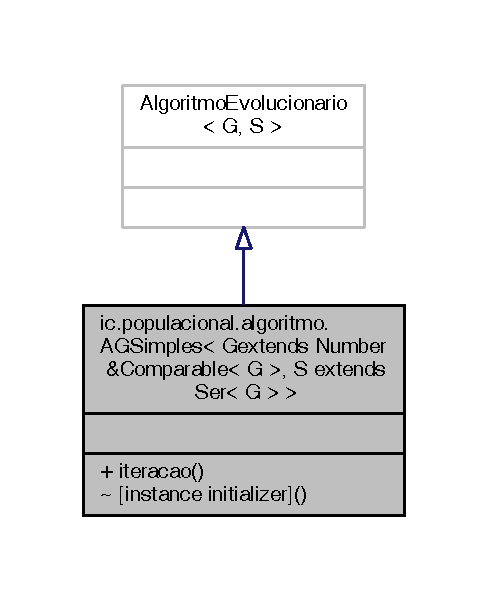
\includegraphics[width=234pt]{classic_1_1populacional_1_1algoritmo_1_1_a_g_simples_3_01_gextends_01_number_01_6_comparable_3_0908c421faf32439f86928e74347a3f5e}
\end{center}
\end{figure}


Diagrama de colaboração para ic.\-populacional.\-algoritmo.\-A\-G\-Simples$<$ Gextends Number \&Comparable$<$ G $>$, S extends Ser$<$ G $>$ $>$\-:\nopagebreak
\begin{figure}[H]
\begin{center}
\leavevmode
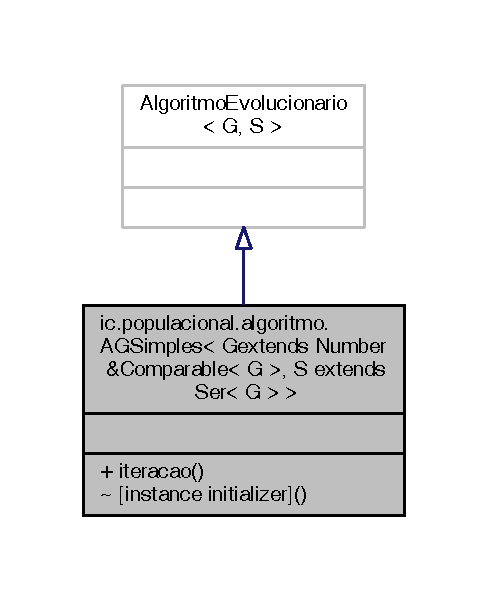
\includegraphics[width=234pt]{classic_1_1populacional_1_1algoritmo_1_1_a_g_simples_3_01_gextends_01_number_01_6_comparable_3_05ec3f2f1b04b7b3ba232b6087e927d58}
\end{center}
\end{figure}
\subsection*{Métodos Públicos}
\begin{DoxyCompactItemize}
\item 
void \hyperlink{classic_1_1populacional_1_1algoritmo_1_1_a_g_simples_3_01_gextends_01_number_01_6_comparable_3_0be0ec9d5f7dd5a82100acb38215a761d_af517e2be0edc10b8db274cd8a7cb59be}{iteracao} ()
\end{DoxyCompactItemize}


\subsection{Descrição Detalhada}
A\-G simples (S\-G\-A) ou canônico. 

Características\-: 
\begin{DoxyItemize}
\item Forma de Representação\-: Codificação binária/real; 
\item Operador de Recombinação\-: crossover de 1-\/ponto; 
\item Operador de Mutação\-: Bit-\/\-Flip com baixa probabilidade; 
\item Seleção dos Pais\-: Proporcional ao Fitness Geracional. 
\item Seleção dos Sobrevivente\-S\-: Geracional. 
\end{DoxyItemize}

\begin{DoxyAuthor}{Autor}
Victor de Lima Soares 
\end{DoxyAuthor}
\begin{DoxyVersion}{Versão}
1.\-0 
\end{DoxyVersion}

\begin{DoxyParams}{Parâmetros}
{\em $<$\-G$>$} & Classe do retorno da função objetivo (Grau de adaptação)\-: Atomic\-Integer, Atomic\-Long, Big\-Decimal, Big\-Integer, Byte, Double, Float, Integer, Long, Short. \\
\hline
{\em $<$\-S$>$} & Classe dos Seres \\
\hline
\end{DoxyParams}


\subsection{Métodos}
\hypertarget{classic_1_1populacional_1_1algoritmo_1_1_a_g_simples_3_01_gextends_01_number_01_6_comparable_3_0be0ec9d5f7dd5a82100acb38215a761d_af517e2be0edc10b8db274cd8a7cb59be}{\index{ic\-::populacional\-::algoritmo\-::\-A\-G\-Simples$<$ Gextends Number \&\-Comparable$<$ G $>$, S extends Ser$<$ G $>$ $>$@{ic\-::populacional\-::algoritmo\-::\-A\-G\-Simples$<$ Gextends Number \&\-Comparable$<$ G $>$, S extends Ser$<$ G $>$ $>$}!iteracao@{iteracao}}
\index{iteracao@{iteracao}!ic::populacional::algoritmo::AGSimples< Gextends Number &Comparable< G >, S extends Ser< G > >@{ic\-::populacional\-::algoritmo\-::\-A\-G\-Simples$<$ Gextends Number \&\-Comparable$<$ G $>$, S extends Ser$<$ G $>$ $>$}}
\subsubsection[{iteracao}]{\setlength{\rightskip}{0pt plus 5cm}void ic.\-populacional.\-algoritmo.\-A\-G\-Simples$<$ Gextends Number \&Comparable$<$ G $>$, S extends Ser$<$ G $>$ $>$.iteracao (
\begin{DoxyParamCaption}
{}
\end{DoxyParamCaption}
)}}\label{classic_1_1populacional_1_1algoritmo_1_1_a_g_simples_3_01_gextends_01_number_01_6_comparable_3_0be0ec9d5f7dd5a82100acb38215a761d_af517e2be0edc10b8db274cd8a7cb59be}


A documentação para esta classe foi gerada a partir do seguinte arquivo\-:\begin{DoxyCompactItemize}
\item 
C\-:/\-Users/\-Victor/workplace/\-Net\-Beans\-Projects/\-Inteligencia Computacional/src/ic/populacional/algoritmo/\hyperlink{_a_g_simples_8java}{A\-G\-Simples.\-java}\end{DoxyCompactItemize}

\hypertarget{classic_1_1populacional_1_1utilidades_1_1_aleatorios}{\section{Referência da Classe ic.\-populacional.\-utilidades.\-Aleatorios}
\label{classic_1_1populacional_1_1utilidades_1_1_aleatorios}\index{ic.\-populacional.\-utilidades.\-Aleatorios@{ic.\-populacional.\-utilidades.\-Aleatorios}}
}


Diagrama de colaboração para ic.\-populacional.\-utilidades.\-Aleatorios\-:\nopagebreak
\begin{figure}[H]
\begin{center}
\leavevmode
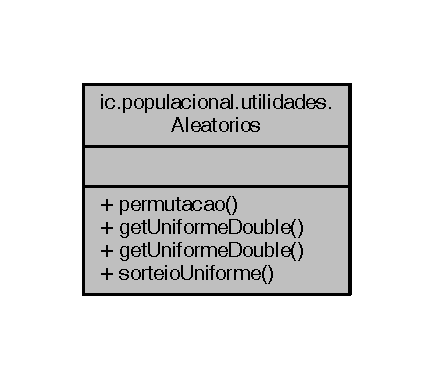
\includegraphics[width=208pt]{classic_1_1populacional_1_1utilidades_1_1_aleatorios__coll__graph}
\end{center}
\end{figure}
\subsection*{Métodos Públicos Estáticos}
\begin{DoxyCompactItemize}
\item 
static final List$<$ Integer $>$ \hyperlink{classic_1_1populacional_1_1utilidades_1_1_aleatorios_ac9a7a3a713982bd9d998a72af9505bca}{permutacao} (int inicio, int fim)
\begin{DoxyCompactList}\small\item\em Retorna n índices aleatórios em uma permutação de inteiros. \end{DoxyCompactList}\item 
static final double \hyperlink{classic_1_1populacional_1_1utilidades_1_1_aleatorios_ade30e7f2fcb5a65542f45463a7920406}{get\-Uniforme\-Double} ()
\begin{DoxyCompactList}\small\item\em Retorna um numero de ponto flutuante entre \mbox{[}0-\/1\mbox{]}. \end{DoxyCompactList}\item 
static final double \hyperlink{classic_1_1populacional_1_1utilidades_1_1_aleatorios_a1f014264b956136dea38ce9e3ae8e6ba}{get\-Uniforme\-Double} (Double a, Double b)
\begin{DoxyCompactList}\small\item\em Retorna um numero de ponto flutuante entre \mbox{[}a-\/b\mbox{]}. \end{DoxyCompactList}\item 
static boolean \hyperlink{classic_1_1populacional_1_1utilidades_1_1_aleatorios_a92ad4ea348ed7dd0fd3e400f2389abe4}{sorteio\-Uniforme} (double probabilidade\-De\-Sucesso)
\end{DoxyCompactItemize}


\subsection{Descrição Detalhada}
\begin{DoxyAuthor}{Autor}
Victor de Lima Soares 
\end{DoxyAuthor}


\subsection{Métodos}
\hypertarget{classic_1_1populacional_1_1utilidades_1_1_aleatorios_ade30e7f2fcb5a65542f45463a7920406}{\index{ic\-::populacional\-::utilidades\-::\-Aleatorios@{ic\-::populacional\-::utilidades\-::\-Aleatorios}!get\-Uniforme\-Double@{get\-Uniforme\-Double}}
\index{get\-Uniforme\-Double@{get\-Uniforme\-Double}!ic::populacional::utilidades::Aleatorios@{ic\-::populacional\-::utilidades\-::\-Aleatorios}}
\subsubsection[{get\-Uniforme\-Double}]{\setlength{\rightskip}{0pt plus 5cm}static final double ic.\-populacional.\-utilidades.\-Aleatorios.\-get\-Uniforme\-Double (
\begin{DoxyParamCaption}
{}
\end{DoxyParamCaption}
)\hspace{0.3cm}{\ttfamily [static]}}}\label{classic_1_1populacional_1_1utilidades_1_1_aleatorios_ade30e7f2fcb5a65542f45463a7920406}


Retorna um numero de ponto flutuante entre \mbox{[}0-\/1\mbox{]}. 

Distribuição uniforme.

\begin{DoxyReturn}{Retorna}
Número escolhido aleatoriamente. 
\end{DoxyReturn}


Este é o diagrama das funções que utilizam esta função\-:
\nopagebreak
\begin{figure}[H]
\begin{center}
\leavevmode
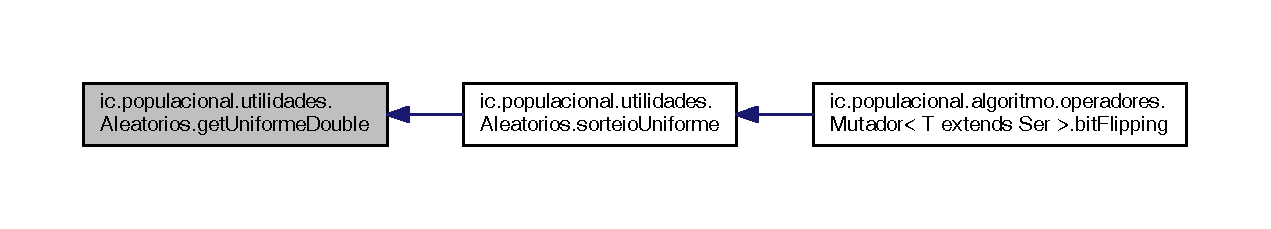
\includegraphics[width=350pt]{classic_1_1populacional_1_1utilidades_1_1_aleatorios_ade30e7f2fcb5a65542f45463a7920406_icgraph}
\end{center}
\end{figure}


\hypertarget{classic_1_1populacional_1_1utilidades_1_1_aleatorios_a1f014264b956136dea38ce9e3ae8e6ba}{\index{ic\-::populacional\-::utilidades\-::\-Aleatorios@{ic\-::populacional\-::utilidades\-::\-Aleatorios}!get\-Uniforme\-Double@{get\-Uniforme\-Double}}
\index{get\-Uniforme\-Double@{get\-Uniforme\-Double}!ic::populacional::utilidades::Aleatorios@{ic\-::populacional\-::utilidades\-::\-Aleatorios}}
\subsubsection[{get\-Uniforme\-Double}]{\setlength{\rightskip}{0pt plus 5cm}static final double ic.\-populacional.\-utilidades.\-Aleatorios.\-get\-Uniforme\-Double (
\begin{DoxyParamCaption}
\item[{Double}]{a, }
\item[{Double}]{b}
\end{DoxyParamCaption}
)\hspace{0.3cm}{\ttfamily [static]}}}\label{classic_1_1populacional_1_1utilidades_1_1_aleatorios_a1f014264b956136dea38ce9e3ae8e6ba}


Retorna um numero de ponto flutuante entre \mbox{[}a-\/b\mbox{]}. 

Distribuição uniforme.

\begin{DoxyReturn}{Retorna}
Número escolhido aleatoriamente. 
\end{DoxyReturn}
\hypertarget{classic_1_1populacional_1_1utilidades_1_1_aleatorios_ac9a7a3a713982bd9d998a72af9505bca}{\index{ic\-::populacional\-::utilidades\-::\-Aleatorios@{ic\-::populacional\-::utilidades\-::\-Aleatorios}!permutacao@{permutacao}}
\index{permutacao@{permutacao}!ic::populacional::utilidades::Aleatorios@{ic\-::populacional\-::utilidades\-::\-Aleatorios}}
\subsubsection[{permutacao}]{\setlength{\rightskip}{0pt plus 5cm}static final List$<$Integer$>$ ic.\-populacional.\-utilidades.\-Aleatorios.\-permutacao (
\begin{DoxyParamCaption}
\item[{int}]{inicio, }
\item[{int}]{fim}
\end{DoxyParamCaption}
)\hspace{0.3cm}{\ttfamily [static]}}}\label{classic_1_1populacional_1_1utilidades_1_1_aleatorios_ac9a7a3a713982bd9d998a72af9505bca}


Retorna n índices aleatórios em uma permutação de inteiros. 

Distribuição uniforme.


\begin{DoxyParams}{Parâmetros}
{\em inicio} & Menor número na permutação. \\
\hline
{\em fim} & Maior número na permutação. \\
\hline
\end{DoxyParams}
\begin{DoxyReturn}{Retorna}
Índices escolhidos aleatoriamente, sem uma permutação de inteiros. 
\end{DoxyReturn}


Este é o diagrama das funções que utilizam esta função\-:
\nopagebreak
\begin{figure}[H]
\begin{center}
\leavevmode
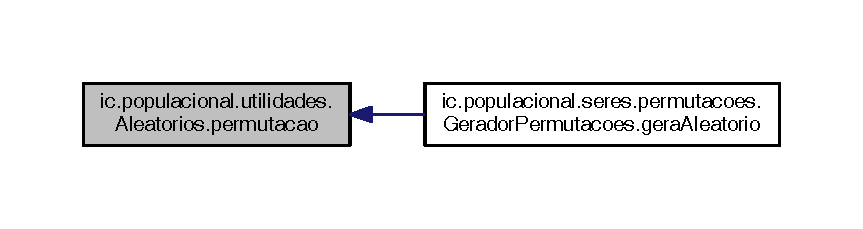
\includegraphics[width=350pt]{classic_1_1populacional_1_1utilidades_1_1_aleatorios_ac9a7a3a713982bd9d998a72af9505bca_icgraph}
\end{center}
\end{figure}


\hypertarget{classic_1_1populacional_1_1utilidades_1_1_aleatorios_a92ad4ea348ed7dd0fd3e400f2389abe4}{\index{ic\-::populacional\-::utilidades\-::\-Aleatorios@{ic\-::populacional\-::utilidades\-::\-Aleatorios}!sorteio\-Uniforme@{sorteio\-Uniforme}}
\index{sorteio\-Uniforme@{sorteio\-Uniforme}!ic::populacional::utilidades::Aleatorios@{ic\-::populacional\-::utilidades\-::\-Aleatorios}}
\subsubsection[{sorteio\-Uniforme}]{\setlength{\rightskip}{0pt plus 5cm}static boolean ic.\-populacional.\-utilidades.\-Aleatorios.\-sorteio\-Uniforme (
\begin{DoxyParamCaption}
\item[{double}]{probabilidade\-De\-Sucesso}
\end{DoxyParamCaption}
)\hspace{0.3cm}{\ttfamily [static]}}}\label{classic_1_1populacional_1_1utilidades_1_1_aleatorios_a92ad4ea348ed7dd0fd3e400f2389abe4}

\begin{DoxyParams}{Parâmetros}
{\em probabilidade\-De\-Sucesso} & \\
\hline
\end{DoxyParams}
\begin{DoxyReturn}{Retorna}

\end{DoxyReturn}


Este é o diagrama das funções utilizadas por esta função\-:\nopagebreak
\begin{figure}[H]
\begin{center}
\leavevmode
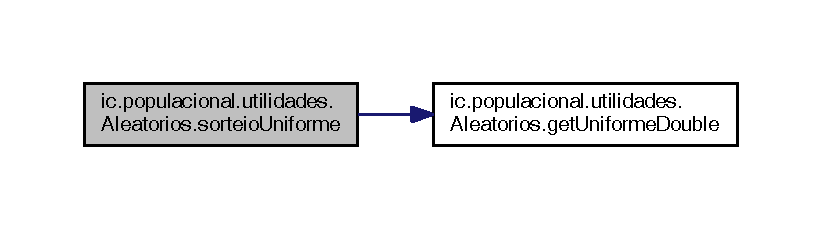
\includegraphics[width=350pt]{classic_1_1populacional_1_1utilidades_1_1_aleatorios_a92ad4ea348ed7dd0fd3e400f2389abe4_cgraph}
\end{center}
\end{figure}




Este é o diagrama das funções que utilizam esta função\-:
\nopagebreak
\begin{figure}[H]
\begin{center}
\leavevmode
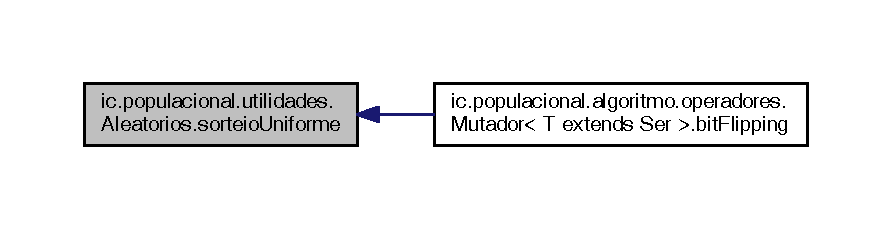
\includegraphics[width=350pt]{classic_1_1populacional_1_1utilidades_1_1_aleatorios_a92ad4ea348ed7dd0fd3e400f2389abe4_icgraph}
\end{center}
\end{figure}




A documentação para esta classe foi gerada a partir do seguinte arquivo\-:\begin{DoxyCompactItemize}
\item 
C\-:/\-Users/\-Victor/workplace/\-Net\-Beans\-Projects/\-Inteligencia Computacional/src/ic/populacional/utilidades/\hyperlink{_aleatorios_8java}{Aleatorios.\-java}\end{DoxyCompactItemize}

\hypertarget{classic_1_1populacional_1_1algoritmo_1_1_algoritmo_evolucionario_3_01_gextends_01_number_01_6_co1efdb05fe19a950b8d1e9e15f7d06254}{\section{Referência da Classe ic.\-populacional.\-algoritmo.\-Algoritmo\-Evolucionario$<$ Gextends Number \&Comparable$<$ G $>$, S extends Ser$<$ G $>$ $>$}
\label{classic_1_1populacional_1_1algoritmo_1_1_algoritmo_evolucionario_3_01_gextends_01_number_01_6_co1efdb05fe19a950b8d1e9e15f7d06254}\index{ic.\-populacional.\-algoritmo.\-Algoritmo\-Evolucionario$<$ Gextends Number \&\-Comparable$<$ G $>$, S extends Ser$<$ G $>$ $>$@{ic.\-populacional.\-algoritmo.\-Algoritmo\-Evolucionario$<$ Gextends Number \&\-Comparable$<$ G $>$, S extends Ser$<$ G $>$ $>$}}
}


Classe base para os Algoritmo Evolucionários.  




Diagrama de Hierarquia para ic.\-populacional.\-algoritmo.\-Algoritmo\-Evolucionario$<$ Gextends Number \&Comparable$<$ G $>$, S extends Ser$<$ G $>$ $>$\-:\nopagebreak
\begin{figure}[H]
\begin{center}
\leavevmode
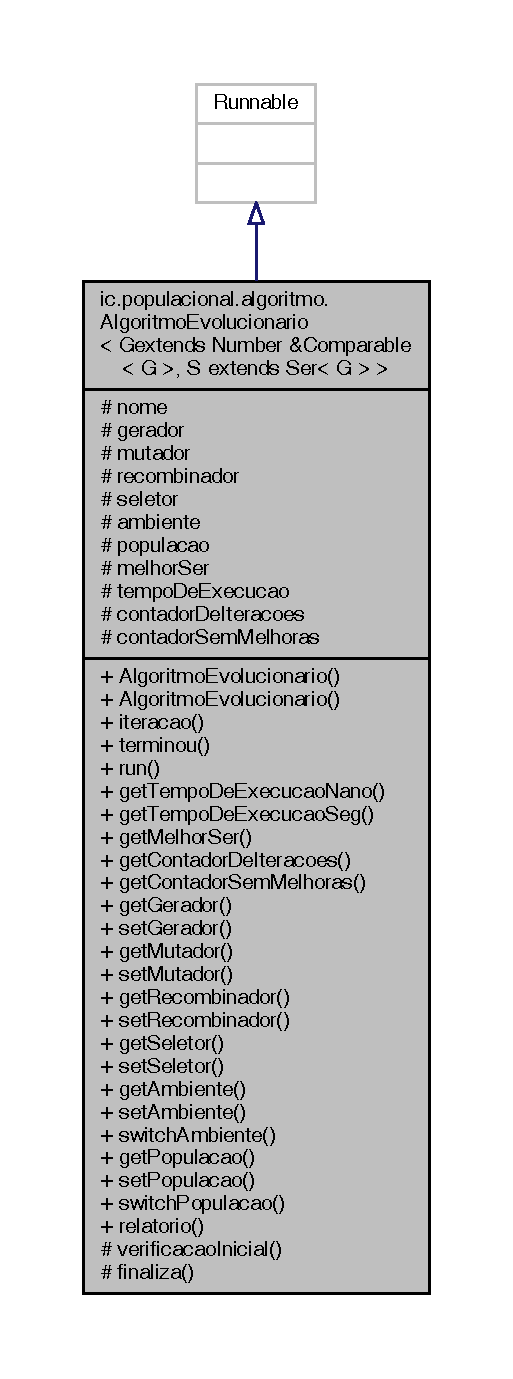
\includegraphics[height=550pt]{classic_1_1populacional_1_1algoritmo_1_1_algoritmo_evolucionario_3_01_gextends_01_number_01_6_co4c08ad55e259f326d7979b430087ff12}
\end{center}
\end{figure}


Diagrama de colaboração para ic.\-populacional.\-algoritmo.\-Algoritmo\-Evolucionario$<$ Gextends Number \&Comparable$<$ G $>$, S extends Ser$<$ G $>$ $>$\-:\nopagebreak
\begin{figure}[H]
\begin{center}
\leavevmode
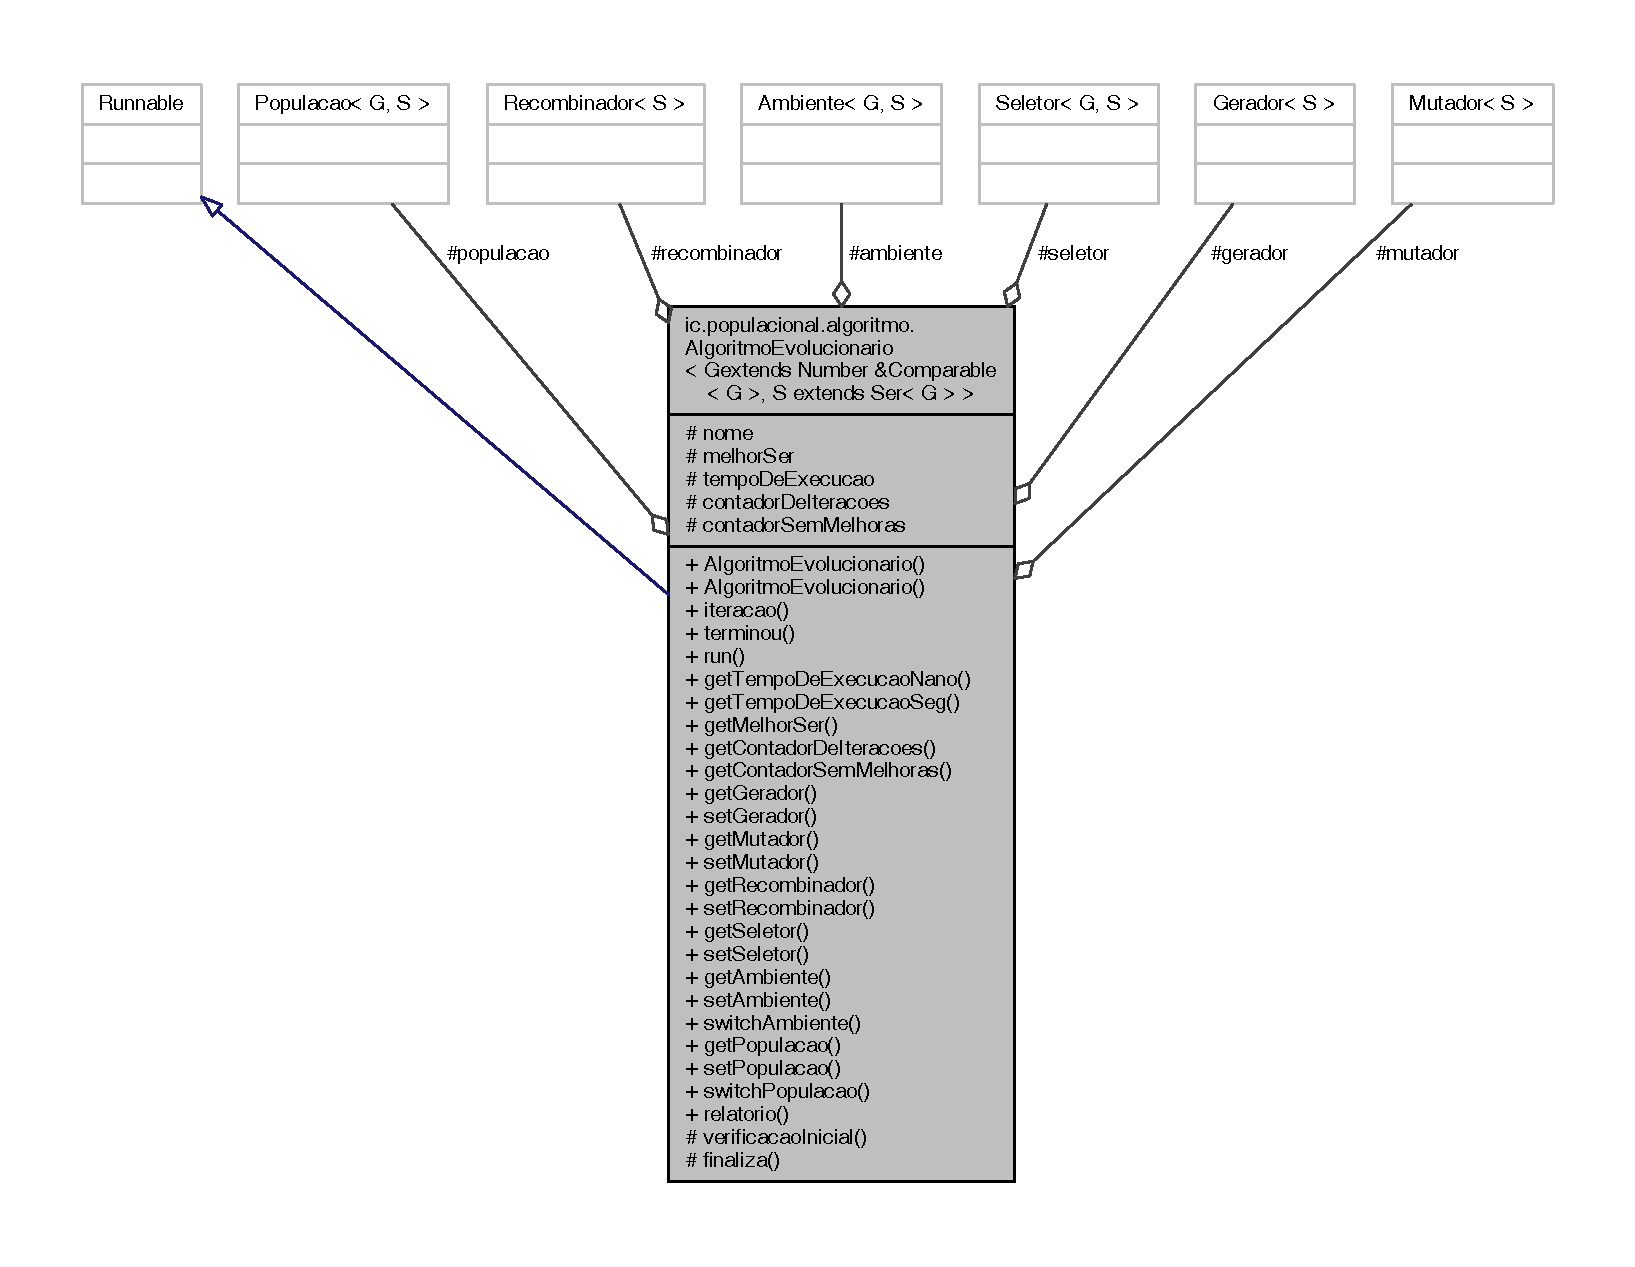
\includegraphics[width=350pt]{classic_1_1populacional_1_1algoritmo_1_1_algoritmo_evolucionario_3_01_gextends_01_number_01_6_coe0d94f23744d6c3f49b08c61bc2225e5}
\end{center}
\end{figure}
\subsection*{Métodos Públicos}
\begin{DoxyCompactItemize}
\item 
\hyperlink{classic_1_1populacional_1_1algoritmo_1_1_algoritmo_evolucionario_3_01_gextends_01_number_01_6_co1efdb05fe19a950b8d1e9e15f7d06254_a44bcf88506c92fbaf65cb3b223015004}{Algoritmo\-Evolucionario} ()
\begin{DoxyCompactList}\small\item\em Construtor padrão. \end{DoxyCompactList}\item 
\hyperlink{classic_1_1populacional_1_1algoritmo_1_1_algoritmo_evolucionario_3_01_gextends_01_number_01_6_co1efdb05fe19a950b8d1e9e15f7d06254_a5a2ad6905fc5f843bdc02d17ac9245e6}{Algoritmo\-Evolucionario} (Ambiente$<$ G, S $>$ \hyperlink{classic_1_1populacional_1_1algoritmo_1_1_algoritmo_evolucionario_3_01_gextends_01_number_01_6_co1efdb05fe19a950b8d1e9e15f7d06254_a7ccec051269f59db009703ae09400f54}{ambiente}, Populacao$<$ G, S $>$ \hyperlink{classic_1_1populacional_1_1algoritmo_1_1_algoritmo_evolucionario_3_01_gextends_01_number_01_6_co1efdb05fe19a950b8d1e9e15f7d06254_ac925832558d94f84dc90252371f8cb32}{populacao})
\begin{DoxyCompactList}\small\item\em Construtor. \end{DoxyCompactList}\item 
abstract void \hyperlink{classic_1_1populacional_1_1algoritmo_1_1_algoritmo_evolucionario_3_01_gextends_01_number_01_6_co1efdb05fe19a950b8d1e9e15f7d06254_a1f67fd61bb31bc952dd7a8afd03ad1af}{iteracao} ()
\begin{DoxyCompactList}\small\item\em Define uma iteração. \end{DoxyCompactList}\item 
abstract boolean \hyperlink{classic_1_1populacional_1_1algoritmo_1_1_algoritmo_evolucionario_3_01_gextends_01_number_01_6_co1efdb05fe19a950b8d1e9e15f7d06254_a81f74bfb66080cfc85593d997d4f973c}{terminou} ()
\begin{DoxyCompactList}\small\item\em Condição de parada. \end{DoxyCompactList}\item 
void \hyperlink{classic_1_1populacional_1_1algoritmo_1_1_algoritmo_evolucionario_3_01_gextends_01_number_01_6_co1efdb05fe19a950b8d1e9e15f7d06254_a0fd82664e0e022b2e965923560830f9a}{run} ()
\begin{DoxyCompactList}\small\item\em Executa o algoritmo. \end{DoxyCompactList}\item 
long \hyperlink{classic_1_1populacional_1_1algoritmo_1_1_algoritmo_evolucionario_3_01_gextends_01_number_01_6_co1efdb05fe19a950b8d1e9e15f7d06254_af9da640a882ddb1eb17ad360c109b530}{get\-Tempo\-De\-Execucao\-Nano} ()
\begin{DoxyCompactList}\small\item\em Retorna Tempo de execução (n\-Seg). \end{DoxyCompactList}\item 
Double \hyperlink{classic_1_1populacional_1_1algoritmo_1_1_algoritmo_evolucionario_3_01_gextends_01_number_01_6_co1efdb05fe19a950b8d1e9e15f7d06254_a9ccb62ffa2361974547cc763de474fc2}{get\-Tempo\-De\-Execucao\-Seg} ()
\begin{DoxyCompactList}\small\item\em Retorna Tempo de execução (Seg). \end{DoxyCompactList}\item 
S \hyperlink{classic_1_1populacional_1_1algoritmo_1_1_algoritmo_evolucionario_3_01_gextends_01_number_01_6_co1efdb05fe19a950b8d1e9e15f7d06254_ae50ff320a0f435c5e2d2eaaf58129680}{get\-Melhor\-Ser} ()
\begin{DoxyCompactList}\small\item\em Retorna o melhor ser encontrado em todas as iterações. \end{DoxyCompactList}\item 
int \hyperlink{classic_1_1populacional_1_1algoritmo_1_1_algoritmo_evolucionario_3_01_gextends_01_number_01_6_co1efdb05fe19a950b8d1e9e15f7d06254_adec275a30d0db288c2408b58370a8ae3}{get\-Contador\-De\-Iteracoes} ()
\begin{DoxyCompactList}\small\item\em Retorna o valor do contador de iterações. \end{DoxyCompactList}\item 
int \hyperlink{classic_1_1populacional_1_1algoritmo_1_1_algoritmo_evolucionario_3_01_gextends_01_number_01_6_co1efdb05fe19a950b8d1e9e15f7d06254_a60040842d3e086afaac59479914f2d4c}{get\-Contador\-Sem\-Melhoras} ()
\begin{DoxyCompactList}\small\item\em Retorna o valor do contador de iterações sem melhoras. \end{DoxyCompactList}\item 
Gerador$<$ S $>$ \hyperlink{classic_1_1populacional_1_1algoritmo_1_1_algoritmo_evolucionario_3_01_gextends_01_number_01_6_co1efdb05fe19a950b8d1e9e15f7d06254_afe7d44c986de2ed75fc4d0dc1e279715}{get\-Gerador} ()
\begin{DoxyCompactList}\small\item\em Retorna o operador de geração utilizado. \end{DoxyCompactList}\item 
void \hyperlink{classic_1_1populacional_1_1algoritmo_1_1_algoritmo_evolucionario_3_01_gextends_01_number_01_6_co1efdb05fe19a950b8d1e9e15f7d06254_ad98dea12ac5aa49c3aedd64731277590}{set\-Gerador} (Gerador$<$ S $>$ \hyperlink{classic_1_1populacional_1_1algoritmo_1_1_algoritmo_evolucionario_3_01_gextends_01_number_01_6_co1efdb05fe19a950b8d1e9e15f7d06254_a2154470c0a2b1ae8fd1728d82217b40d}{gerador})
\begin{DoxyCompactList}\small\item\em Atribui um novo operador de geração ao algoritmo. \end{DoxyCompactList}\item 
Mutador$<$ S $>$ \hyperlink{classic_1_1populacional_1_1algoritmo_1_1_algoritmo_evolucionario_3_01_gextends_01_number_01_6_co1efdb05fe19a950b8d1e9e15f7d06254_a49c46ab9b5bfaab7199ab4ab996fc66c}{get\-Mutador} ()
\begin{DoxyCompactList}\small\item\em Retorna o operador de mutação utilizado. \end{DoxyCompactList}\item 
void \hyperlink{classic_1_1populacional_1_1algoritmo_1_1_algoritmo_evolucionario_3_01_gextends_01_number_01_6_co1efdb05fe19a950b8d1e9e15f7d06254_aa29043d9ec8f15f5c12146ef87f74e75}{set\-Mutador} (Mutador$<$ S $>$ \hyperlink{classic_1_1populacional_1_1algoritmo_1_1_algoritmo_evolucionario_3_01_gextends_01_number_01_6_co1efdb05fe19a950b8d1e9e15f7d06254_a87cb55bc36af5a64c095d7030449eab2}{mutador})
\begin{DoxyCompactList}\small\item\em Atribui um novo operador de mutação ao algoritmo. \end{DoxyCompactList}\item 
Recombinador$<$ S $>$ \hyperlink{classic_1_1populacional_1_1algoritmo_1_1_algoritmo_evolucionario_3_01_gextends_01_number_01_6_co1efdb05fe19a950b8d1e9e15f7d06254_a1dc1bba750535e8c0332be177fad63fa}{get\-Recombinador} ()
\begin{DoxyCompactList}\small\item\em Retorna o operador de recombinação utilizado. \end{DoxyCompactList}\item 
void \hyperlink{classic_1_1populacional_1_1algoritmo_1_1_algoritmo_evolucionario_3_01_gextends_01_number_01_6_co1efdb05fe19a950b8d1e9e15f7d06254_ae2ec6e66337c0c1075767f9222ecaa20}{set\-Recombinador} (Recombinador$<$ S $>$ \hyperlink{classic_1_1populacional_1_1algoritmo_1_1_algoritmo_evolucionario_3_01_gextends_01_number_01_6_co1efdb05fe19a950b8d1e9e15f7d06254_a5ca76dcf5ea537ba8af6e1b66559de43}{recombinador})
\begin{DoxyCompactList}\small\item\em Atribui um novo operador de recombinação ao algoritmo. \end{DoxyCompactList}\item 
Seletor$<$ G, S $>$ \hyperlink{classic_1_1populacional_1_1algoritmo_1_1_algoritmo_evolucionario_3_01_gextends_01_number_01_6_co1efdb05fe19a950b8d1e9e15f7d06254_abf133c60cd2d87d98243c232df8a57f9}{get\-Seletor} ()
\begin{DoxyCompactList}\small\item\em Retorna o operador de seleção utilizado. \end{DoxyCompactList}\item 
void \hyperlink{classic_1_1populacional_1_1algoritmo_1_1_algoritmo_evolucionario_3_01_gextends_01_number_01_6_co1efdb05fe19a950b8d1e9e15f7d06254_a359a39d12caae7697213b535e4c60b74}{set\-Seletor} (Seletor$<$ G, S $>$ \hyperlink{classic_1_1populacional_1_1algoritmo_1_1_algoritmo_evolucionario_3_01_gextends_01_number_01_6_co1efdb05fe19a950b8d1e9e15f7d06254_ab55978264aecc3e7faa54575dcb3c95b}{seletor})
\begin{DoxyCompactList}\small\item\em Atribui um novo operador de seleção ao algoritmo. \end{DoxyCompactList}\item 
Ambiente$<$ G, S $>$ \hyperlink{classic_1_1populacional_1_1algoritmo_1_1_algoritmo_evolucionario_3_01_gextends_01_number_01_6_co1efdb05fe19a950b8d1e9e15f7d06254_a998385f45e2ac36c869623a549e26898}{get\-Ambiente} ()
\begin{DoxyCompactList}\small\item\em Retorna o ambiente do algoritmo. \end{DoxyCompactList}\item 
void \hyperlink{classic_1_1populacional_1_1algoritmo_1_1_algoritmo_evolucionario_3_01_gextends_01_number_01_6_co1efdb05fe19a950b8d1e9e15f7d06254_a68db18fec4322f9ec81e1b958162b655}{set\-Ambiente} (Ambiente$<$ G, S $>$ \hyperlink{classic_1_1populacional_1_1algoritmo_1_1_algoritmo_evolucionario_3_01_gextends_01_number_01_6_co1efdb05fe19a950b8d1e9e15f7d06254_a7ccec051269f59db009703ae09400f54}{ambiente})
\begin{DoxyCompactList}\small\item\em Atribui um novo ambiente ao algoritmo, sem avaliação dos seres. \end{DoxyCompactList}\item 
void \hyperlink{classic_1_1populacional_1_1algoritmo_1_1_algoritmo_evolucionario_3_01_gextends_01_number_01_6_co1efdb05fe19a950b8d1e9e15f7d06254_a85180b600cd1b09c637cd7be58509a7e}{switch\-Ambiente} (Ambiente$<$ G, S $>$ \hyperlink{classic_1_1populacional_1_1algoritmo_1_1_algoritmo_evolucionario_3_01_gextends_01_number_01_6_co1efdb05fe19a950b8d1e9e15f7d06254_a7ccec051269f59db009703ae09400f54}{ambiente})
\begin{DoxyCompactList}\small\item\em Atribui um novo ambiente ao algoritmo, com reavaliação. \end{DoxyCompactList}\item 
Populacao$<$ G, S $>$ \hyperlink{classic_1_1populacional_1_1algoritmo_1_1_algoritmo_evolucionario_3_01_gextends_01_number_01_6_co1efdb05fe19a950b8d1e9e15f7d06254_a88c00c7d51d16c559ccb8392f6892d90}{get\-Populacao} ()
\begin{DoxyCompactList}\small\item\em Retorna a população do algoritmo. \end{DoxyCompactList}\item 
void \hyperlink{classic_1_1populacional_1_1algoritmo_1_1_algoritmo_evolucionario_3_01_gextends_01_number_01_6_co1efdb05fe19a950b8d1e9e15f7d06254_aaf17db98cce445b6f757b9c37810327a}{set\-Populacao} (Populacao$<$ G, S $>$ \hyperlink{classic_1_1populacional_1_1algoritmo_1_1_algoritmo_evolucionario_3_01_gextends_01_number_01_6_co1efdb05fe19a950b8d1e9e15f7d06254_ac925832558d94f84dc90252371f8cb32}{populacao})
\begin{DoxyCompactList}\small\item\em Atribui uma nova população ao algoritmo, sem avaliação dos seres. \end{DoxyCompactList}\item 
void \hyperlink{classic_1_1populacional_1_1algoritmo_1_1_algoritmo_evolucionario_3_01_gextends_01_number_01_6_co1efdb05fe19a950b8d1e9e15f7d06254_a8fc2d9d6a132efd494cf3a8cd44d5446}{switch\-Populacao} (Populacao$<$ G, S $>$ \hyperlink{classic_1_1populacional_1_1algoritmo_1_1_algoritmo_evolucionario_3_01_gextends_01_number_01_6_co1efdb05fe19a950b8d1e9e15f7d06254_ac925832558d94f84dc90252371f8cb32}{populacao})
\begin{DoxyCompactList}\small\item\em Atribui uma nova população ao algoritmo, com avaliação. \end{DoxyCompactList}\item 
String \hyperlink{classic_1_1populacional_1_1algoritmo_1_1_algoritmo_evolucionario_3_01_gextends_01_number_01_6_co1efdb05fe19a950b8d1e9e15f7d06254_a962b55611f2dc3366b6a67328053eaa6}{relatorio} ()
\begin{DoxyCompactList}\small\item\em Realiza a compilação dos dados coletados durante a execução do algoritmo. \end{DoxyCompactList}\end{DoxyCompactItemize}
\subsection*{Métodos Protegidos}
\begin{DoxyCompactItemize}
\item 
void \hyperlink{classic_1_1populacional_1_1algoritmo_1_1_algoritmo_evolucionario_3_01_gextends_01_number_01_6_co1efdb05fe19a950b8d1e9e15f7d06254_a5011151c232024dcf10891066b3b47b9}{verificacao\-Inicial} ()  throws Illegal\-State\-Exception 
\begin{DoxyCompactList}\small\item\em Verifica as condições necessárias para execução do algoritmo. \end{DoxyCompactList}\item 
void \hyperlink{classic_1_1populacional_1_1algoritmo_1_1_algoritmo_evolucionario_3_01_gextends_01_number_01_6_co1efdb05fe19a950b8d1e9e15f7d06254_a73a87fc597bdd4c7c583514062171f7d}{finaliza} ()
\begin{DoxyCompactList}\small\item\em Função a ser executada após o termino das iterações. \end{DoxyCompactList}\end{DoxyCompactItemize}
\subsection*{Atributos Protegidos}
\begin{DoxyCompactItemize}
\item 
String \hyperlink{classic_1_1populacional_1_1algoritmo_1_1_algoritmo_evolucionario_3_01_gextends_01_number_01_6_co1efdb05fe19a950b8d1e9e15f7d06254_a551c112a0f4ce635cc81478ce2fd13e0}{nome}
\item 
Gerador$<$ S $>$ \hyperlink{classic_1_1populacional_1_1algoritmo_1_1_algoritmo_evolucionario_3_01_gextends_01_number_01_6_co1efdb05fe19a950b8d1e9e15f7d06254_a2154470c0a2b1ae8fd1728d82217b40d}{gerador}
\item 
Mutador$<$ S $>$ \hyperlink{classic_1_1populacional_1_1algoritmo_1_1_algoritmo_evolucionario_3_01_gextends_01_number_01_6_co1efdb05fe19a950b8d1e9e15f7d06254_a87cb55bc36af5a64c095d7030449eab2}{mutador}
\item 
Recombinador$<$ S $>$ \hyperlink{classic_1_1populacional_1_1algoritmo_1_1_algoritmo_evolucionario_3_01_gextends_01_number_01_6_co1efdb05fe19a950b8d1e9e15f7d06254_a5ca76dcf5ea537ba8af6e1b66559de43}{recombinador}
\item 
Seletor$<$ G, S $>$ \hyperlink{classic_1_1populacional_1_1algoritmo_1_1_algoritmo_evolucionario_3_01_gextends_01_number_01_6_co1efdb05fe19a950b8d1e9e15f7d06254_ab55978264aecc3e7faa54575dcb3c95b}{seletor}
\item 
Ambiente$<$ G, S $>$ \hyperlink{classic_1_1populacional_1_1algoritmo_1_1_algoritmo_evolucionario_3_01_gextends_01_number_01_6_co1efdb05fe19a950b8d1e9e15f7d06254_a7ccec051269f59db009703ae09400f54}{ambiente}
\item 
Populacao$<$ G, S $>$ \hyperlink{classic_1_1populacional_1_1algoritmo_1_1_algoritmo_evolucionario_3_01_gextends_01_number_01_6_co1efdb05fe19a950b8d1e9e15f7d06254_ac925832558d94f84dc90252371f8cb32}{populacao}
\item 
S \hyperlink{classic_1_1populacional_1_1algoritmo_1_1_algoritmo_evolucionario_3_01_gextends_01_number_01_6_co1efdb05fe19a950b8d1e9e15f7d06254_a8a0306073891705183ac1cf667280589}{melhor\-Ser}
\item 
long \hyperlink{classic_1_1populacional_1_1algoritmo_1_1_algoritmo_evolucionario_3_01_gextends_01_number_01_6_co1efdb05fe19a950b8d1e9e15f7d06254_a8068592ee1b2603c5dbf52b399fb5bcf}{tempo\-De\-Execucao}
\item 
int \hyperlink{classic_1_1populacional_1_1algoritmo_1_1_algoritmo_evolucionario_3_01_gextends_01_number_01_6_co1efdb05fe19a950b8d1e9e15f7d06254_a68e92a3567c0973b579a70a9608d41d2}{contador\-De\-Iteracoes} = 0
\item 
int \hyperlink{classic_1_1populacional_1_1algoritmo_1_1_algoritmo_evolucionario_3_01_gextends_01_number_01_6_co1efdb05fe19a950b8d1e9e15f7d06254_adc778b6504cca0e8e4c346498dab8cc9}{contador\-Sem\-Melhoras} = 0
\end{DoxyCompactItemize}


\subsection{Descrição Detalhada}
Classe base para os Algoritmo Evolucionários. 

\begin{DoxyAuthor}{Autor}
Victor de Lima Soares 
\end{DoxyAuthor}
\begin{DoxyVersion}{Versão}
1.\-0
\end{DoxyVersion}

\begin{DoxyParams}{Parâmetros}
{\em $<$\-G$>$} & Classe do retorno da função objetivo (Grau de adaptação)\-: Atomic\-Integer, Atomic\-Long, Big\-Decimal, Big\-Integer, Byte, Double, Float, Integer, Long, Short. \\
\hline
{\em $<$\-S$>$} & Classe dos Seres. \\
\hline
\end{DoxyParams}


\subsection{Construtores \& Destrutores}
\hypertarget{classic_1_1populacional_1_1algoritmo_1_1_algoritmo_evolucionario_3_01_gextends_01_number_01_6_co1efdb05fe19a950b8d1e9e15f7d06254_a44bcf88506c92fbaf65cb3b223015004}{\index{ic\-::populacional\-::algoritmo\-::\-Algoritmo\-Evolucionario$<$ Gextends Number \&\-Comparable$<$ G $>$, S extends Ser$<$ G $>$ $>$@{ic\-::populacional\-::algoritmo\-::\-Algoritmo\-Evolucionario$<$ Gextends Number \&\-Comparable$<$ G $>$, S extends Ser$<$ G $>$ $>$}!Algoritmo\-Evolucionario@{Algoritmo\-Evolucionario}}
\index{Algoritmo\-Evolucionario@{Algoritmo\-Evolucionario}!ic::populacional::algoritmo::AlgoritmoEvolucionario< Gextends Number &Comparable< G >, S extends Ser< G > >@{ic\-::populacional\-::algoritmo\-::\-Algoritmo\-Evolucionario$<$ Gextends Number \&\-Comparable$<$ G $>$, S extends Ser$<$ G $>$ $>$}}
\subsubsection[{Algoritmo\-Evolucionario}]{\setlength{\rightskip}{0pt plus 5cm}ic.\-populacional.\-algoritmo.\-Algoritmo\-Evolucionario$<$ Gextends Number \&Comparable$<$ G $>$, S extends Ser$<$ G $>$ $>$.Algoritmo\-Evolucionario (
\begin{DoxyParamCaption}
{}
\end{DoxyParamCaption}
)}}\label{classic_1_1populacional_1_1algoritmo_1_1_algoritmo_evolucionario_3_01_gextends_01_number_01_6_co1efdb05fe19a950b8d1e9e15f7d06254_a44bcf88506c92fbaf65cb3b223015004}


Construtor padrão. 

Construtor padrão, para montagem do algoritmo por estágios – através do uso das funções {\itshape set}.

Cada componente do algoritmo deve ser atribuído antes da execução do mesmo, sendo obrigatórios uma população inicial e um ambiente. Os demais componentes (operadores), devem ser incluídos se exigidos pela função \hyperlink{classic_1_1populacional_1_1algoritmo_1_1_algoritmo_evolucionario_3_01_gextends_01_number_01_6_co1efdb05fe19a950b8d1e9e15f7d06254_a1f67fd61bb31bc952dd7a8afd03ad1af}{iteracao()}. 

\begin{DoxySince}{Desde}
1.\-0
\end{DoxySince}
\begin{DoxySeeAlso}{Veja também}
\hyperlink{classic_1_1populacional_1_1algoritmo_1_1_algoritmo_evolucionario_3_01_gextends_01_number_01_6_co1efdb05fe19a950b8d1e9e15f7d06254_aaf17db98cce445b6f757b9c37810327a}{set\-Populacao}(inteligencia\-Computacional.\-evolucioria.\-Populacao) 

\hyperlink{classic_1_1populacional_1_1algoritmo_1_1_algoritmo_evolucionario_3_01_gextends_01_number_01_6_co1efdb05fe19a950b8d1e9e15f7d06254_a68db18fec4322f9ec81e1b958162b655}{set\-Ambiente}(inteligencia\-Computacional.\-evolucioria.\-Ambiente) 

\hyperlink{classic_1_1populacional_1_1algoritmo_1_1_algoritmo_evolucionario_3_01_gextends_01_number_01_6_co1efdb05fe19a950b8d1e9e15f7d06254_ad98dea12ac5aa49c3aedd64731277590}{set\-Gerador}(inteligencia\-Computacional.\-evolucioria.\-algoritmo.\-operadores.\-Gerador) 

\hyperlink{classic_1_1populacional_1_1algoritmo_1_1_algoritmo_evolucionario_3_01_gextends_01_number_01_6_co1efdb05fe19a950b8d1e9e15f7d06254_ae2ec6e66337c0c1075767f9222ecaa20}{set\-Recombinador}(inteligencia\-Computacional.\-evolucioria.\-algoritmo.\-operadores.\-Recombinador) 

\hyperlink{classic_1_1populacional_1_1algoritmo_1_1_algoritmo_evolucionario_3_01_gextends_01_number_01_6_co1efdb05fe19a950b8d1e9e15f7d06254_aa29043d9ec8f15f5c12146ef87f74e75}{set\-Mutador}(inteligencia\-Computacional.\-evolucioria.\-algoritmo.\-operadores.\-Mutador) 

\hyperlink{classic_1_1populacional_1_1algoritmo_1_1_algoritmo_evolucionario_3_01_gextends_01_number_01_6_co1efdb05fe19a950b8d1e9e15f7d06254_a359a39d12caae7697213b535e4c60b74}{set\-Seletor}(inteligencia\-Computacional.\-evolucioria.\-algoritmo.\-operadores.\-Seletor) 
\end{DoxySeeAlso}
\hypertarget{classic_1_1populacional_1_1algoritmo_1_1_algoritmo_evolucionario_3_01_gextends_01_number_01_6_co1efdb05fe19a950b8d1e9e15f7d06254_a5a2ad6905fc5f843bdc02d17ac9245e6}{\index{ic\-::populacional\-::algoritmo\-::\-Algoritmo\-Evolucionario$<$ Gextends Number \&\-Comparable$<$ G $>$, S extends Ser$<$ G $>$ $>$@{ic\-::populacional\-::algoritmo\-::\-Algoritmo\-Evolucionario$<$ Gextends Number \&\-Comparable$<$ G $>$, S extends Ser$<$ G $>$ $>$}!Algoritmo\-Evolucionario@{Algoritmo\-Evolucionario}}
\index{Algoritmo\-Evolucionario@{Algoritmo\-Evolucionario}!ic::populacional::algoritmo::AlgoritmoEvolucionario< Gextends Number &Comparable< G >, S extends Ser< G > >@{ic\-::populacional\-::algoritmo\-::\-Algoritmo\-Evolucionario$<$ Gextends Number \&\-Comparable$<$ G $>$, S extends Ser$<$ G $>$ $>$}}
\subsubsection[{Algoritmo\-Evolucionario}]{\setlength{\rightskip}{0pt plus 5cm}ic.\-populacional.\-algoritmo.\-Algoritmo\-Evolucionario$<$ Gextends Number \&Comparable$<$ G $>$, S extends Ser$<$ G $>$ $>$.Algoritmo\-Evolucionario (
\begin{DoxyParamCaption}
\item[{Ambiente$<$ G, S $>$}]{ambiente, }
\item[{Populacao$<$ G, S $>$}]{populacao}
\end{DoxyParamCaption}
)}}\label{classic_1_1populacional_1_1algoritmo_1_1_algoritmo_evolucionario_3_01_gextends_01_number_01_6_co1efdb05fe19a950b8d1e9e15f7d06254_a5a2ad6905fc5f843bdc02d17ac9245e6}


Construtor. 

Construtor para fazer a atribuição inicial do ambiente e da população. 

Cada componente do algoritmo deve ser atribuído antes da execução do mesmo, sendo obrigatórios uma população inicial e um ambiente. Os demais componentes (operadores), devem ser incluídos se exigidos pela função \hyperlink{classic_1_1populacional_1_1algoritmo_1_1_algoritmo_evolucionario_3_01_gextends_01_number_01_6_co1efdb05fe19a950b8d1e9e15f7d06254_a1f67fd61bb31bc952dd7a8afd03ad1af}{iteracao()}. 

\begin{DoxySince}{Desde}
1.\-0 
\end{DoxySince}

\begin{DoxyParams}{Parâmetros}
{\em ambiente} & Ambiente para o algoritmo. \\
\hline
{\em populacao} & População inicial.\\
\hline
\end{DoxyParams}
\begin{DoxySeeAlso}{Veja também}
\hyperlink{classic_1_1populacional_1_1algoritmo_1_1_algoritmo_evolucionario_3_01_gextends_01_number_01_6_co1efdb05fe19a950b8d1e9e15f7d06254_aaf17db98cce445b6f757b9c37810327a}{set\-Populacao}(inteligencia\-Computacional.\-evolucioria.\-Populacao) 

\hyperlink{classic_1_1populacional_1_1algoritmo_1_1_algoritmo_evolucionario_3_01_gextends_01_number_01_6_co1efdb05fe19a950b8d1e9e15f7d06254_a68db18fec4322f9ec81e1b958162b655}{set\-Ambiente}(inteligencia\-Computacional.\-evolucioria.\-Ambiente) 

\hyperlink{classic_1_1populacional_1_1algoritmo_1_1_algoritmo_evolucionario_3_01_gextends_01_number_01_6_co1efdb05fe19a950b8d1e9e15f7d06254_ad98dea12ac5aa49c3aedd64731277590}{set\-Gerador}(inteligencia\-Computacional.\-evolucioria.\-algoritmo.\-operadores.\-Gerador) 

\hyperlink{classic_1_1populacional_1_1algoritmo_1_1_algoritmo_evolucionario_3_01_gextends_01_number_01_6_co1efdb05fe19a950b8d1e9e15f7d06254_ae2ec6e66337c0c1075767f9222ecaa20}{set\-Recombinador}(inteligencia\-Computacional.\-evolucioria.\-algoritmo.\-operadores.\-Recombinador) 

\hyperlink{classic_1_1populacional_1_1algoritmo_1_1_algoritmo_evolucionario_3_01_gextends_01_number_01_6_co1efdb05fe19a950b8d1e9e15f7d06254_aa29043d9ec8f15f5c12146ef87f74e75}{set\-Mutador}(inteligencia\-Computacional.\-evolucioria.\-algoritmo.\-operadores.\-Mutador) 

\hyperlink{classic_1_1populacional_1_1algoritmo_1_1_algoritmo_evolucionario_3_01_gextends_01_number_01_6_co1efdb05fe19a950b8d1e9e15f7d06254_a359a39d12caae7697213b535e4c60b74}{set\-Seletor}(inteligencia\-Computacional.\-evolucioria.\-algoritmo.\-operadores.\-Seletor) 
\end{DoxySeeAlso}


\subsection{Métodos}
\hypertarget{classic_1_1populacional_1_1algoritmo_1_1_algoritmo_evolucionario_3_01_gextends_01_number_01_6_co1efdb05fe19a950b8d1e9e15f7d06254_a73a87fc597bdd4c7c583514062171f7d}{\index{ic\-::populacional\-::algoritmo\-::\-Algoritmo\-Evolucionario$<$ Gextends Number \&\-Comparable$<$ G $>$, S extends Ser$<$ G $>$ $>$@{ic\-::populacional\-::algoritmo\-::\-Algoritmo\-Evolucionario$<$ Gextends Number \&\-Comparable$<$ G $>$, S extends Ser$<$ G $>$ $>$}!finaliza@{finaliza}}
\index{finaliza@{finaliza}!ic::populacional::algoritmo::AlgoritmoEvolucionario< Gextends Number &Comparable< G >, S extends Ser< G > >@{ic\-::populacional\-::algoritmo\-::\-Algoritmo\-Evolucionario$<$ Gextends Number \&\-Comparable$<$ G $>$, S extends Ser$<$ G $>$ $>$}}
\subsubsection[{finaliza}]{\setlength{\rightskip}{0pt plus 5cm}void ic.\-populacional.\-algoritmo.\-Algoritmo\-Evolucionario$<$ Gextends Number \&Comparable$<$ G $>$, S extends Ser$<$ G $>$ $>$.finaliza (
\begin{DoxyParamCaption}
{}
\end{DoxyParamCaption}
)\hspace{0.3cm}{\ttfamily [protected]}}}\label{classic_1_1populacional_1_1algoritmo_1_1_algoritmo_evolucionario_3_01_gextends_01_number_01_6_co1efdb05fe19a950b8d1e9e15f7d06254_a73a87fc597bdd4c7c583514062171f7d}


Função a ser executada após o termino das iterações. 

A realização de uma busca local pode ser um exemplo de aplicação. 

Essa função é considerada no calculo do tempo de execução. 

\begin{DoxySince}{Desde}
1.\-0 
\end{DoxySince}
\hypertarget{classic_1_1populacional_1_1algoritmo_1_1_algoritmo_evolucionario_3_01_gextends_01_number_01_6_co1efdb05fe19a950b8d1e9e15f7d06254_a998385f45e2ac36c869623a549e26898}{\index{ic\-::populacional\-::algoritmo\-::\-Algoritmo\-Evolucionario$<$ Gextends Number \&\-Comparable$<$ G $>$, S extends Ser$<$ G $>$ $>$@{ic\-::populacional\-::algoritmo\-::\-Algoritmo\-Evolucionario$<$ Gextends Number \&\-Comparable$<$ G $>$, S extends Ser$<$ G $>$ $>$}!get\-Ambiente@{get\-Ambiente}}
\index{get\-Ambiente@{get\-Ambiente}!ic::populacional::algoritmo::AlgoritmoEvolucionario< Gextends Number &Comparable< G >, S extends Ser< G > >@{ic\-::populacional\-::algoritmo\-::\-Algoritmo\-Evolucionario$<$ Gextends Number \&\-Comparable$<$ G $>$, S extends Ser$<$ G $>$ $>$}}
\subsubsection[{get\-Ambiente}]{\setlength{\rightskip}{0pt plus 5cm}Ambiente$<$G, S$>$ ic.\-populacional.\-algoritmo.\-Algoritmo\-Evolucionario$<$ Gextends Number \&Comparable$<$ G $>$, S extends Ser$<$ G $>$ $>$.get\-Ambiente (
\begin{DoxyParamCaption}
{}
\end{DoxyParamCaption}
)}}\label{classic_1_1populacional_1_1algoritmo_1_1_algoritmo_evolucionario_3_01_gextends_01_number_01_6_co1efdb05fe19a950b8d1e9e15f7d06254_a998385f45e2ac36c869623a549e26898}


Retorna o ambiente do algoritmo. 

Operadores podem ser trocados no decorrer das operações.

\begin{DoxySince}{Desde}
1.\-0 
\end{DoxySince}
\begin{DoxyReturn}{Retorna}
Ambiente. 
\end{DoxyReturn}
\hypertarget{classic_1_1populacional_1_1algoritmo_1_1_algoritmo_evolucionario_3_01_gextends_01_number_01_6_co1efdb05fe19a950b8d1e9e15f7d06254_adec275a30d0db288c2408b58370a8ae3}{\index{ic\-::populacional\-::algoritmo\-::\-Algoritmo\-Evolucionario$<$ Gextends Number \&\-Comparable$<$ G $>$, S extends Ser$<$ G $>$ $>$@{ic\-::populacional\-::algoritmo\-::\-Algoritmo\-Evolucionario$<$ Gextends Number \&\-Comparable$<$ G $>$, S extends Ser$<$ G $>$ $>$}!get\-Contador\-De\-Iteracoes@{get\-Contador\-De\-Iteracoes}}
\index{get\-Contador\-De\-Iteracoes@{get\-Contador\-De\-Iteracoes}!ic::populacional::algoritmo::AlgoritmoEvolucionario< Gextends Number &Comparable< G >, S extends Ser< G > >@{ic\-::populacional\-::algoritmo\-::\-Algoritmo\-Evolucionario$<$ Gextends Number \&\-Comparable$<$ G $>$, S extends Ser$<$ G $>$ $>$}}
\subsubsection[{get\-Contador\-De\-Iteracoes}]{\setlength{\rightskip}{0pt plus 5cm}int ic.\-populacional.\-algoritmo.\-Algoritmo\-Evolucionario$<$ Gextends Number \&Comparable$<$ G $>$, S extends Ser$<$ G $>$ $>$.get\-Contador\-De\-Iteracoes (
\begin{DoxyParamCaption}
{}
\end{DoxyParamCaption}
)}}\label{classic_1_1populacional_1_1algoritmo_1_1_algoritmo_evolucionario_3_01_gextends_01_number_01_6_co1efdb05fe19a950b8d1e9e15f7d06254_adec275a30d0db288c2408b58370a8ae3}


Retorna o valor do contador de iterações. 

\begin{DoxySince}{Desde}
1.\-0 
\end{DoxySince}
\begin{DoxyReturn}{Retorna}
Número de iterações executadas. 
\end{DoxyReturn}
\hypertarget{classic_1_1populacional_1_1algoritmo_1_1_algoritmo_evolucionario_3_01_gextends_01_number_01_6_co1efdb05fe19a950b8d1e9e15f7d06254_a60040842d3e086afaac59479914f2d4c}{\index{ic\-::populacional\-::algoritmo\-::\-Algoritmo\-Evolucionario$<$ Gextends Number \&\-Comparable$<$ G $>$, S extends Ser$<$ G $>$ $>$@{ic\-::populacional\-::algoritmo\-::\-Algoritmo\-Evolucionario$<$ Gextends Number \&\-Comparable$<$ G $>$, S extends Ser$<$ G $>$ $>$}!get\-Contador\-Sem\-Melhoras@{get\-Contador\-Sem\-Melhoras}}
\index{get\-Contador\-Sem\-Melhoras@{get\-Contador\-Sem\-Melhoras}!ic::populacional::algoritmo::AlgoritmoEvolucionario< Gextends Number &Comparable< G >, S extends Ser< G > >@{ic\-::populacional\-::algoritmo\-::\-Algoritmo\-Evolucionario$<$ Gextends Number \&\-Comparable$<$ G $>$, S extends Ser$<$ G $>$ $>$}}
\subsubsection[{get\-Contador\-Sem\-Melhoras}]{\setlength{\rightskip}{0pt plus 5cm}int ic.\-populacional.\-algoritmo.\-Algoritmo\-Evolucionario$<$ Gextends Number \&Comparable$<$ G $>$, S extends Ser$<$ G $>$ $>$.get\-Contador\-Sem\-Melhoras (
\begin{DoxyParamCaption}
{}
\end{DoxyParamCaption}
)}}\label{classic_1_1populacional_1_1algoritmo_1_1_algoritmo_evolucionario_3_01_gextends_01_number_01_6_co1efdb05fe19a950b8d1e9e15f7d06254_a60040842d3e086afaac59479914f2d4c}


Retorna o valor do contador de iterações sem melhoras. 

Durante a execução o algoritmo mantém o controle do número de iterações realizadas desde a última melhoria. 

O contador é incrementado a cada iteração em que o melhor ser que compõe a população não possuir um grau de adaptação superior ao do melhor ser da geração passada. Sendo zerado, caso contrário. 

\begin{DoxySince}{Desde}
1.\-0 
\end{DoxySince}
\begin{DoxyReturn}{Retorna}
Número de iterações executadas sem melhorias. 
\end{DoxyReturn}
\hypertarget{classic_1_1populacional_1_1algoritmo_1_1_algoritmo_evolucionario_3_01_gextends_01_number_01_6_co1efdb05fe19a950b8d1e9e15f7d06254_afe7d44c986de2ed75fc4d0dc1e279715}{\index{ic\-::populacional\-::algoritmo\-::\-Algoritmo\-Evolucionario$<$ Gextends Number \&\-Comparable$<$ G $>$, S extends Ser$<$ G $>$ $>$@{ic\-::populacional\-::algoritmo\-::\-Algoritmo\-Evolucionario$<$ Gextends Number \&\-Comparable$<$ G $>$, S extends Ser$<$ G $>$ $>$}!get\-Gerador@{get\-Gerador}}
\index{get\-Gerador@{get\-Gerador}!ic::populacional::algoritmo::AlgoritmoEvolucionario< Gextends Number &Comparable< G >, S extends Ser< G > >@{ic\-::populacional\-::algoritmo\-::\-Algoritmo\-Evolucionario$<$ Gextends Number \&\-Comparable$<$ G $>$, S extends Ser$<$ G $>$ $>$}}
\subsubsection[{get\-Gerador}]{\setlength{\rightskip}{0pt plus 5cm}Gerador$<$S$>$ ic.\-populacional.\-algoritmo.\-Algoritmo\-Evolucionario$<$ Gextends Number \&Comparable$<$ G $>$, S extends Ser$<$ G $>$ $>$.get\-Gerador (
\begin{DoxyParamCaption}
{}
\end{DoxyParamCaption}
)}}\label{classic_1_1populacional_1_1algoritmo_1_1_algoritmo_evolucionario_3_01_gextends_01_number_01_6_co1efdb05fe19a950b8d1e9e15f7d06254_afe7d44c986de2ed75fc4d0dc1e279715}


Retorna o operador de geração utilizado. 

\begin{DoxySince}{Desde}
1.\-0 
\end{DoxySince}
\begin{DoxyReturn}{Retorna}
O operador de geração do algoritmo. 
\end{DoxyReturn}
\hypertarget{classic_1_1populacional_1_1algoritmo_1_1_algoritmo_evolucionario_3_01_gextends_01_number_01_6_co1efdb05fe19a950b8d1e9e15f7d06254_ae50ff320a0f435c5e2d2eaaf58129680}{\index{ic\-::populacional\-::algoritmo\-::\-Algoritmo\-Evolucionario$<$ Gextends Number \&\-Comparable$<$ G $>$, S extends Ser$<$ G $>$ $>$@{ic\-::populacional\-::algoritmo\-::\-Algoritmo\-Evolucionario$<$ Gextends Number \&\-Comparable$<$ G $>$, S extends Ser$<$ G $>$ $>$}!get\-Melhor\-Ser@{get\-Melhor\-Ser}}
\index{get\-Melhor\-Ser@{get\-Melhor\-Ser}!ic::populacional::algoritmo::AlgoritmoEvolucionario< Gextends Number &Comparable< G >, S extends Ser< G > >@{ic\-::populacional\-::algoritmo\-::\-Algoritmo\-Evolucionario$<$ Gextends Number \&\-Comparable$<$ G $>$, S extends Ser$<$ G $>$ $>$}}
\subsubsection[{get\-Melhor\-Ser}]{\setlength{\rightskip}{0pt plus 5cm}S ic.\-populacional.\-algoritmo.\-Algoritmo\-Evolucionario$<$ Gextends Number \&Comparable$<$ G $>$, S extends Ser$<$ G $>$ $>$.get\-Melhor\-Ser (
\begin{DoxyParamCaption}
{}
\end{DoxyParamCaption}
)}}\label{classic_1_1populacional_1_1algoritmo_1_1_algoritmo_evolucionario_3_01_gextends_01_number_01_6_co1efdb05fe19a950b8d1e9e15f7d06254_ae50ff320a0f435c5e2d2eaaf58129680}


Retorna o melhor ser encontrado em todas as iterações. 

Ao executar o algoritmo manterá o controle do melhor ser desde a primeira iteração até que a condição de parada seja satisfeita.

\begin{DoxySince}{Desde}
1.\-0 
\end{DoxySince}
\begin{DoxyReturn}{Retorna}
Ser mais adaptado. 
\end{DoxyReturn}
\begin{DoxySeeAlso}{Veja também}
\hyperlink{classic_1_1populacional_1_1algoritmo_1_1_algoritmo_evolucionario_3_01_gextends_01_number_01_6_co1efdb05fe19a950b8d1e9e15f7d06254_a0fd82664e0e022b2e965923560830f9a}{run()} 
\end{DoxySeeAlso}
\hypertarget{classic_1_1populacional_1_1algoritmo_1_1_algoritmo_evolucionario_3_01_gextends_01_number_01_6_co1efdb05fe19a950b8d1e9e15f7d06254_a49c46ab9b5bfaab7199ab4ab996fc66c}{\index{ic\-::populacional\-::algoritmo\-::\-Algoritmo\-Evolucionario$<$ Gextends Number \&\-Comparable$<$ G $>$, S extends Ser$<$ G $>$ $>$@{ic\-::populacional\-::algoritmo\-::\-Algoritmo\-Evolucionario$<$ Gextends Number \&\-Comparable$<$ G $>$, S extends Ser$<$ G $>$ $>$}!get\-Mutador@{get\-Mutador}}
\index{get\-Mutador@{get\-Mutador}!ic::populacional::algoritmo::AlgoritmoEvolucionario< Gextends Number &Comparable< G >, S extends Ser< G > >@{ic\-::populacional\-::algoritmo\-::\-Algoritmo\-Evolucionario$<$ Gextends Number \&\-Comparable$<$ G $>$, S extends Ser$<$ G $>$ $>$}}
\subsubsection[{get\-Mutador}]{\setlength{\rightskip}{0pt plus 5cm}Mutador$<$S$>$ ic.\-populacional.\-algoritmo.\-Algoritmo\-Evolucionario$<$ Gextends Number \&Comparable$<$ G $>$, S extends Ser$<$ G $>$ $>$.get\-Mutador (
\begin{DoxyParamCaption}
{}
\end{DoxyParamCaption}
)}}\label{classic_1_1populacional_1_1algoritmo_1_1_algoritmo_evolucionario_3_01_gextends_01_number_01_6_co1efdb05fe19a950b8d1e9e15f7d06254_a49c46ab9b5bfaab7199ab4ab996fc66c}


Retorna o operador de mutação utilizado. 

\begin{DoxySince}{Desde}
1.\-0 
\end{DoxySince}
\begin{DoxyReturn}{Retorna}
O operador de mutação do algoritmo. 
\end{DoxyReturn}
\hypertarget{classic_1_1populacional_1_1algoritmo_1_1_algoritmo_evolucionario_3_01_gextends_01_number_01_6_co1efdb05fe19a950b8d1e9e15f7d06254_a88c00c7d51d16c559ccb8392f6892d90}{\index{ic\-::populacional\-::algoritmo\-::\-Algoritmo\-Evolucionario$<$ Gextends Number \&\-Comparable$<$ G $>$, S extends Ser$<$ G $>$ $>$@{ic\-::populacional\-::algoritmo\-::\-Algoritmo\-Evolucionario$<$ Gextends Number \&\-Comparable$<$ G $>$, S extends Ser$<$ G $>$ $>$}!get\-Populacao@{get\-Populacao}}
\index{get\-Populacao@{get\-Populacao}!ic::populacional::algoritmo::AlgoritmoEvolucionario< Gextends Number &Comparable< G >, S extends Ser< G > >@{ic\-::populacional\-::algoritmo\-::\-Algoritmo\-Evolucionario$<$ Gextends Number \&\-Comparable$<$ G $>$, S extends Ser$<$ G $>$ $>$}}
\subsubsection[{get\-Populacao}]{\setlength{\rightskip}{0pt plus 5cm}Populacao$<$G, S$>$ ic.\-populacional.\-algoritmo.\-Algoritmo\-Evolucionario$<$ Gextends Number \&Comparable$<$ G $>$, S extends Ser$<$ G $>$ $>$.get\-Populacao (
\begin{DoxyParamCaption}
{}
\end{DoxyParamCaption}
)}}\label{classic_1_1populacional_1_1algoritmo_1_1_algoritmo_evolucionario_3_01_gextends_01_number_01_6_co1efdb05fe19a950b8d1e9e15f7d06254_a88c00c7d51d16c559ccb8392f6892d90}


Retorna a população do algoritmo. 

\begin{DoxySince}{Desde}
1.\-0 
\end{DoxySince}
\begin{DoxyReturn}{Retorna}
População do algoritmo. 
\end{DoxyReturn}
\hypertarget{classic_1_1populacional_1_1algoritmo_1_1_algoritmo_evolucionario_3_01_gextends_01_number_01_6_co1efdb05fe19a950b8d1e9e15f7d06254_a1dc1bba750535e8c0332be177fad63fa}{\index{ic\-::populacional\-::algoritmo\-::\-Algoritmo\-Evolucionario$<$ Gextends Number \&\-Comparable$<$ G $>$, S extends Ser$<$ G $>$ $>$@{ic\-::populacional\-::algoritmo\-::\-Algoritmo\-Evolucionario$<$ Gextends Number \&\-Comparable$<$ G $>$, S extends Ser$<$ G $>$ $>$}!get\-Recombinador@{get\-Recombinador}}
\index{get\-Recombinador@{get\-Recombinador}!ic::populacional::algoritmo::AlgoritmoEvolucionario< Gextends Number &Comparable< G >, S extends Ser< G > >@{ic\-::populacional\-::algoritmo\-::\-Algoritmo\-Evolucionario$<$ Gextends Number \&\-Comparable$<$ G $>$, S extends Ser$<$ G $>$ $>$}}
\subsubsection[{get\-Recombinador}]{\setlength{\rightskip}{0pt plus 5cm}Recombinador$<$S$>$ ic.\-populacional.\-algoritmo.\-Algoritmo\-Evolucionario$<$ Gextends Number \&Comparable$<$ G $>$, S extends Ser$<$ G $>$ $>$.get\-Recombinador (
\begin{DoxyParamCaption}
{}
\end{DoxyParamCaption}
)}}\label{classic_1_1populacional_1_1algoritmo_1_1_algoritmo_evolucionario_3_01_gextends_01_number_01_6_co1efdb05fe19a950b8d1e9e15f7d06254_a1dc1bba750535e8c0332be177fad63fa}


Retorna o operador de recombinação utilizado. 

\begin{DoxySince}{Desde}
1.\-0 
\end{DoxySince}
\begin{DoxyReturn}{Retorna}
O operador de recombinação do algoritmo. 
\end{DoxyReturn}
\hypertarget{classic_1_1populacional_1_1algoritmo_1_1_algoritmo_evolucionario_3_01_gextends_01_number_01_6_co1efdb05fe19a950b8d1e9e15f7d06254_abf133c60cd2d87d98243c232df8a57f9}{\index{ic\-::populacional\-::algoritmo\-::\-Algoritmo\-Evolucionario$<$ Gextends Number \&\-Comparable$<$ G $>$, S extends Ser$<$ G $>$ $>$@{ic\-::populacional\-::algoritmo\-::\-Algoritmo\-Evolucionario$<$ Gextends Number \&\-Comparable$<$ G $>$, S extends Ser$<$ G $>$ $>$}!get\-Seletor@{get\-Seletor}}
\index{get\-Seletor@{get\-Seletor}!ic::populacional::algoritmo::AlgoritmoEvolucionario< Gextends Number &Comparable< G >, S extends Ser< G > >@{ic\-::populacional\-::algoritmo\-::\-Algoritmo\-Evolucionario$<$ Gextends Number \&\-Comparable$<$ G $>$, S extends Ser$<$ G $>$ $>$}}
\subsubsection[{get\-Seletor}]{\setlength{\rightskip}{0pt plus 5cm}Seletor$<$G, S$>$ ic.\-populacional.\-algoritmo.\-Algoritmo\-Evolucionario$<$ Gextends Number \&Comparable$<$ G $>$, S extends Ser$<$ G $>$ $>$.get\-Seletor (
\begin{DoxyParamCaption}
{}
\end{DoxyParamCaption}
)}}\label{classic_1_1populacional_1_1algoritmo_1_1_algoritmo_evolucionario_3_01_gextends_01_number_01_6_co1efdb05fe19a950b8d1e9e15f7d06254_abf133c60cd2d87d98243c232df8a57f9}


Retorna o operador de seleção utilizado. 

\begin{DoxySince}{Desde}
1.\-0 
\end{DoxySince}
\begin{DoxyReturn}{Retorna}
O operador de seleção do algoritmo. 
\end{DoxyReturn}
\hypertarget{classic_1_1populacional_1_1algoritmo_1_1_algoritmo_evolucionario_3_01_gextends_01_number_01_6_co1efdb05fe19a950b8d1e9e15f7d06254_af9da640a882ddb1eb17ad360c109b530}{\index{ic\-::populacional\-::algoritmo\-::\-Algoritmo\-Evolucionario$<$ Gextends Number \&\-Comparable$<$ G $>$, S extends Ser$<$ G $>$ $>$@{ic\-::populacional\-::algoritmo\-::\-Algoritmo\-Evolucionario$<$ Gextends Number \&\-Comparable$<$ G $>$, S extends Ser$<$ G $>$ $>$}!get\-Tempo\-De\-Execucao\-Nano@{get\-Tempo\-De\-Execucao\-Nano}}
\index{get\-Tempo\-De\-Execucao\-Nano@{get\-Tempo\-De\-Execucao\-Nano}!ic::populacional::algoritmo::AlgoritmoEvolucionario< Gextends Number &Comparable< G >, S extends Ser< G > >@{ic\-::populacional\-::algoritmo\-::\-Algoritmo\-Evolucionario$<$ Gextends Number \&\-Comparable$<$ G $>$, S extends Ser$<$ G $>$ $>$}}
\subsubsection[{get\-Tempo\-De\-Execucao\-Nano}]{\setlength{\rightskip}{0pt plus 5cm}long ic.\-populacional.\-algoritmo.\-Algoritmo\-Evolucionario$<$ Gextends Number \&Comparable$<$ G $>$, S extends Ser$<$ G $>$ $>$.get\-Tempo\-De\-Execucao\-Nano (
\begin{DoxyParamCaption}
{}
\end{DoxyParamCaption}
)}}\label{classic_1_1populacional_1_1algoritmo_1_1_algoritmo_evolucionario_3_01_gextends_01_number_01_6_co1efdb05fe19a950b8d1e9e15f7d06254_af9da640a882ddb1eb17ad360c109b530}


Retorna Tempo de execução (n\-Seg). 

Ao executar o algoritmo manterá o controle do tempo decorrido desde a primeira iteração até que a condição de parada seja satisfeita.

\begin{DoxySince}{Desde}
1.\-0 
\end{DoxySince}
\begin{DoxyReturn}{Retorna}
Tempo de execução em nano segundos.
\end{DoxyReturn}
\begin{DoxySeeAlso}{Veja também}
\hyperlink{classic_1_1populacional_1_1algoritmo_1_1_algoritmo_evolucionario_3_01_gextends_01_number_01_6_co1efdb05fe19a950b8d1e9e15f7d06254_a0fd82664e0e022b2e965923560830f9a}{run()} 

\hyperlink{classic_1_1populacional_1_1algoritmo_1_1_algoritmo_evolucionario_3_01_gextends_01_number_01_6_co1efdb05fe19a950b8d1e9e15f7d06254_a1f67fd61bb31bc952dd7a8afd03ad1af}{iteracao()} 

\hyperlink{classic_1_1populacional_1_1algoritmo_1_1_algoritmo_evolucionario_3_01_gextends_01_number_01_6_co1efdb05fe19a950b8d1e9e15f7d06254_a81f74bfb66080cfc85593d997d4f973c}{terminou()} 
\end{DoxySeeAlso}
\hypertarget{classic_1_1populacional_1_1algoritmo_1_1_algoritmo_evolucionario_3_01_gextends_01_number_01_6_co1efdb05fe19a950b8d1e9e15f7d06254_a9ccb62ffa2361974547cc763de474fc2}{\index{ic\-::populacional\-::algoritmo\-::\-Algoritmo\-Evolucionario$<$ Gextends Number \&\-Comparable$<$ G $>$, S extends Ser$<$ G $>$ $>$@{ic\-::populacional\-::algoritmo\-::\-Algoritmo\-Evolucionario$<$ Gextends Number \&\-Comparable$<$ G $>$, S extends Ser$<$ G $>$ $>$}!get\-Tempo\-De\-Execucao\-Seg@{get\-Tempo\-De\-Execucao\-Seg}}
\index{get\-Tempo\-De\-Execucao\-Seg@{get\-Tempo\-De\-Execucao\-Seg}!ic::populacional::algoritmo::AlgoritmoEvolucionario< Gextends Number &Comparable< G >, S extends Ser< G > >@{ic\-::populacional\-::algoritmo\-::\-Algoritmo\-Evolucionario$<$ Gextends Number \&\-Comparable$<$ G $>$, S extends Ser$<$ G $>$ $>$}}
\subsubsection[{get\-Tempo\-De\-Execucao\-Seg}]{\setlength{\rightskip}{0pt plus 5cm}Double ic.\-populacional.\-algoritmo.\-Algoritmo\-Evolucionario$<$ Gextends Number \&Comparable$<$ G $>$, S extends Ser$<$ G $>$ $>$.get\-Tempo\-De\-Execucao\-Seg (
\begin{DoxyParamCaption}
{}
\end{DoxyParamCaption}
)}}\label{classic_1_1populacional_1_1algoritmo_1_1_algoritmo_evolucionario_3_01_gextends_01_number_01_6_co1efdb05fe19a950b8d1e9e15f7d06254_a9ccb62ffa2361974547cc763de474fc2}


Retorna Tempo de execução (Seg). 

Ao executar o algoritmo manterá o controle do tempo decorrido desde a primeira iteração até que a condição de parada seja satisfeita.

\begin{DoxySince}{Desde}
1.\-0 
\end{DoxySince}
\begin{DoxyReturn}{Retorna}
Tempo de execução em segundos.
\end{DoxyReturn}
\begin{DoxySeeAlso}{Veja também}
\hyperlink{classic_1_1populacional_1_1algoritmo_1_1_algoritmo_evolucionario_3_01_gextends_01_number_01_6_co1efdb05fe19a950b8d1e9e15f7d06254_a0fd82664e0e022b2e965923560830f9a}{run()} 

\hyperlink{classic_1_1populacional_1_1algoritmo_1_1_algoritmo_evolucionario_3_01_gextends_01_number_01_6_co1efdb05fe19a950b8d1e9e15f7d06254_a1f67fd61bb31bc952dd7a8afd03ad1af}{iteracao()} 

\hyperlink{classic_1_1populacional_1_1algoritmo_1_1_algoritmo_evolucionario_3_01_gextends_01_number_01_6_co1efdb05fe19a950b8d1e9e15f7d06254_a81f74bfb66080cfc85593d997d4f973c}{terminou()} 
\end{DoxySeeAlso}
\hypertarget{classic_1_1populacional_1_1algoritmo_1_1_algoritmo_evolucionario_3_01_gextends_01_number_01_6_co1efdb05fe19a950b8d1e9e15f7d06254_a1f67fd61bb31bc952dd7a8afd03ad1af}{\index{ic\-::populacional\-::algoritmo\-::\-Algoritmo\-Evolucionario$<$ Gextends Number \&\-Comparable$<$ G $>$, S extends Ser$<$ G $>$ $>$@{ic\-::populacional\-::algoritmo\-::\-Algoritmo\-Evolucionario$<$ Gextends Number \&\-Comparable$<$ G $>$, S extends Ser$<$ G $>$ $>$}!iteracao@{iteracao}}
\index{iteracao@{iteracao}!ic::populacional::algoritmo::AlgoritmoEvolucionario< Gextends Number &Comparable< G >, S extends Ser< G > >@{ic\-::populacional\-::algoritmo\-::\-Algoritmo\-Evolucionario$<$ Gextends Number \&\-Comparable$<$ G $>$, S extends Ser$<$ G $>$ $>$}}
\subsubsection[{iteracao}]{\setlength{\rightskip}{0pt plus 5cm}abstract void ic.\-populacional.\-algoritmo.\-Algoritmo\-Evolucionario$<$ Gextends Number \&Comparable$<$ G $>$, S extends Ser$<$ G $>$ $>$.iteracao (
\begin{DoxyParamCaption}
{}
\end{DoxyParamCaption}
)\hspace{0.3cm}{\ttfamily [abstract]}}}\label{classic_1_1populacional_1_1algoritmo_1_1_algoritmo_evolucionario_3_01_gextends_01_number_01_6_co1efdb05fe19a950b8d1e9e15f7d06254_a1f67fd61bb31bc952dd7a8afd03ad1af}


Define uma iteração. 

Algoritmos serão baseados em iterações, executando-\/as até que a condição de parada seja atingida. 

Dessa forma, para cada algoritmo a ser definido, essa função deve ser implementada, pois nela será descrito o comportamento esperado, bem como o uso e relacionamento entre os operadores. 

\begin{DoxySince}{Desde}
1.\-0
\end{DoxySince}
\begin{DoxySeeAlso}{Veja também}
\hyperlink{classic_1_1populacional_1_1algoritmo_1_1_algoritmo_evolucionario_3_01_gextends_01_number_01_6_co1efdb05fe19a950b8d1e9e15f7d06254_a0fd82664e0e022b2e965923560830f9a}{run()} 

\hyperlink{classic_1_1populacional_1_1algoritmo_1_1_algoritmo_evolucionario_3_01_gextends_01_number_01_6_co1efdb05fe19a950b8d1e9e15f7d06254_a81f74bfb66080cfc85593d997d4f973c}{terminou()} 
\end{DoxySeeAlso}
\hypertarget{classic_1_1populacional_1_1algoritmo_1_1_algoritmo_evolucionario_3_01_gextends_01_number_01_6_co1efdb05fe19a950b8d1e9e15f7d06254_a962b55611f2dc3366b6a67328053eaa6}{\index{ic\-::populacional\-::algoritmo\-::\-Algoritmo\-Evolucionario$<$ Gextends Number \&\-Comparable$<$ G $>$, S extends Ser$<$ G $>$ $>$@{ic\-::populacional\-::algoritmo\-::\-Algoritmo\-Evolucionario$<$ Gextends Number \&\-Comparable$<$ G $>$, S extends Ser$<$ G $>$ $>$}!relatorio@{relatorio}}
\index{relatorio@{relatorio}!ic::populacional::algoritmo::AlgoritmoEvolucionario< Gextends Number &Comparable< G >, S extends Ser< G > >@{ic\-::populacional\-::algoritmo\-::\-Algoritmo\-Evolucionario$<$ Gextends Number \&\-Comparable$<$ G $>$, S extends Ser$<$ G $>$ $>$}}
\subsubsection[{relatorio}]{\setlength{\rightskip}{0pt plus 5cm}String ic.\-populacional.\-algoritmo.\-Algoritmo\-Evolucionario$<$ Gextends Number \&Comparable$<$ G $>$, S extends Ser$<$ G $>$ $>$.relatorio (
\begin{DoxyParamCaption}
{}
\end{DoxyParamCaption}
)}}\label{classic_1_1populacional_1_1algoritmo_1_1_algoritmo_evolucionario_3_01_gextends_01_number_01_6_co1efdb05fe19a950b8d1e9e15f7d06254_a962b55611f2dc3366b6a67328053eaa6}


Realiza a compilação dos dados coletados durante a execução do algoritmo. 

Nessa coletânea serão retornados os seguintes dados(em formato textual)\-: 
\begin{DoxyItemize}
\item Nome do algoritmo. 
\item Numero de indivíduos na população. 
\item Probabilidade de Mutação. 
\item Probabilidade de Recombinação. 
\item Tempo de execução, em segundos. 
\item Número de Iterações. 
\item Número de Iterações sem melhora. 
\item Melhor solução. 
\end{DoxyItemize}

\begin{DoxySince}{Desde}
1.\-0 
\end{DoxySince}
\begin{DoxyReturn}{Retorna}
Relatório básico de execução. 
\end{DoxyReturn}
\hypertarget{classic_1_1populacional_1_1algoritmo_1_1_algoritmo_evolucionario_3_01_gextends_01_number_01_6_co1efdb05fe19a950b8d1e9e15f7d06254_a0fd82664e0e022b2e965923560830f9a}{\index{ic\-::populacional\-::algoritmo\-::\-Algoritmo\-Evolucionario$<$ Gextends Number \&\-Comparable$<$ G $>$, S extends Ser$<$ G $>$ $>$@{ic\-::populacional\-::algoritmo\-::\-Algoritmo\-Evolucionario$<$ Gextends Number \&\-Comparable$<$ G $>$, S extends Ser$<$ G $>$ $>$}!run@{run}}
\index{run@{run}!ic::populacional::algoritmo::AlgoritmoEvolucionario< Gextends Number &Comparable< G >, S extends Ser< G > >@{ic\-::populacional\-::algoritmo\-::\-Algoritmo\-Evolucionario$<$ Gextends Number \&\-Comparable$<$ G $>$, S extends Ser$<$ G $>$ $>$}}
\subsubsection[{run}]{\setlength{\rightskip}{0pt plus 5cm}void ic.\-populacional.\-algoritmo.\-Algoritmo\-Evolucionario$<$ Gextends Number \&Comparable$<$ G $>$, S extends Ser$<$ G $>$ $>$.run (
\begin{DoxyParamCaption}
{}
\end{DoxyParamCaption}
)}}\label{classic_1_1populacional_1_1algoritmo_1_1_algoritmo_evolucionario_3_01_gextends_01_number_01_6_co1efdb05fe19a950b8d1e9e15f7d06254_a0fd82664e0e022b2e965923560830f9a}


Executa o algoritmo. 

Realiza o processamento do algoritmo, verificando a condição de parada e realizando a coleta dos dados fornecidos pelos métodos de acesso e geração de relatórios. 

Devido a coleta de dados, esse método implica em um tempo de execução adicional, possivelmente significativo. Especialmente, no controle do número de iterações sem melhora e memorização do melhor ser encontrado. 

Tais informações dependem fortemente da estrutura de dados usada na implementação da população – pela exigência de buscas pelo mais adapto. O que pode ser insignificante em casos de estruturas ordenadas, como arvores, tamanho reduzido da população e/ou custo elevado de avaliação. 

\begin{DoxySince}{Desde}
1.\-0
\end{DoxySince}
\begin{DoxySeeAlso}{Veja também}
inteligencia\-Computacional.\-evolucioria.\-Populacao\-::get\-Melhor() 

\hyperlink{classic_1_1populacional_1_1algoritmo_1_1_algoritmo_evolucionario_3_01_gextends_01_number_01_6_co1efdb05fe19a950b8d1e9e15f7d06254_a1f67fd61bb31bc952dd7a8afd03ad1af}{iteracao()} 

\hyperlink{classic_1_1populacional_1_1algoritmo_1_1_algoritmo_evolucionario_3_01_gextends_01_number_01_6_co1efdb05fe19a950b8d1e9e15f7d06254_a81f74bfb66080cfc85593d997d4f973c}{terminou()} 

\hyperlink{classic_1_1populacional_1_1algoritmo_1_1_algoritmo_evolucionario_3_01_gextends_01_number_01_6_co1efdb05fe19a950b8d1e9e15f7d06254_a962b55611f2dc3366b6a67328053eaa6}{relatorio()} 
\end{DoxySeeAlso}
\hypertarget{classic_1_1populacional_1_1algoritmo_1_1_algoritmo_evolucionario_3_01_gextends_01_number_01_6_co1efdb05fe19a950b8d1e9e15f7d06254_a68db18fec4322f9ec81e1b958162b655}{\index{ic\-::populacional\-::algoritmo\-::\-Algoritmo\-Evolucionario$<$ Gextends Number \&\-Comparable$<$ G $>$, S extends Ser$<$ G $>$ $>$@{ic\-::populacional\-::algoritmo\-::\-Algoritmo\-Evolucionario$<$ Gextends Number \&\-Comparable$<$ G $>$, S extends Ser$<$ G $>$ $>$}!set\-Ambiente@{set\-Ambiente}}
\index{set\-Ambiente@{set\-Ambiente}!ic::populacional::algoritmo::AlgoritmoEvolucionario< Gextends Number &Comparable< G >, S extends Ser< G > >@{ic\-::populacional\-::algoritmo\-::\-Algoritmo\-Evolucionario$<$ Gextends Number \&\-Comparable$<$ G $>$, S extends Ser$<$ G $>$ $>$}}
\subsubsection[{set\-Ambiente}]{\setlength{\rightskip}{0pt plus 5cm}void ic.\-populacional.\-algoritmo.\-Algoritmo\-Evolucionario$<$ Gextends Number \&Comparable$<$ G $>$, S extends Ser$<$ G $>$ $>$.set\-Ambiente (
\begin{DoxyParamCaption}
\item[{Ambiente$<$ G, S $>$}]{ambiente}
\end{DoxyParamCaption}
)}}\label{classic_1_1populacional_1_1algoritmo_1_1_algoritmo_evolucionario_3_01_gextends_01_number_01_6_co1efdb05fe19a950b8d1e9e15f7d06254_a68db18fec4322f9ec81e1b958162b655}


Atribui um novo ambiente ao algoritmo, sem avaliação dos seres. 

Método deve ser usado apenas para atribuição inicial do ambiente. Para troca de ambientes use\-: \hyperlink{}{switch\-Ambiente(inteligencia\-Computacional.\-evolucioria.\-Ambiente)}

\begin{DoxySince}{Desde}
1.\-0 
\end{DoxySince}

\begin{DoxyParams}{Parâmetros}
{\em ambiente} & \\
\hline
\end{DoxyParams}

\begin{DoxyExceptions}{Exceções}
{\em Illegal\-State\-Exception} & Caso um ambiente já esteja definido.\\
\hline
\end{DoxyExceptions}
\begin{DoxySeeAlso}{Veja também}
\hyperlink{classic_1_1populacional_1_1algoritmo_1_1_algoritmo_evolucionario_3_01_gextends_01_number_01_6_co1efdb05fe19a950b8d1e9e15f7d06254_a85180b600cd1b09c637cd7be58509a7e}{switch\-Ambiente}(inteligencia\-Computacional.\-evolucioria.\-Ambiente) 
\end{DoxySeeAlso}
\hypertarget{classic_1_1populacional_1_1algoritmo_1_1_algoritmo_evolucionario_3_01_gextends_01_number_01_6_co1efdb05fe19a950b8d1e9e15f7d06254_ad98dea12ac5aa49c3aedd64731277590}{\index{ic\-::populacional\-::algoritmo\-::\-Algoritmo\-Evolucionario$<$ Gextends Number \&\-Comparable$<$ G $>$, S extends Ser$<$ G $>$ $>$@{ic\-::populacional\-::algoritmo\-::\-Algoritmo\-Evolucionario$<$ Gextends Number \&\-Comparable$<$ G $>$, S extends Ser$<$ G $>$ $>$}!set\-Gerador@{set\-Gerador}}
\index{set\-Gerador@{set\-Gerador}!ic::populacional::algoritmo::AlgoritmoEvolucionario< Gextends Number &Comparable< G >, S extends Ser< G > >@{ic\-::populacional\-::algoritmo\-::\-Algoritmo\-Evolucionario$<$ Gextends Number \&\-Comparable$<$ G $>$, S extends Ser$<$ G $>$ $>$}}
\subsubsection[{set\-Gerador}]{\setlength{\rightskip}{0pt plus 5cm}void ic.\-populacional.\-algoritmo.\-Algoritmo\-Evolucionario$<$ Gextends Number \&Comparable$<$ G $>$, S extends Ser$<$ G $>$ $>$.set\-Gerador (
\begin{DoxyParamCaption}
\item[{Gerador$<$ S $>$}]{gerador}
\end{DoxyParamCaption}
)}}\label{classic_1_1populacional_1_1algoritmo_1_1_algoritmo_evolucionario_3_01_gextends_01_number_01_6_co1efdb05fe19a950b8d1e9e15f7d06254_ad98dea12ac5aa49c3aedd64731277590}


Atribui um novo operador de geração ao algoritmo. 

Operadores podem ser trocados no decorrer das iterações.

\begin{DoxySince}{Desde}
1.\-0 
\end{DoxySince}

\begin{DoxyParams}{Parâmetros}
{\em gerador} & Operador a ser atribuído. \\
\hline
\end{DoxyParams}
\hypertarget{classic_1_1populacional_1_1algoritmo_1_1_algoritmo_evolucionario_3_01_gextends_01_number_01_6_co1efdb05fe19a950b8d1e9e15f7d06254_aa29043d9ec8f15f5c12146ef87f74e75}{\index{ic\-::populacional\-::algoritmo\-::\-Algoritmo\-Evolucionario$<$ Gextends Number \&\-Comparable$<$ G $>$, S extends Ser$<$ G $>$ $>$@{ic\-::populacional\-::algoritmo\-::\-Algoritmo\-Evolucionario$<$ Gextends Number \&\-Comparable$<$ G $>$, S extends Ser$<$ G $>$ $>$}!set\-Mutador@{set\-Mutador}}
\index{set\-Mutador@{set\-Mutador}!ic::populacional::algoritmo::AlgoritmoEvolucionario< Gextends Number &Comparable< G >, S extends Ser< G > >@{ic\-::populacional\-::algoritmo\-::\-Algoritmo\-Evolucionario$<$ Gextends Number \&\-Comparable$<$ G $>$, S extends Ser$<$ G $>$ $>$}}
\subsubsection[{set\-Mutador}]{\setlength{\rightskip}{0pt plus 5cm}void ic.\-populacional.\-algoritmo.\-Algoritmo\-Evolucionario$<$ Gextends Number \&Comparable$<$ G $>$, S extends Ser$<$ G $>$ $>$.set\-Mutador (
\begin{DoxyParamCaption}
\item[{Mutador$<$ S $>$}]{mutador}
\end{DoxyParamCaption}
)}}\label{classic_1_1populacional_1_1algoritmo_1_1_algoritmo_evolucionario_3_01_gextends_01_number_01_6_co1efdb05fe19a950b8d1e9e15f7d06254_aa29043d9ec8f15f5c12146ef87f74e75}


Atribui um novo operador de mutação ao algoritmo. 

Operadores podem ser trocados no decorrer das iterações.

\begin{DoxySince}{Desde}
1.\-0 
\end{DoxySince}

\begin{DoxyParams}{Parâmetros}
{\em mutador} & Operador a ser atribuído. \\
\hline
\end{DoxyParams}
\hypertarget{classic_1_1populacional_1_1algoritmo_1_1_algoritmo_evolucionario_3_01_gextends_01_number_01_6_co1efdb05fe19a950b8d1e9e15f7d06254_aaf17db98cce445b6f757b9c37810327a}{\index{ic\-::populacional\-::algoritmo\-::\-Algoritmo\-Evolucionario$<$ Gextends Number \&\-Comparable$<$ G $>$, S extends Ser$<$ G $>$ $>$@{ic\-::populacional\-::algoritmo\-::\-Algoritmo\-Evolucionario$<$ Gextends Number \&\-Comparable$<$ G $>$, S extends Ser$<$ G $>$ $>$}!set\-Populacao@{set\-Populacao}}
\index{set\-Populacao@{set\-Populacao}!ic::populacional::algoritmo::AlgoritmoEvolucionario< Gextends Number &Comparable< G >, S extends Ser< G > >@{ic\-::populacional\-::algoritmo\-::\-Algoritmo\-Evolucionario$<$ Gextends Number \&\-Comparable$<$ G $>$, S extends Ser$<$ G $>$ $>$}}
\subsubsection[{set\-Populacao}]{\setlength{\rightskip}{0pt plus 5cm}void ic.\-populacional.\-algoritmo.\-Algoritmo\-Evolucionario$<$ Gextends Number \&Comparable$<$ G $>$, S extends Ser$<$ G $>$ $>$.set\-Populacao (
\begin{DoxyParamCaption}
\item[{Populacao$<$ G, S $>$}]{populacao}
\end{DoxyParamCaption}
)}}\label{classic_1_1populacional_1_1algoritmo_1_1_algoritmo_evolucionario_3_01_gextends_01_number_01_6_co1efdb05fe19a950b8d1e9e15f7d06254_aaf17db98cce445b6f757b9c37810327a}


Atribui uma nova população ao algoritmo, sem avaliação dos seres. 

Método deve ser usado apenas para atribuição inicial da população. Para troca de populações use\-: \hyperlink{}{switch\-Populacao(inteligencia\-Computacional.\-evolucioria.\-Populacao)}

\begin{DoxySince}{Desde}
1.\-0 
\end{DoxySince}

\begin{DoxyParams}{Parâmetros}
{\em populacao} & População a ser atribuída.\\
\hline
\end{DoxyParams}

\begin{DoxyExceptions}{Exceções}
{\em Illegal\-State\-Exception} & Caso uma população já esteja definida.\\
\hline
\end{DoxyExceptions}
\begin{DoxySeeAlso}{Veja também}
\hyperlink{classic_1_1populacional_1_1algoritmo_1_1_algoritmo_evolucionario_3_01_gextends_01_number_01_6_co1efdb05fe19a950b8d1e9e15f7d06254_a8fc2d9d6a132efd494cf3a8cd44d5446}{switch\-Populacao}(inteligencia\-Computacional.\-evolucioria.\-Populacao) 
\end{DoxySeeAlso}
\hypertarget{classic_1_1populacional_1_1algoritmo_1_1_algoritmo_evolucionario_3_01_gextends_01_number_01_6_co1efdb05fe19a950b8d1e9e15f7d06254_ae2ec6e66337c0c1075767f9222ecaa20}{\index{ic\-::populacional\-::algoritmo\-::\-Algoritmo\-Evolucionario$<$ Gextends Number \&\-Comparable$<$ G $>$, S extends Ser$<$ G $>$ $>$@{ic\-::populacional\-::algoritmo\-::\-Algoritmo\-Evolucionario$<$ Gextends Number \&\-Comparable$<$ G $>$, S extends Ser$<$ G $>$ $>$}!set\-Recombinador@{set\-Recombinador}}
\index{set\-Recombinador@{set\-Recombinador}!ic::populacional::algoritmo::AlgoritmoEvolucionario< Gextends Number &Comparable< G >, S extends Ser< G > >@{ic\-::populacional\-::algoritmo\-::\-Algoritmo\-Evolucionario$<$ Gextends Number \&\-Comparable$<$ G $>$, S extends Ser$<$ G $>$ $>$}}
\subsubsection[{set\-Recombinador}]{\setlength{\rightskip}{0pt plus 5cm}void ic.\-populacional.\-algoritmo.\-Algoritmo\-Evolucionario$<$ Gextends Number \&Comparable$<$ G $>$, S extends Ser$<$ G $>$ $>$.set\-Recombinador (
\begin{DoxyParamCaption}
\item[{Recombinador$<$ S $>$}]{recombinador}
\end{DoxyParamCaption}
)}}\label{classic_1_1populacional_1_1algoritmo_1_1_algoritmo_evolucionario_3_01_gextends_01_number_01_6_co1efdb05fe19a950b8d1e9e15f7d06254_ae2ec6e66337c0c1075767f9222ecaa20}


Atribui um novo operador de recombinação ao algoritmo. 

Operadores podem ser trocados no decorrer das iterações.

\begin{DoxySince}{Desde}
1.\-0 
\end{DoxySince}

\begin{DoxyParams}{Parâmetros}
{\em recombinador} & Operador a ser atribuído. \\
\hline
\end{DoxyParams}
\hypertarget{classic_1_1populacional_1_1algoritmo_1_1_algoritmo_evolucionario_3_01_gextends_01_number_01_6_co1efdb05fe19a950b8d1e9e15f7d06254_a359a39d12caae7697213b535e4c60b74}{\index{ic\-::populacional\-::algoritmo\-::\-Algoritmo\-Evolucionario$<$ Gextends Number \&\-Comparable$<$ G $>$, S extends Ser$<$ G $>$ $>$@{ic\-::populacional\-::algoritmo\-::\-Algoritmo\-Evolucionario$<$ Gextends Number \&\-Comparable$<$ G $>$, S extends Ser$<$ G $>$ $>$}!set\-Seletor@{set\-Seletor}}
\index{set\-Seletor@{set\-Seletor}!ic::populacional::algoritmo::AlgoritmoEvolucionario< Gextends Number &Comparable< G >, S extends Ser< G > >@{ic\-::populacional\-::algoritmo\-::\-Algoritmo\-Evolucionario$<$ Gextends Number \&\-Comparable$<$ G $>$, S extends Ser$<$ G $>$ $>$}}
\subsubsection[{set\-Seletor}]{\setlength{\rightskip}{0pt plus 5cm}void ic.\-populacional.\-algoritmo.\-Algoritmo\-Evolucionario$<$ Gextends Number \&Comparable$<$ G $>$, S extends Ser$<$ G $>$ $>$.set\-Seletor (
\begin{DoxyParamCaption}
\item[{Seletor$<$ G, S $>$}]{seletor}
\end{DoxyParamCaption}
)}}\label{classic_1_1populacional_1_1algoritmo_1_1_algoritmo_evolucionario_3_01_gextends_01_number_01_6_co1efdb05fe19a950b8d1e9e15f7d06254_a359a39d12caae7697213b535e4c60b74}


Atribui um novo operador de seleção ao algoritmo. 

Operadores podem ser trocados no decorrer das iterações.

\begin{DoxySince}{Desde}
1.\-0 
\end{DoxySince}

\begin{DoxyParams}{Parâmetros}
{\em seletor} & Operador a ser atribuído. \\
\hline
\end{DoxyParams}
\hypertarget{classic_1_1populacional_1_1algoritmo_1_1_algoritmo_evolucionario_3_01_gextends_01_number_01_6_co1efdb05fe19a950b8d1e9e15f7d06254_a85180b600cd1b09c637cd7be58509a7e}{\index{ic\-::populacional\-::algoritmo\-::\-Algoritmo\-Evolucionario$<$ Gextends Number \&\-Comparable$<$ G $>$, S extends Ser$<$ G $>$ $>$@{ic\-::populacional\-::algoritmo\-::\-Algoritmo\-Evolucionario$<$ Gextends Number \&\-Comparable$<$ G $>$, S extends Ser$<$ G $>$ $>$}!switch\-Ambiente@{switch\-Ambiente}}
\index{switch\-Ambiente@{switch\-Ambiente}!ic::populacional::algoritmo::AlgoritmoEvolucionario< Gextends Number &Comparable< G >, S extends Ser< G > >@{ic\-::populacional\-::algoritmo\-::\-Algoritmo\-Evolucionario$<$ Gextends Number \&\-Comparable$<$ G $>$, S extends Ser$<$ G $>$ $>$}}
\subsubsection[{switch\-Ambiente}]{\setlength{\rightskip}{0pt plus 5cm}void ic.\-populacional.\-algoritmo.\-Algoritmo\-Evolucionario$<$ Gextends Number \&Comparable$<$ G $>$, S extends Ser$<$ G $>$ $>$.switch\-Ambiente (
\begin{DoxyParamCaption}
\item[{Ambiente$<$ G, S $>$}]{ambiente}
\end{DoxyParamCaption}
)}}\label{classic_1_1populacional_1_1algoritmo_1_1_algoritmo_evolucionario_3_01_gextends_01_number_01_6_co1efdb05fe19a950b8d1e9e15f7d06254_a85180b600cd1b09c637cd7be58509a7e}


Atribui um novo ambiente ao algoritmo, com reavaliação. 

O ambiente pode ser trocado no decorrer das iterações. Quando tal troca ocorre, por esse método, todos os seres da população serão avaliados pelo novo ambiente.

\begin{DoxySince}{Desde}
1.\-0 
\end{DoxySince}

\begin{DoxyParams}{Parâmetros}
{\em ambiente} & \\
\hline
\end{DoxyParams}
\begin{DoxySeeAlso}{Veja também}
\hyperlink{classic_1_1populacional_1_1algoritmo_1_1_algoritmo_evolucionario_3_01_gextends_01_number_01_6_co1efdb05fe19a950b8d1e9e15f7d06254_a68db18fec4322f9ec81e1b958162b655}{set\-Ambiente}(inteligencia\-Computacional.\-evolucioria.\-Ambiente) 
\end{DoxySeeAlso}
\hypertarget{classic_1_1populacional_1_1algoritmo_1_1_algoritmo_evolucionario_3_01_gextends_01_number_01_6_co1efdb05fe19a950b8d1e9e15f7d06254_a8fc2d9d6a132efd494cf3a8cd44d5446}{\index{ic\-::populacional\-::algoritmo\-::\-Algoritmo\-Evolucionario$<$ Gextends Number \&\-Comparable$<$ G $>$, S extends Ser$<$ G $>$ $>$@{ic\-::populacional\-::algoritmo\-::\-Algoritmo\-Evolucionario$<$ Gextends Number \&\-Comparable$<$ G $>$, S extends Ser$<$ G $>$ $>$}!switch\-Populacao@{switch\-Populacao}}
\index{switch\-Populacao@{switch\-Populacao}!ic::populacional::algoritmo::AlgoritmoEvolucionario< Gextends Number &Comparable< G >, S extends Ser< G > >@{ic\-::populacional\-::algoritmo\-::\-Algoritmo\-Evolucionario$<$ Gextends Number \&\-Comparable$<$ G $>$, S extends Ser$<$ G $>$ $>$}}
\subsubsection[{switch\-Populacao}]{\setlength{\rightskip}{0pt plus 5cm}void ic.\-populacional.\-algoritmo.\-Algoritmo\-Evolucionario$<$ Gextends Number \&Comparable$<$ G $>$, S extends Ser$<$ G $>$ $>$.switch\-Populacao (
\begin{DoxyParamCaption}
\item[{Populacao$<$ G, S $>$}]{populacao}
\end{DoxyParamCaption}
)}}\label{classic_1_1populacional_1_1algoritmo_1_1_algoritmo_evolucionario_3_01_gextends_01_number_01_6_co1efdb05fe19a950b8d1e9e15f7d06254_a8fc2d9d6a132efd494cf3a8cd44d5446}


Atribui uma nova população ao algoritmo, com avaliação. 

A nova população é inserida no algoritmo, sendo submetida a avaliação do ambiente.

\begin{DoxySince}{Desde}
1.\-0 
\end{DoxySince}

\begin{DoxyParams}{Parâmetros}
{\em populacao} & População a ser atribuída.\\
\hline
\end{DoxyParams}
\begin{DoxySeeAlso}{Veja também}
\hyperlink{classic_1_1populacional_1_1algoritmo_1_1_algoritmo_evolucionario_3_01_gextends_01_number_01_6_co1efdb05fe19a950b8d1e9e15f7d06254_aaf17db98cce445b6f757b9c37810327a}{set\-Populacao}(inteligencia\-Computacional.\-evolucioria.\-Populacao) 
\end{DoxySeeAlso}
\hypertarget{classic_1_1populacional_1_1algoritmo_1_1_algoritmo_evolucionario_3_01_gextends_01_number_01_6_co1efdb05fe19a950b8d1e9e15f7d06254_a81f74bfb66080cfc85593d997d4f973c}{\index{ic\-::populacional\-::algoritmo\-::\-Algoritmo\-Evolucionario$<$ Gextends Number \&\-Comparable$<$ G $>$, S extends Ser$<$ G $>$ $>$@{ic\-::populacional\-::algoritmo\-::\-Algoritmo\-Evolucionario$<$ Gextends Number \&\-Comparable$<$ G $>$, S extends Ser$<$ G $>$ $>$}!terminou@{terminou}}
\index{terminou@{terminou}!ic::populacional::algoritmo::AlgoritmoEvolucionario< Gextends Number &Comparable< G >, S extends Ser< G > >@{ic\-::populacional\-::algoritmo\-::\-Algoritmo\-Evolucionario$<$ Gextends Number \&\-Comparable$<$ G $>$, S extends Ser$<$ G $>$ $>$}}
\subsubsection[{terminou}]{\setlength{\rightskip}{0pt plus 5cm}abstract boolean ic.\-populacional.\-algoritmo.\-Algoritmo\-Evolucionario$<$ Gextends Number \&Comparable$<$ G $>$, S extends Ser$<$ G $>$ $>$.terminou (
\begin{DoxyParamCaption}
{}
\end{DoxyParamCaption}
)\hspace{0.3cm}{\ttfamily [abstract]}}}\label{classic_1_1populacional_1_1algoritmo_1_1_algoritmo_evolucionario_3_01_gextends_01_number_01_6_co1efdb05fe19a950b8d1e9e15f7d06254_a81f74bfb66080cfc85593d997d4f973c}


Condição de parada. 

Determina quando o algoritmo atinge sua iteração final, devendo tal condição ser definida para cada algoritmo que se pretende implementar.

\begin{DoxySince}{Desde}
1.\-0 
\end{DoxySince}
\begin{DoxyReturn}{Retorna}

\begin{DoxyItemize}
\item true\-: se o algoritmo atingiu a condição de parada; 
\item false\-: caso contrário. 
\end{DoxyItemize}
\end{DoxyReturn}
\hypertarget{classic_1_1populacional_1_1algoritmo_1_1_algoritmo_evolucionario_3_01_gextends_01_number_01_6_co1efdb05fe19a950b8d1e9e15f7d06254_a5011151c232024dcf10891066b3b47b9}{\index{ic\-::populacional\-::algoritmo\-::\-Algoritmo\-Evolucionario$<$ Gextends Number \&\-Comparable$<$ G $>$, S extends Ser$<$ G $>$ $>$@{ic\-::populacional\-::algoritmo\-::\-Algoritmo\-Evolucionario$<$ Gextends Number \&\-Comparable$<$ G $>$, S extends Ser$<$ G $>$ $>$}!verificacao\-Inicial@{verificacao\-Inicial}}
\index{verificacao\-Inicial@{verificacao\-Inicial}!ic::populacional::algoritmo::AlgoritmoEvolucionario< Gextends Number &Comparable< G >, S extends Ser< G > >@{ic\-::populacional\-::algoritmo\-::\-Algoritmo\-Evolucionario$<$ Gextends Number \&\-Comparable$<$ G $>$, S extends Ser$<$ G $>$ $>$}}
\subsubsection[{verificacao\-Inicial}]{\setlength{\rightskip}{0pt plus 5cm}void ic.\-populacional.\-algoritmo.\-Algoritmo\-Evolucionario$<$ Gextends Number \&Comparable$<$ G $>$, S extends Ser$<$ G $>$ $>$.verificacao\-Inicial (
\begin{DoxyParamCaption}
{}
\end{DoxyParamCaption}
) throws Illegal\-State\-Exception\hspace{0.3cm}{\ttfamily [protected]}}}\label{classic_1_1populacional_1_1algoritmo_1_1_algoritmo_evolucionario_3_01_gextends_01_number_01_6_co1efdb05fe19a950b8d1e9e15f7d06254_a5011151c232024dcf10891066b3b47b9}


Verifica as condições necessárias para execução do algoritmo. 

\paragraph*{Condições\-:}


\begin{DoxyItemize}
\item Ambiente definido; 
\item População definida. 
\end{DoxyItemize}

\begin{DoxySince}{Desde}
1.\-0 
\end{DoxySince}


\subsection{Atributos}
\hypertarget{classic_1_1populacional_1_1algoritmo_1_1_algoritmo_evolucionario_3_01_gextends_01_number_01_6_co1efdb05fe19a950b8d1e9e15f7d06254_a7ccec051269f59db009703ae09400f54}{\index{ic\-::populacional\-::algoritmo\-::\-Algoritmo\-Evolucionario$<$ Gextends Number \&\-Comparable$<$ G $>$, S extends Ser$<$ G $>$ $>$@{ic\-::populacional\-::algoritmo\-::\-Algoritmo\-Evolucionario$<$ Gextends Number \&\-Comparable$<$ G $>$, S extends Ser$<$ G $>$ $>$}!ambiente@{ambiente}}
\index{ambiente@{ambiente}!ic::populacional::algoritmo::AlgoritmoEvolucionario< Gextends Number &Comparable< G >, S extends Ser< G > >@{ic\-::populacional\-::algoritmo\-::\-Algoritmo\-Evolucionario$<$ Gextends Number \&\-Comparable$<$ G $>$, S extends Ser$<$ G $>$ $>$}}
\subsubsection[{ambiente}]{\setlength{\rightskip}{0pt plus 5cm}Ambiente$<$G, S$>$ ic.\-populacional.\-algoritmo.\-Algoritmo\-Evolucionario$<$ Gextends Number \&Comparable$<$ G $>$, S extends Ser$<$ G $>$ $>$.ambiente\hspace{0.3cm}{\ttfamily [protected]}}}\label{classic_1_1populacional_1_1algoritmo_1_1_algoritmo_evolucionario_3_01_gextends_01_number_01_6_co1efdb05fe19a950b8d1e9e15f7d06254_a7ccec051269f59db009703ae09400f54}
\hypertarget{classic_1_1populacional_1_1algoritmo_1_1_algoritmo_evolucionario_3_01_gextends_01_number_01_6_co1efdb05fe19a950b8d1e9e15f7d06254_a68e92a3567c0973b579a70a9608d41d2}{\index{ic\-::populacional\-::algoritmo\-::\-Algoritmo\-Evolucionario$<$ Gextends Number \&\-Comparable$<$ G $>$, S extends Ser$<$ G $>$ $>$@{ic\-::populacional\-::algoritmo\-::\-Algoritmo\-Evolucionario$<$ Gextends Number \&\-Comparable$<$ G $>$, S extends Ser$<$ G $>$ $>$}!contador\-De\-Iteracoes@{contador\-De\-Iteracoes}}
\index{contador\-De\-Iteracoes@{contador\-De\-Iteracoes}!ic::populacional::algoritmo::AlgoritmoEvolucionario< Gextends Number &Comparable< G >, S extends Ser< G > >@{ic\-::populacional\-::algoritmo\-::\-Algoritmo\-Evolucionario$<$ Gextends Number \&\-Comparable$<$ G $>$, S extends Ser$<$ G $>$ $>$}}
\subsubsection[{contador\-De\-Iteracoes}]{\setlength{\rightskip}{0pt plus 5cm}int ic.\-populacional.\-algoritmo.\-Algoritmo\-Evolucionario$<$ Gextends Number \&Comparable$<$ G $>$, S extends Ser$<$ G $>$ $>$.contador\-De\-Iteracoes = 0\hspace{0.3cm}{\ttfamily [protected]}}}\label{classic_1_1populacional_1_1algoritmo_1_1_algoritmo_evolucionario_3_01_gextends_01_number_01_6_co1efdb05fe19a950b8d1e9e15f7d06254_a68e92a3567c0973b579a70a9608d41d2}
\hypertarget{classic_1_1populacional_1_1algoritmo_1_1_algoritmo_evolucionario_3_01_gextends_01_number_01_6_co1efdb05fe19a950b8d1e9e15f7d06254_adc778b6504cca0e8e4c346498dab8cc9}{\index{ic\-::populacional\-::algoritmo\-::\-Algoritmo\-Evolucionario$<$ Gextends Number \&\-Comparable$<$ G $>$, S extends Ser$<$ G $>$ $>$@{ic\-::populacional\-::algoritmo\-::\-Algoritmo\-Evolucionario$<$ Gextends Number \&\-Comparable$<$ G $>$, S extends Ser$<$ G $>$ $>$}!contador\-Sem\-Melhoras@{contador\-Sem\-Melhoras}}
\index{contador\-Sem\-Melhoras@{contador\-Sem\-Melhoras}!ic::populacional::algoritmo::AlgoritmoEvolucionario< Gextends Number &Comparable< G >, S extends Ser< G > >@{ic\-::populacional\-::algoritmo\-::\-Algoritmo\-Evolucionario$<$ Gextends Number \&\-Comparable$<$ G $>$, S extends Ser$<$ G $>$ $>$}}
\subsubsection[{contador\-Sem\-Melhoras}]{\setlength{\rightskip}{0pt plus 5cm}int ic.\-populacional.\-algoritmo.\-Algoritmo\-Evolucionario$<$ Gextends Number \&Comparable$<$ G $>$, S extends Ser$<$ G $>$ $>$.contador\-Sem\-Melhoras = 0\hspace{0.3cm}{\ttfamily [protected]}}}\label{classic_1_1populacional_1_1algoritmo_1_1_algoritmo_evolucionario_3_01_gextends_01_number_01_6_co1efdb05fe19a950b8d1e9e15f7d06254_adc778b6504cca0e8e4c346498dab8cc9}
\hypertarget{classic_1_1populacional_1_1algoritmo_1_1_algoritmo_evolucionario_3_01_gextends_01_number_01_6_co1efdb05fe19a950b8d1e9e15f7d06254_a2154470c0a2b1ae8fd1728d82217b40d}{\index{ic\-::populacional\-::algoritmo\-::\-Algoritmo\-Evolucionario$<$ Gextends Number \&\-Comparable$<$ G $>$, S extends Ser$<$ G $>$ $>$@{ic\-::populacional\-::algoritmo\-::\-Algoritmo\-Evolucionario$<$ Gextends Number \&\-Comparable$<$ G $>$, S extends Ser$<$ G $>$ $>$}!gerador@{gerador}}
\index{gerador@{gerador}!ic::populacional::algoritmo::AlgoritmoEvolucionario< Gextends Number &Comparable< G >, S extends Ser< G > >@{ic\-::populacional\-::algoritmo\-::\-Algoritmo\-Evolucionario$<$ Gextends Number \&\-Comparable$<$ G $>$, S extends Ser$<$ G $>$ $>$}}
\subsubsection[{gerador}]{\setlength{\rightskip}{0pt plus 5cm}Gerador$<$S$>$ ic.\-populacional.\-algoritmo.\-Algoritmo\-Evolucionario$<$ Gextends Number \&Comparable$<$ G $>$, S extends Ser$<$ G $>$ $>$.gerador\hspace{0.3cm}{\ttfamily [protected]}}}\label{classic_1_1populacional_1_1algoritmo_1_1_algoritmo_evolucionario_3_01_gextends_01_number_01_6_co1efdb05fe19a950b8d1e9e15f7d06254_a2154470c0a2b1ae8fd1728d82217b40d}
\hypertarget{classic_1_1populacional_1_1algoritmo_1_1_algoritmo_evolucionario_3_01_gextends_01_number_01_6_co1efdb05fe19a950b8d1e9e15f7d06254_a8a0306073891705183ac1cf667280589}{\index{ic\-::populacional\-::algoritmo\-::\-Algoritmo\-Evolucionario$<$ Gextends Number \&\-Comparable$<$ G $>$, S extends Ser$<$ G $>$ $>$@{ic\-::populacional\-::algoritmo\-::\-Algoritmo\-Evolucionario$<$ Gextends Number \&\-Comparable$<$ G $>$, S extends Ser$<$ G $>$ $>$}!melhor\-Ser@{melhor\-Ser}}
\index{melhor\-Ser@{melhor\-Ser}!ic::populacional::algoritmo::AlgoritmoEvolucionario< Gextends Number &Comparable< G >, S extends Ser< G > >@{ic\-::populacional\-::algoritmo\-::\-Algoritmo\-Evolucionario$<$ Gextends Number \&\-Comparable$<$ G $>$, S extends Ser$<$ G $>$ $>$}}
\subsubsection[{melhor\-Ser}]{\setlength{\rightskip}{0pt plus 5cm}S ic.\-populacional.\-algoritmo.\-Algoritmo\-Evolucionario$<$ Gextends Number \&Comparable$<$ G $>$, S extends Ser$<$ G $>$ $>$.melhor\-Ser\hspace{0.3cm}{\ttfamily [protected]}}}\label{classic_1_1populacional_1_1algoritmo_1_1_algoritmo_evolucionario_3_01_gextends_01_number_01_6_co1efdb05fe19a950b8d1e9e15f7d06254_a8a0306073891705183ac1cf667280589}
\hypertarget{classic_1_1populacional_1_1algoritmo_1_1_algoritmo_evolucionario_3_01_gextends_01_number_01_6_co1efdb05fe19a950b8d1e9e15f7d06254_a87cb55bc36af5a64c095d7030449eab2}{\index{ic\-::populacional\-::algoritmo\-::\-Algoritmo\-Evolucionario$<$ Gextends Number \&\-Comparable$<$ G $>$, S extends Ser$<$ G $>$ $>$@{ic\-::populacional\-::algoritmo\-::\-Algoritmo\-Evolucionario$<$ Gextends Number \&\-Comparable$<$ G $>$, S extends Ser$<$ G $>$ $>$}!mutador@{mutador}}
\index{mutador@{mutador}!ic::populacional::algoritmo::AlgoritmoEvolucionario< Gextends Number &Comparable< G >, S extends Ser< G > >@{ic\-::populacional\-::algoritmo\-::\-Algoritmo\-Evolucionario$<$ Gextends Number \&\-Comparable$<$ G $>$, S extends Ser$<$ G $>$ $>$}}
\subsubsection[{mutador}]{\setlength{\rightskip}{0pt plus 5cm}Mutador$<$S$>$ ic.\-populacional.\-algoritmo.\-Algoritmo\-Evolucionario$<$ Gextends Number \&Comparable$<$ G $>$, S extends Ser$<$ G $>$ $>$.mutador\hspace{0.3cm}{\ttfamily [protected]}}}\label{classic_1_1populacional_1_1algoritmo_1_1_algoritmo_evolucionario_3_01_gextends_01_number_01_6_co1efdb05fe19a950b8d1e9e15f7d06254_a87cb55bc36af5a64c095d7030449eab2}
\hypertarget{classic_1_1populacional_1_1algoritmo_1_1_algoritmo_evolucionario_3_01_gextends_01_number_01_6_co1efdb05fe19a950b8d1e9e15f7d06254_a551c112a0f4ce635cc81478ce2fd13e0}{\index{ic\-::populacional\-::algoritmo\-::\-Algoritmo\-Evolucionario$<$ Gextends Number \&\-Comparable$<$ G $>$, S extends Ser$<$ G $>$ $>$@{ic\-::populacional\-::algoritmo\-::\-Algoritmo\-Evolucionario$<$ Gextends Number \&\-Comparable$<$ G $>$, S extends Ser$<$ G $>$ $>$}!nome@{nome}}
\index{nome@{nome}!ic::populacional::algoritmo::AlgoritmoEvolucionario< Gextends Number &Comparable< G >, S extends Ser< G > >@{ic\-::populacional\-::algoritmo\-::\-Algoritmo\-Evolucionario$<$ Gextends Number \&\-Comparable$<$ G $>$, S extends Ser$<$ G $>$ $>$}}
\subsubsection[{nome}]{\setlength{\rightskip}{0pt plus 5cm}String ic.\-populacional.\-algoritmo.\-Algoritmo\-Evolucionario$<$ Gextends Number \&Comparable$<$ G $>$, S extends Ser$<$ G $>$ $>$.nome\hspace{0.3cm}{\ttfamily [protected]}}}\label{classic_1_1populacional_1_1algoritmo_1_1_algoritmo_evolucionario_3_01_gextends_01_number_01_6_co1efdb05fe19a950b8d1e9e15f7d06254_a551c112a0f4ce635cc81478ce2fd13e0}
\hypertarget{classic_1_1populacional_1_1algoritmo_1_1_algoritmo_evolucionario_3_01_gextends_01_number_01_6_co1efdb05fe19a950b8d1e9e15f7d06254_ac925832558d94f84dc90252371f8cb32}{\index{ic\-::populacional\-::algoritmo\-::\-Algoritmo\-Evolucionario$<$ Gextends Number \&\-Comparable$<$ G $>$, S extends Ser$<$ G $>$ $>$@{ic\-::populacional\-::algoritmo\-::\-Algoritmo\-Evolucionario$<$ Gextends Number \&\-Comparable$<$ G $>$, S extends Ser$<$ G $>$ $>$}!populacao@{populacao}}
\index{populacao@{populacao}!ic::populacional::algoritmo::AlgoritmoEvolucionario< Gextends Number &Comparable< G >, S extends Ser< G > >@{ic\-::populacional\-::algoritmo\-::\-Algoritmo\-Evolucionario$<$ Gextends Number \&\-Comparable$<$ G $>$, S extends Ser$<$ G $>$ $>$}}
\subsubsection[{populacao}]{\setlength{\rightskip}{0pt plus 5cm}Populacao$<$G, S$>$ ic.\-populacional.\-algoritmo.\-Algoritmo\-Evolucionario$<$ Gextends Number \&Comparable$<$ G $>$, S extends Ser$<$ G $>$ $>$.populacao\hspace{0.3cm}{\ttfamily [protected]}}}\label{classic_1_1populacional_1_1algoritmo_1_1_algoritmo_evolucionario_3_01_gextends_01_number_01_6_co1efdb05fe19a950b8d1e9e15f7d06254_ac925832558d94f84dc90252371f8cb32}
\hypertarget{classic_1_1populacional_1_1algoritmo_1_1_algoritmo_evolucionario_3_01_gextends_01_number_01_6_co1efdb05fe19a950b8d1e9e15f7d06254_a5ca76dcf5ea537ba8af6e1b66559de43}{\index{ic\-::populacional\-::algoritmo\-::\-Algoritmo\-Evolucionario$<$ Gextends Number \&\-Comparable$<$ G $>$, S extends Ser$<$ G $>$ $>$@{ic\-::populacional\-::algoritmo\-::\-Algoritmo\-Evolucionario$<$ Gextends Number \&\-Comparable$<$ G $>$, S extends Ser$<$ G $>$ $>$}!recombinador@{recombinador}}
\index{recombinador@{recombinador}!ic::populacional::algoritmo::AlgoritmoEvolucionario< Gextends Number &Comparable< G >, S extends Ser< G > >@{ic\-::populacional\-::algoritmo\-::\-Algoritmo\-Evolucionario$<$ Gextends Number \&\-Comparable$<$ G $>$, S extends Ser$<$ G $>$ $>$}}
\subsubsection[{recombinador}]{\setlength{\rightskip}{0pt plus 5cm}Recombinador$<$S$>$ ic.\-populacional.\-algoritmo.\-Algoritmo\-Evolucionario$<$ Gextends Number \&Comparable$<$ G $>$, S extends Ser$<$ G $>$ $>$.recombinador\hspace{0.3cm}{\ttfamily [protected]}}}\label{classic_1_1populacional_1_1algoritmo_1_1_algoritmo_evolucionario_3_01_gextends_01_number_01_6_co1efdb05fe19a950b8d1e9e15f7d06254_a5ca76dcf5ea537ba8af6e1b66559de43}
\hypertarget{classic_1_1populacional_1_1algoritmo_1_1_algoritmo_evolucionario_3_01_gextends_01_number_01_6_co1efdb05fe19a950b8d1e9e15f7d06254_ab55978264aecc3e7faa54575dcb3c95b}{\index{ic\-::populacional\-::algoritmo\-::\-Algoritmo\-Evolucionario$<$ Gextends Number \&\-Comparable$<$ G $>$, S extends Ser$<$ G $>$ $>$@{ic\-::populacional\-::algoritmo\-::\-Algoritmo\-Evolucionario$<$ Gextends Number \&\-Comparable$<$ G $>$, S extends Ser$<$ G $>$ $>$}!seletor@{seletor}}
\index{seletor@{seletor}!ic::populacional::algoritmo::AlgoritmoEvolucionario< Gextends Number &Comparable< G >, S extends Ser< G > >@{ic\-::populacional\-::algoritmo\-::\-Algoritmo\-Evolucionario$<$ Gextends Number \&\-Comparable$<$ G $>$, S extends Ser$<$ G $>$ $>$}}
\subsubsection[{seletor}]{\setlength{\rightskip}{0pt plus 5cm}Seletor$<$G, S$>$ ic.\-populacional.\-algoritmo.\-Algoritmo\-Evolucionario$<$ Gextends Number \&Comparable$<$ G $>$, S extends Ser$<$ G $>$ $>$.seletor\hspace{0.3cm}{\ttfamily [protected]}}}\label{classic_1_1populacional_1_1algoritmo_1_1_algoritmo_evolucionario_3_01_gextends_01_number_01_6_co1efdb05fe19a950b8d1e9e15f7d06254_ab55978264aecc3e7faa54575dcb3c95b}
\hypertarget{classic_1_1populacional_1_1algoritmo_1_1_algoritmo_evolucionario_3_01_gextends_01_number_01_6_co1efdb05fe19a950b8d1e9e15f7d06254_a8068592ee1b2603c5dbf52b399fb5bcf}{\index{ic\-::populacional\-::algoritmo\-::\-Algoritmo\-Evolucionario$<$ Gextends Number \&\-Comparable$<$ G $>$, S extends Ser$<$ G $>$ $>$@{ic\-::populacional\-::algoritmo\-::\-Algoritmo\-Evolucionario$<$ Gextends Number \&\-Comparable$<$ G $>$, S extends Ser$<$ G $>$ $>$}!tempo\-De\-Execucao@{tempo\-De\-Execucao}}
\index{tempo\-De\-Execucao@{tempo\-De\-Execucao}!ic::populacional::algoritmo::AlgoritmoEvolucionario< Gextends Number &Comparable< G >, S extends Ser< G > >@{ic\-::populacional\-::algoritmo\-::\-Algoritmo\-Evolucionario$<$ Gextends Number \&\-Comparable$<$ G $>$, S extends Ser$<$ G $>$ $>$}}
\subsubsection[{tempo\-De\-Execucao}]{\setlength{\rightskip}{0pt plus 5cm}long ic.\-populacional.\-algoritmo.\-Algoritmo\-Evolucionario$<$ Gextends Number \&Comparable$<$ G $>$, S extends Ser$<$ G $>$ $>$.tempo\-De\-Execucao\hspace{0.3cm}{\ttfamily [protected]}}}\label{classic_1_1populacional_1_1algoritmo_1_1_algoritmo_evolucionario_3_01_gextends_01_number_01_6_co1efdb05fe19a950b8d1e9e15f7d06254_a8068592ee1b2603c5dbf52b399fb5bcf}


A documentação para esta classe foi gerada a partir do seguinte arquivo\-:\begin{DoxyCompactItemize}
\item 
C\-:/\-Users/\-Victor/workplace/\-Net\-Beans\-Projects/\-Inteligencia Computacional/src/ic/populacional/algoritmo/\hyperlink{_algoritmo_evolucionario_8java}{Algoritmo\-Evolucionario.\-java}\end{DoxyCompactItemize}

\hypertarget{classic_1_1populacional_1_1_ambiente_3_01_g_01extends_01_number_01_6_comparable_3_01_g_01_4_00_01a5eb548f12ccc7dbff4cf5c498ddc51}{\section{Referência da Classe ic.\-populacional.\-Ambiente$<$ G extends Number \&Comparable$<$ G $>$, S extends Ser$<$ G $>$ $>$}
\label{classic_1_1populacional_1_1_ambiente_3_01_g_01extends_01_number_01_6_comparable_3_01_g_01_4_00_01a5eb548f12ccc7dbff4cf5c498ddc51}\index{ic.\-populacional.\-Ambiente$<$ G extends Number \&\-Comparable$<$ G $>$, S extends Ser$<$ G $>$ $>$@{ic.\-populacional.\-Ambiente$<$ G extends Number \&\-Comparable$<$ G $>$, S extends Ser$<$ G $>$ $>$}}
}


Diagrama de Hierarquia para ic.\-populacional.\-Ambiente$<$ G extends Number \&Comparable$<$ G $>$, S extends Ser$<$ G $>$ $>$\-:
\nopagebreak
\begin{figure}[H]
\begin{center}
\leavevmode
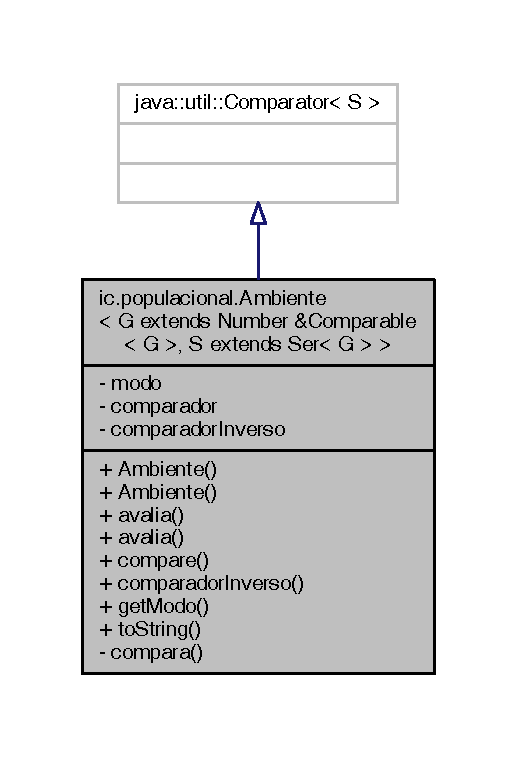
\includegraphics[width=248pt]{classic_1_1populacional_1_1_ambiente_3_01_g_01extends_01_number_01_6_comparable_3_01_g_01_4_00_0ebf80ca98eaa190106331a45750498ba}
\end{center}
\end{figure}


Diagrama de colaboração para ic.\-populacional.\-Ambiente$<$ G extends Number \&Comparable$<$ G $>$, S extends Ser$<$ G $>$ $>$\-:
\nopagebreak
\begin{figure}[H]
\begin{center}
\leavevmode
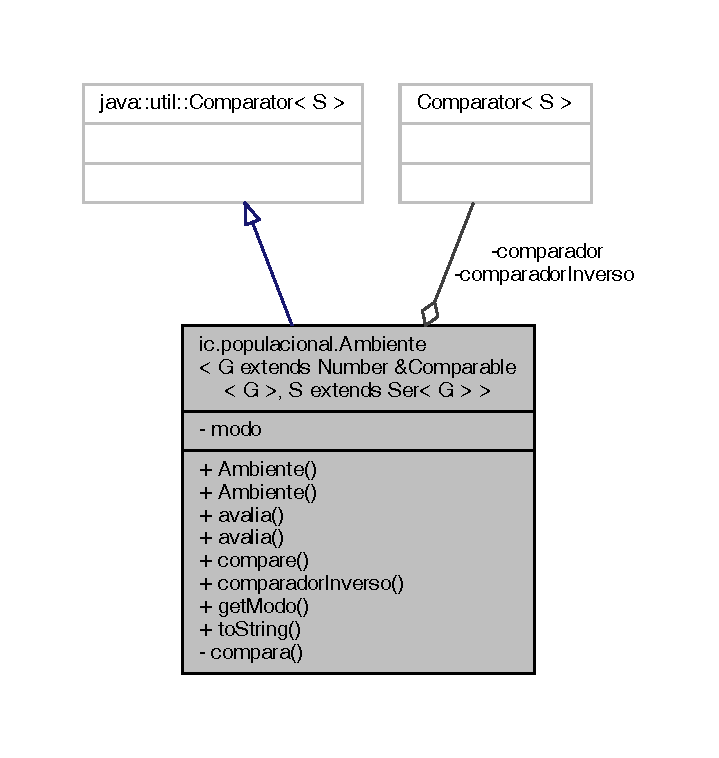
\includegraphics[width=345pt]{classic_1_1populacional_1_1_ambiente_3_01_g_01extends_01_number_01_6_comparable_3_01_g_01_4_00_0eeae7a3fbda8cfca961f3b7ed4d11e09}
\end{center}
\end{figure}
\subsection*{Componentes}
\begin{DoxyCompactItemize}
\item 
enum \hyperlink{enumic_1_1populacional_1_1_ambiente_3_01_g_01extends_01_number_01_6_comparable_3_01_g_01_4_00_0156fb2ffb0f78f5b655aaee5b0df471a7}{Modo}
\begin{DoxyCompactList}\small\item\em Defini o modo de comparação entre os seres. \end{DoxyCompactList}\end{DoxyCompactItemize}
\subsection*{Métodos Públicos}
\begin{DoxyCompactItemize}
\item 
\hyperlink{classic_1_1populacional_1_1_ambiente_3_01_g_01extends_01_number_01_6_comparable_3_01_g_01_4_00_01a5eb548f12ccc7dbff4cf5c498ddc51_ab798f4891bf5d913966cbc68e646c58f}{Ambiente} ()
\begin{DoxyCompactList}\small\item\em Construtor padrão\-: modo Maximização. \end{DoxyCompactList}\item 
\hyperlink{classic_1_1populacional_1_1_ambiente_3_01_g_01extends_01_number_01_6_comparable_3_01_g_01_4_00_01a5eb548f12ccc7dbff4cf5c498ddc51_aeedc08aac80259e2ff6f4524db8b5e07}{Ambiente} (Modo \hyperlink{classic_1_1populacional_1_1_ambiente_3_01_g_01extends_01_number_01_6_comparable_3_01_g_01_4_00_01a5eb548f12ccc7dbff4cf5c498ddc51_afdf6b3d04203015a78f9af1012306dff}{modo})
\begin{DoxyCompactList}\small\item\em Construtor com definição do modo. \end{DoxyCompactList}\item 
abstract G \hyperlink{classic_1_1populacional_1_1_ambiente_3_01_g_01extends_01_number_01_6_comparable_3_01_g_01_4_00_01a5eb548f12ccc7dbff4cf5c498ddc51_a77f4aed5f08c0c4cb6c74e15d9dc1c09}{avalia} (S individuo)
\begin{DoxyCompactList}\small\item\em Função de Fitness\-: Avalia um ser atribuindo um grau de adaptação. \end{DoxyCompactList}\item 
void \hyperlink{classic_1_1populacional_1_1_ambiente_3_01_g_01extends_01_number_01_6_comparable_3_01_g_01_4_00_01a5eb548f12ccc7dbff4cf5c498ddc51_aee3978452491ee78175d4679c2ffebd9}{avalia} (Collection$<$?extends S $>$ seres)
\begin{DoxyCompactList}\small\item\em Avalia uma coleção de seres. \end{DoxyCompactList}\item 
int \hyperlink{classic_1_1populacional_1_1_ambiente_3_01_g_01extends_01_number_01_6_comparable_3_01_g_01_4_00_01a5eb548f12ccc7dbff4cf5c498ddc51_af607dd2a04def8b6ad98835ce5f718d3}{compare} (S ser1, S ser2)
\begin{DoxyCompactList}\small\item\em Compara graus de adaptação. \end{DoxyCompactList}\item 
Comparator$<$ S $>$ \hyperlink{classic_1_1populacional_1_1_ambiente_3_01_g_01extends_01_number_01_6_comparable_3_01_g_01_4_00_01a5eb548f12ccc7dbff4cf5c498ddc51_a90bc2c36b5d705af35821fb38438021e}{comparador\-Inverso} ()
\begin{DoxyCompactList}\small\item\em Retorna um comparador para a ordem invertida quanto ao grau de adaptação. \end{DoxyCompactList}\item 
Modo \hyperlink{classic_1_1populacional_1_1_ambiente_3_01_g_01extends_01_number_01_6_comparable_3_01_g_01_4_00_01a5eb548f12ccc7dbff4cf5c498ddc51_afeaac1bdf13bcc0e889c5241143a438a}{get\-Modo} ()
\begin{DoxyCompactList}\small\item\em Acesso ao modo de comparação. \end{DoxyCompactList}\item 
String \hyperlink{classic_1_1populacional_1_1_ambiente_3_01_g_01extends_01_number_01_6_comparable_3_01_g_01_4_00_01a5eb548f12ccc7dbff4cf5c498ddc51_a1ddc18e33c1028fbbb605a72c3ad09f9}{to\-String} (Populacao populacao)
\begin{DoxyCompactList}\small\item\em Método de para compilação de dados de uma população em formato de string. \end{DoxyCompactList}\end{DoxyCompactItemize}
\subsection*{Métodos Privados}
\begin{DoxyCompactItemize}
\item 
int \hyperlink{classic_1_1populacional_1_1_ambiente_3_01_g_01extends_01_number_01_6_comparable_3_01_g_01_4_00_01a5eb548f12ccc7dbff4cf5c498ddc51_a9a4b847a280696edb0b9c44d2842392f}{compara} (S ser1, S ser2)
\begin{DoxyCompactList}\small\item\em Compara graus de adaptação\-: na ordem crescente. \end{DoxyCompactList}\end{DoxyCompactItemize}
\subsection*{Atributos Privados}
\begin{DoxyCompactItemize}
\item 
final Modo \hyperlink{classic_1_1populacional_1_1_ambiente_3_01_g_01extends_01_number_01_6_comparable_3_01_g_01_4_00_01a5eb548f12ccc7dbff4cf5c498ddc51_afdf6b3d04203015a78f9af1012306dff}{modo}
\item 
final Comparator$<$ S $>$ \hyperlink{classic_1_1populacional_1_1_ambiente_3_01_g_01extends_01_number_01_6_comparable_3_01_g_01_4_00_01a5eb548f12ccc7dbff4cf5c498ddc51_a76dbc9443f7efdba715adc9a0a712f87}{comparador}
\item 
final Comparator$<$ S $>$ \hyperlink{classic_1_1populacional_1_1_ambiente_3_01_g_01extends_01_number_01_6_comparable_3_01_g_01_4_00_01a5eb548f12ccc7dbff4cf5c498ddc51_ab66eaa46861ca2350fd604f36a1a6834}{comparador\-Inverso}
\end{DoxyCompactItemize}


\subsection{Descrição Detalhada}
Essa classe visa criar uma abstração do conceito de ambiente em seu sentido biológico -\/ aplicado a problemas de C\-E. 

Sendo dessa forma, uma entidade avaliadora para uma população, que quando sujeita aos vários fenômenos ambientais, evoluirá no tempo. 

Um ambiente conterá mecanismos que permitirão uma população a evoluir em acordo com as pressões evolutivas impostas, implementadas na forma de métodos em classes mais especializadas – Operadores-\/ que a utilizaram para avaliar soluções geradas. 

De forma generalizada, derivações de {\ttfamily Ambiente} avaliarão indivíduos em uma População, parametrizando seu percurso evolucionário ao atribuir um grau de adaptação a cada um e provendo objetos da classe {\ttfamily Comparator}, capazes de comprar seres em uma ordem crescente ou decrescente em relação ao grau de adaptação. 

\paragraph*{Observação sobre populações\-:}

A classe foi implementada como genérica para garantir a existência de seres (instâncias de classes derivadas de {\ttfamily Ser}) de um único tipo; uma única classe, e suas derivadas, serão usadas em uma população. Deste modo, interpreta-\/se que seres de uma única espécie, e suas subespécies, conviverão em uma população. 

\paragraph*{Suposições básicas\-:}


\begin{DoxyItemize}
\item Seres de uma população pertencem a uma única família de classes derivadas hierarquicamente de {\ttfamily Ser}; mantendo, portanto, a característica de espécie. 
\item Uma população não pode se auto avaliar, bem como seus indivíduos. Uma vez que indivíduos terão um grau de adaptação variado, flutuante, em função do ambiente em que se encontrarão.  
\end{DoxyItemize}

\paragraph*{Responsabilidades\-:}


\begin{DoxyItemize}
\item Avaliar seres; 
\item Avaliar populações(ou coleções de seres); 
\item Comparar seres em relação ao grau de adaptação. 
\end{DoxyItemize}

\begin{DoxyAuthor}{Autor}
Victor de Lima Soares 
\end{DoxyAuthor}
\begin{DoxyVersion}{Versão}
1.\-0
\end{DoxyVersion}

\begin{DoxyParams}{Parâmetros}
{\em $<$\-G$>$} & Classe do retorno da função objetivo (Grau de adaptação)\-: Atomic\-Integer, Atomic\-Long, Big\-Decimal, Big\-Integer, Byte, Double, Float, Integer, Long, Short. \\
\hline
{\em $<$\-S$>$} & Classe dos Seres.\\
\hline
\end{DoxyParams}
\begin{DoxySeeAlso}{Veja também}
Ser 

Populacao 
\end{DoxySeeAlso}


\subsection{Construtores \& Destrutores}
\hypertarget{classic_1_1populacional_1_1_ambiente_3_01_g_01extends_01_number_01_6_comparable_3_01_g_01_4_00_01a5eb548f12ccc7dbff4cf5c498ddc51_ab798f4891bf5d913966cbc68e646c58f}{\index{ic\-::populacional\-::\-Ambiente$<$ G extends Number \&\-Comparable$<$ G $>$, S extends Ser$<$ G $>$ $>$@{ic\-::populacional\-::\-Ambiente$<$ G extends Number \&\-Comparable$<$ G $>$, S extends Ser$<$ G $>$ $>$}!Ambiente@{Ambiente}}
\index{Ambiente@{Ambiente}!ic::populacional::Ambiente< G extends Number &Comparable< G >, S extends Ser< G > >@{ic\-::populacional\-::\-Ambiente$<$ G extends Number \&\-Comparable$<$ G $>$, S extends Ser$<$ G $>$ $>$}}
\subsubsection[{Ambiente}]{\setlength{\rightskip}{0pt plus 5cm}ic.\-populacional.\-Ambiente$<$ G extends Number \&Comparable$<$ G $>$, S extends Ser$<$ G $>$ $>$.Ambiente (
\begin{DoxyParamCaption}
{}
\end{DoxyParamCaption}
)}}\label{classic_1_1populacional_1_1_ambiente_3_01_g_01extends_01_number_01_6_comparable_3_01_g_01_4_00_01a5eb548f12ccc7dbff4cf5c498ddc51_ab798f4891bf5d913966cbc68e646c58f}


Construtor padrão\-: modo Maximização. 

\begin{DoxySince}{Desde}
1.\-0 
\end{DoxySince}
\hypertarget{classic_1_1populacional_1_1_ambiente_3_01_g_01extends_01_number_01_6_comparable_3_01_g_01_4_00_01a5eb548f12ccc7dbff4cf5c498ddc51_aeedc08aac80259e2ff6f4524db8b5e07}{\index{ic\-::populacional\-::\-Ambiente$<$ G extends Number \&\-Comparable$<$ G $>$, S extends Ser$<$ G $>$ $>$@{ic\-::populacional\-::\-Ambiente$<$ G extends Number \&\-Comparable$<$ G $>$, S extends Ser$<$ G $>$ $>$}!Ambiente@{Ambiente}}
\index{Ambiente@{Ambiente}!ic::populacional::Ambiente< G extends Number &Comparable< G >, S extends Ser< G > >@{ic\-::populacional\-::\-Ambiente$<$ G extends Number \&\-Comparable$<$ G $>$, S extends Ser$<$ G $>$ $>$}}
\subsubsection[{Ambiente}]{\setlength{\rightskip}{0pt plus 5cm}ic.\-populacional.\-Ambiente$<$ G extends Number \&Comparable$<$ G $>$, S extends Ser$<$ G $>$ $>$.Ambiente (
\begin{DoxyParamCaption}
\item[{Modo}]{modo}
\end{DoxyParamCaption}
)}}\label{classic_1_1populacional_1_1_ambiente_3_01_g_01extends_01_number_01_6_comparable_3_01_g_01_4_00_01a5eb548f12ccc7dbff4cf5c498ddc51_aeedc08aac80259e2ff6f4524db8b5e07}


Construtor com definição do modo. 

\begin{DoxySince}{Desde}
1.\-0 
\end{DoxySince}

\begin{DoxyParams}{Parâmetros}
{\em modo} & \hyperlink{enumic_1_1populacional_1_1_ambiente_3_01_g_01extends_01_number_01_6_comparable_3_01_g_01_4_00_0156fb2ffb0f78f5b655aaee5b0df471a7}{Modo} de comparação\-: Maximixação/\-Minimização. \\
\hline
\end{DoxyParams}


\subsection{Métodos}
\hypertarget{classic_1_1populacional_1_1_ambiente_3_01_g_01extends_01_number_01_6_comparable_3_01_g_01_4_00_01a5eb548f12ccc7dbff4cf5c498ddc51_a77f4aed5f08c0c4cb6c74e15d9dc1c09}{\index{ic\-::populacional\-::\-Ambiente$<$ G extends Number \&\-Comparable$<$ G $>$, S extends Ser$<$ G $>$ $>$@{ic\-::populacional\-::\-Ambiente$<$ G extends Number \&\-Comparable$<$ G $>$, S extends Ser$<$ G $>$ $>$}!avalia@{avalia}}
\index{avalia@{avalia}!ic::populacional::Ambiente< G extends Number &Comparable< G >, S extends Ser< G > >@{ic\-::populacional\-::\-Ambiente$<$ G extends Number \&\-Comparable$<$ G $>$, S extends Ser$<$ G $>$ $>$}}
\subsubsection[{avalia}]{\setlength{\rightskip}{0pt plus 5cm}abstract G ic.\-populacional.\-Ambiente$<$ G extends Number \&Comparable$<$ G $>$, S extends Ser$<$ G $>$ $>$.avalia (
\begin{DoxyParamCaption}
\item[{S}]{individuo}
\end{DoxyParamCaption}
)\hspace{0.3cm}{\ttfamily [abstract]}}}\label{classic_1_1populacional_1_1_ambiente_3_01_g_01extends_01_number_01_6_comparable_3_01_g_01_4_00_01a5eb548f12ccc7dbff4cf5c498ddc51_a77f4aed5f08c0c4cb6c74e15d9dc1c09}


Função de Fitness\-: Avalia um ser atribuindo um grau de adaptação. 

Atua como função objetivo em algoritmos de otimização e permite que seres sejam classificados em função do seu grau de adaptação, nesse ambiente. 

Essa função {\bfseries deve chamar} \hyperlink{}{Ser\#set\-Grau\-De\-Adaptacao(java.\-lang.\-Number\&java.\-lang.\-Comparable$<$\-G$>$)} uma vez que seu valor de retorno for calculado para que o mesmo seja retido -\/ se essa for a intenção. Essa pode ser chamada após o retorno,contudo. 

\begin{DoxySince}{Desde}
1.\-0 
\end{DoxySince}

\begin{DoxyParams}{Parâmetros}
{\em individuo} & Ser a ser avaliado. \\
\hline
\end{DoxyParams}
\begin{DoxyReturn}{Retorna}
Grau de adaptação.
\end{DoxyReturn}
\begin{DoxySeeAlso}{Veja também}
Ser\-::set\-Grau\-De\-Adaptacao(java.\-lang.\-Number\&java.\-lang.\-Comparable$<$\-G$>$) 
\end{DoxySeeAlso}
\hypertarget{classic_1_1populacional_1_1_ambiente_3_01_g_01extends_01_number_01_6_comparable_3_01_g_01_4_00_01a5eb548f12ccc7dbff4cf5c498ddc51_aee3978452491ee78175d4679c2ffebd9}{\index{ic\-::populacional\-::\-Ambiente$<$ G extends Number \&\-Comparable$<$ G $>$, S extends Ser$<$ G $>$ $>$@{ic\-::populacional\-::\-Ambiente$<$ G extends Number \&\-Comparable$<$ G $>$, S extends Ser$<$ G $>$ $>$}!avalia@{avalia}}
\index{avalia@{avalia}!ic::populacional::Ambiente< G extends Number &Comparable< G >, S extends Ser< G > >@{ic\-::populacional\-::\-Ambiente$<$ G extends Number \&\-Comparable$<$ G $>$, S extends Ser$<$ G $>$ $>$}}
\subsubsection[{avalia}]{\setlength{\rightskip}{0pt plus 5cm}void ic.\-populacional.\-Ambiente$<$ G extends Number \&Comparable$<$ G $>$, S extends Ser$<$ G $>$ $>$.avalia (
\begin{DoxyParamCaption}
\item[{Collection$<$?extends S $>$}]{seres}
\end{DoxyParamCaption}
)}}\label{classic_1_1populacional_1_1_ambiente_3_01_g_01extends_01_number_01_6_comparable_3_01_g_01_4_00_01a5eb548f12ccc7dbff4cf5c498ddc51_aee3978452491ee78175d4679c2ffebd9}


Avalia uma coleção de seres. 

Avalia uma coleção de seres pela chamada repetitiva de \hyperlink{}{avalia(ic.\-populacional.\-Ser)}. 

Por questões de desempenho, considera-\/se que \hyperlink{}{avalia(ic.\-populacional.\-Ser)} constitua-\/se de uma função cujo tempo computacional para execução seja elevado. Portanto, a coleção é usada para a geração de uma stream paralelizada, onde múltiplas threads são criadas para avaliar os seres individualmente. 

Essa função atribui a cada ser na coleção um grau de adaptação por meio da função\-: \hyperlink{}{Ser\#set\-Grau\-De\-Adaptacao(java.\-lang.\-Number\&java.\-lang.\-Comparable$<$\-G$>$)} 

\begin{DoxySince}{Desde}
1.\-0 
\end{DoxySince}

\begin{DoxyParams}{Parâmetros}
{\em seres} & Coleção a ser avaliada.\\
\hline
\end{DoxyParams}
\begin{DoxySeeAlso}{Veja também}
\hyperlink{classic_1_1populacional_1_1_ambiente_3_01_g_01extends_01_number_01_6_comparable_3_01_g_01_4_00_01a5eb548f12ccc7dbff4cf5c498ddc51_a77f4aed5f08c0c4cb6c74e15d9dc1c09}{avalia}(ic.\-populacional.\-Ser) 

Ser\-::set\-Grau\-De\-Adaptacao(java.\-lang.\-Number\&java.\-lang.\-Comparable$<$\-G$>$) 
\end{DoxySeeAlso}
\hypertarget{classic_1_1populacional_1_1_ambiente_3_01_g_01extends_01_number_01_6_comparable_3_01_g_01_4_00_01a5eb548f12ccc7dbff4cf5c498ddc51_a9a4b847a280696edb0b9c44d2842392f}{\index{ic\-::populacional\-::\-Ambiente$<$ G extends Number \&\-Comparable$<$ G $>$, S extends Ser$<$ G $>$ $>$@{ic\-::populacional\-::\-Ambiente$<$ G extends Number \&\-Comparable$<$ G $>$, S extends Ser$<$ G $>$ $>$}!compara@{compara}}
\index{compara@{compara}!ic::populacional::Ambiente< G extends Number &Comparable< G >, S extends Ser< G > >@{ic\-::populacional\-::\-Ambiente$<$ G extends Number \&\-Comparable$<$ G $>$, S extends Ser$<$ G $>$ $>$}}
\subsubsection[{compara}]{\setlength{\rightskip}{0pt plus 5cm}int ic.\-populacional.\-Ambiente$<$ G extends Number \&Comparable$<$ G $>$, S extends Ser$<$ G $>$ $>$.compara (
\begin{DoxyParamCaption}
\item[{S}]{ser1, }
\item[{S}]{ser2}
\end{DoxyParamCaption}
)\hspace{0.3cm}{\ttfamily [private]}}}\label{classic_1_1populacional_1_1_ambiente_3_01_g_01extends_01_number_01_6_comparable_3_01_g_01_4_00_01a5eb548f12ccc7dbff4cf5c498ddc51_a9a4b847a280696edb0b9c44d2842392f}


Compara graus de adaptação\-: na ordem crescente. 

Compara dois seres, possibilitando sua ordenação quanto a adaptação. 


\begin{DoxyParams}{Parâmetros}
{\em ser1} & Ser a ser comparado pelo ambiente. \\
\hline
{\em ser2} & Segundo Ser a ser comparado pelo ambiente.\\
\hline
\end{DoxyParams}
\begin{DoxyReturn}{Retorna}

\begin{DoxyItemize}
\item Positivo se ser1 for melhor adptado. 
\item Negativo se ser2 for melhor adptado. 
\item 0 se forem igualmente adaptados. 
\end{DoxyItemize}
\end{DoxyReturn}
\begin{DoxySince}{Desde}
1.\-0
\end{DoxySince}
\begin{DoxySeeAlso}{Veja também}
Comparable\-::compare\-To(java.\-lang.\-Object) 
\end{DoxySeeAlso}
\hypertarget{classic_1_1populacional_1_1_ambiente_3_01_g_01extends_01_number_01_6_comparable_3_01_g_01_4_00_01a5eb548f12ccc7dbff4cf5c498ddc51_a90bc2c36b5d705af35821fb38438021e}{\index{ic\-::populacional\-::\-Ambiente$<$ G extends Number \&\-Comparable$<$ G $>$, S extends Ser$<$ G $>$ $>$@{ic\-::populacional\-::\-Ambiente$<$ G extends Number \&\-Comparable$<$ G $>$, S extends Ser$<$ G $>$ $>$}!comparador\-Inverso@{comparador\-Inverso}}
\index{comparador\-Inverso@{comparador\-Inverso}!ic::populacional::Ambiente< G extends Number &Comparable< G >, S extends Ser< G > >@{ic\-::populacional\-::\-Ambiente$<$ G extends Number \&\-Comparable$<$ G $>$, S extends Ser$<$ G $>$ $>$}}
\subsubsection[{comparador\-Inverso}]{\setlength{\rightskip}{0pt plus 5cm}Comparator$<$S$>$ ic.\-populacional.\-Ambiente$<$ G extends Number \&Comparable$<$ G $>$, S extends Ser$<$ G $>$ $>$.comparador\-Inverso (
\begin{DoxyParamCaption}
{}
\end{DoxyParamCaption}
)}}\label{classic_1_1populacional_1_1_ambiente_3_01_g_01extends_01_number_01_6_comparable_3_01_g_01_4_00_01a5eb548f12ccc7dbff4cf5c498ddc51_a90bc2c36b5d705af35821fb38438021e}


Retorna um comparador para a ordem invertida quanto ao grau de adaptação. 

\begin{DoxySince}{Desde}
1.\-0 
\end{DoxySince}
\begin{DoxyReturn}{Retorna}
Comparator para ordem invertida.
\end{DoxyReturn}
\begin{DoxySeeAlso}{Veja também}
Comparable\-::compare\-To(java.\-lang.\-Object) 
\end{DoxySeeAlso}
\hypertarget{classic_1_1populacional_1_1_ambiente_3_01_g_01extends_01_number_01_6_comparable_3_01_g_01_4_00_01a5eb548f12ccc7dbff4cf5c498ddc51_af607dd2a04def8b6ad98835ce5f718d3}{\index{ic\-::populacional\-::\-Ambiente$<$ G extends Number \&\-Comparable$<$ G $>$, S extends Ser$<$ G $>$ $>$@{ic\-::populacional\-::\-Ambiente$<$ G extends Number \&\-Comparable$<$ G $>$, S extends Ser$<$ G $>$ $>$}!compare@{compare}}
\index{compare@{compare}!ic::populacional::Ambiente< G extends Number &Comparable< G >, S extends Ser< G > >@{ic\-::populacional\-::\-Ambiente$<$ G extends Number \&\-Comparable$<$ G $>$, S extends Ser$<$ G $>$ $>$}}
\subsubsection[{compare}]{\setlength{\rightskip}{0pt plus 5cm}int ic.\-populacional.\-Ambiente$<$ G extends Number \&Comparable$<$ G $>$, S extends Ser$<$ G $>$ $>$.compare (
\begin{DoxyParamCaption}
\item[{S}]{ser1, }
\item[{S}]{ser2}
\end{DoxyParamCaption}
)}}\label{classic_1_1populacional_1_1_ambiente_3_01_g_01extends_01_number_01_6_comparable_3_01_g_01_4_00_01a5eb548f12ccc7dbff4cf5c498ddc51_af607dd2a04def8b6ad98835ce5f718d3}


Compara graus de adaptação. 

Compara dois seres, possibilitando sua ordenação quanto a adaptação. 


\begin{DoxyParams}{Parâmetros}
{\em ser1} & Ser a ser comparado pelo ambiente. \\
\hline
{\em ser2} & Segundo Ser a ser comparado pelo ambiente.\\
\hline
\end{DoxyParams}
\begin{DoxyReturn}{Retorna}

\begin{DoxyItemize}
\item Positivo se ser1 for melhor adptado. 
\item Negativo se ser2 for melhor adptado. 
\item 0 se forem igualmente adaptados. 
\end{DoxyItemize}
\end{DoxyReturn}
\begin{DoxySince}{Desde}
1.\-0
\end{DoxySince}
\begin{DoxySeeAlso}{Veja também}
Comparable\-::compare\-To(java.\-lang.\-Object) 
\end{DoxySeeAlso}
\hypertarget{classic_1_1populacional_1_1_ambiente_3_01_g_01extends_01_number_01_6_comparable_3_01_g_01_4_00_01a5eb548f12ccc7dbff4cf5c498ddc51_afeaac1bdf13bcc0e889c5241143a438a}{\index{ic\-::populacional\-::\-Ambiente$<$ G extends Number \&\-Comparable$<$ G $>$, S extends Ser$<$ G $>$ $>$@{ic\-::populacional\-::\-Ambiente$<$ G extends Number \&\-Comparable$<$ G $>$, S extends Ser$<$ G $>$ $>$}!get\-Modo@{get\-Modo}}
\index{get\-Modo@{get\-Modo}!ic::populacional::Ambiente< G extends Number &Comparable< G >, S extends Ser< G > >@{ic\-::populacional\-::\-Ambiente$<$ G extends Number \&\-Comparable$<$ G $>$, S extends Ser$<$ G $>$ $>$}}
\subsubsection[{get\-Modo}]{\setlength{\rightskip}{0pt plus 5cm}Modo ic.\-populacional.\-Ambiente$<$ G extends Number \&Comparable$<$ G $>$, S extends Ser$<$ G $>$ $>$.get\-Modo (
\begin{DoxyParamCaption}
{}
\end{DoxyParamCaption}
)}}\label{classic_1_1populacional_1_1_ambiente_3_01_g_01extends_01_number_01_6_comparable_3_01_g_01_4_00_01a5eb548f12ccc7dbff4cf5c498ddc51_afeaac1bdf13bcc0e889c5241143a438a}


Acesso ao modo de comparação. 

\begin{DoxySince}{Desde}
1.\-0 
\end{DoxySince}
\begin{DoxyReturn}{Retorna}
\hyperlink{enumic_1_1populacional_1_1_ambiente_3_01_g_01extends_01_number_01_6_comparable_3_01_g_01_4_00_0156fb2ffb0f78f5b655aaee5b0df471a7}{Modo} de comparação. 
\end{DoxyReturn}
\hypertarget{classic_1_1populacional_1_1_ambiente_3_01_g_01extends_01_number_01_6_comparable_3_01_g_01_4_00_01a5eb548f12ccc7dbff4cf5c498ddc51_a1ddc18e33c1028fbbb605a72c3ad09f9}{\index{ic\-::populacional\-::\-Ambiente$<$ G extends Number \&\-Comparable$<$ G $>$, S extends Ser$<$ G $>$ $>$@{ic\-::populacional\-::\-Ambiente$<$ G extends Number \&\-Comparable$<$ G $>$, S extends Ser$<$ G $>$ $>$}!to\-String@{to\-String}}
\index{to\-String@{to\-String}!ic::populacional::Ambiente< G extends Number &Comparable< G >, S extends Ser< G > >@{ic\-::populacional\-::\-Ambiente$<$ G extends Number \&\-Comparable$<$ G $>$, S extends Ser$<$ G $>$ $>$}}
\subsubsection[{to\-String}]{\setlength{\rightskip}{0pt plus 5cm}String ic.\-populacional.\-Ambiente$<$ G extends Number \&Comparable$<$ G $>$, S extends Ser$<$ G $>$ $>$.to\-String (
\begin{DoxyParamCaption}
\item[{Populacao}]{populacao}
\end{DoxyParamCaption}
)}}\label{classic_1_1populacional_1_1_ambiente_3_01_g_01extends_01_number_01_6_comparable_3_01_g_01_4_00_01a5eb548f12ccc7dbff4cf5c498ddc51_a1ddc18e33c1028fbbb605a72c3ad09f9}


Método de para compilação de dados de uma população em formato de string. 

\begin{DoxySince}{Desde}
1.\-0 
\end{DoxySince}

\begin{DoxyParams}{Parâmetros}
{\em populacao} & \\
\hline
\end{DoxyParams}
\begin{DoxyReturn}{Retorna}
String com dados da população.
\end{DoxyReturn}
\begin{DoxyRefDesc}{Descontinuado(a)}
\item[\hyperlink{deprecated__deprecated000001}{Descontinuado(a)}]\begin{DoxySeeAlso}{Veja também}
Populacao\-::to\-String() 
\end{DoxySeeAlso}
\end{DoxyRefDesc}


\subsection{Atributos}
\hypertarget{classic_1_1populacional_1_1_ambiente_3_01_g_01extends_01_number_01_6_comparable_3_01_g_01_4_00_01a5eb548f12ccc7dbff4cf5c498ddc51_a76dbc9443f7efdba715adc9a0a712f87}{\index{ic\-::populacional\-::\-Ambiente$<$ G extends Number \&\-Comparable$<$ G $>$, S extends Ser$<$ G $>$ $>$@{ic\-::populacional\-::\-Ambiente$<$ G extends Number \&\-Comparable$<$ G $>$, S extends Ser$<$ G $>$ $>$}!comparador@{comparador}}
\index{comparador@{comparador}!ic::populacional::Ambiente< G extends Number &Comparable< G >, S extends Ser< G > >@{ic\-::populacional\-::\-Ambiente$<$ G extends Number \&\-Comparable$<$ G $>$, S extends Ser$<$ G $>$ $>$}}
\subsubsection[{comparador}]{\setlength{\rightskip}{0pt plus 5cm}final Comparator$<$S$>$ ic.\-populacional.\-Ambiente$<$ G extends Number \&Comparable$<$ G $>$, S extends Ser$<$ G $>$ $>$.comparador\hspace{0.3cm}{\ttfamily [private]}}}\label{classic_1_1populacional_1_1_ambiente_3_01_g_01extends_01_number_01_6_comparable_3_01_g_01_4_00_01a5eb548f12ccc7dbff4cf5c498ddc51_a76dbc9443f7efdba715adc9a0a712f87}
\hypertarget{classic_1_1populacional_1_1_ambiente_3_01_g_01extends_01_number_01_6_comparable_3_01_g_01_4_00_01a5eb548f12ccc7dbff4cf5c498ddc51_ab66eaa46861ca2350fd604f36a1a6834}{\index{ic\-::populacional\-::\-Ambiente$<$ G extends Number \&\-Comparable$<$ G $>$, S extends Ser$<$ G $>$ $>$@{ic\-::populacional\-::\-Ambiente$<$ G extends Number \&\-Comparable$<$ G $>$, S extends Ser$<$ G $>$ $>$}!comparador\-Inverso@{comparador\-Inverso}}
\index{comparador\-Inverso@{comparador\-Inverso}!ic::populacional::Ambiente< G extends Number &Comparable< G >, S extends Ser< G > >@{ic\-::populacional\-::\-Ambiente$<$ G extends Number \&\-Comparable$<$ G $>$, S extends Ser$<$ G $>$ $>$}}
\subsubsection[{comparador\-Inverso}]{\setlength{\rightskip}{0pt plus 5cm}final Comparator$<$S$>$ ic.\-populacional.\-Ambiente$<$ G extends Number \&Comparable$<$ G $>$, S extends Ser$<$ G $>$ $>$.comparador\-Inverso\hspace{0.3cm}{\ttfamily [private]}}}\label{classic_1_1populacional_1_1_ambiente_3_01_g_01extends_01_number_01_6_comparable_3_01_g_01_4_00_01a5eb548f12ccc7dbff4cf5c498ddc51_ab66eaa46861ca2350fd604f36a1a6834}
\hypertarget{classic_1_1populacional_1_1_ambiente_3_01_g_01extends_01_number_01_6_comparable_3_01_g_01_4_00_01a5eb548f12ccc7dbff4cf5c498ddc51_afdf6b3d04203015a78f9af1012306dff}{\index{ic\-::populacional\-::\-Ambiente$<$ G extends Number \&\-Comparable$<$ G $>$, S extends Ser$<$ G $>$ $>$@{ic\-::populacional\-::\-Ambiente$<$ G extends Number \&\-Comparable$<$ G $>$, S extends Ser$<$ G $>$ $>$}!modo@{modo}}
\index{modo@{modo}!ic::populacional::Ambiente< G extends Number &Comparable< G >, S extends Ser< G > >@{ic\-::populacional\-::\-Ambiente$<$ G extends Number \&\-Comparable$<$ G $>$, S extends Ser$<$ G $>$ $>$}}
\subsubsection[{modo}]{\setlength{\rightskip}{0pt plus 5cm}final Modo ic.\-populacional.\-Ambiente$<$ G extends Number \&Comparable$<$ G $>$, S extends Ser$<$ G $>$ $>$.modo\hspace{0.3cm}{\ttfamily [private]}}}\label{classic_1_1populacional_1_1_ambiente_3_01_g_01extends_01_number_01_6_comparable_3_01_g_01_4_00_01a5eb548f12ccc7dbff4cf5c498ddc51_afdf6b3d04203015a78f9af1012306dff}


A documentação para esta classe foi gerada a partir do seguinte arquivo\-:\begin{DoxyCompactItemize}
\item 
C\-:/\-Users/\-Victor/workplace/\-Net\-Beans\-Projects/\-Inteligencia Computacional/src/ic/populacional/\hyperlink{_ambiente_8java}{Ambiente.\-java}\end{DoxyCompactItemize}

\hypertarget{classic_1_1populacional_1_1utilidades_1_1_binario}{\section{Referência da Classe ic.\-populacional.\-utilidades.\-Binario}
\label{classic_1_1populacional_1_1utilidades_1_1_binario}\index{ic.\-populacional.\-utilidades.\-Binario@{ic.\-populacional.\-utilidades.\-Binario}}
}


Diagrama de colaboração para ic.\-populacional.\-utilidades.\-Binario\-:\nopagebreak
\begin{figure}[H]
\begin{center}
\leavevmode
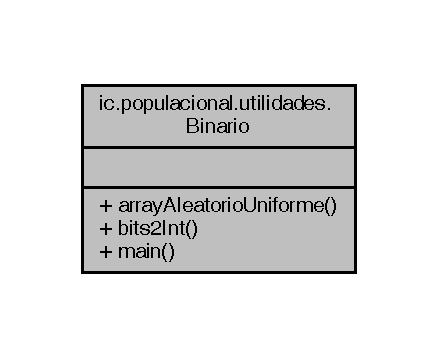
\includegraphics[width=210pt]{classic_1_1populacional_1_1utilidades_1_1_binario__coll__graph}
\end{center}
\end{figure}
\subsection*{Métodos Públicos Estáticos}
\begin{DoxyCompactItemize}
\item 
static final List$<$ Boolean $>$ \hyperlink{classic_1_1populacional_1_1utilidades_1_1_binario_a2ee67758516b8b1a9a3a2def3925f52c}{array\-Aleatorio\-Uniforme} (int nbits)
\begin{DoxyCompactList}\small\item\em Retorna n índices aleatórios em uma permutação de inteiros. \end{DoxyCompactList}\item 
static final int \hyperlink{classic_1_1populacional_1_1utilidades_1_1_binario_acbadb46434856fd58bbe1d9dbfd5447c}{bits2\-Int} (List$<$ Boolean $>$ bits)
\item 
static void \hyperlink{classic_1_1populacional_1_1utilidades_1_1_binario_abd5219bf86018207e870767f7facc6a0}{main} (String...\-args)
\end{DoxyCompactItemize}


\subsection{Descrição Detalhada}
\begin{DoxyAuthor}{Autor}
Victor de Lima Soares 
\end{DoxyAuthor}


\subsection{Métodos}
\hypertarget{classic_1_1populacional_1_1utilidades_1_1_binario_a2ee67758516b8b1a9a3a2def3925f52c}{\index{ic\-::populacional\-::utilidades\-::\-Binario@{ic\-::populacional\-::utilidades\-::\-Binario}!array\-Aleatorio\-Uniforme@{array\-Aleatorio\-Uniforme}}
\index{array\-Aleatorio\-Uniforme@{array\-Aleatorio\-Uniforme}!ic::populacional::utilidades::Binario@{ic\-::populacional\-::utilidades\-::\-Binario}}
\subsubsection[{array\-Aleatorio\-Uniforme}]{\setlength{\rightskip}{0pt plus 5cm}static final List$<$Boolean$>$ ic.\-populacional.\-utilidades.\-Binario.\-array\-Aleatorio\-Uniforme (
\begin{DoxyParamCaption}
\item[{int}]{nbits}
\end{DoxyParamCaption}
)\hspace{0.3cm}{\ttfamily [static]}}}\label{classic_1_1populacional_1_1utilidades_1_1_binario_a2ee67758516b8b1a9a3a2def3925f52c}


Retorna n índices aleatórios em uma permutação de inteiros. 

Distribuição uniforme.

\begin{DoxyReturn}{Retorna}
Índices escolhidos aleatoriamente, sem uma permutação de inteiros. 
\end{DoxyReturn}
\hypertarget{classic_1_1populacional_1_1utilidades_1_1_binario_acbadb46434856fd58bbe1d9dbfd5447c}{\index{ic\-::populacional\-::utilidades\-::\-Binario@{ic\-::populacional\-::utilidades\-::\-Binario}!bits2\-Int@{bits2\-Int}}
\index{bits2\-Int@{bits2\-Int}!ic::populacional::utilidades::Binario@{ic\-::populacional\-::utilidades\-::\-Binario}}
\subsubsection[{bits2\-Int}]{\setlength{\rightskip}{0pt plus 5cm}static final int ic.\-populacional.\-utilidades.\-Binario.\-bits2\-Int (
\begin{DoxyParamCaption}
\item[{List$<$ Boolean $>$}]{bits}
\end{DoxyParamCaption}
)\hspace{0.3cm}{\ttfamily [static]}}}\label{classic_1_1populacional_1_1utilidades_1_1_binario_acbadb46434856fd58bbe1d9dbfd5447c}


Este é o diagrama das funções que utilizam esta função\-:\nopagebreak
\begin{figure}[H]
\begin{center}
\leavevmode
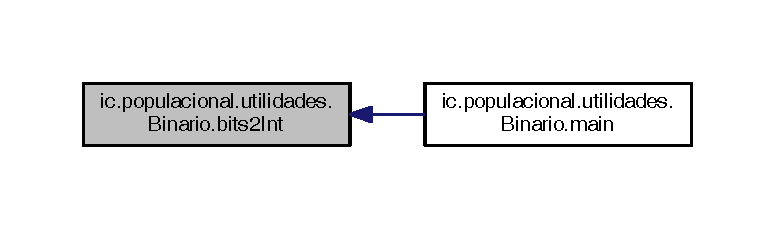
\includegraphics[width=350pt]{classic_1_1populacional_1_1utilidades_1_1_binario_acbadb46434856fd58bbe1d9dbfd5447c_icgraph}
\end{center}
\end{figure}


\hypertarget{classic_1_1populacional_1_1utilidades_1_1_binario_abd5219bf86018207e870767f7facc6a0}{\index{ic\-::populacional\-::utilidades\-::\-Binario@{ic\-::populacional\-::utilidades\-::\-Binario}!main@{main}}
\index{main@{main}!ic::populacional::utilidades::Binario@{ic\-::populacional\-::utilidades\-::\-Binario}}
\subsubsection[{main}]{\setlength{\rightskip}{0pt plus 5cm}static void ic.\-populacional.\-utilidades.\-Binario.\-main (
\begin{DoxyParamCaption}
\item[{String...}]{args}
\end{DoxyParamCaption}
)\hspace{0.3cm}{\ttfamily [static]}}}\label{classic_1_1populacional_1_1utilidades_1_1_binario_abd5219bf86018207e870767f7facc6a0}


Este é o diagrama das funções utilizadas por esta função\-:\nopagebreak
\begin{figure}[H]
\begin{center}
\leavevmode
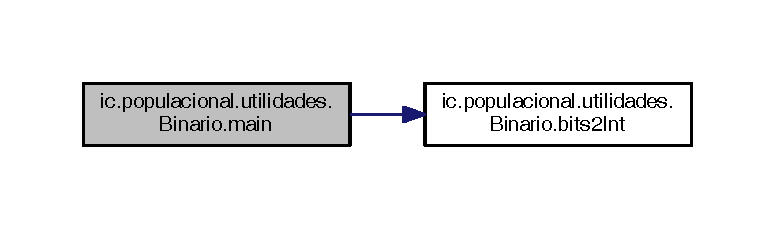
\includegraphics[width=350pt]{classic_1_1populacional_1_1utilidades_1_1_binario_abd5219bf86018207e870767f7facc6a0_cgraph}
\end{center}
\end{figure}




A documentação para esta classe foi gerada a partir do seguinte arquivo\-:\begin{DoxyCompactItemize}
\item 
C\-:/\-Users/\-Victor/workplace/\-Net\-Beans\-Projects/\-Inteligencia Computacional/src/ic/populacional/utilidades/\hyperlink{_binario_8java}{Binario.\-java}\end{DoxyCompactItemize}

\hypertarget{interfaceic_1_1populacional_1_1_caracteristica_3_01_v_01extends_01_number_01_4}{\section{Referência da Interface ic.\-populacional.\-Caracteristica$<$ V extends Number $>$}
\label{interfaceic_1_1populacional_1_1_caracteristica_3_01_v_01extends_01_number_01_4}\index{ic.\-populacional.\-Caracteristica$<$ V extends Number $>$@{ic.\-populacional.\-Caracteristica$<$ V extends Number $>$}}
}


Diagrama de colaboração para ic.\-populacional.\-Caracteristica$<$ V extends Number $>$\-:
\nopagebreak
\begin{figure}[H]
\begin{center}
\leavevmode
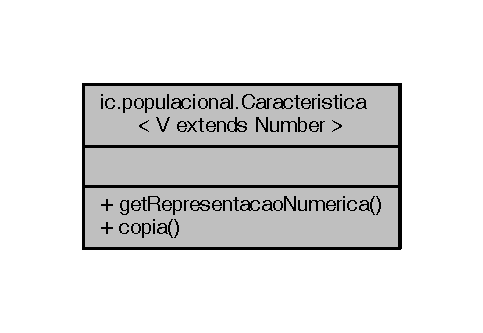
\includegraphics[width=232pt]{interfaceic_1_1populacional_1_1_caracteristica_3_01_v_01extends_01_number_01_4__coll__graph}
\end{center}
\end{figure}
\subsection*{Métodos Públicos}
\begin{DoxyCompactItemize}
\item 
V \hyperlink{interfaceic_1_1populacional_1_1_caracteristica_3_01_v_01extends_01_number_01_4_a974c1c992b4b916c8b92217f2a381ff6}{get\-Representacao\-Numerica} ()
\begin{DoxyCompactList}\small\item\em Calcula uma representação (expressão) numérica para essa característica. \end{DoxyCompactList}\item 
Caracteristica \hyperlink{interfaceic_1_1populacional_1_1_caracteristica_3_01_v_01extends_01_number_01_4_a5c687979e881636769c487450193599b}{copia} ()
\begin{DoxyCompactList}\small\item\em Retorna uma cópia da característica. \end{DoxyCompactList}\end{DoxyCompactItemize}


\subsection{Descrição Detalhada}
\begin{DoxyAuthor}{Autor}
Victor Soares 
\end{DoxyAuthor}
\begin{DoxyVersion}{Versão}
1.\-0
\end{DoxyVersion}

\begin{DoxyParams}{Parâmetros}
{\em $<$\-V$>$} & Tipo da representação numérica da característica. \\
\hline
\end{DoxyParams}


\subsection{Métodos}
\hypertarget{interfaceic_1_1populacional_1_1_caracteristica_3_01_v_01extends_01_number_01_4_a5c687979e881636769c487450193599b}{\index{ic\-::populacional\-::\-Caracteristica$<$ V extends Number $>$@{ic\-::populacional\-::\-Caracteristica$<$ V extends Number $>$}!copia@{copia}}
\index{copia@{copia}!ic::populacional::Caracteristica< V extends Number >@{ic\-::populacional\-::\-Caracteristica$<$ V extends Number $>$}}
\subsubsection[{copia}]{\setlength{\rightskip}{0pt plus 5cm}Caracteristica ic.\-populacional.\-Caracteristica$<$ V extends Number $>$.copia (
\begin{DoxyParamCaption}
{}
\end{DoxyParamCaption}
)}}\label{interfaceic_1_1populacional_1_1_caracteristica_3_01_v_01extends_01_number_01_4_a5c687979e881636769c487450193599b}


Retorna uma cópia da característica. 

Essa cópia deverá ser uma nova instância, tal que {\ttfamily iquals(copia)} seja verdadeiro. Difere de clone, para evitar conflito na A\-P\-I, e resultados inesperados. 

{\bfseries Deve gerar nova instância}

\begin{DoxySeeAlso}{Veja também}
Object\-::equals(java.\-lang.\-Object) 
\end{DoxySeeAlso}
\begin{DoxyReturn}{Retorna}
Uma copia desta característica. 
\end{DoxyReturn}
\hypertarget{interfaceic_1_1populacional_1_1_caracteristica_3_01_v_01extends_01_number_01_4_a974c1c992b4b916c8b92217f2a381ff6}{\index{ic\-::populacional\-::\-Caracteristica$<$ V extends Number $>$@{ic\-::populacional\-::\-Caracteristica$<$ V extends Number $>$}!get\-Representacao\-Numerica@{get\-Representacao\-Numerica}}
\index{get\-Representacao\-Numerica@{get\-Representacao\-Numerica}!ic::populacional::Caracteristica< V extends Number >@{ic\-::populacional\-::\-Caracteristica$<$ V extends Number $>$}}
\subsubsection[{get\-Representacao\-Numerica}]{\setlength{\rightskip}{0pt plus 5cm}V ic.\-populacional.\-Caracteristica$<$ V extends Number $>$.get\-Representacao\-Numerica (
\begin{DoxyParamCaption}
{}
\end{DoxyParamCaption}
)}}\label{interfaceic_1_1populacional_1_1_caracteristica_3_01_v_01extends_01_number_01_4_a974c1c992b4b916c8b92217f2a381ff6}


Calcula uma representação (expressão) numérica para essa característica. 

Características podem conter uma série de informações sobre si mesma, constituindo o globalmente o genótipo dos seres que as contem. Porém, uma expressão numérica única, sumarizando os efeitos mais relevantes dessa unidade de formação do ser em um único número, é necessária tanto para criar-\/se um modelo fenótipo, quanto para propósitos de processamento. 

\begin{DoxySince}{Desde}
1.\-0 
\end{DoxySince}
\begin{DoxyReturn}{Retorna}
Expressão numérica da característica.
\end{DoxyReturn}
\begin{DoxySeeAlso}{Veja também}
Ser 
\end{DoxySeeAlso}


A documentação para esta interface foi gerada a partir do seguinte arquivo\-:\begin{DoxyCompactItemize}
\item 
C\-:/\-Users/\-Victor/workplace/\-Net\-Beans\-Projects/\-Inteligencia Computacional/src/ic/populacional/\hyperlink{_caracteristica_8java}{Caracteristica.\-java}\end{DoxyCompactItemize}

\hypertarget{classic_1_1populacional_1_1seres_1_1binarios_1_1_caracteristica_binaria}{\section{Referência da Classe ic.\-populacional.\-seres.\-binarios.\-Caracteristica\-Binaria}
\label{classic_1_1populacional_1_1seres_1_1binarios_1_1_caracteristica_binaria}\index{ic.\-populacional.\-seres.\-binarios.\-Caracteristica\-Binaria@{ic.\-populacional.\-seres.\-binarios.\-Caracteristica\-Binaria}}
}


Diagrama de Hierarquia para ic.\-populacional.\-seres.\-binarios.\-Caracteristica\-Binaria\-:
\nopagebreak
\begin{figure}[H]
\begin{center}
\leavevmode
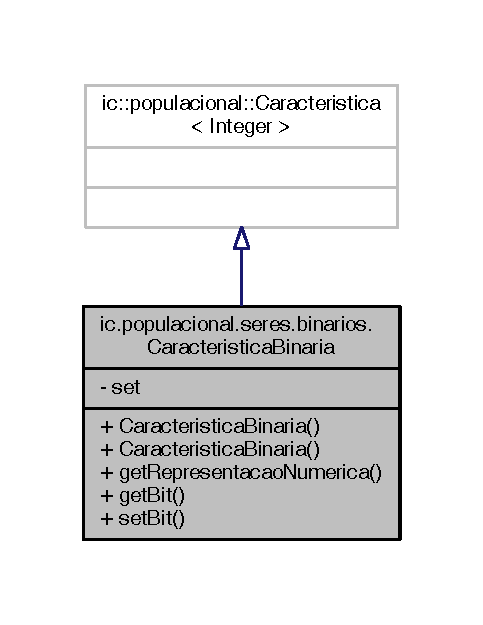
\includegraphics[width=232pt]{classic_1_1populacional_1_1seres_1_1binarios_1_1_caracteristica_binaria__inherit__graph}
\end{center}
\end{figure}


Diagrama de colaboração para ic.\-populacional.\-seres.\-binarios.\-Caracteristica\-Binaria\-:
\nopagebreak
\begin{figure}[H]
\begin{center}
\leavevmode
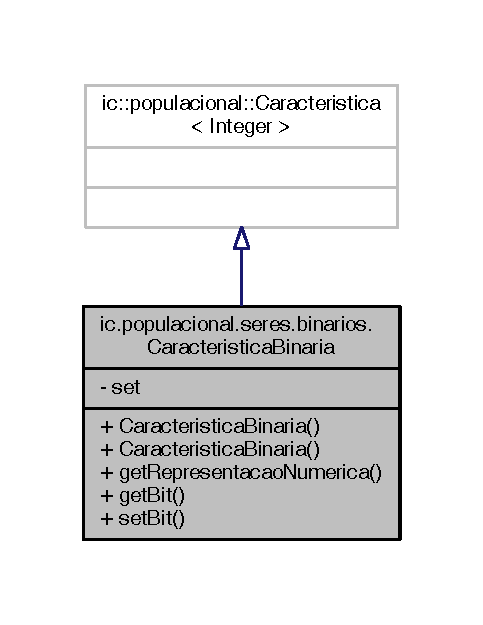
\includegraphics[width=232pt]{classic_1_1populacional_1_1seres_1_1binarios_1_1_caracteristica_binaria__coll__graph}
\end{center}
\end{figure}
\subsection*{Métodos Públicos}
\begin{DoxyCompactItemize}
\item 
\hyperlink{classic_1_1populacional_1_1seres_1_1binarios_1_1_caracteristica_binaria_a56d2bb8f266a6e15df2b6c719ba3a02a}{Caracteristica\-Binaria} ()
\item 
\hyperlink{classic_1_1populacional_1_1seres_1_1binarios_1_1_caracteristica_binaria_a2ec5867b48fcfcdafb5f82fc01be6682}{Caracteristica\-Binaria} (boolean \hyperlink{classic_1_1populacional_1_1seres_1_1binarios_1_1_caracteristica_binaria_a681ee9eb0af3a4e8dfc2f5534602f558}{set})
\item 
Integer \hyperlink{classic_1_1populacional_1_1seres_1_1binarios_1_1_caracteristica_binaria_afc753198f1e3d4bda1b714c5e19498ee}{get\-Representacao\-Numerica} ()
\item 
boolean \hyperlink{classic_1_1populacional_1_1seres_1_1binarios_1_1_caracteristica_binaria_a7c5984e632a36604d8644cde332e266e}{get\-Bit} ()
\item 
void \hyperlink{classic_1_1populacional_1_1seres_1_1binarios_1_1_caracteristica_binaria_a67374a04aad7fc4cefe40dc3bdf83b1a}{set\-Bit} (Boolean bit)
\end{DoxyCompactItemize}
\subsection*{Atributos Privados}
\begin{DoxyCompactItemize}
\item 
boolean \hyperlink{classic_1_1populacional_1_1seres_1_1binarios_1_1_caracteristica_binaria_a681ee9eb0af3a4e8dfc2f5534602f558}{set}
\end{DoxyCompactItemize}


\subsection{Descrição Detalhada}
\begin{DoxyAuthor}{Autor}
Victor Soares 
\end{DoxyAuthor}
\begin{DoxyVersion}{Versão}
1.\-0 
\end{DoxyVersion}


\subsection{Construtores \& Destrutores}
\hypertarget{classic_1_1populacional_1_1seres_1_1binarios_1_1_caracteristica_binaria_a56d2bb8f266a6e15df2b6c719ba3a02a}{\index{ic\-::populacional\-::seres\-::binarios\-::\-Caracteristica\-Binaria@{ic\-::populacional\-::seres\-::binarios\-::\-Caracteristica\-Binaria}!Caracteristica\-Binaria@{Caracteristica\-Binaria}}
\index{Caracteristica\-Binaria@{Caracteristica\-Binaria}!ic::populacional::seres::binarios::CaracteristicaBinaria@{ic\-::populacional\-::seres\-::binarios\-::\-Caracteristica\-Binaria}}
\subsubsection[{Caracteristica\-Binaria}]{\setlength{\rightskip}{0pt plus 5cm}ic.\-populacional.\-seres.\-binarios.\-Caracteristica\-Binaria.\-Caracteristica\-Binaria (
\begin{DoxyParamCaption}
{}
\end{DoxyParamCaption}
)}}\label{classic_1_1populacional_1_1seres_1_1binarios_1_1_caracteristica_binaria_a56d2bb8f266a6e15df2b6c719ba3a02a}
\hypertarget{classic_1_1populacional_1_1seres_1_1binarios_1_1_caracteristica_binaria_a2ec5867b48fcfcdafb5f82fc01be6682}{\index{ic\-::populacional\-::seres\-::binarios\-::\-Caracteristica\-Binaria@{ic\-::populacional\-::seres\-::binarios\-::\-Caracteristica\-Binaria}!Caracteristica\-Binaria@{Caracteristica\-Binaria}}
\index{Caracteristica\-Binaria@{Caracteristica\-Binaria}!ic::populacional::seres::binarios::CaracteristicaBinaria@{ic\-::populacional\-::seres\-::binarios\-::\-Caracteristica\-Binaria}}
\subsubsection[{Caracteristica\-Binaria}]{\setlength{\rightskip}{0pt plus 5cm}ic.\-populacional.\-seres.\-binarios.\-Caracteristica\-Binaria.\-Caracteristica\-Binaria (
\begin{DoxyParamCaption}
\item[{boolean}]{set}
\end{DoxyParamCaption}
)}}\label{classic_1_1populacional_1_1seres_1_1binarios_1_1_caracteristica_binaria_a2ec5867b48fcfcdafb5f82fc01be6682}


\subsection{Métodos}
\hypertarget{classic_1_1populacional_1_1seres_1_1binarios_1_1_caracteristica_binaria_a7c5984e632a36604d8644cde332e266e}{\index{ic\-::populacional\-::seres\-::binarios\-::\-Caracteristica\-Binaria@{ic\-::populacional\-::seres\-::binarios\-::\-Caracteristica\-Binaria}!get\-Bit@{get\-Bit}}
\index{get\-Bit@{get\-Bit}!ic::populacional::seres::binarios::CaracteristicaBinaria@{ic\-::populacional\-::seres\-::binarios\-::\-Caracteristica\-Binaria}}
\subsubsection[{get\-Bit}]{\setlength{\rightskip}{0pt plus 5cm}boolean ic.\-populacional.\-seres.\-binarios.\-Caracteristica\-Binaria.\-get\-Bit (
\begin{DoxyParamCaption}
{}
\end{DoxyParamCaption}
)}}\label{classic_1_1populacional_1_1seres_1_1binarios_1_1_caracteristica_binaria_a7c5984e632a36604d8644cde332e266e}
\hypertarget{classic_1_1populacional_1_1seres_1_1binarios_1_1_caracteristica_binaria_afc753198f1e3d4bda1b714c5e19498ee}{\index{ic\-::populacional\-::seres\-::binarios\-::\-Caracteristica\-Binaria@{ic\-::populacional\-::seres\-::binarios\-::\-Caracteristica\-Binaria}!get\-Representacao\-Numerica@{get\-Representacao\-Numerica}}
\index{get\-Representacao\-Numerica@{get\-Representacao\-Numerica}!ic::populacional::seres::binarios::CaracteristicaBinaria@{ic\-::populacional\-::seres\-::binarios\-::\-Caracteristica\-Binaria}}
\subsubsection[{get\-Representacao\-Numerica}]{\setlength{\rightskip}{0pt plus 5cm}Integer ic.\-populacional.\-seres.\-binarios.\-Caracteristica\-Binaria.\-get\-Representacao\-Numerica (
\begin{DoxyParamCaption}
{}
\end{DoxyParamCaption}
)}}\label{classic_1_1populacional_1_1seres_1_1binarios_1_1_caracteristica_binaria_afc753198f1e3d4bda1b714c5e19498ee}
\hypertarget{classic_1_1populacional_1_1seres_1_1binarios_1_1_caracteristica_binaria_a67374a04aad7fc4cefe40dc3bdf83b1a}{\index{ic\-::populacional\-::seres\-::binarios\-::\-Caracteristica\-Binaria@{ic\-::populacional\-::seres\-::binarios\-::\-Caracteristica\-Binaria}!set\-Bit@{set\-Bit}}
\index{set\-Bit@{set\-Bit}!ic::populacional::seres::binarios::CaracteristicaBinaria@{ic\-::populacional\-::seres\-::binarios\-::\-Caracteristica\-Binaria}}
\subsubsection[{set\-Bit}]{\setlength{\rightskip}{0pt plus 5cm}void ic.\-populacional.\-seres.\-binarios.\-Caracteristica\-Binaria.\-set\-Bit (
\begin{DoxyParamCaption}
\item[{Boolean}]{bit}
\end{DoxyParamCaption}
)}}\label{classic_1_1populacional_1_1seres_1_1binarios_1_1_caracteristica_binaria_a67374a04aad7fc4cefe40dc3bdf83b1a}


\subsection{Atributos}
\hypertarget{classic_1_1populacional_1_1seres_1_1binarios_1_1_caracteristica_binaria_a681ee9eb0af3a4e8dfc2f5534602f558}{\index{ic\-::populacional\-::seres\-::binarios\-::\-Caracteristica\-Binaria@{ic\-::populacional\-::seres\-::binarios\-::\-Caracteristica\-Binaria}!set@{set}}
\index{set@{set}!ic::populacional::seres::binarios::CaracteristicaBinaria@{ic\-::populacional\-::seres\-::binarios\-::\-Caracteristica\-Binaria}}
\subsubsection[{set}]{\setlength{\rightskip}{0pt plus 5cm}boolean ic.\-populacional.\-seres.\-binarios.\-Caracteristica\-Binaria.\-set\hspace{0.3cm}{\ttfamily [private]}}}\label{classic_1_1populacional_1_1seres_1_1binarios_1_1_caracteristica_binaria_a681ee9eb0af3a4e8dfc2f5534602f558}


A documentação para esta classe foi gerada a partir do seguinte arquivo\-:\begin{DoxyCompactItemize}
\item 
C\-:/\-Users/\-Victor/workplace/\-Net\-Beans\-Projects/\-Inteligencia Computacional/src/ic/populacional/seres/binarios/\hyperlink{_caracteristica_binaria_8java}{Caracteristica\-Binaria.\-java}\end{DoxyCompactItemize}

\hypertarget{classic_1_1populacional_1_1algoritmo_1_1operadores_1_1_gerador_3_01_t_01extends_01_ser_01_4}{\section{Referência da Classe ic.\-populacional.\-algoritmo.\-operadores.\-Gerador$<$ T extends Ser $>$}
\label{classic_1_1populacional_1_1algoritmo_1_1operadores_1_1_gerador_3_01_t_01extends_01_ser_01_4}\index{ic.\-populacional.\-algoritmo.\-operadores.\-Gerador$<$ T extends Ser $>$@{ic.\-populacional.\-algoritmo.\-operadores.\-Gerador$<$ T extends Ser $>$}}
}


Diagrama de Hierarquia para ic.\-populacional.\-algoritmo.\-operadores.\-Gerador$<$ T extends Ser $>$\-:\nopagebreak
\begin{figure}[H]
\begin{center}
\leavevmode
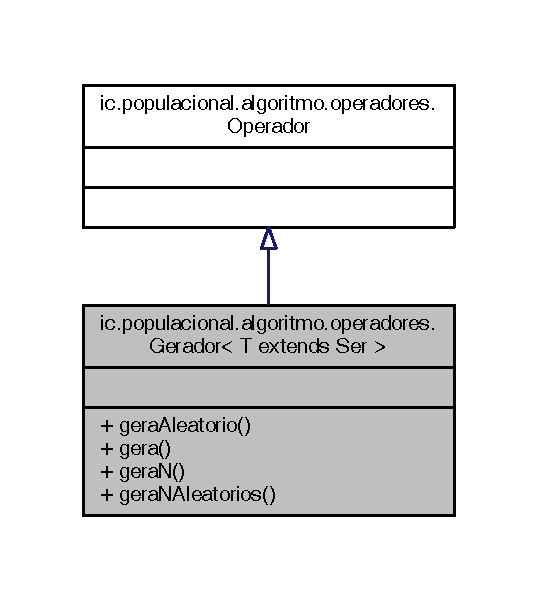
\includegraphics[width=258pt]{classic_1_1populacional_1_1algoritmo_1_1operadores_1_1_gerador_3_01_t_01extends_01_ser_01_4__inherit__graph}
\end{center}
\end{figure}


Diagrama de colaboração para ic.\-populacional.\-algoritmo.\-operadores.\-Gerador$<$ T extends Ser $>$\-:\nopagebreak
\begin{figure}[H]
\begin{center}
\leavevmode
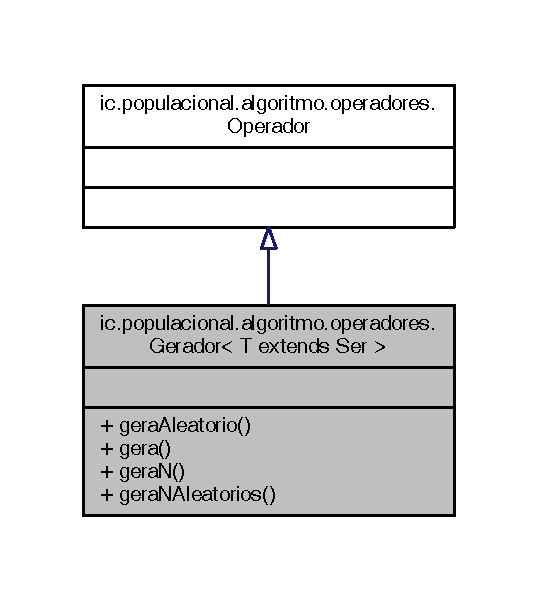
\includegraphics[width=258pt]{classic_1_1populacional_1_1algoritmo_1_1operadores_1_1_gerador_3_01_t_01extends_01_ser_01_4__coll__graph}
\end{center}
\end{figure}
\subsection*{Métodos Públicos}
\begin{DoxyCompactItemize}
\item 
abstract T \hyperlink{classic_1_1populacional_1_1algoritmo_1_1operadores_1_1_gerador_3_01_t_01extends_01_ser_01_4_af4da005d5efc0435aa204118b00afe80}{gera\-Aleatorio} ()
\begin{DoxyCompactList}\small\item\em Retorna uma nova instância. \end{DoxyCompactList}\item 
abstract T \hyperlink{classic_1_1populacional_1_1algoritmo_1_1operadores_1_1_gerador_3_01_t_01extends_01_ser_01_4_afa90423ad3e11f2795583c2bc91b163b}{gera} ()
\begin{DoxyCompactList}\small\item\em Retorna uma nova instância de ser, sem atribuição de características. \end{DoxyCompactList}\item 
Array\-List$<$ T $>$ \hyperlink{classic_1_1populacional_1_1algoritmo_1_1operadores_1_1_gerador_3_01_t_01extends_01_ser_01_4_aaec94d77b3c8b040639d2d138e0d0d86}{gera\-N} (int n)
\begin{DoxyCompactList}\small\item\em Retorna n novas instâncias. \end{DoxyCompactList}\item 
Array\-List$<$ T $>$ \hyperlink{classic_1_1populacional_1_1algoritmo_1_1operadores_1_1_gerador_3_01_t_01extends_01_ser_01_4_a3dc5afd018e47d5036123df91a542c4d}{gera\-N\-Aleatorios} (int n)
\begin{DoxyCompactList}\small\item\em Retorna n novas instâncias geradas aleatoriamente. \end{DoxyCompactList}\end{DoxyCompactItemize}


\subsection{Descrição Detalhada}
\begin{DoxyAuthor}{Autor}
Victor de Lima Soares 
\end{DoxyAuthor}


\subsection{Métodos}
\hypertarget{classic_1_1populacional_1_1algoritmo_1_1operadores_1_1_gerador_3_01_t_01extends_01_ser_01_4_afa90423ad3e11f2795583c2bc91b163b}{\index{ic\-::populacional\-::algoritmo\-::operadores\-::\-Gerador$<$ T extends Ser $>$@{ic\-::populacional\-::algoritmo\-::operadores\-::\-Gerador$<$ T extends Ser $>$}!gera@{gera}}
\index{gera@{gera}!ic::populacional::algoritmo::operadores::Gerador< T extends Ser >@{ic\-::populacional\-::algoritmo\-::operadores\-::\-Gerador$<$ T extends Ser $>$}}
\subsubsection[{gera}]{\setlength{\rightskip}{0pt plus 5cm}abstract T ic.\-populacional.\-algoritmo.\-operadores.\-Gerador$<$ T extends Ser $>$.gera (
\begin{DoxyParamCaption}
{}
\end{DoxyParamCaption}
)\hspace{0.3cm}{\ttfamily [abstract]}}}\label{classic_1_1populacional_1_1algoritmo_1_1operadores_1_1_gerador_3_01_t_01extends_01_ser_01_4_afa90423ad3e11f2795583c2bc91b163b}


Retorna uma nova instância de ser, sem atribuição de características. 

Esse método deve gerar um ser, oriundo de um processamento mais leve que \hyperlink{classic_1_1populacional_1_1algoritmo_1_1operadores_1_1_gerador_3_01_t_01extends_01_ser_01_4_af4da005d5efc0435aa204118b00afe80}{gera\-Aleatorio()}.

Enquanto \hyperlink{classic_1_1populacional_1_1algoritmo_1_1operadores_1_1_gerador_3_01_t_01extends_01_ser_01_4_af4da005d5efc0435aa204118b00afe80}{gera\-Aleatorio()} visa a criação de um ser completo, possivelmente com características aleatórias; esse método visa a geração de uma instância para manipulação, possivelmente para um atribuição mais elaborada de características; e.\-g, novo ser para receber o resultado de uma recombinação (Motivação nesse caso seria puramente por desempenho).

Essa cópia deverá ser uma nova instância. E o método não deverá receber parâmetros, pois o mesmo será usado e partes diversas da A\-P\-I, que não consideram sobrecargas.

\begin{DoxyReturn}{Retorna}
Nova instância de ser. 
\end{DoxyReturn}
\hypertarget{classic_1_1populacional_1_1algoritmo_1_1operadores_1_1_gerador_3_01_t_01extends_01_ser_01_4_af4da005d5efc0435aa204118b00afe80}{\index{ic\-::populacional\-::algoritmo\-::operadores\-::\-Gerador$<$ T extends Ser $>$@{ic\-::populacional\-::algoritmo\-::operadores\-::\-Gerador$<$ T extends Ser $>$}!gera\-Aleatorio@{gera\-Aleatorio}}
\index{gera\-Aleatorio@{gera\-Aleatorio}!ic::populacional::algoritmo::operadores::Gerador< T extends Ser >@{ic\-::populacional\-::algoritmo\-::operadores\-::\-Gerador$<$ T extends Ser $>$}}
\subsubsection[{gera\-Aleatorio}]{\setlength{\rightskip}{0pt plus 5cm}abstract T ic.\-populacional.\-algoritmo.\-operadores.\-Gerador$<$ T extends Ser $>$.gera\-Aleatorio (
\begin{DoxyParamCaption}
{}
\end{DoxyParamCaption}
)\hspace{0.3cm}{\ttfamily [abstract]}}}\label{classic_1_1populacional_1_1algoritmo_1_1operadores_1_1_gerador_3_01_t_01extends_01_ser_01_4_af4da005d5efc0435aa204118b00afe80}


Retorna uma nova instância. 

Essa cópia deverá ser uma nova instância. E o método não deverá receber parâmetros, pois o mesmo será usado e partes diversas da A\-P\-I, que não consideram sobrecargas.

\begin{DoxyReturn}{Retorna}
Nova instância de ser. 
\end{DoxyReturn}
\hypertarget{classic_1_1populacional_1_1algoritmo_1_1operadores_1_1_gerador_3_01_t_01extends_01_ser_01_4_aaec94d77b3c8b040639d2d138e0d0d86}{\index{ic\-::populacional\-::algoritmo\-::operadores\-::\-Gerador$<$ T extends Ser $>$@{ic\-::populacional\-::algoritmo\-::operadores\-::\-Gerador$<$ T extends Ser $>$}!gera\-N@{gera\-N}}
\index{gera\-N@{gera\-N}!ic::populacional::algoritmo::operadores::Gerador< T extends Ser >@{ic\-::populacional\-::algoritmo\-::operadores\-::\-Gerador$<$ T extends Ser $>$}}
\subsubsection[{gera\-N}]{\setlength{\rightskip}{0pt plus 5cm}Array\-List$<$T$>$ ic.\-populacional.\-algoritmo.\-operadores.\-Gerador$<$ T extends Ser $>$.gera\-N (
\begin{DoxyParamCaption}
\item[{int}]{n}
\end{DoxyParamCaption}
)}}\label{classic_1_1populacional_1_1algoritmo_1_1operadores_1_1_gerador_3_01_t_01extends_01_ser_01_4_aaec94d77b3c8b040639d2d138e0d0d86}


Retorna n novas instâncias. 


\begin{DoxyParams}{Parâmetros}
{\em n} & Numero de instâncias necessárias. \\
\hline
\end{DoxyParams}
\begin{DoxyReturn}{Retorna}
Uma coleção de seres recém criados.
\end{DoxyReturn}
\begin{DoxySeeAlso}{Veja também}
\hyperlink{classic_1_1populacional_1_1algoritmo_1_1operadores_1_1_gerador_3_01_t_01extends_01_ser_01_4_afa90423ad3e11f2795583c2bc91b163b}{gera()} 
\end{DoxySeeAlso}
\hypertarget{classic_1_1populacional_1_1algoritmo_1_1operadores_1_1_gerador_3_01_t_01extends_01_ser_01_4_a3dc5afd018e47d5036123df91a542c4d}{\index{ic\-::populacional\-::algoritmo\-::operadores\-::\-Gerador$<$ T extends Ser $>$@{ic\-::populacional\-::algoritmo\-::operadores\-::\-Gerador$<$ T extends Ser $>$}!gera\-N\-Aleatorios@{gera\-N\-Aleatorios}}
\index{gera\-N\-Aleatorios@{gera\-N\-Aleatorios}!ic::populacional::algoritmo::operadores::Gerador< T extends Ser >@{ic\-::populacional\-::algoritmo\-::operadores\-::\-Gerador$<$ T extends Ser $>$}}
\subsubsection[{gera\-N\-Aleatorios}]{\setlength{\rightskip}{0pt plus 5cm}Array\-List$<$T$>$ ic.\-populacional.\-algoritmo.\-operadores.\-Gerador$<$ T extends Ser $>$.gera\-N\-Aleatorios (
\begin{DoxyParamCaption}
\item[{int}]{n}
\end{DoxyParamCaption}
)}}\label{classic_1_1populacional_1_1algoritmo_1_1operadores_1_1_gerador_3_01_t_01extends_01_ser_01_4_a3dc5afd018e47d5036123df91a542c4d}


Retorna n novas instâncias geradas aleatoriamente. 


\begin{DoxyParams}{Parâmetros}
{\em n} & Numero de instâncias necessárias. \\
\hline
\end{DoxyParams}
\begin{DoxyReturn}{Retorna}
Uma coleção de seres recém criados.
\end{DoxyReturn}
\begin{DoxySeeAlso}{Veja também}
\hyperlink{classic_1_1populacional_1_1algoritmo_1_1operadores_1_1_gerador_3_01_t_01extends_01_ser_01_4_af4da005d5efc0435aa204118b00afe80}{gera\-Aleatorio()} 
\end{DoxySeeAlso}


A documentação para esta classe foi gerada a partir do seguinte arquivo\-:\begin{DoxyCompactItemize}
\item 
C\-:/\-Users/\-Victor/workplace/\-Net\-Beans\-Projects/\-Inteligencia Computacional/src/ic/populacional/algoritmo/operadores/\hyperlink{_gerador_8java}{Gerador.\-java}\end{DoxyCompactItemize}

\hypertarget{classic_1_1populacional_1_1seres_1_1permutacoes_1_1_gerador_permutacoes}{\section{Referência da Classe ic.\-populacional.\-seres.\-permutacoes.\-Gerador\-Permutacoes}
\label{classic_1_1populacional_1_1seres_1_1permutacoes_1_1_gerador_permutacoes}\index{ic.\-populacional.\-seres.\-permutacoes.\-Gerador\-Permutacoes@{ic.\-populacional.\-seres.\-permutacoes.\-Gerador\-Permutacoes}}
}


Diagrama de Hierarquia para ic.\-populacional.\-seres.\-permutacoes.\-Gerador\-Permutacoes\-:
\nopagebreak
\begin{figure}[H]
\begin{center}
\leavevmode
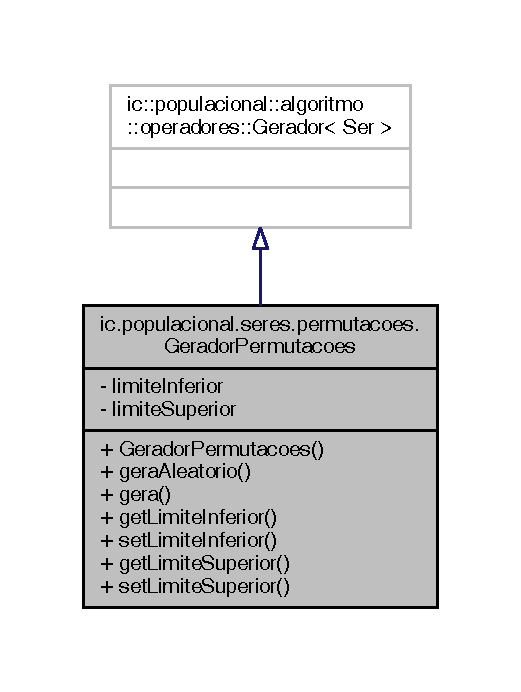
\includegraphics[width=250pt]{classic_1_1populacional_1_1seres_1_1permutacoes_1_1_gerador_permutacoes__inherit__graph}
\end{center}
\end{figure}


Diagrama de colaboração para ic.\-populacional.\-seres.\-permutacoes.\-Gerador\-Permutacoes\-:
\nopagebreak
\begin{figure}[H]
\begin{center}
\leavevmode
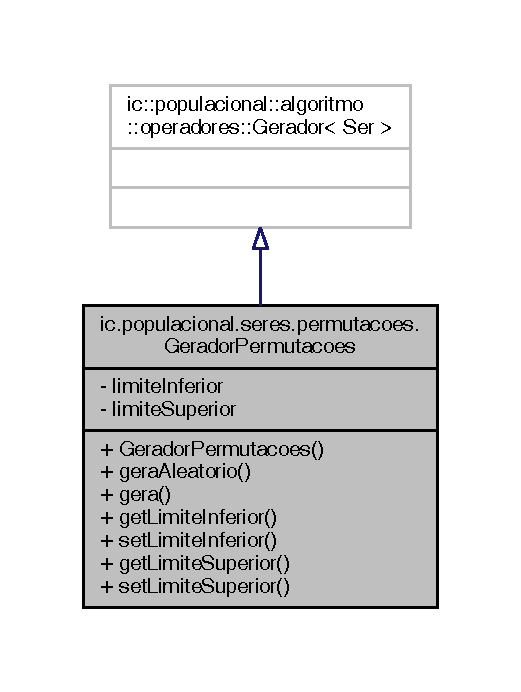
\includegraphics[width=250pt]{classic_1_1populacional_1_1seres_1_1permutacoes_1_1_gerador_permutacoes__coll__graph}
\end{center}
\end{figure}
\subsection*{Métodos Públicos}
\begin{DoxyCompactItemize}
\item 
\hyperlink{classic_1_1populacional_1_1seres_1_1permutacoes_1_1_gerador_permutacoes_a2b9aedbd540c20e9ef4abbec2a80e383}{Gerador\-Permutacoes} (int \hyperlink{classic_1_1populacional_1_1seres_1_1permutacoes_1_1_gerador_permutacoes_a1e57711cdca6ca1ae36f4ded9ca89cc8}{limite\-Inferior}, int \hyperlink{classic_1_1populacional_1_1seres_1_1permutacoes_1_1_gerador_permutacoes_af140d7298a0bb2b8fc5297474228122f}{limite\-Superior})
\item 
Ser\-Permutacao \hyperlink{classic_1_1populacional_1_1seres_1_1permutacoes_1_1_gerador_permutacoes_ab44a312d6089675ab1a89bb7619739aa}{gera\-Aleatorio} ()
\item 
Ser\-Permutacao \hyperlink{classic_1_1populacional_1_1seres_1_1permutacoes_1_1_gerador_permutacoes_a49bc0197f542704a818284c2d286e6d9}{gera} ()
\item 
int \hyperlink{classic_1_1populacional_1_1seres_1_1permutacoes_1_1_gerador_permutacoes_a1ab108c463da60f9925bed5367b03de4}{get\-Limite\-Inferior} ()
\item 
void \hyperlink{classic_1_1populacional_1_1seres_1_1permutacoes_1_1_gerador_permutacoes_aa5b4716c1212fb1fb5e48536a618407f}{set\-Limite\-Inferior} (int \hyperlink{classic_1_1populacional_1_1seres_1_1permutacoes_1_1_gerador_permutacoes_a1e57711cdca6ca1ae36f4ded9ca89cc8}{limite\-Inferior})
\item 
int \hyperlink{classic_1_1populacional_1_1seres_1_1permutacoes_1_1_gerador_permutacoes_a0fdb3341ed4cfee7449d1d0287715a78}{get\-Limite\-Superior} ()
\item 
void \hyperlink{classic_1_1populacional_1_1seres_1_1permutacoes_1_1_gerador_permutacoes_aa6fe8cf54287162db359df8d12818ae5}{set\-Limite\-Superior} (int \hyperlink{classic_1_1populacional_1_1seres_1_1permutacoes_1_1_gerador_permutacoes_af140d7298a0bb2b8fc5297474228122f}{limite\-Superior})
\end{DoxyCompactItemize}
\subsection*{Atributos Privados}
\begin{DoxyCompactItemize}
\item 
int \hyperlink{classic_1_1populacional_1_1seres_1_1permutacoes_1_1_gerador_permutacoes_a1e57711cdca6ca1ae36f4ded9ca89cc8}{limite\-Inferior}
\item 
int \hyperlink{classic_1_1populacional_1_1seres_1_1permutacoes_1_1_gerador_permutacoes_af140d7298a0bb2b8fc5297474228122f}{limite\-Superior}
\end{DoxyCompactItemize}


\subsection{Descrição Detalhada}
\begin{DoxyAuthor}{Autor}
Victor de Lima Soares 
\end{DoxyAuthor}


\subsection{Construtores \& Destrutores}
\hypertarget{classic_1_1populacional_1_1seres_1_1permutacoes_1_1_gerador_permutacoes_a2b9aedbd540c20e9ef4abbec2a80e383}{\index{ic\-::populacional\-::seres\-::permutacoes\-::\-Gerador\-Permutacoes@{ic\-::populacional\-::seres\-::permutacoes\-::\-Gerador\-Permutacoes}!Gerador\-Permutacoes@{Gerador\-Permutacoes}}
\index{Gerador\-Permutacoes@{Gerador\-Permutacoes}!ic::populacional::seres::permutacoes::GeradorPermutacoes@{ic\-::populacional\-::seres\-::permutacoes\-::\-Gerador\-Permutacoes}}
\subsubsection[{Gerador\-Permutacoes}]{\setlength{\rightskip}{0pt plus 5cm}ic.\-populacional.\-seres.\-permutacoes.\-Gerador\-Permutacoes.\-Gerador\-Permutacoes (
\begin{DoxyParamCaption}
\item[{int}]{limite\-Inferior, }
\item[{int}]{limite\-Superior}
\end{DoxyParamCaption}
)}}\label{classic_1_1populacional_1_1seres_1_1permutacoes_1_1_gerador_permutacoes_a2b9aedbd540c20e9ef4abbec2a80e383}


\subsection{Métodos}
\hypertarget{classic_1_1populacional_1_1seres_1_1permutacoes_1_1_gerador_permutacoes_a49bc0197f542704a818284c2d286e6d9}{\index{ic\-::populacional\-::seres\-::permutacoes\-::\-Gerador\-Permutacoes@{ic\-::populacional\-::seres\-::permutacoes\-::\-Gerador\-Permutacoes}!gera@{gera}}
\index{gera@{gera}!ic::populacional::seres::permutacoes::GeradorPermutacoes@{ic\-::populacional\-::seres\-::permutacoes\-::\-Gerador\-Permutacoes}}
\subsubsection[{gera}]{\setlength{\rightskip}{0pt plus 5cm}Ser\-Permutacao ic.\-populacional.\-seres.\-permutacoes.\-Gerador\-Permutacoes.\-gera (
\begin{DoxyParamCaption}
{}
\end{DoxyParamCaption}
)}}\label{classic_1_1populacional_1_1seres_1_1permutacoes_1_1_gerador_permutacoes_a49bc0197f542704a818284c2d286e6d9}
\hypertarget{classic_1_1populacional_1_1seres_1_1permutacoes_1_1_gerador_permutacoes_ab44a312d6089675ab1a89bb7619739aa}{\index{ic\-::populacional\-::seres\-::permutacoes\-::\-Gerador\-Permutacoes@{ic\-::populacional\-::seres\-::permutacoes\-::\-Gerador\-Permutacoes}!gera\-Aleatorio@{gera\-Aleatorio}}
\index{gera\-Aleatorio@{gera\-Aleatorio}!ic::populacional::seres::permutacoes::GeradorPermutacoes@{ic\-::populacional\-::seres\-::permutacoes\-::\-Gerador\-Permutacoes}}
\subsubsection[{gera\-Aleatorio}]{\setlength{\rightskip}{0pt plus 5cm}Ser\-Permutacao ic.\-populacional.\-seres.\-permutacoes.\-Gerador\-Permutacoes.\-gera\-Aleatorio (
\begin{DoxyParamCaption}
{}
\end{DoxyParamCaption}
)}}\label{classic_1_1populacional_1_1seres_1_1permutacoes_1_1_gerador_permutacoes_ab44a312d6089675ab1a89bb7619739aa}


Este é o diagrama das funções utilizadas por esta função\-:
\nopagebreak
\begin{figure}[H]
\begin{center}
\leavevmode
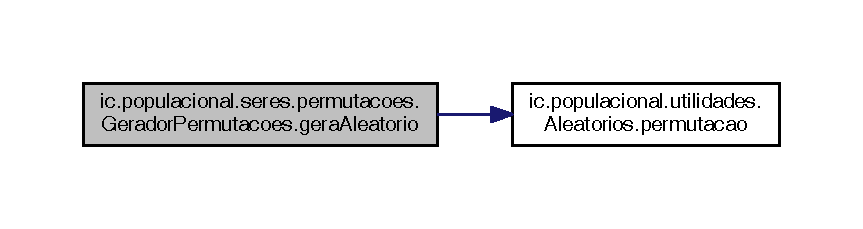
\includegraphics[width=350pt]{classic_1_1populacional_1_1seres_1_1permutacoes_1_1_gerador_permutacoes_ab44a312d6089675ab1a89bb7619739aa_cgraph}
\end{center}
\end{figure}


\hypertarget{classic_1_1populacional_1_1seres_1_1permutacoes_1_1_gerador_permutacoes_a1ab108c463da60f9925bed5367b03de4}{\index{ic\-::populacional\-::seres\-::permutacoes\-::\-Gerador\-Permutacoes@{ic\-::populacional\-::seres\-::permutacoes\-::\-Gerador\-Permutacoes}!get\-Limite\-Inferior@{get\-Limite\-Inferior}}
\index{get\-Limite\-Inferior@{get\-Limite\-Inferior}!ic::populacional::seres::permutacoes::GeradorPermutacoes@{ic\-::populacional\-::seres\-::permutacoes\-::\-Gerador\-Permutacoes}}
\subsubsection[{get\-Limite\-Inferior}]{\setlength{\rightskip}{0pt plus 5cm}int ic.\-populacional.\-seres.\-permutacoes.\-Gerador\-Permutacoes.\-get\-Limite\-Inferior (
\begin{DoxyParamCaption}
{}
\end{DoxyParamCaption}
)}}\label{classic_1_1populacional_1_1seres_1_1permutacoes_1_1_gerador_permutacoes_a1ab108c463da60f9925bed5367b03de4}
\hypertarget{classic_1_1populacional_1_1seres_1_1permutacoes_1_1_gerador_permutacoes_a0fdb3341ed4cfee7449d1d0287715a78}{\index{ic\-::populacional\-::seres\-::permutacoes\-::\-Gerador\-Permutacoes@{ic\-::populacional\-::seres\-::permutacoes\-::\-Gerador\-Permutacoes}!get\-Limite\-Superior@{get\-Limite\-Superior}}
\index{get\-Limite\-Superior@{get\-Limite\-Superior}!ic::populacional::seres::permutacoes::GeradorPermutacoes@{ic\-::populacional\-::seres\-::permutacoes\-::\-Gerador\-Permutacoes}}
\subsubsection[{get\-Limite\-Superior}]{\setlength{\rightskip}{0pt plus 5cm}int ic.\-populacional.\-seres.\-permutacoes.\-Gerador\-Permutacoes.\-get\-Limite\-Superior (
\begin{DoxyParamCaption}
{}
\end{DoxyParamCaption}
)}}\label{classic_1_1populacional_1_1seres_1_1permutacoes_1_1_gerador_permutacoes_a0fdb3341ed4cfee7449d1d0287715a78}
\hypertarget{classic_1_1populacional_1_1seres_1_1permutacoes_1_1_gerador_permutacoes_aa5b4716c1212fb1fb5e48536a618407f}{\index{ic\-::populacional\-::seres\-::permutacoes\-::\-Gerador\-Permutacoes@{ic\-::populacional\-::seres\-::permutacoes\-::\-Gerador\-Permutacoes}!set\-Limite\-Inferior@{set\-Limite\-Inferior}}
\index{set\-Limite\-Inferior@{set\-Limite\-Inferior}!ic::populacional::seres::permutacoes::GeradorPermutacoes@{ic\-::populacional\-::seres\-::permutacoes\-::\-Gerador\-Permutacoes}}
\subsubsection[{set\-Limite\-Inferior}]{\setlength{\rightskip}{0pt plus 5cm}void ic.\-populacional.\-seres.\-permutacoes.\-Gerador\-Permutacoes.\-set\-Limite\-Inferior (
\begin{DoxyParamCaption}
\item[{int}]{limite\-Inferior}
\end{DoxyParamCaption}
)}}\label{classic_1_1populacional_1_1seres_1_1permutacoes_1_1_gerador_permutacoes_aa5b4716c1212fb1fb5e48536a618407f}
\hypertarget{classic_1_1populacional_1_1seres_1_1permutacoes_1_1_gerador_permutacoes_aa6fe8cf54287162db359df8d12818ae5}{\index{ic\-::populacional\-::seres\-::permutacoes\-::\-Gerador\-Permutacoes@{ic\-::populacional\-::seres\-::permutacoes\-::\-Gerador\-Permutacoes}!set\-Limite\-Superior@{set\-Limite\-Superior}}
\index{set\-Limite\-Superior@{set\-Limite\-Superior}!ic::populacional::seres::permutacoes::GeradorPermutacoes@{ic\-::populacional\-::seres\-::permutacoes\-::\-Gerador\-Permutacoes}}
\subsubsection[{set\-Limite\-Superior}]{\setlength{\rightskip}{0pt plus 5cm}void ic.\-populacional.\-seres.\-permutacoes.\-Gerador\-Permutacoes.\-set\-Limite\-Superior (
\begin{DoxyParamCaption}
\item[{int}]{limite\-Superior}
\end{DoxyParamCaption}
)}}\label{classic_1_1populacional_1_1seres_1_1permutacoes_1_1_gerador_permutacoes_aa6fe8cf54287162db359df8d12818ae5}


\subsection{Atributos}
\hypertarget{classic_1_1populacional_1_1seres_1_1permutacoes_1_1_gerador_permutacoes_a1e57711cdca6ca1ae36f4ded9ca89cc8}{\index{ic\-::populacional\-::seres\-::permutacoes\-::\-Gerador\-Permutacoes@{ic\-::populacional\-::seres\-::permutacoes\-::\-Gerador\-Permutacoes}!limite\-Inferior@{limite\-Inferior}}
\index{limite\-Inferior@{limite\-Inferior}!ic::populacional::seres::permutacoes::GeradorPermutacoes@{ic\-::populacional\-::seres\-::permutacoes\-::\-Gerador\-Permutacoes}}
\subsubsection[{limite\-Inferior}]{\setlength{\rightskip}{0pt plus 5cm}int ic.\-populacional.\-seres.\-permutacoes.\-Gerador\-Permutacoes.\-limite\-Inferior\hspace{0.3cm}{\ttfamily [private]}}}\label{classic_1_1populacional_1_1seres_1_1permutacoes_1_1_gerador_permutacoes_a1e57711cdca6ca1ae36f4ded9ca89cc8}
\hypertarget{classic_1_1populacional_1_1seres_1_1permutacoes_1_1_gerador_permutacoes_af140d7298a0bb2b8fc5297474228122f}{\index{ic\-::populacional\-::seres\-::permutacoes\-::\-Gerador\-Permutacoes@{ic\-::populacional\-::seres\-::permutacoes\-::\-Gerador\-Permutacoes}!limite\-Superior@{limite\-Superior}}
\index{limite\-Superior@{limite\-Superior}!ic::populacional::seres::permutacoes::GeradorPermutacoes@{ic\-::populacional\-::seres\-::permutacoes\-::\-Gerador\-Permutacoes}}
\subsubsection[{limite\-Superior}]{\setlength{\rightskip}{0pt plus 5cm}int ic.\-populacional.\-seres.\-permutacoes.\-Gerador\-Permutacoes.\-limite\-Superior\hspace{0.3cm}{\ttfamily [private]}}}\label{classic_1_1populacional_1_1seres_1_1permutacoes_1_1_gerador_permutacoes_af140d7298a0bb2b8fc5297474228122f}


A documentação para esta classe foi gerada a partir do seguinte arquivo\-:\begin{DoxyCompactItemize}
\item 
C\-:/\-Users/\-Victor/workplace/\-Net\-Beans\-Projects/\-Inteligencia Computacional/src/ic/populacional/seres/permutacoes/\hyperlink{_gerador_permutacoes_8java}{Gerador\-Permutacoes.\-java}\end{DoxyCompactItemize}

\hypertarget{classic_1_1populacional_1_1utilidades_1_1_indice_aleatorio}{\section{Referência da Classe ic.\-populacional.\-utilidades.\-Indice\-Aleatorio}
\label{classic_1_1populacional_1_1utilidades_1_1_indice_aleatorio}\index{ic.\-populacional.\-utilidades.\-Indice\-Aleatorio@{ic.\-populacional.\-utilidades.\-Indice\-Aleatorio}}
}


Classe auxiliar para a recuperação de índices em listas de características ou em seres.  




Diagrama de colaboração para ic.\-populacional.\-utilidades.\-Indice\-Aleatorio\-:\nopagebreak
\begin{figure}[H]
\begin{center}
\leavevmode
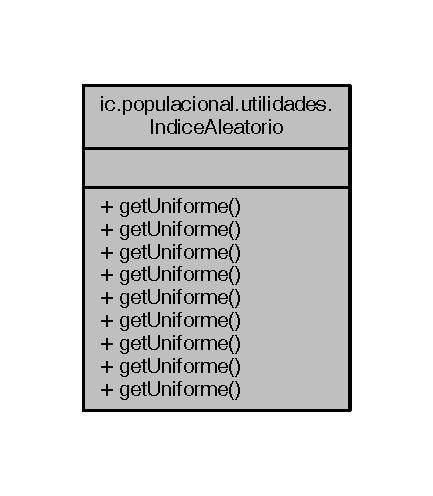
\includegraphics[width=208pt]{classic_1_1populacional_1_1utilidades_1_1_indice_aleatorio__coll__graph}
\end{center}
\end{figure}
\subsection*{Métodos Públicos Estáticos}
\begin{DoxyCompactItemize}
\item 
static final int \hyperlink{classic_1_1populacional_1_1utilidades_1_1_indice_aleatorio_ae36a71951fb007c177503efe61cd69cf}{get\-Uniforme} (Ser origem)
\begin{DoxyCompactList}\small\item\em Retorna um índice aleatório para uma característica de um ser. \end{DoxyCompactList}\item 
static final int \hyperlink{classic_1_1populacional_1_1utilidades_1_1_indice_aleatorio_aeb5e4cf0ec35489dc02c6d84a3d04744}{get\-Uniforme} (List$<$ Caracteristica $>$ origem)
\begin{DoxyCompactList}\small\item\em Retorna um índice aleatório para uma característica de um ser. \end{DoxyCompactList}\item 
static final int \hyperlink{classic_1_1populacional_1_1utilidades_1_1_indice_aleatorio_adfc01422d107da549e4925692d2a5514}{get\-Uniforme} (Ser origem, int limite\-Inferior, int limite\-Superior)
\begin{DoxyCompactList}\small\item\em Retorna um índice aleatório para uma característica de um ser. \end{DoxyCompactList}\item 
static final int \hyperlink{classic_1_1populacional_1_1utilidades_1_1_indice_aleatorio_ab63b5d88c777b08a27d9bf3510360132}{get\-Uniforme} (List$<$ Caracteristica $>$ origem, int limite\-Inferior, int limite\-Superior)
\begin{DoxyCompactList}\small\item\em Retorna um índice aleatório para uma característica de um ser. \end{DoxyCompactList}\item 
static final List$<$ Integer $>$ \hyperlink{classic_1_1populacional_1_1utilidades_1_1_indice_aleatorio_ad173cfec1a8b8386148439711460bd06}{get\-Uniforme} (Ser origem, int n\-Numeros)
\begin{DoxyCompactList}\small\item\em Retorna n índices aleatórios para características de um ser. \end{DoxyCompactList}\item 
static final List$<$ Integer $>$ \hyperlink{classic_1_1populacional_1_1utilidades_1_1_indice_aleatorio_acd15ec50342b37c7359b952924a092f2}{get\-Uniforme} (List$<$ Caracteristica $>$ origem, int n\-Numeros)
\begin{DoxyCompactList}\small\item\em Retorna {\itshape n} índices aleatórios para características de um ser. \end{DoxyCompactList}\item 
static final List$<$ Integer $>$ \hyperlink{classic_1_1populacional_1_1utilidades_1_1_indice_aleatorio_a6dc51d0095217dbfaf7b0140407d36c6}{get\-Uniforme} (Ser origem, int n\-Numeros, int limite\-Inferior, int limite\-Superior)
\begin{DoxyCompactList}\small\item\em Retorna {\itshape n} índices aleatórios para características de um ser. \end{DoxyCompactList}\item 
static final List$<$ Integer $>$ \hyperlink{classic_1_1populacional_1_1utilidades_1_1_indice_aleatorio_aef72ba4471671f92147e0904ce1e599f}{get\-Uniforme} (List$<$ Caracteristica $>$ origem, int n\-Numeros, int limite\-Inferior, int limite\-Superior)
\begin{DoxyCompactList}\small\item\em Retorna {\itshape n} índices aleatórios para características de um ser. \end{DoxyCompactList}\item 
static final Array\-List$<$ Integer $>$ \hyperlink{classic_1_1populacional_1_1utilidades_1_1_indice_aleatorio_a453201b8ee1e4468d3ebe80f0b5188cb}{get\-Uniforme} (Populacao origem, int n\-Numeros)
\begin{DoxyCompactList}\small\item\em Retorna n índices aleatórios para seres em uma população. \end{DoxyCompactList}\end{DoxyCompactItemize}


\subsection{Descrição Detalhada}
Classe auxiliar para a recuperação de índices em listas de características ou em seres. 

\begin{DoxyVersion}{Versão}
1.\-0 
\end{DoxyVersion}
\begin{DoxyAuthor}{Autor}
Victor de Lima Soares 
\end{DoxyAuthor}


\subsection{Métodos}
\hypertarget{classic_1_1populacional_1_1utilidades_1_1_indice_aleatorio_ae36a71951fb007c177503efe61cd69cf}{\index{ic\-::populacional\-::utilidades\-::\-Indice\-Aleatorio@{ic\-::populacional\-::utilidades\-::\-Indice\-Aleatorio}!get\-Uniforme@{get\-Uniforme}}
\index{get\-Uniforme@{get\-Uniforme}!ic::populacional::utilidades::IndiceAleatorio@{ic\-::populacional\-::utilidades\-::\-Indice\-Aleatorio}}
\subsubsection[{get\-Uniforme}]{\setlength{\rightskip}{0pt plus 5cm}static final int ic.\-populacional.\-utilidades.\-Indice\-Aleatorio.\-get\-Uniforme (
\begin{DoxyParamCaption}
\item[{Ser}]{origem}
\end{DoxyParamCaption}
)\hspace{0.3cm}{\ttfamily [static]}}}\label{classic_1_1populacional_1_1utilidades_1_1_indice_aleatorio_ae36a71951fb007c177503efe61cd69cf}


Retorna um índice aleatório para uma característica de um ser. 

Distribuição uniforme. 

Gerador seguro para múltiplas Threads. 

\begin{DoxySince}{Desde}
1.\-0 
\end{DoxySince}

\begin{DoxyParams}{Parâmetros}
{\em origem} & Ser cujo índice da característica é desejado. \\
\hline
\end{DoxyParams}
\begin{DoxyReturn}{Retorna}
Índice escolhido aleatoriamente. 
\end{DoxyReturn}


Este é o diagrama das funções que utilizam esta função\-:\nopagebreak
\begin{figure}[H]
\begin{center}
\leavevmode
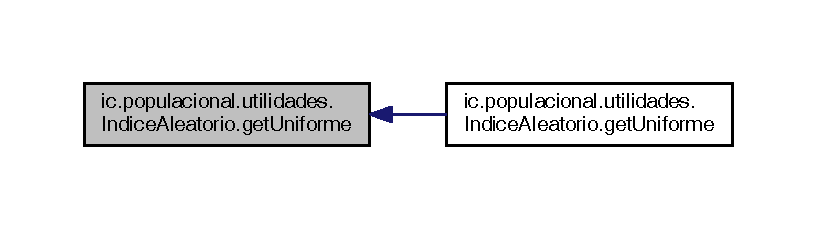
\includegraphics[width=350pt]{classic_1_1populacional_1_1utilidades_1_1_indice_aleatorio_ae36a71951fb007c177503efe61cd69cf_icgraph}
\end{center}
\end{figure}


\hypertarget{classic_1_1populacional_1_1utilidades_1_1_indice_aleatorio_aeb5e4cf0ec35489dc02c6d84a3d04744}{\index{ic\-::populacional\-::utilidades\-::\-Indice\-Aleatorio@{ic\-::populacional\-::utilidades\-::\-Indice\-Aleatorio}!get\-Uniforme@{get\-Uniforme}}
\index{get\-Uniforme@{get\-Uniforme}!ic::populacional::utilidades::IndiceAleatorio@{ic\-::populacional\-::utilidades\-::\-Indice\-Aleatorio}}
\subsubsection[{get\-Uniforme}]{\setlength{\rightskip}{0pt plus 5cm}static final int ic.\-populacional.\-utilidades.\-Indice\-Aleatorio.\-get\-Uniforme (
\begin{DoxyParamCaption}
\item[{List$<$ Caracteristica $>$}]{origem}
\end{DoxyParamCaption}
)\hspace{0.3cm}{\ttfamily [static]}}}\label{classic_1_1populacional_1_1utilidades_1_1_indice_aleatorio_aeb5e4cf0ec35489dc02c6d84a3d04744}


Retorna um índice aleatório para uma característica de um ser. 

Distribuição uniforme. 

Gerador seguro para múltiplas Threads. 

\begin{DoxySince}{Desde}
1.\-0 
\end{DoxySince}

\begin{DoxyParams}{Parâmetros}
{\em origem} & Lista de características cujo índice de uma delas é desejado. \\
\hline
\end{DoxyParams}
\begin{DoxyReturn}{Retorna}
Índice escolhido aleatoriamente. 
\end{DoxyReturn}
\hypertarget{classic_1_1populacional_1_1utilidades_1_1_indice_aleatorio_adfc01422d107da549e4925692d2a5514}{\index{ic\-::populacional\-::utilidades\-::\-Indice\-Aleatorio@{ic\-::populacional\-::utilidades\-::\-Indice\-Aleatorio}!get\-Uniforme@{get\-Uniforme}}
\index{get\-Uniforme@{get\-Uniforme}!ic::populacional::utilidades::IndiceAleatorio@{ic\-::populacional\-::utilidades\-::\-Indice\-Aleatorio}}
\subsubsection[{get\-Uniforme}]{\setlength{\rightskip}{0pt plus 5cm}static final int ic.\-populacional.\-utilidades.\-Indice\-Aleatorio.\-get\-Uniforme (
\begin{DoxyParamCaption}
\item[{Ser}]{origem, }
\item[{int}]{limite\-Inferior, }
\item[{int}]{limite\-Superior}
\end{DoxyParamCaption}
)\hspace{0.3cm}{\ttfamily [static]}}}\label{classic_1_1populacional_1_1utilidades_1_1_indice_aleatorio_adfc01422d107da549e4925692d2a5514}


Retorna um índice aleatório para uma característica de um ser. 

Distribuição uniforme. 

Gerador seguro para múltiplas Threads. 

\begin{DoxySince}{Desde}
1.\-0 
\end{DoxySince}

\begin{DoxyParams}{Parâmetros}
{\em origem} & Ser cujo índice de uma característica é desejado. \\
\hline
{\em limite\-Inferior} & Limite inferior(índice), maior que zero. \\
\hline
{\em limite\-Superior} & Limite superior(índice), maior que zero. \\
\hline
\end{DoxyParams}
\begin{DoxyReturn}{Retorna}
Índice escolhido aleatoriamente.
\end{DoxyReturn}

\begin{DoxyExceptions}{Exceções}
{\em Illegal\-Argument\-Exception} & Se 
\begin{DoxyItemize}
\item Limite inferior for menor que zero;  
\item Limite superior for menor que o limite inferior;  
\item Limite superior for maior {\bfseries ou igual} ao tamanho do ser, ou lista de características;  
\end{DoxyItemize}\\
\hline
\end{DoxyExceptions}


Este é o diagrama das funções utilizadas por esta função\-:\nopagebreak
\begin{figure}[H]
\begin{center}
\leavevmode
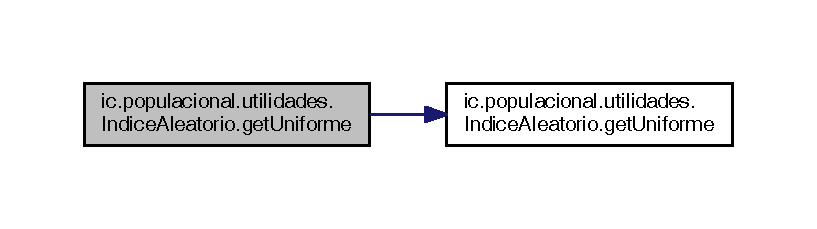
\includegraphics[width=350pt]{classic_1_1populacional_1_1utilidades_1_1_indice_aleatorio_adfc01422d107da549e4925692d2a5514_cgraph}
\end{center}
\end{figure}


\hypertarget{classic_1_1populacional_1_1utilidades_1_1_indice_aleatorio_ab63b5d88c777b08a27d9bf3510360132}{\index{ic\-::populacional\-::utilidades\-::\-Indice\-Aleatorio@{ic\-::populacional\-::utilidades\-::\-Indice\-Aleatorio}!get\-Uniforme@{get\-Uniforme}}
\index{get\-Uniforme@{get\-Uniforme}!ic::populacional::utilidades::IndiceAleatorio@{ic\-::populacional\-::utilidades\-::\-Indice\-Aleatorio}}
\subsubsection[{get\-Uniforme}]{\setlength{\rightskip}{0pt plus 5cm}static final int ic.\-populacional.\-utilidades.\-Indice\-Aleatorio.\-get\-Uniforme (
\begin{DoxyParamCaption}
\item[{List$<$ Caracteristica $>$}]{origem, }
\item[{int}]{limite\-Inferior, }
\item[{int}]{limite\-Superior}
\end{DoxyParamCaption}
)\hspace{0.3cm}{\ttfamily [static]}}}\label{classic_1_1populacional_1_1utilidades_1_1_indice_aleatorio_ab63b5d88c777b08a27d9bf3510360132}


Retorna um índice aleatório para uma característica de um ser. 

Distribuição uniforme. 

Gerador seguro para múltiplas Threads. 

\begin{DoxySince}{Desde}
1.\-0 
\end{DoxySince}

\begin{DoxyParams}{Parâmetros}
{\em origem} & Lista de características cujo índice de uma delas é desejado. \\
\hline
{\em limite\-Inferior} & Limite inferior(índice), maior que zero. \\
\hline
{\em limite\-Superior} & Limite superior(índice,inclusive), maior que zero. \\
\hline
\end{DoxyParams}
\begin{DoxyReturn}{Retorna}
Índice escolhido aleatoriamente.
\end{DoxyReturn}

\begin{DoxyExceptions}{Exceções}
{\em Illegal\-Argument\-Exception} & Se 
\begin{DoxyItemize}
\item Limite inferior for menor que zero;  
\item Limite superior for menor que o limite inferior;  
\item Limite superior for maior {\bfseries ou igual} ao tamanho do ser, ou lista de características;  
\end{DoxyItemize}\\
\hline
\end{DoxyExceptions}
\hypertarget{classic_1_1populacional_1_1utilidades_1_1_indice_aleatorio_ad173cfec1a8b8386148439711460bd06}{\index{ic\-::populacional\-::utilidades\-::\-Indice\-Aleatorio@{ic\-::populacional\-::utilidades\-::\-Indice\-Aleatorio}!get\-Uniforme@{get\-Uniforme}}
\index{get\-Uniforme@{get\-Uniforme}!ic::populacional::utilidades::IndiceAleatorio@{ic\-::populacional\-::utilidades\-::\-Indice\-Aleatorio}}
\subsubsection[{get\-Uniforme}]{\setlength{\rightskip}{0pt plus 5cm}static final List$<$Integer$>$ ic.\-populacional.\-utilidades.\-Indice\-Aleatorio.\-get\-Uniforme (
\begin{DoxyParamCaption}
\item[{Ser}]{origem, }
\item[{int}]{n\-Numeros}
\end{DoxyParamCaption}
)\hspace{0.3cm}{\ttfamily [static]}}}\label{classic_1_1populacional_1_1utilidades_1_1_indice_aleatorio_ad173cfec1a8b8386148439711460bd06}


Retorna n índices aleatórios para características de um ser. 

Distribuição uniforme. 

Gerador seguro para múltiplas Threads. 

\begin{DoxySince}{Desde}
1.\-0 
\end{DoxySince}

\begin{DoxyParams}{Parâmetros}
{\em origem} & Ser cujos índices de características são desejados. \\
\hline
{\em n\-Numeros} & Número de índices desejados. \\
\hline
\end{DoxyParams}
\begin{DoxyReturn}{Retorna}
Índices escolhidos aleatoriamente, sem repetição. 
\end{DoxyReturn}


Este é o diagrama das funções utilizadas por esta função\-:\nopagebreak
\begin{figure}[H]
\begin{center}
\leavevmode
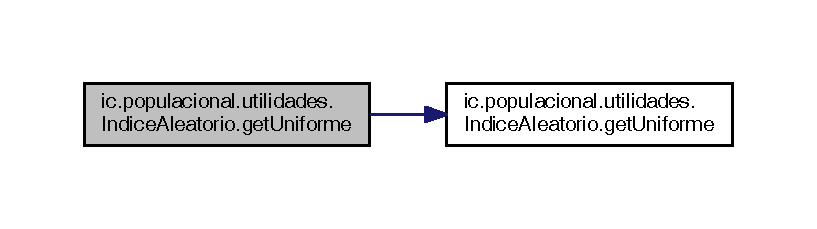
\includegraphics[width=350pt]{classic_1_1populacional_1_1utilidades_1_1_indice_aleatorio_ad173cfec1a8b8386148439711460bd06_cgraph}
\end{center}
\end{figure}


\hypertarget{classic_1_1populacional_1_1utilidades_1_1_indice_aleatorio_acd15ec50342b37c7359b952924a092f2}{\index{ic\-::populacional\-::utilidades\-::\-Indice\-Aleatorio@{ic\-::populacional\-::utilidades\-::\-Indice\-Aleatorio}!get\-Uniforme@{get\-Uniforme}}
\index{get\-Uniforme@{get\-Uniforme}!ic::populacional::utilidades::IndiceAleatorio@{ic\-::populacional\-::utilidades\-::\-Indice\-Aleatorio}}
\subsubsection[{get\-Uniforme}]{\setlength{\rightskip}{0pt plus 5cm}static final List$<$Integer$>$ ic.\-populacional.\-utilidades.\-Indice\-Aleatorio.\-get\-Uniforme (
\begin{DoxyParamCaption}
\item[{List$<$ Caracteristica $>$}]{origem, }
\item[{int}]{n\-Numeros}
\end{DoxyParamCaption}
)\hspace{0.3cm}{\ttfamily [static]}}}\label{classic_1_1populacional_1_1utilidades_1_1_indice_aleatorio_acd15ec50342b37c7359b952924a092f2}


Retorna {\itshape n} índices aleatórios para características de um ser. 

Distribuição uniforme. 

Gerador seguro para múltiplas Threads. 

\begin{DoxySince}{Desde}
1.\-0 
\end{DoxySince}

\begin{DoxyParams}{Parâmetros}
{\em origem} & Lista de características de origem\-: define os limites para a geração. \\
\hline
{\em n\-Numeros} & Número de índices desejados. \\
\hline
\end{DoxyParams}
\begin{DoxyReturn}{Retorna}
Índices escolhidos aleatoriamente, {\bfseries sem repetição}.
\end{DoxyReturn}

\begin{DoxyExceptions}{Exceções}
{\em Illegal\-Argument\-Exception} & Se 
\begin{DoxyItemize}
\item O número de índices pedidos for maior que o tamanho do ser.  
\end{DoxyItemize}\\
\hline
\end{DoxyExceptions}
\hypertarget{classic_1_1populacional_1_1utilidades_1_1_indice_aleatorio_a6dc51d0095217dbfaf7b0140407d36c6}{\index{ic\-::populacional\-::utilidades\-::\-Indice\-Aleatorio@{ic\-::populacional\-::utilidades\-::\-Indice\-Aleatorio}!get\-Uniforme@{get\-Uniforme}}
\index{get\-Uniforme@{get\-Uniforme}!ic::populacional::utilidades::IndiceAleatorio@{ic\-::populacional\-::utilidades\-::\-Indice\-Aleatorio}}
\subsubsection[{get\-Uniforme}]{\setlength{\rightskip}{0pt plus 5cm}static final List$<$Integer$>$ ic.\-populacional.\-utilidades.\-Indice\-Aleatorio.\-get\-Uniforme (
\begin{DoxyParamCaption}
\item[{Ser}]{origem, }
\item[{int}]{n\-Numeros, }
\item[{int}]{limite\-Inferior, }
\item[{int}]{limite\-Superior}
\end{DoxyParamCaption}
)\hspace{0.3cm}{\ttfamily [static]}}}\label{classic_1_1populacional_1_1utilidades_1_1_indice_aleatorio_a6dc51d0095217dbfaf7b0140407d36c6}


Retorna {\itshape n} índices aleatórios para características de um ser. 

Distribuição uniforme. 

Gerador seguro para múltiplas Threads. 

\begin{DoxySince}{Desde}
1.\-0 
\end{DoxySince}

\begin{DoxyParams}{Parâmetros}
{\em origem} & Ser de origem\-: define os limites para a geração. \\
\hline
{\em n\-Numeros} & Número de índices desejados. \\
\hline
{\em limite\-Inferior} & Limite inferior(índice), maior que zero. \\
\hline
{\em limite\-Superior} & Limite superior(índice), maior que zero. \\
\hline
\end{DoxyParams}
\begin{DoxyReturn}{Retorna}
Índices escolhidos aleatoriamente, {\bfseries sem repetição}.
\end{DoxyReturn}

\begin{DoxyExceptions}{Exceções}
{\em Illegal\-Argument\-Exception} & Se 
\begin{DoxyItemize}
\item O número de índices pedidos for maior que o tamanho do ser.  
\item Limite inferior for menor que zero;  
\item Limite superior for menor que o limite inferior;  
\item Limite superior for maior {\bfseries ou igual} ao tamanho do ser, ou lista de características;  
\item Número de índices for maior que o tamanho do intervalo entre os limites.  
\end{DoxyItemize}\\
\hline
\end{DoxyExceptions}


Este é o diagrama das funções utilizadas por esta função\-:\nopagebreak
\begin{figure}[H]
\begin{center}
\leavevmode
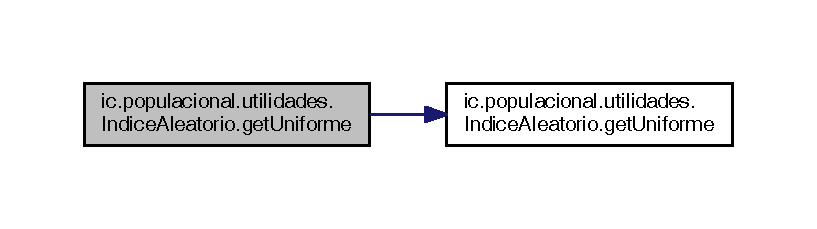
\includegraphics[width=350pt]{classic_1_1populacional_1_1utilidades_1_1_indice_aleatorio_a6dc51d0095217dbfaf7b0140407d36c6_cgraph}
\end{center}
\end{figure}


\hypertarget{classic_1_1populacional_1_1utilidades_1_1_indice_aleatorio_aef72ba4471671f92147e0904ce1e599f}{\index{ic\-::populacional\-::utilidades\-::\-Indice\-Aleatorio@{ic\-::populacional\-::utilidades\-::\-Indice\-Aleatorio}!get\-Uniforme@{get\-Uniforme}}
\index{get\-Uniforme@{get\-Uniforme}!ic::populacional::utilidades::IndiceAleatorio@{ic\-::populacional\-::utilidades\-::\-Indice\-Aleatorio}}
\subsubsection[{get\-Uniforme}]{\setlength{\rightskip}{0pt plus 5cm}static final List$<$Integer$>$ ic.\-populacional.\-utilidades.\-Indice\-Aleatorio.\-get\-Uniforme (
\begin{DoxyParamCaption}
\item[{List$<$ Caracteristica $>$}]{origem, }
\item[{int}]{n\-Numeros, }
\item[{int}]{limite\-Inferior, }
\item[{int}]{limite\-Superior}
\end{DoxyParamCaption}
)\hspace{0.3cm}{\ttfamily [static]}}}\label{classic_1_1populacional_1_1utilidades_1_1_indice_aleatorio_aef72ba4471671f92147e0904ce1e599f}


Retorna {\itshape n} índices aleatórios para características de um ser. 

Distribuição uniforme. 

Gerador seguro para múltiplas Threads. 

\begin{DoxySince}{Desde}
1.\-0 
\end{DoxySince}

\begin{DoxyParams}{Parâmetros}
{\em origem} & Lista de características de origem\-: define os limites para a geração. \\
\hline
{\em n\-Numeros} & Número de índices desejados. \\
\hline
{\em limite\-Inferior} & Limite inferior(índice), maior que zero. \\
\hline
{\em limite\-Superior} & Limite superior(índice), maior que zero. \\
\hline
\end{DoxyParams}
\begin{DoxyReturn}{Retorna}
Índices escolhidos aleatoriamente, {\bfseries sem repetição}.
\end{DoxyReturn}

\begin{DoxyExceptions}{Exceções}
{\em Illegal\-Argument\-Exception} & Se 
\begin{DoxyItemize}
\item O número de índices pedidos for maior que o tamanho do ser.  
\item Limite inferior for menor que zero;  
\item Limite superior for menor que o limite inferior;  
\item Limite superior for maior {\bfseries ou igual} ao tamanho do ser, ou lista de características;  
\item Número de índices for maior que o tamanho do intervalo entre os limites.  
\end{DoxyItemize}\\
\hline
\end{DoxyExceptions}
\hypertarget{classic_1_1populacional_1_1utilidades_1_1_indice_aleatorio_a453201b8ee1e4468d3ebe80f0b5188cb}{\index{ic\-::populacional\-::utilidades\-::\-Indice\-Aleatorio@{ic\-::populacional\-::utilidades\-::\-Indice\-Aleatorio}!get\-Uniforme@{get\-Uniforme}}
\index{get\-Uniforme@{get\-Uniforme}!ic::populacional::utilidades::IndiceAleatorio@{ic\-::populacional\-::utilidades\-::\-Indice\-Aleatorio}}
\subsubsection[{get\-Uniforme}]{\setlength{\rightskip}{0pt plus 5cm}static final Array\-List$<$Integer$>$ ic.\-populacional.\-utilidades.\-Indice\-Aleatorio.\-get\-Uniforme (
\begin{DoxyParamCaption}
\item[{Populacao}]{origem, }
\item[{int}]{n\-Numeros}
\end{DoxyParamCaption}
)\hspace{0.3cm}{\ttfamily [static]}}}\label{classic_1_1populacional_1_1utilidades_1_1_indice_aleatorio_a453201b8ee1e4468d3ebe80f0b5188cb}


Retorna n índices aleatórios para seres em uma população. 

Distribuição uniforme. 

\begin{DoxySince}{Desde}
1.\-0 
\end{DoxySince}

\begin{DoxyParams}{Parâmetros}
{\em origem} & População de origem\-: define os limites para a geração. \\
\hline
{\em n\-Numeros} & Número de índices desejados. \\
\hline
\end{DoxyParams}
\begin{DoxyReturn}{Retorna}
Índices escolhidos aleatoriamente, sem repetição. 
\end{DoxyReturn}


A documentação para esta classe foi gerada a partir do seguinte arquivo\-:\begin{DoxyCompactItemize}
\item 
C\-:/\-Users/\-Victor/workplace/\-Net\-Beans\-Projects/\-Inteligencia Computacional/src/ic/populacional/utilidades/\hyperlink{_indice_aleatorio_8java}{Indice\-Aleatorio.\-java}\end{DoxyCompactItemize}

\hypertarget{classic_1_1populacional_1_1seres_1_1binarios_1_1_locus_binario}{\section{Referência da Classe ic.\-populacional.\-seres.\-binarios.\-Locus\-Binario}
\label{classic_1_1populacional_1_1seres_1_1binarios_1_1_locus_binario}\index{ic.\-populacional.\-seres.\-binarios.\-Locus\-Binario@{ic.\-populacional.\-seres.\-binarios.\-Locus\-Binario}}
}


Diagrama de Hierarquia para ic.\-populacional.\-seres.\-binarios.\-Locus\-Binario\-:
\nopagebreak
\begin{figure}[H]
\begin{center}
\leavevmode
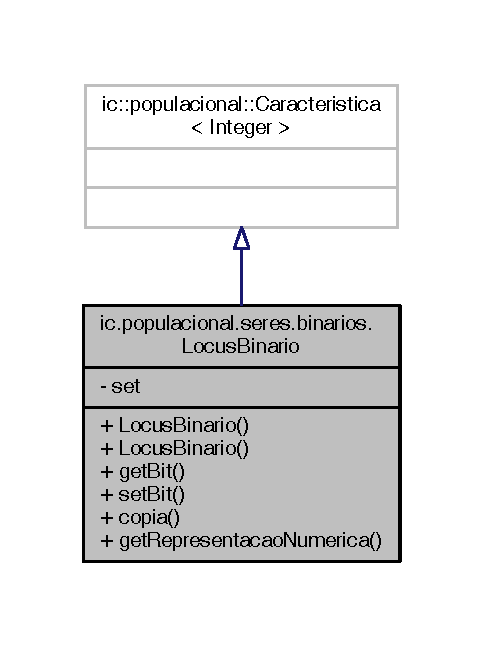
\includegraphics[width=232pt]{classic_1_1populacional_1_1seres_1_1binarios_1_1_locus_binario__inherit__graph}
\end{center}
\end{figure}


Diagrama de colaboração para ic.\-populacional.\-seres.\-binarios.\-Locus\-Binario\-:
\nopagebreak
\begin{figure}[H]
\begin{center}
\leavevmode
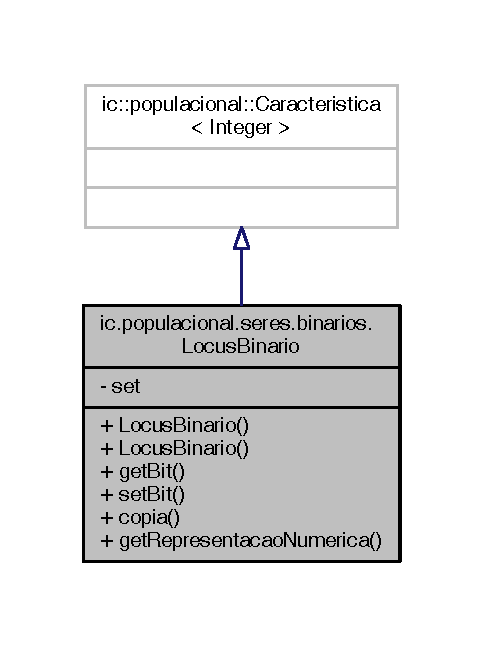
\includegraphics[width=232pt]{classic_1_1populacional_1_1seres_1_1binarios_1_1_locus_binario__coll__graph}
\end{center}
\end{figure}
\subsection*{Métodos Públicos}
\begin{DoxyCompactItemize}
\item 
\hyperlink{classic_1_1populacional_1_1seres_1_1binarios_1_1_locus_binario_a6b51af0fcba0ee9a574f2ec0e2db1b24}{Locus\-Binario} ()
\item 
\hyperlink{classic_1_1populacional_1_1seres_1_1binarios_1_1_locus_binario_aae04767ee00bd5c01de5bc024ade604b}{Locus\-Binario} (boolean \hyperlink{classic_1_1populacional_1_1seres_1_1binarios_1_1_locus_binario_abf7737f18e4a6602f7efdbdfa40d0bf7}{set})
\item 
boolean \hyperlink{classic_1_1populacional_1_1seres_1_1binarios_1_1_locus_binario_a0afc88c8a85163f632005affcabf2723}{get\-Bit} ()
\item 
void \hyperlink{classic_1_1populacional_1_1seres_1_1binarios_1_1_locus_binario_a3534e43918842ff4ccb48279d51fb80a}{set\-Bit} (Boolean bit)
\item 
Caracteristica \hyperlink{classic_1_1populacional_1_1seres_1_1binarios_1_1_locus_binario_a6446b59f5c5c3bf36db3fde5eda1d522}{copia} ()
\item 
Integer \hyperlink{classic_1_1populacional_1_1seres_1_1binarios_1_1_locus_binario_a39e4340f584dd0710e44f044c45d0417}{get\-Representacao\-Numerica} ()
\end{DoxyCompactItemize}
\subsection*{Atributos Privados}
\begin{DoxyCompactItemize}
\item 
boolean \hyperlink{classic_1_1populacional_1_1seres_1_1binarios_1_1_locus_binario_abf7737f18e4a6602f7efdbdfa40d0bf7}{set}
\end{DoxyCompactItemize}


\subsection{Descrição Detalhada}
\begin{DoxyAuthor}{Autor}
Victor de Lima Soares 
\end{DoxyAuthor}


\subsection{Construtores \& Destrutores}
\hypertarget{classic_1_1populacional_1_1seres_1_1binarios_1_1_locus_binario_a6b51af0fcba0ee9a574f2ec0e2db1b24}{\index{ic\-::populacional\-::seres\-::binarios\-::\-Locus\-Binario@{ic\-::populacional\-::seres\-::binarios\-::\-Locus\-Binario}!Locus\-Binario@{Locus\-Binario}}
\index{Locus\-Binario@{Locus\-Binario}!ic::populacional::seres::binarios::LocusBinario@{ic\-::populacional\-::seres\-::binarios\-::\-Locus\-Binario}}
\subsubsection[{Locus\-Binario}]{\setlength{\rightskip}{0pt plus 5cm}ic.\-populacional.\-seres.\-binarios.\-Locus\-Binario.\-Locus\-Binario (
\begin{DoxyParamCaption}
{}
\end{DoxyParamCaption}
)}}\label{classic_1_1populacional_1_1seres_1_1binarios_1_1_locus_binario_a6b51af0fcba0ee9a574f2ec0e2db1b24}


Este é o diagrama das funções que utilizam esta função\-:
\nopagebreak
\begin{figure}[H]
\begin{center}
\leavevmode
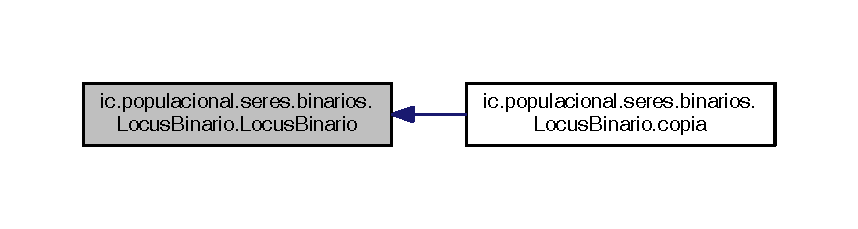
\includegraphics[width=350pt]{classic_1_1populacional_1_1seres_1_1binarios_1_1_locus_binario_a6b51af0fcba0ee9a574f2ec0e2db1b24_icgraph}
\end{center}
\end{figure}


\hypertarget{classic_1_1populacional_1_1seres_1_1binarios_1_1_locus_binario_aae04767ee00bd5c01de5bc024ade604b}{\index{ic\-::populacional\-::seres\-::binarios\-::\-Locus\-Binario@{ic\-::populacional\-::seres\-::binarios\-::\-Locus\-Binario}!Locus\-Binario@{Locus\-Binario}}
\index{Locus\-Binario@{Locus\-Binario}!ic::populacional::seres::binarios::LocusBinario@{ic\-::populacional\-::seres\-::binarios\-::\-Locus\-Binario}}
\subsubsection[{Locus\-Binario}]{\setlength{\rightskip}{0pt plus 5cm}ic.\-populacional.\-seres.\-binarios.\-Locus\-Binario.\-Locus\-Binario (
\begin{DoxyParamCaption}
\item[{boolean}]{set}
\end{DoxyParamCaption}
)}}\label{classic_1_1populacional_1_1seres_1_1binarios_1_1_locus_binario_aae04767ee00bd5c01de5bc024ade604b}


\subsection{Métodos}
\hypertarget{classic_1_1populacional_1_1seres_1_1binarios_1_1_locus_binario_a6446b59f5c5c3bf36db3fde5eda1d522}{\index{ic\-::populacional\-::seres\-::binarios\-::\-Locus\-Binario@{ic\-::populacional\-::seres\-::binarios\-::\-Locus\-Binario}!copia@{copia}}
\index{copia@{copia}!ic::populacional::seres::binarios::LocusBinario@{ic\-::populacional\-::seres\-::binarios\-::\-Locus\-Binario}}
\subsubsection[{copia}]{\setlength{\rightskip}{0pt plus 5cm}Caracteristica ic.\-populacional.\-seres.\-binarios.\-Locus\-Binario.\-copia (
\begin{DoxyParamCaption}
{}
\end{DoxyParamCaption}
)}}\label{classic_1_1populacional_1_1seres_1_1binarios_1_1_locus_binario_a6446b59f5c5c3bf36db3fde5eda1d522}


Este é o diagrama das funções utilizadas por esta função\-:
\nopagebreak
\begin{figure}[H]
\begin{center}
\leavevmode
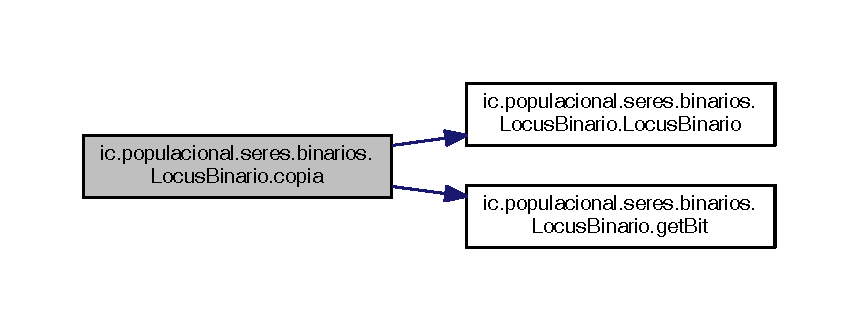
\includegraphics[width=350pt]{classic_1_1populacional_1_1seres_1_1binarios_1_1_locus_binario_a6446b59f5c5c3bf36db3fde5eda1d522_cgraph}
\end{center}
\end{figure}


\hypertarget{classic_1_1populacional_1_1seres_1_1binarios_1_1_locus_binario_a0afc88c8a85163f632005affcabf2723}{\index{ic\-::populacional\-::seres\-::binarios\-::\-Locus\-Binario@{ic\-::populacional\-::seres\-::binarios\-::\-Locus\-Binario}!get\-Bit@{get\-Bit}}
\index{get\-Bit@{get\-Bit}!ic::populacional::seres::binarios::LocusBinario@{ic\-::populacional\-::seres\-::binarios\-::\-Locus\-Binario}}
\subsubsection[{get\-Bit}]{\setlength{\rightskip}{0pt plus 5cm}boolean ic.\-populacional.\-seres.\-binarios.\-Locus\-Binario.\-get\-Bit (
\begin{DoxyParamCaption}
{}
\end{DoxyParamCaption}
)}}\label{classic_1_1populacional_1_1seres_1_1binarios_1_1_locus_binario_a0afc88c8a85163f632005affcabf2723}


Este é o diagrama das funções que utilizam esta função\-:
\nopagebreak
\begin{figure}[H]
\begin{center}
\leavevmode
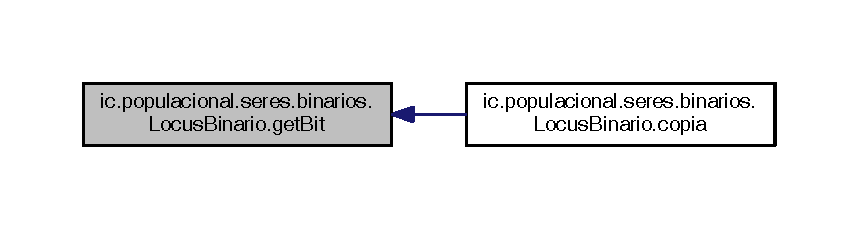
\includegraphics[width=350pt]{classic_1_1populacional_1_1seres_1_1binarios_1_1_locus_binario_a0afc88c8a85163f632005affcabf2723_icgraph}
\end{center}
\end{figure}


\hypertarget{classic_1_1populacional_1_1seres_1_1binarios_1_1_locus_binario_a39e4340f584dd0710e44f044c45d0417}{\index{ic\-::populacional\-::seres\-::binarios\-::\-Locus\-Binario@{ic\-::populacional\-::seres\-::binarios\-::\-Locus\-Binario}!get\-Representacao\-Numerica@{get\-Representacao\-Numerica}}
\index{get\-Representacao\-Numerica@{get\-Representacao\-Numerica}!ic::populacional::seres::binarios::LocusBinario@{ic\-::populacional\-::seres\-::binarios\-::\-Locus\-Binario}}
\subsubsection[{get\-Representacao\-Numerica}]{\setlength{\rightskip}{0pt plus 5cm}Integer ic.\-populacional.\-seres.\-binarios.\-Locus\-Binario.\-get\-Representacao\-Numerica (
\begin{DoxyParamCaption}
{}
\end{DoxyParamCaption}
)}}\label{classic_1_1populacional_1_1seres_1_1binarios_1_1_locus_binario_a39e4340f584dd0710e44f044c45d0417}
\hypertarget{classic_1_1populacional_1_1seres_1_1binarios_1_1_locus_binario_a3534e43918842ff4ccb48279d51fb80a}{\index{ic\-::populacional\-::seres\-::binarios\-::\-Locus\-Binario@{ic\-::populacional\-::seres\-::binarios\-::\-Locus\-Binario}!set\-Bit@{set\-Bit}}
\index{set\-Bit@{set\-Bit}!ic::populacional::seres::binarios::LocusBinario@{ic\-::populacional\-::seres\-::binarios\-::\-Locus\-Binario}}
\subsubsection[{set\-Bit}]{\setlength{\rightskip}{0pt plus 5cm}void ic.\-populacional.\-seres.\-binarios.\-Locus\-Binario.\-set\-Bit (
\begin{DoxyParamCaption}
\item[{Boolean}]{bit}
\end{DoxyParamCaption}
)}}\label{classic_1_1populacional_1_1seres_1_1binarios_1_1_locus_binario_a3534e43918842ff4ccb48279d51fb80a}


\subsection{Atributos}
\hypertarget{classic_1_1populacional_1_1seres_1_1binarios_1_1_locus_binario_abf7737f18e4a6602f7efdbdfa40d0bf7}{\index{ic\-::populacional\-::seres\-::binarios\-::\-Locus\-Binario@{ic\-::populacional\-::seres\-::binarios\-::\-Locus\-Binario}!set@{set}}
\index{set@{set}!ic::populacional::seres::binarios::LocusBinario@{ic\-::populacional\-::seres\-::binarios\-::\-Locus\-Binario}}
\subsubsection[{set}]{\setlength{\rightskip}{0pt plus 5cm}boolean ic.\-populacional.\-seres.\-binarios.\-Locus\-Binario.\-set\hspace{0.3cm}{\ttfamily [private]}}}\label{classic_1_1populacional_1_1seres_1_1binarios_1_1_locus_binario_abf7737f18e4a6602f7efdbdfa40d0bf7}


A documentação para esta classe foi gerada a partir do seguinte arquivo\-:\begin{DoxyCompactItemize}
\item 
C\-:/\-Users/\-Victor/workplace/\-Net\-Beans\-Projects/\-Inteligencia Computacional/src/ic/populacional/seres/binarios/\hyperlink{_locus_binario_8java}{Locus\-Binario.\-java}\end{DoxyCompactItemize}

\hypertarget{classic_1_1populacional_1_1seres_1_1permutacoes_1_1_locus_permutacao}{\section{Referência da Classe ic.\-populacional.\-seres.\-permutacoes.\-Locus\-Permutacao}
\label{classic_1_1populacional_1_1seres_1_1permutacoes_1_1_locus_permutacao}\index{ic.\-populacional.\-seres.\-permutacoes.\-Locus\-Permutacao@{ic.\-populacional.\-seres.\-permutacoes.\-Locus\-Permutacao}}
}


Diagrama de Hierarquia para ic.\-populacional.\-seres.\-permutacoes.\-Locus\-Permutacao\-:
\nopagebreak
\begin{figure}[H]
\begin{center}
\leavevmode
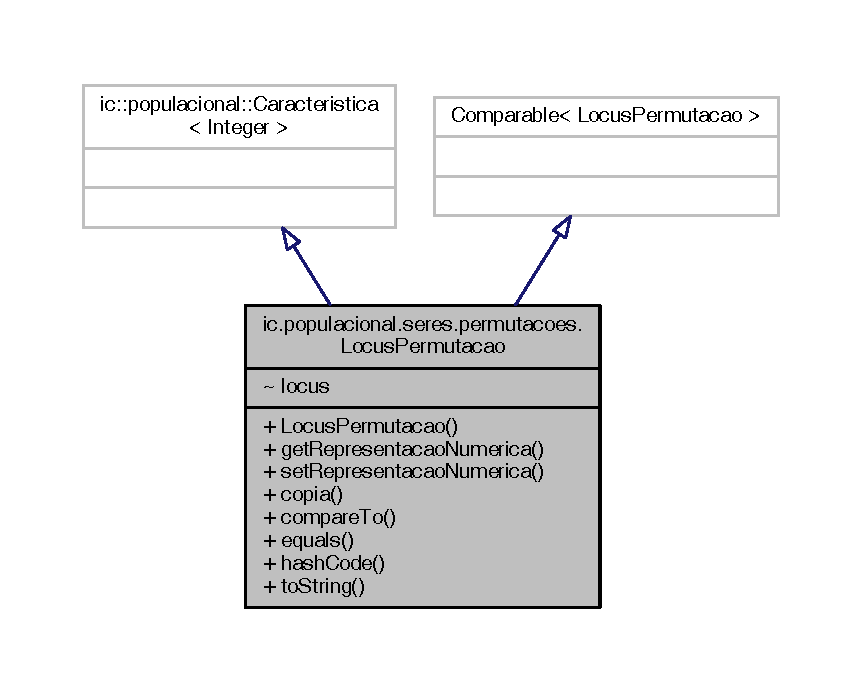
\includegraphics[width=350pt]{classic_1_1populacional_1_1seres_1_1permutacoes_1_1_locus_permutacao__inherit__graph}
\end{center}
\end{figure}


Diagrama de colaboração para ic.\-populacional.\-seres.\-permutacoes.\-Locus\-Permutacao\-:
\nopagebreak
\begin{figure}[H]
\begin{center}
\leavevmode
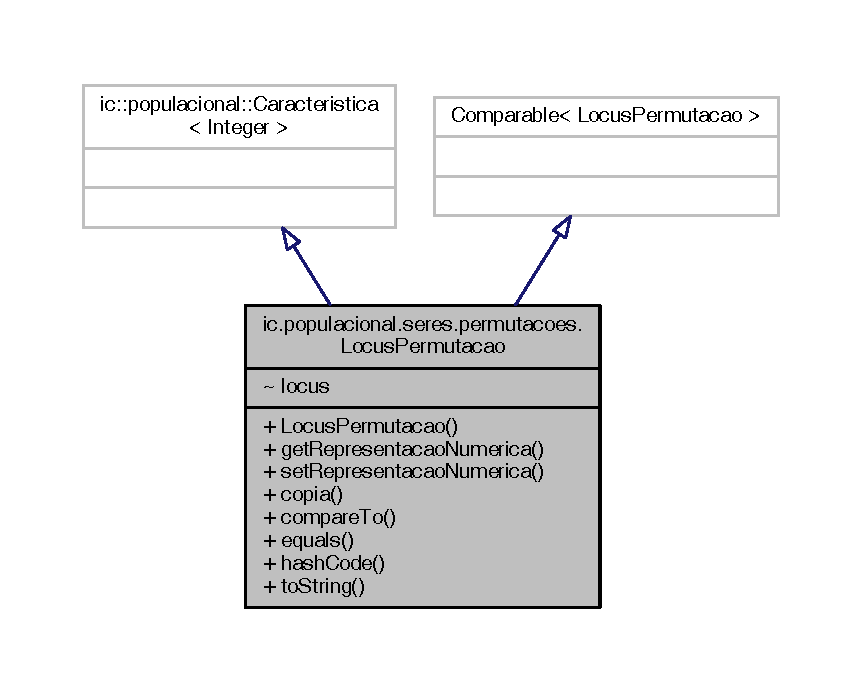
\includegraphics[width=350pt]{classic_1_1populacional_1_1seres_1_1permutacoes_1_1_locus_permutacao__coll__graph}
\end{center}
\end{figure}
\subsection*{Métodos Públicos}
\begin{DoxyCompactItemize}
\item 
\hyperlink{classic_1_1populacional_1_1seres_1_1permutacoes_1_1_locus_permutacao_a07ba9c689e4f7fc03c30e7ef00e8dbf1}{Locus\-Permutacao} (int i)
\item 
Integer \hyperlink{classic_1_1populacional_1_1seres_1_1permutacoes_1_1_locus_permutacao_a849fa3ef6ee79cb3ec71a7323ad131c6}{get\-Representacao\-Numerica} ()
\item 
void \hyperlink{classic_1_1populacional_1_1seres_1_1permutacoes_1_1_locus_permutacao_af563826526caf7402392697602f367be}{set\-Representacao\-Numerica} (int x)
\item 
Caracteristica \hyperlink{classic_1_1populacional_1_1seres_1_1permutacoes_1_1_locus_permutacao_a0745097e35453049b470107363abd6e0}{copia} ()
\item 
int \hyperlink{classic_1_1populacional_1_1seres_1_1permutacoes_1_1_locus_permutacao_acb814e494ea4b3b7b8a9acda72104af8}{compare\-To} (\hyperlink{classic_1_1populacional_1_1seres_1_1permutacoes_1_1_locus_permutacao}{Locus\-Permutacao} o)
\item 
boolean \hyperlink{classic_1_1populacional_1_1seres_1_1permutacoes_1_1_locus_permutacao_ae9e522a0b98639d8dd7c21646a33cc53}{equals} (Object outro)
\item 
int \hyperlink{classic_1_1populacional_1_1seres_1_1permutacoes_1_1_locus_permutacao_af877fffd3f0fd8d0218269ccb7d5e506}{hash\-Code} ()
\item 
String \hyperlink{classic_1_1populacional_1_1seres_1_1permutacoes_1_1_locus_permutacao_ab2d66ef8ea02280c87acad9642892ff7}{to\-String} ()
\end{DoxyCompactItemize}


\subsection{Descrição Detalhada}
\begin{DoxyAuthor}{Autor}
Victor de Lima Soares 
\end{DoxyAuthor}


\subsection{Construtores \& Destrutores}
\hypertarget{classic_1_1populacional_1_1seres_1_1permutacoes_1_1_locus_permutacao_a07ba9c689e4f7fc03c30e7ef00e8dbf1}{\index{ic\-::populacional\-::seres\-::permutacoes\-::\-Locus\-Permutacao@{ic\-::populacional\-::seres\-::permutacoes\-::\-Locus\-Permutacao}!Locus\-Permutacao@{Locus\-Permutacao}}
\index{Locus\-Permutacao@{Locus\-Permutacao}!ic::populacional::seres::permutacoes::LocusPermutacao@{ic\-::populacional\-::seres\-::permutacoes\-::\-Locus\-Permutacao}}
\subsubsection[{Locus\-Permutacao}]{\setlength{\rightskip}{0pt plus 5cm}ic.\-populacional.\-seres.\-permutacoes.\-Locus\-Permutacao.\-Locus\-Permutacao (
\begin{DoxyParamCaption}
\item[{int}]{i}
\end{DoxyParamCaption}
)}}\label{classic_1_1populacional_1_1seres_1_1permutacoes_1_1_locus_permutacao_a07ba9c689e4f7fc03c30e7ef00e8dbf1}


Este é o diagrama das funções que utilizam esta função\-:
\nopagebreak
\begin{figure}[H]
\begin{center}
\leavevmode
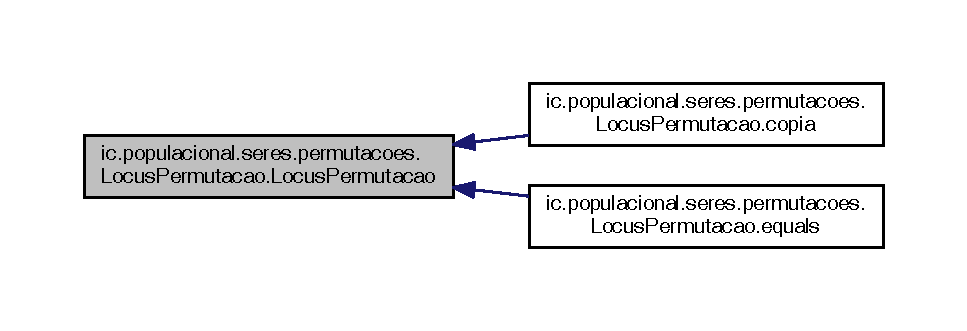
\includegraphics[width=350pt]{classic_1_1populacional_1_1seres_1_1permutacoes_1_1_locus_permutacao_a07ba9c689e4f7fc03c30e7ef00e8dbf1_icgraph}
\end{center}
\end{figure}




\subsection{Métodos}
\hypertarget{classic_1_1populacional_1_1seres_1_1permutacoes_1_1_locus_permutacao_acb814e494ea4b3b7b8a9acda72104af8}{\index{ic\-::populacional\-::seres\-::permutacoes\-::\-Locus\-Permutacao@{ic\-::populacional\-::seres\-::permutacoes\-::\-Locus\-Permutacao}!compare\-To@{compare\-To}}
\index{compare\-To@{compare\-To}!ic::populacional::seres::permutacoes::LocusPermutacao@{ic\-::populacional\-::seres\-::permutacoes\-::\-Locus\-Permutacao}}
\subsubsection[{compare\-To}]{\setlength{\rightskip}{0pt plus 5cm}int ic.\-populacional.\-seres.\-permutacoes.\-Locus\-Permutacao.\-compare\-To (
\begin{DoxyParamCaption}
\item[{{\bf Locus\-Permutacao}}]{o}
\end{DoxyParamCaption}
)}}\label{classic_1_1populacional_1_1seres_1_1permutacoes_1_1_locus_permutacao_acb814e494ea4b3b7b8a9acda72104af8}
\hypertarget{classic_1_1populacional_1_1seres_1_1permutacoes_1_1_locus_permutacao_a0745097e35453049b470107363abd6e0}{\index{ic\-::populacional\-::seres\-::permutacoes\-::\-Locus\-Permutacao@{ic\-::populacional\-::seres\-::permutacoes\-::\-Locus\-Permutacao}!copia@{copia}}
\index{copia@{copia}!ic::populacional::seres::permutacoes::LocusPermutacao@{ic\-::populacional\-::seres\-::permutacoes\-::\-Locus\-Permutacao}}
\subsubsection[{copia}]{\setlength{\rightskip}{0pt plus 5cm}Caracteristica ic.\-populacional.\-seres.\-permutacoes.\-Locus\-Permutacao.\-copia (
\begin{DoxyParamCaption}
{}
\end{DoxyParamCaption}
)}}\label{classic_1_1populacional_1_1seres_1_1permutacoes_1_1_locus_permutacao_a0745097e35453049b470107363abd6e0}


Este é o diagrama das funções utilizadas por esta função\-:
\nopagebreak
\begin{figure}[H]
\begin{center}
\leavevmode
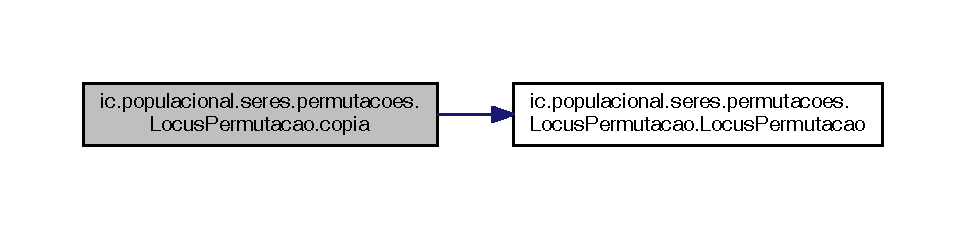
\includegraphics[width=350pt]{classic_1_1populacional_1_1seres_1_1permutacoes_1_1_locus_permutacao_a0745097e35453049b470107363abd6e0_cgraph}
\end{center}
\end{figure}


\hypertarget{classic_1_1populacional_1_1seres_1_1permutacoes_1_1_locus_permutacao_ae9e522a0b98639d8dd7c21646a33cc53}{\index{ic\-::populacional\-::seres\-::permutacoes\-::\-Locus\-Permutacao@{ic\-::populacional\-::seres\-::permutacoes\-::\-Locus\-Permutacao}!equals@{equals}}
\index{equals@{equals}!ic::populacional::seres::permutacoes::LocusPermutacao@{ic\-::populacional\-::seres\-::permutacoes\-::\-Locus\-Permutacao}}
\subsubsection[{equals}]{\setlength{\rightskip}{0pt plus 5cm}boolean ic.\-populacional.\-seres.\-permutacoes.\-Locus\-Permutacao.\-equals (
\begin{DoxyParamCaption}
\item[{Object}]{outro}
\end{DoxyParamCaption}
)}}\label{classic_1_1populacional_1_1seres_1_1permutacoes_1_1_locus_permutacao_ae9e522a0b98639d8dd7c21646a33cc53}


Este é o diagrama das funções utilizadas por esta função\-:
\nopagebreak
\begin{figure}[H]
\begin{center}
\leavevmode
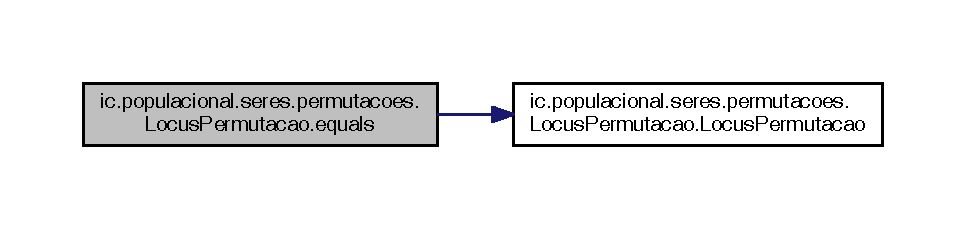
\includegraphics[width=350pt]{classic_1_1populacional_1_1seres_1_1permutacoes_1_1_locus_permutacao_ae9e522a0b98639d8dd7c21646a33cc53_cgraph}
\end{center}
\end{figure}


\hypertarget{classic_1_1populacional_1_1seres_1_1permutacoes_1_1_locus_permutacao_a849fa3ef6ee79cb3ec71a7323ad131c6}{\index{ic\-::populacional\-::seres\-::permutacoes\-::\-Locus\-Permutacao@{ic\-::populacional\-::seres\-::permutacoes\-::\-Locus\-Permutacao}!get\-Representacao\-Numerica@{get\-Representacao\-Numerica}}
\index{get\-Representacao\-Numerica@{get\-Representacao\-Numerica}!ic::populacional::seres::permutacoes::LocusPermutacao@{ic\-::populacional\-::seres\-::permutacoes\-::\-Locus\-Permutacao}}
\subsubsection[{get\-Representacao\-Numerica}]{\setlength{\rightskip}{0pt plus 5cm}Integer ic.\-populacional.\-seres.\-permutacoes.\-Locus\-Permutacao.\-get\-Representacao\-Numerica (
\begin{DoxyParamCaption}
{}
\end{DoxyParamCaption}
)}}\label{classic_1_1populacional_1_1seres_1_1permutacoes_1_1_locus_permutacao_a849fa3ef6ee79cb3ec71a7323ad131c6}
\hypertarget{classic_1_1populacional_1_1seres_1_1permutacoes_1_1_locus_permutacao_af877fffd3f0fd8d0218269ccb7d5e506}{\index{ic\-::populacional\-::seres\-::permutacoes\-::\-Locus\-Permutacao@{ic\-::populacional\-::seres\-::permutacoes\-::\-Locus\-Permutacao}!hash\-Code@{hash\-Code}}
\index{hash\-Code@{hash\-Code}!ic::populacional::seres::permutacoes::LocusPermutacao@{ic\-::populacional\-::seres\-::permutacoes\-::\-Locus\-Permutacao}}
\subsubsection[{hash\-Code}]{\setlength{\rightskip}{0pt plus 5cm}int ic.\-populacional.\-seres.\-permutacoes.\-Locus\-Permutacao.\-hash\-Code (
\begin{DoxyParamCaption}
{}
\end{DoxyParamCaption}
)}}\label{classic_1_1populacional_1_1seres_1_1permutacoes_1_1_locus_permutacao_af877fffd3f0fd8d0218269ccb7d5e506}
\hypertarget{classic_1_1populacional_1_1seres_1_1permutacoes_1_1_locus_permutacao_af563826526caf7402392697602f367be}{\index{ic\-::populacional\-::seres\-::permutacoes\-::\-Locus\-Permutacao@{ic\-::populacional\-::seres\-::permutacoes\-::\-Locus\-Permutacao}!set\-Representacao\-Numerica@{set\-Representacao\-Numerica}}
\index{set\-Representacao\-Numerica@{set\-Representacao\-Numerica}!ic::populacional::seres::permutacoes::LocusPermutacao@{ic\-::populacional\-::seres\-::permutacoes\-::\-Locus\-Permutacao}}
\subsubsection[{set\-Representacao\-Numerica}]{\setlength{\rightskip}{0pt plus 5cm}void ic.\-populacional.\-seres.\-permutacoes.\-Locus\-Permutacao.\-set\-Representacao\-Numerica (
\begin{DoxyParamCaption}
\item[{int}]{x}
\end{DoxyParamCaption}
)}}\label{classic_1_1populacional_1_1seres_1_1permutacoes_1_1_locus_permutacao_af563826526caf7402392697602f367be}
\hypertarget{classic_1_1populacional_1_1seres_1_1permutacoes_1_1_locus_permutacao_ab2d66ef8ea02280c87acad9642892ff7}{\index{ic\-::populacional\-::seres\-::permutacoes\-::\-Locus\-Permutacao@{ic\-::populacional\-::seres\-::permutacoes\-::\-Locus\-Permutacao}!to\-String@{to\-String}}
\index{to\-String@{to\-String}!ic::populacional::seres::permutacoes::LocusPermutacao@{ic\-::populacional\-::seres\-::permutacoes\-::\-Locus\-Permutacao}}
\subsubsection[{to\-String}]{\setlength{\rightskip}{0pt plus 5cm}String ic.\-populacional.\-seres.\-permutacoes.\-Locus\-Permutacao.\-to\-String (
\begin{DoxyParamCaption}
{}
\end{DoxyParamCaption}
)}}\label{classic_1_1populacional_1_1seres_1_1permutacoes_1_1_locus_permutacao_ab2d66ef8ea02280c87acad9642892ff7}


A documentação para esta classe foi gerada a partir do seguinte arquivo\-:\begin{DoxyCompactItemize}
\item 
C\-:/\-Users/\-Victor/workplace/\-Net\-Beans\-Projects/\-Inteligencia Computacional/src/ic/populacional/seres/permutacoes/\hyperlink{_locus_permutacao_8java}{Locus\-Permutacao.\-java}\end{DoxyCompactItemize}

\hypertarget{classic_1_1populacional_1_1seres_1_1reais_1_1_locus_real}{\section{Referência da Classe ic.\-populacional.\-seres.\-reais.\-Locus\-Real}
\label{classic_1_1populacional_1_1seres_1_1reais_1_1_locus_real}\index{ic.\-populacional.\-seres.\-reais.\-Locus\-Real@{ic.\-populacional.\-seres.\-reais.\-Locus\-Real}}
}


Diagrama de Hierarquia para ic.\-populacional.\-seres.\-reais.\-Locus\-Real\-:
\nopagebreak
\begin{figure}[H]
\begin{center}
\leavevmode
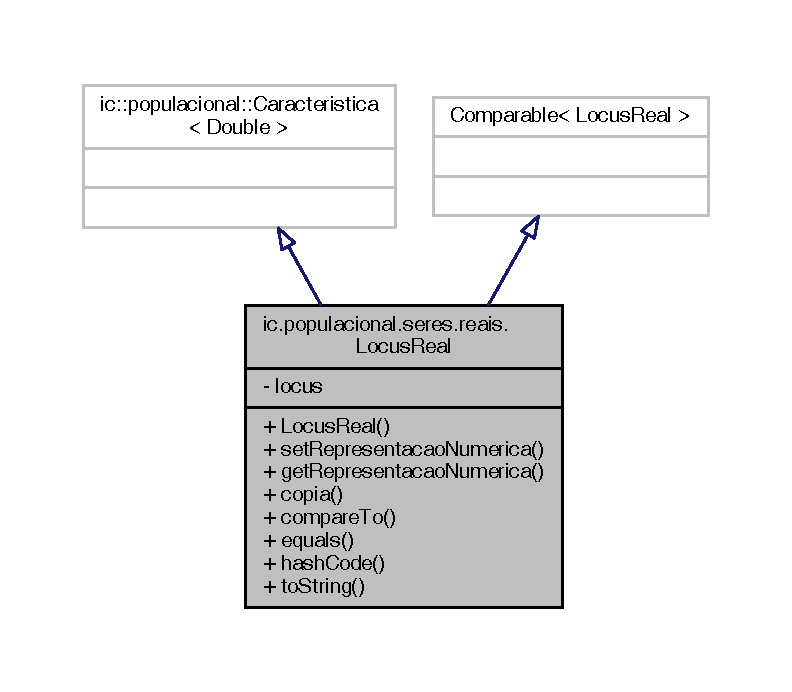
\includegraphics[width=350pt]{classic_1_1populacional_1_1seres_1_1reais_1_1_locus_real__inherit__graph}
\end{center}
\end{figure}


Diagrama de colaboração para ic.\-populacional.\-seres.\-reais.\-Locus\-Real\-:
\nopagebreak
\begin{figure}[H]
\begin{center}
\leavevmode
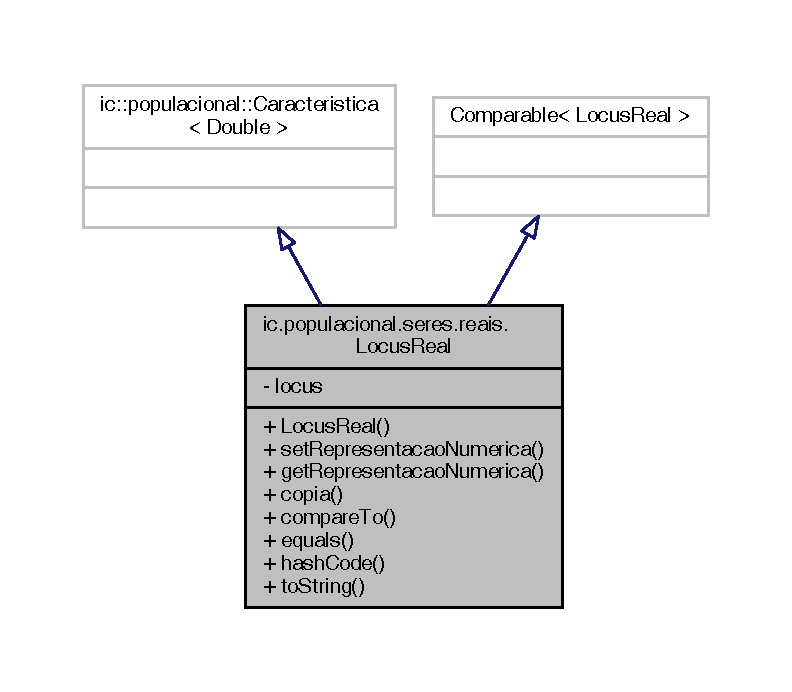
\includegraphics[width=350pt]{classic_1_1populacional_1_1seres_1_1reais_1_1_locus_real__coll__graph}
\end{center}
\end{figure}
\subsection*{Métodos Públicos}
\begin{DoxyCompactItemize}
\item 
\hyperlink{classic_1_1populacional_1_1seres_1_1reais_1_1_locus_real_ae9c9a3cee63ea25176533593e792ce48}{Locus\-Real} (Double \hyperlink{classic_1_1populacional_1_1seres_1_1reais_1_1_locus_real_ab9bbb0e0be3c34b0d7c9249cfc07e377}{locus})
\item 
void \hyperlink{classic_1_1populacional_1_1seres_1_1reais_1_1_locus_real_af38534fbb68bb4e9970f74e505a55d04}{set\-Representacao\-Numerica} (Double \hyperlink{classic_1_1populacional_1_1seres_1_1reais_1_1_locus_real_ab9bbb0e0be3c34b0d7c9249cfc07e377}{locus})
\item 
Double \hyperlink{classic_1_1populacional_1_1seres_1_1reais_1_1_locus_real_a255056872ede5cd634bf87c244a1df19}{get\-Representacao\-Numerica} ()
\item 
Caracteristica \hyperlink{classic_1_1populacional_1_1seres_1_1reais_1_1_locus_real_ae92c0a2f11eef616f08d958a6a58156a}{copia} ()
\item 
int \hyperlink{classic_1_1populacional_1_1seres_1_1reais_1_1_locus_real_af6150465c5ceb87ddb85ccdc85cf0f07}{compare\-To} (\hyperlink{classic_1_1populacional_1_1seres_1_1reais_1_1_locus_real}{Locus\-Real} o)
\item 
boolean \hyperlink{classic_1_1populacional_1_1seres_1_1reais_1_1_locus_real_adef2cb8b1666acb1ca4996a9e322f9e0}{equals} (Object outro)
\item 
int \hyperlink{classic_1_1populacional_1_1seres_1_1reais_1_1_locus_real_a7a9e174b09343b5b4cfc78ca69038ae5}{hash\-Code} ()
\item 
String \hyperlink{classic_1_1populacional_1_1seres_1_1reais_1_1_locus_real_aecf0b483791ecc5a9ecb5f0442e3d18e}{to\-String} ()
\end{DoxyCompactItemize}
\subsection*{Atributos Privados}
\begin{DoxyCompactItemize}
\item 
Double \hyperlink{classic_1_1populacional_1_1seres_1_1reais_1_1_locus_real_ab9bbb0e0be3c34b0d7c9249cfc07e377}{locus}
\end{DoxyCompactItemize}


\subsection{Descrição Detalhada}
\begin{DoxyAuthor}{Autor}
Victor de Lima Soares 
\end{DoxyAuthor}


\subsection{Construtores \& Destrutores}
\hypertarget{classic_1_1populacional_1_1seres_1_1reais_1_1_locus_real_ae9c9a3cee63ea25176533593e792ce48}{\index{ic\-::populacional\-::seres\-::reais\-::\-Locus\-Real@{ic\-::populacional\-::seres\-::reais\-::\-Locus\-Real}!Locus\-Real@{Locus\-Real}}
\index{Locus\-Real@{Locus\-Real}!ic::populacional::seres::reais::LocusReal@{ic\-::populacional\-::seres\-::reais\-::\-Locus\-Real}}
\subsubsection[{Locus\-Real}]{\setlength{\rightskip}{0pt plus 5cm}ic.\-populacional.\-seres.\-reais.\-Locus\-Real.\-Locus\-Real (
\begin{DoxyParamCaption}
\item[{Double}]{locus}
\end{DoxyParamCaption}
)}}\label{classic_1_1populacional_1_1seres_1_1reais_1_1_locus_real_ae9c9a3cee63ea25176533593e792ce48}


Este é o diagrama das funções que utilizam esta função\-:
\nopagebreak
\begin{figure}[H]
\begin{center}
\leavevmode
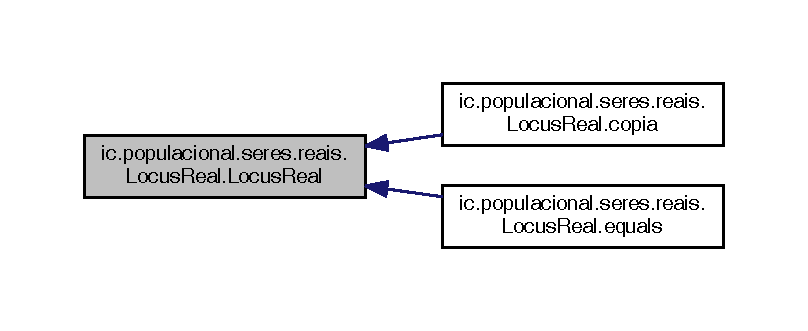
\includegraphics[width=350pt]{classic_1_1populacional_1_1seres_1_1reais_1_1_locus_real_ae9c9a3cee63ea25176533593e792ce48_icgraph}
\end{center}
\end{figure}




\subsection{Métodos}
\hypertarget{classic_1_1populacional_1_1seres_1_1reais_1_1_locus_real_af6150465c5ceb87ddb85ccdc85cf0f07}{\index{ic\-::populacional\-::seres\-::reais\-::\-Locus\-Real@{ic\-::populacional\-::seres\-::reais\-::\-Locus\-Real}!compare\-To@{compare\-To}}
\index{compare\-To@{compare\-To}!ic::populacional::seres::reais::LocusReal@{ic\-::populacional\-::seres\-::reais\-::\-Locus\-Real}}
\subsubsection[{compare\-To}]{\setlength{\rightskip}{0pt plus 5cm}int ic.\-populacional.\-seres.\-reais.\-Locus\-Real.\-compare\-To (
\begin{DoxyParamCaption}
\item[{{\bf Locus\-Real}}]{o}
\end{DoxyParamCaption}
)}}\label{classic_1_1populacional_1_1seres_1_1reais_1_1_locus_real_af6150465c5ceb87ddb85ccdc85cf0f07}
\hypertarget{classic_1_1populacional_1_1seres_1_1reais_1_1_locus_real_ae92c0a2f11eef616f08d958a6a58156a}{\index{ic\-::populacional\-::seres\-::reais\-::\-Locus\-Real@{ic\-::populacional\-::seres\-::reais\-::\-Locus\-Real}!copia@{copia}}
\index{copia@{copia}!ic::populacional::seres::reais::LocusReal@{ic\-::populacional\-::seres\-::reais\-::\-Locus\-Real}}
\subsubsection[{copia}]{\setlength{\rightskip}{0pt plus 5cm}Caracteristica ic.\-populacional.\-seres.\-reais.\-Locus\-Real.\-copia (
\begin{DoxyParamCaption}
{}
\end{DoxyParamCaption}
)}}\label{classic_1_1populacional_1_1seres_1_1reais_1_1_locus_real_ae92c0a2f11eef616f08d958a6a58156a}


Este é o diagrama das funções utilizadas por esta função\-:
\nopagebreak
\begin{figure}[H]
\begin{center}
\leavevmode
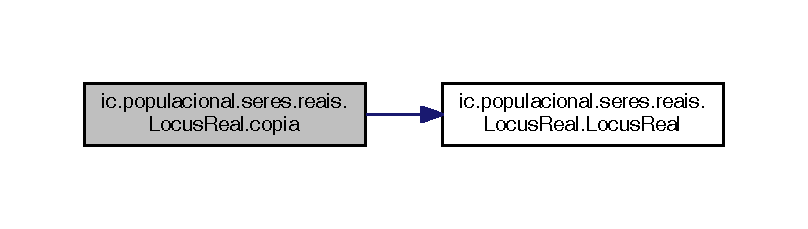
\includegraphics[width=350pt]{classic_1_1populacional_1_1seres_1_1reais_1_1_locus_real_ae92c0a2f11eef616f08d958a6a58156a_cgraph}
\end{center}
\end{figure}


\hypertarget{classic_1_1populacional_1_1seres_1_1reais_1_1_locus_real_adef2cb8b1666acb1ca4996a9e322f9e0}{\index{ic\-::populacional\-::seres\-::reais\-::\-Locus\-Real@{ic\-::populacional\-::seres\-::reais\-::\-Locus\-Real}!equals@{equals}}
\index{equals@{equals}!ic::populacional::seres::reais::LocusReal@{ic\-::populacional\-::seres\-::reais\-::\-Locus\-Real}}
\subsubsection[{equals}]{\setlength{\rightskip}{0pt plus 5cm}boolean ic.\-populacional.\-seres.\-reais.\-Locus\-Real.\-equals (
\begin{DoxyParamCaption}
\item[{Object}]{outro}
\end{DoxyParamCaption}
)}}\label{classic_1_1populacional_1_1seres_1_1reais_1_1_locus_real_adef2cb8b1666acb1ca4996a9e322f9e0}


Este é o diagrama das funções utilizadas por esta função\-:
\nopagebreak
\begin{figure}[H]
\begin{center}
\leavevmode
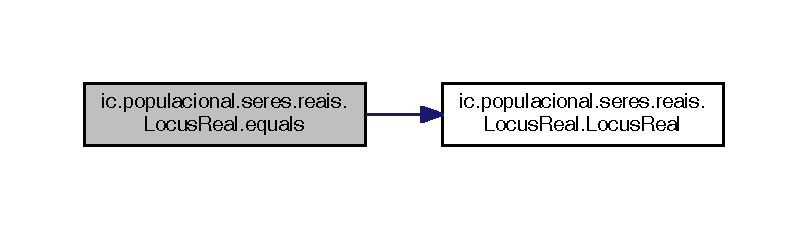
\includegraphics[width=350pt]{classic_1_1populacional_1_1seres_1_1reais_1_1_locus_real_adef2cb8b1666acb1ca4996a9e322f9e0_cgraph}
\end{center}
\end{figure}


\hypertarget{classic_1_1populacional_1_1seres_1_1reais_1_1_locus_real_a255056872ede5cd634bf87c244a1df19}{\index{ic\-::populacional\-::seres\-::reais\-::\-Locus\-Real@{ic\-::populacional\-::seres\-::reais\-::\-Locus\-Real}!get\-Representacao\-Numerica@{get\-Representacao\-Numerica}}
\index{get\-Representacao\-Numerica@{get\-Representacao\-Numerica}!ic::populacional::seres::reais::LocusReal@{ic\-::populacional\-::seres\-::reais\-::\-Locus\-Real}}
\subsubsection[{get\-Representacao\-Numerica}]{\setlength{\rightskip}{0pt plus 5cm}Double ic.\-populacional.\-seres.\-reais.\-Locus\-Real.\-get\-Representacao\-Numerica (
\begin{DoxyParamCaption}
{}
\end{DoxyParamCaption}
)}}\label{classic_1_1populacional_1_1seres_1_1reais_1_1_locus_real_a255056872ede5cd634bf87c244a1df19}
\hypertarget{classic_1_1populacional_1_1seres_1_1reais_1_1_locus_real_a7a9e174b09343b5b4cfc78ca69038ae5}{\index{ic\-::populacional\-::seres\-::reais\-::\-Locus\-Real@{ic\-::populacional\-::seres\-::reais\-::\-Locus\-Real}!hash\-Code@{hash\-Code}}
\index{hash\-Code@{hash\-Code}!ic::populacional::seres::reais::LocusReal@{ic\-::populacional\-::seres\-::reais\-::\-Locus\-Real}}
\subsubsection[{hash\-Code}]{\setlength{\rightskip}{0pt plus 5cm}int ic.\-populacional.\-seres.\-reais.\-Locus\-Real.\-hash\-Code (
\begin{DoxyParamCaption}
{}
\end{DoxyParamCaption}
)}}\label{classic_1_1populacional_1_1seres_1_1reais_1_1_locus_real_a7a9e174b09343b5b4cfc78ca69038ae5}
\hypertarget{classic_1_1populacional_1_1seres_1_1reais_1_1_locus_real_af38534fbb68bb4e9970f74e505a55d04}{\index{ic\-::populacional\-::seres\-::reais\-::\-Locus\-Real@{ic\-::populacional\-::seres\-::reais\-::\-Locus\-Real}!set\-Representacao\-Numerica@{set\-Representacao\-Numerica}}
\index{set\-Representacao\-Numerica@{set\-Representacao\-Numerica}!ic::populacional::seres::reais::LocusReal@{ic\-::populacional\-::seres\-::reais\-::\-Locus\-Real}}
\subsubsection[{set\-Representacao\-Numerica}]{\setlength{\rightskip}{0pt plus 5cm}void ic.\-populacional.\-seres.\-reais.\-Locus\-Real.\-set\-Representacao\-Numerica (
\begin{DoxyParamCaption}
\item[{Double}]{locus}
\end{DoxyParamCaption}
)}}\label{classic_1_1populacional_1_1seres_1_1reais_1_1_locus_real_af38534fbb68bb4e9970f74e505a55d04}
\hypertarget{classic_1_1populacional_1_1seres_1_1reais_1_1_locus_real_aecf0b483791ecc5a9ecb5f0442e3d18e}{\index{ic\-::populacional\-::seres\-::reais\-::\-Locus\-Real@{ic\-::populacional\-::seres\-::reais\-::\-Locus\-Real}!to\-String@{to\-String}}
\index{to\-String@{to\-String}!ic::populacional::seres::reais::LocusReal@{ic\-::populacional\-::seres\-::reais\-::\-Locus\-Real}}
\subsubsection[{to\-String}]{\setlength{\rightskip}{0pt plus 5cm}String ic.\-populacional.\-seres.\-reais.\-Locus\-Real.\-to\-String (
\begin{DoxyParamCaption}
{}
\end{DoxyParamCaption}
)}}\label{classic_1_1populacional_1_1seres_1_1reais_1_1_locus_real_aecf0b483791ecc5a9ecb5f0442e3d18e}


\subsection{Atributos}
\hypertarget{classic_1_1populacional_1_1seres_1_1reais_1_1_locus_real_ab9bbb0e0be3c34b0d7c9249cfc07e377}{\index{ic\-::populacional\-::seres\-::reais\-::\-Locus\-Real@{ic\-::populacional\-::seres\-::reais\-::\-Locus\-Real}!locus@{locus}}
\index{locus@{locus}!ic::populacional::seres::reais::LocusReal@{ic\-::populacional\-::seres\-::reais\-::\-Locus\-Real}}
\subsubsection[{locus}]{\setlength{\rightskip}{0pt plus 5cm}Double ic.\-populacional.\-seres.\-reais.\-Locus\-Real.\-locus\hspace{0.3cm}{\ttfamily [private]}}}\label{classic_1_1populacional_1_1seres_1_1reais_1_1_locus_real_ab9bbb0e0be3c34b0d7c9249cfc07e377}


A documentação para esta classe foi gerada a partir do seguinte arquivo\-:\begin{DoxyCompactItemize}
\item 
C\-:/\-Users/\-Victor/workplace/\-Net\-Beans\-Projects/\-Inteligencia Computacional/src/ic/populacional/seres/reais/\hyperlink{_locus_real_8java}{Locus\-Real.\-java}\end{DoxyCompactItemize}

\hypertarget{enumic_1_1populacional_1_1_ambiente_3_01_g_01extends_01_number_01_6_comparable_3_01_g_01_4_00_0156fb2ffb0f78f5b655aaee5b0df471a7}{\section{ic.\-populacional.\-Ambiente$<$ G extends Number \&Comparable$<$ G $>$, S extends Ser$<$ G $>$ $>$.Modo Enum Reference}
\label{enumic_1_1populacional_1_1_ambiente_3_01_g_01extends_01_number_01_6_comparable_3_01_g_01_4_00_0156fb2ffb0f78f5b655aaee5b0df471a7}\index{ic.\-populacional.\-Ambiente$<$ G extends Number \&\-Comparable$<$ G $>$, S extends Ser$<$ G $>$ $>$.\-Modo@{ic.\-populacional.\-Ambiente$<$ G extends Number \&\-Comparable$<$ G $>$, S extends Ser$<$ G $>$ $>$.\-Modo}}
}


Defini o modo de comparação entre os seres.  




Diagrama de colaboração para ic.\-populacional.\-Ambiente$<$ G extends Number \&Comparable$<$ G $>$, S extends Ser$<$ G $>$ $>$.Modo\-:
\nopagebreak
\begin{figure}[H]
\begin{center}
\leavevmode
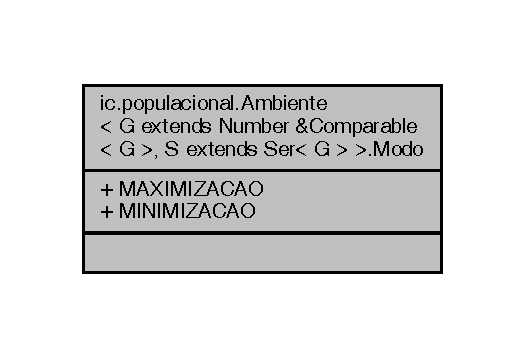
\includegraphics[width=252pt]{enumic_1_1populacional_1_1_ambiente_3_01_g_01extends_01_number_01_6_comparable_3_01_g_01_4_00_013449bdab33fd736a81c080f8d267e888}
\end{center}
\end{figure}
\subsection*{Atributos Públicos}
\begin{DoxyCompactItemize}
\item 
\hyperlink{enumic_1_1populacional_1_1_ambiente_3_01_g_01extends_01_number_01_6_comparable_3_01_g_01_4_00_0156fb2ffb0f78f5b655aaee5b0df471a7_aebd926ba90a2f0976426930757e52389}{M\-A\-X\-I\-M\-I\-Z\-A\-C\-A\-O}
\item 
\hyperlink{enumic_1_1populacional_1_1_ambiente_3_01_g_01extends_01_number_01_6_comparable_3_01_g_01_4_00_0156fb2ffb0f78f5b655aaee5b0df471a7_a78ac05db732c05991ffbc586141bd137}{M\-I\-N\-I\-M\-I\-Z\-A\-C\-A\-O}
\end{DoxyCompactItemize}


\subsection{Descrição Detalhada}
Defini o modo de comparação entre os seres. 

Pelo modo, o ambiente será capaz de identificar a ordem correta dos seres ao compará-\/los.

Para problemas de minimização, um ser com menor “grau de adaptação” será melhor e posto após os com maiores graus – em uma ordem crescente. Contudo, para maximização (modo padrão), seres com graus maiores serão considerados melhores e quando ordenados viram após os com menores graus. 

\subsection{Atributos}
\hypertarget{enumic_1_1populacional_1_1_ambiente_3_01_g_01extends_01_number_01_6_comparable_3_01_g_01_4_00_0156fb2ffb0f78f5b655aaee5b0df471a7_aebd926ba90a2f0976426930757e52389}{\index{ic\-::populacional\-::\-Ambiente$<$ G extends Number \&\-Comparable$<$ G $>$, S extends Ser$<$ G $>$ $>$\-::\-Modo@{ic\-::populacional\-::\-Ambiente$<$ G extends Number \&\-Comparable$<$ G $>$, S extends Ser$<$ G $>$ $>$\-::\-Modo}!M\-A\-X\-I\-M\-I\-Z\-A\-C\-A\-O@{M\-A\-X\-I\-M\-I\-Z\-A\-C\-A\-O}}
\index{M\-A\-X\-I\-M\-I\-Z\-A\-C\-A\-O@{M\-A\-X\-I\-M\-I\-Z\-A\-C\-A\-O}!ic::populacional::Ambiente< G extends Number &Comparable< G >, S extends Ser< G > >::Modo@{ic\-::populacional\-::\-Ambiente$<$ G extends Number \&\-Comparable$<$ G $>$, S extends Ser$<$ G $>$ $>$\-::\-Modo}}
\subsubsection[{M\-A\-X\-I\-M\-I\-Z\-A\-C\-A\-O}]{\setlength{\rightskip}{0pt plus 5cm}ic.\-populacional.\-Ambiente$<$ G extends Number \&Comparable$<$ G $>$, S extends Ser$<$ G $>$ $>$.Modo.\-M\-A\-X\-I\-M\-I\-Z\-A\-C\-A\-O}}\label{enumic_1_1populacional_1_1_ambiente_3_01_g_01extends_01_number_01_6_comparable_3_01_g_01_4_00_0156fb2ffb0f78f5b655aaee5b0df471a7_aebd926ba90a2f0976426930757e52389}
\hypertarget{enumic_1_1populacional_1_1_ambiente_3_01_g_01extends_01_number_01_6_comparable_3_01_g_01_4_00_0156fb2ffb0f78f5b655aaee5b0df471a7_a78ac05db732c05991ffbc586141bd137}{\index{ic\-::populacional\-::\-Ambiente$<$ G extends Number \&\-Comparable$<$ G $>$, S extends Ser$<$ G $>$ $>$\-::\-Modo@{ic\-::populacional\-::\-Ambiente$<$ G extends Number \&\-Comparable$<$ G $>$, S extends Ser$<$ G $>$ $>$\-::\-Modo}!M\-I\-N\-I\-M\-I\-Z\-A\-C\-A\-O@{M\-I\-N\-I\-M\-I\-Z\-A\-C\-A\-O}}
\index{M\-I\-N\-I\-M\-I\-Z\-A\-C\-A\-O@{M\-I\-N\-I\-M\-I\-Z\-A\-C\-A\-O}!ic::populacional::Ambiente< G extends Number &Comparable< G >, S extends Ser< G > >::Modo@{ic\-::populacional\-::\-Ambiente$<$ G extends Number \&\-Comparable$<$ G $>$, S extends Ser$<$ G $>$ $>$\-::\-Modo}}
\subsubsection[{M\-I\-N\-I\-M\-I\-Z\-A\-C\-A\-O}]{\setlength{\rightskip}{0pt plus 5cm}ic.\-populacional.\-Ambiente$<$ G extends Number \&Comparable$<$ G $>$, S extends Ser$<$ G $>$ $>$.Modo.\-M\-I\-N\-I\-M\-I\-Z\-A\-C\-A\-O}}\label{enumic_1_1populacional_1_1_ambiente_3_01_g_01extends_01_number_01_6_comparable_3_01_g_01_4_00_0156fb2ffb0f78f5b655aaee5b0df471a7_a78ac05db732c05991ffbc586141bd137}


The documentation for this enum was generated from the following file\-:\begin{DoxyCompactItemize}
\item 
C\-:/\-Users/\-Victor/workplace/\-Net\-Beans\-Projects/\-Inteligencia Computacional/src/ic/populacional/\hyperlink{_ambiente_8java}{Ambiente.\-java}\end{DoxyCompactItemize}

\hypertarget{classic_1_1populacional_1_1algoritmo_1_1operadores_1_1_mutador_3_01_t_01extends_01_ser_01_4}{\section{Referência da Classe ic.\-populacional.\-algoritmo.\-operadores.\-Mutador$<$ T extends Ser $>$}
\label{classic_1_1populacional_1_1algoritmo_1_1operadores_1_1_mutador_3_01_t_01extends_01_ser_01_4}\index{ic.\-populacional.\-algoritmo.\-operadores.\-Mutador$<$ T extends Ser $>$@{ic.\-populacional.\-algoritmo.\-operadores.\-Mutador$<$ T extends Ser $>$}}
}


Diagrama de Hierarquia para ic.\-populacional.\-algoritmo.\-operadores.\-Mutador$<$ T extends Ser $>$\-:
\nopagebreak
\begin{figure}[H]
\begin{center}
\leavevmode
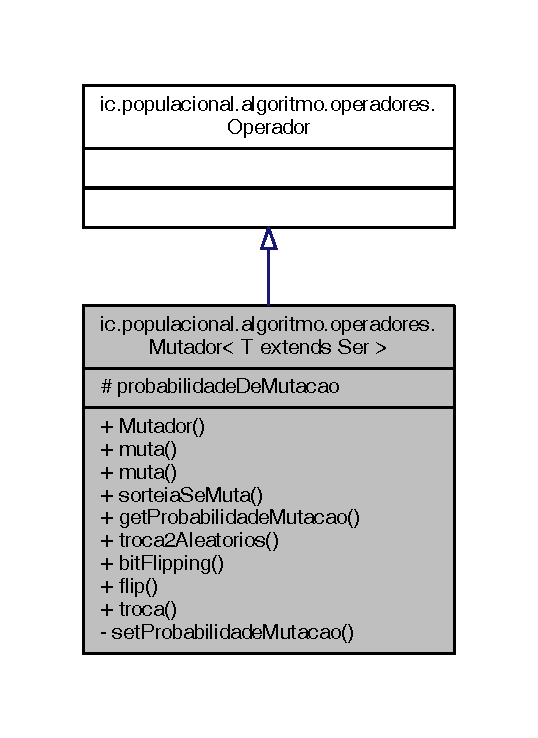
\includegraphics[width=258pt]{classic_1_1populacional_1_1algoritmo_1_1operadores_1_1_mutador_3_01_t_01extends_01_ser_01_4__inherit__graph}
\end{center}
\end{figure}


Diagrama de colaboração para ic.\-populacional.\-algoritmo.\-operadores.\-Mutador$<$ T extends Ser $>$\-:
\nopagebreak
\begin{figure}[H]
\begin{center}
\leavevmode
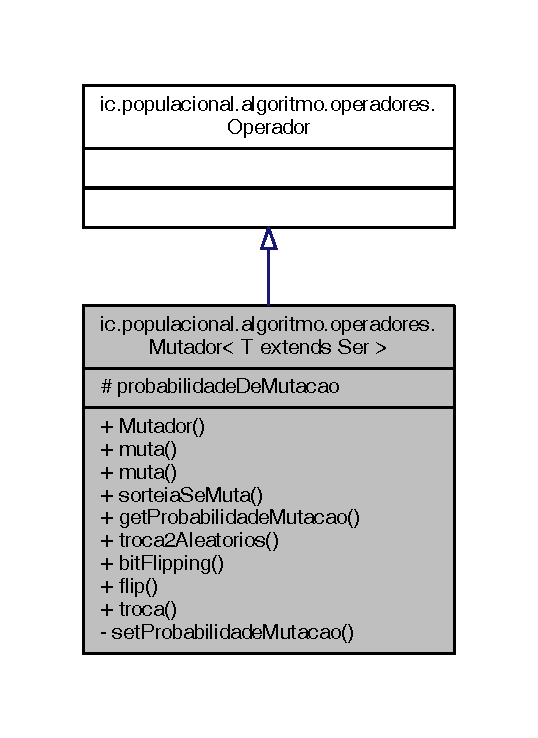
\includegraphics[width=258pt]{classic_1_1populacional_1_1algoritmo_1_1operadores_1_1_mutador_3_01_t_01extends_01_ser_01_4__coll__graph}
\end{center}
\end{figure}
\subsection*{Métodos Públicos}
\begin{DoxyCompactItemize}
\item 
\hyperlink{classic_1_1populacional_1_1algoritmo_1_1operadores_1_1_mutador_3_01_t_01extends_01_ser_01_4_a91f0ac5d3d47ccca5fe3b629bb8db51e}{Mutador} (double \hyperlink{classic_1_1populacional_1_1algoritmo_1_1operadores_1_1_mutador_3_01_t_01extends_01_ser_01_4_a1ef75bbeff32bd2bf0b56c8b2ad86c60}{probabilidade\-De\-Mutacao})
\item 
abstract void \hyperlink{classic_1_1populacional_1_1algoritmo_1_1operadores_1_1_mutador_3_01_t_01extends_01_ser_01_4_a69073efced7c28f34fc78a1406997f68}{muta} (T origem)
\begin{DoxyCompactList}\small\item\em Realiza a operação de mutação. \end{DoxyCompactList}\item 
void \hyperlink{classic_1_1populacional_1_1algoritmo_1_1operadores_1_1_mutador_3_01_t_01extends_01_ser_01_4_a618c8c12d4f4c6fa0a1165b6b255451c}{muta} (Collection$<$ T $>$ seres)
\item 
boolean \hyperlink{classic_1_1populacional_1_1algoritmo_1_1operadores_1_1_mutador_3_01_t_01extends_01_ser_01_4_afd84303577dcfd8bd6bad1f805688413}{sorteia\-Se\-Muta} ()
\item 
final double \hyperlink{classic_1_1populacional_1_1algoritmo_1_1operadores_1_1_mutador_3_01_t_01extends_01_ser_01_4_a2805588bab5915c85a803de4187f6678}{get\-Probabilidade\-Mutacao} ()
\end{DoxyCompactItemize}
\subsection*{Métodos Públicos Estáticos}
\begin{DoxyCompactItemize}
\item 
static final void \hyperlink{classic_1_1populacional_1_1algoritmo_1_1operadores_1_1_mutador_3_01_t_01extends_01_ser_01_4_afbcb2c72a47a82dd94dcfb4295953d88}{troca2\-Aleatorios} (Ser origem)
\begin{DoxyCompactList}\small\item\em Realiza a troca de duas características em um ser, selecionadas aleatoriamente. \end{DoxyCompactList}\item 
static final void \hyperlink{classic_1_1populacional_1_1algoritmo_1_1operadores_1_1_mutador_3_01_t_01extends_01_ser_01_4_aebd2c6138299aa0bb03788702683133b}{bit\-Flipping} (Ser origem, double probabilidade\-De\-Flip)
\begin{DoxyCompactList}\small\item\em bit-\/flipping \end{DoxyCompactList}\item 
static final void \hyperlink{classic_1_1populacional_1_1algoritmo_1_1operadores_1_1_mutador_3_01_t_01extends_01_ser_01_4_a173c08a7e8ae9b3395bb24a801ac593e}{flip} (\hyperlink{classic_1_1populacional_1_1seres_1_1binarios_1_1_caracteristica_binaria}{Caracteristica\-Binaria} locus)
\begin{DoxyCompactList}\small\item\em Realiza a inversão de valor de uma característica binária. \end{DoxyCompactList}\item 
static final void \hyperlink{classic_1_1populacional_1_1algoritmo_1_1operadores_1_1_mutador_3_01_t_01extends_01_ser_01_4_a7a97c38f07d20dcb3bd2c8b83bd64444}{troca} (Ser origem, int indice\-I, int indice\-J)
\begin{DoxyCompactList}\small\item\em Realiza a troca de duas características em um ser. \end{DoxyCompactList}\end{DoxyCompactItemize}
\subsection*{Atributos Protegidos}
\begin{DoxyCompactItemize}
\item 
double \hyperlink{classic_1_1populacional_1_1algoritmo_1_1operadores_1_1_mutador_3_01_t_01extends_01_ser_01_4_a1ef75bbeff32bd2bf0b56c8b2ad86c60}{probabilidade\-De\-Mutacao}
\end{DoxyCompactItemize}
\subsection*{Métodos Privados}
\begin{DoxyCompactItemize}
\item 
final void \hyperlink{classic_1_1populacional_1_1algoritmo_1_1operadores_1_1_mutador_3_01_t_01extends_01_ser_01_4_afcdb84bb1e7461f96a7aa4c817ae8c29}{set\-Probabilidade\-Mutacao} (double probabilidade\-Mutacao)  throws Illegal\-Argument\-Exception 
\end{DoxyCompactItemize}


\subsection{Descrição Detalhada}
\begin{DoxyAuthor}{Autor}
Victor de Lima Soares 
\end{DoxyAuthor}


\subsection{Construtores \& Destrutores}
\hypertarget{classic_1_1populacional_1_1algoritmo_1_1operadores_1_1_mutador_3_01_t_01extends_01_ser_01_4_a91f0ac5d3d47ccca5fe3b629bb8db51e}{\index{ic\-::populacional\-::algoritmo\-::operadores\-::\-Mutador$<$ T extends Ser $>$@{ic\-::populacional\-::algoritmo\-::operadores\-::\-Mutador$<$ T extends Ser $>$}!Mutador@{Mutador}}
\index{Mutador@{Mutador}!ic::populacional::algoritmo::operadores::Mutador< T extends Ser >@{ic\-::populacional\-::algoritmo\-::operadores\-::\-Mutador$<$ T extends Ser $>$}}
\subsubsection[{Mutador}]{\setlength{\rightskip}{0pt plus 5cm}ic.\-populacional.\-algoritmo.\-operadores.\-Mutador$<$ T extends Ser $>$.Mutador (
\begin{DoxyParamCaption}
\item[{double}]{probabilidade\-De\-Mutacao}
\end{DoxyParamCaption}
)}}\label{classic_1_1populacional_1_1algoritmo_1_1operadores_1_1_mutador_3_01_t_01extends_01_ser_01_4_a91f0ac5d3d47ccca5fe3b629bb8db51e}


\subsection{Métodos}
\hypertarget{classic_1_1populacional_1_1algoritmo_1_1operadores_1_1_mutador_3_01_t_01extends_01_ser_01_4_aebd2c6138299aa0bb03788702683133b}{\index{ic\-::populacional\-::algoritmo\-::operadores\-::\-Mutador$<$ T extends Ser $>$@{ic\-::populacional\-::algoritmo\-::operadores\-::\-Mutador$<$ T extends Ser $>$}!bit\-Flipping@{bit\-Flipping}}
\index{bit\-Flipping@{bit\-Flipping}!ic::populacional::algoritmo::operadores::Mutador< T extends Ser >@{ic\-::populacional\-::algoritmo\-::operadores\-::\-Mutador$<$ T extends Ser $>$}}
\subsubsection[{bit\-Flipping}]{\setlength{\rightskip}{0pt plus 5cm}static final void ic.\-populacional.\-algoritmo.\-operadores.\-Mutador$<$ T extends Ser $>$.bit\-Flipping (
\begin{DoxyParamCaption}
\item[{Ser}]{origem, }
\item[{double}]{probabilidade\-De\-Flip}
\end{DoxyParamCaption}
)\hspace{0.3cm}{\ttfamily [static]}}}\label{classic_1_1populacional_1_1algoritmo_1_1operadores_1_1_mutador_3_01_t_01extends_01_ser_01_4_aebd2c6138299aa0bb03788702683133b}


bit-\/flipping 


\begin{DoxyParams}{Parâmetros}
{\em origem} & \\
\hline
{\em probabilidade\-De\-Flip} & \\
\hline
\end{DoxyParams}


Este é o diagrama das funções utilizadas por esta função\-:\nopagebreak
\begin{figure}[H]
\begin{center}
\leavevmode
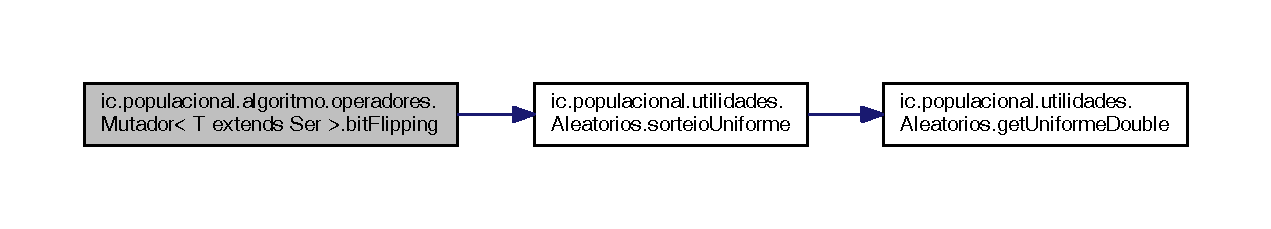
\includegraphics[width=350pt]{classic_1_1populacional_1_1algoritmo_1_1operadores_1_1_mutador_3_01_t_01extends_01_ser_01_4_aebd2c6138299aa0bb03788702683133b_cgraph}
\end{center}
\end{figure}


\hypertarget{classic_1_1populacional_1_1algoritmo_1_1operadores_1_1_mutador_3_01_t_01extends_01_ser_01_4_a173c08a7e8ae9b3395bb24a801ac593e}{\index{ic\-::populacional\-::algoritmo\-::operadores\-::\-Mutador$<$ T extends Ser $>$@{ic\-::populacional\-::algoritmo\-::operadores\-::\-Mutador$<$ T extends Ser $>$}!flip@{flip}}
\index{flip@{flip}!ic::populacional::algoritmo::operadores::Mutador< T extends Ser >@{ic\-::populacional\-::algoritmo\-::operadores\-::\-Mutador$<$ T extends Ser $>$}}
\subsubsection[{flip}]{\setlength{\rightskip}{0pt plus 5cm}static final void ic.\-populacional.\-algoritmo.\-operadores.\-Mutador$<$ T extends Ser $>$.flip (
\begin{DoxyParamCaption}
\item[{{\bf Caracteristica\-Binaria}}]{locus}
\end{DoxyParamCaption}
)\hspace{0.3cm}{\ttfamily [static]}}}\label{classic_1_1populacional_1_1algoritmo_1_1operadores_1_1_mutador_3_01_t_01extends_01_ser_01_4_a173c08a7e8ae9b3395bb24a801ac593e}


Realiza a inversão de valor de uma característica binária. 


\begin{DoxyParams}{Parâmetros}
{\em locus} & Característica binária objeto da mutação.\\
\hline
\end{DoxyParams}
\begin{DoxySince}{Desde}
1.\-0 
\end{DoxySince}
\hypertarget{classic_1_1populacional_1_1algoritmo_1_1operadores_1_1_mutador_3_01_t_01extends_01_ser_01_4_a2805588bab5915c85a803de4187f6678}{\index{ic\-::populacional\-::algoritmo\-::operadores\-::\-Mutador$<$ T extends Ser $>$@{ic\-::populacional\-::algoritmo\-::operadores\-::\-Mutador$<$ T extends Ser $>$}!get\-Probabilidade\-Mutacao@{get\-Probabilidade\-Mutacao}}
\index{get\-Probabilidade\-Mutacao@{get\-Probabilidade\-Mutacao}!ic::populacional::algoritmo::operadores::Mutador< T extends Ser >@{ic\-::populacional\-::algoritmo\-::operadores\-::\-Mutador$<$ T extends Ser $>$}}
\subsubsection[{get\-Probabilidade\-Mutacao}]{\setlength{\rightskip}{0pt plus 5cm}final double ic.\-populacional.\-algoritmo.\-operadores.\-Mutador$<$ T extends Ser $>$.get\-Probabilidade\-Mutacao (
\begin{DoxyParamCaption}
{}
\end{DoxyParamCaption}
)}}\label{classic_1_1populacional_1_1algoritmo_1_1operadores_1_1_mutador_3_01_t_01extends_01_ser_01_4_a2805588bab5915c85a803de4187f6678}
\begin{DoxyReturn}{Retorna}
a probabilidade de mutação. 
\end{DoxyReturn}
\hypertarget{classic_1_1populacional_1_1algoritmo_1_1operadores_1_1_mutador_3_01_t_01extends_01_ser_01_4_a69073efced7c28f34fc78a1406997f68}{\index{ic\-::populacional\-::algoritmo\-::operadores\-::\-Mutador$<$ T extends Ser $>$@{ic\-::populacional\-::algoritmo\-::operadores\-::\-Mutador$<$ T extends Ser $>$}!muta@{muta}}
\index{muta@{muta}!ic::populacional::algoritmo::operadores::Mutador< T extends Ser >@{ic\-::populacional\-::algoritmo\-::operadores\-::\-Mutador$<$ T extends Ser $>$}}
\subsubsection[{muta}]{\setlength{\rightskip}{0pt plus 5cm}abstract void ic.\-populacional.\-algoritmo.\-operadores.\-Mutador$<$ T extends Ser $>$.muta (
\begin{DoxyParamCaption}
\item[{T}]{origem}
\end{DoxyParamCaption}
)\hspace{0.3cm}{\ttfamily [abstract]}}}\label{classic_1_1populacional_1_1algoritmo_1_1operadores_1_1_mutador_3_01_t_01extends_01_ser_01_4_a69073efced7c28f34fc78a1406997f68}


Realiza a operação de mutação. 

Operação Unária.

Deve ser definida para adaptação ao algoritmo desejado.


\begin{DoxyParams}{Parâmetros}
{\em origem} & Ser objeto da mutação. \\
\hline
\end{DoxyParams}
\begin{DoxySince}{Desde}
1.\-0 
\end{DoxySince}
\hypertarget{classic_1_1populacional_1_1algoritmo_1_1operadores_1_1_mutador_3_01_t_01extends_01_ser_01_4_a618c8c12d4f4c6fa0a1165b6b255451c}{\index{ic\-::populacional\-::algoritmo\-::operadores\-::\-Mutador$<$ T extends Ser $>$@{ic\-::populacional\-::algoritmo\-::operadores\-::\-Mutador$<$ T extends Ser $>$}!muta@{muta}}
\index{muta@{muta}!ic::populacional::algoritmo::operadores::Mutador< T extends Ser >@{ic\-::populacional\-::algoritmo\-::operadores\-::\-Mutador$<$ T extends Ser $>$}}
\subsubsection[{muta}]{\setlength{\rightskip}{0pt plus 5cm}void ic.\-populacional.\-algoritmo.\-operadores.\-Mutador$<$ T extends Ser $>$.muta (
\begin{DoxyParamCaption}
\item[{Collection$<$ T $>$}]{seres}
\end{DoxyParamCaption}
)}}\label{classic_1_1populacional_1_1algoritmo_1_1operadores_1_1_mutador_3_01_t_01extends_01_ser_01_4_a618c8c12d4f4c6fa0a1165b6b255451c}
\hypertarget{classic_1_1populacional_1_1algoritmo_1_1operadores_1_1_mutador_3_01_t_01extends_01_ser_01_4_afcdb84bb1e7461f96a7aa4c817ae8c29}{\index{ic\-::populacional\-::algoritmo\-::operadores\-::\-Mutador$<$ T extends Ser $>$@{ic\-::populacional\-::algoritmo\-::operadores\-::\-Mutador$<$ T extends Ser $>$}!set\-Probabilidade\-Mutacao@{set\-Probabilidade\-Mutacao}}
\index{set\-Probabilidade\-Mutacao@{set\-Probabilidade\-Mutacao}!ic::populacional::algoritmo::operadores::Mutador< T extends Ser >@{ic\-::populacional\-::algoritmo\-::operadores\-::\-Mutador$<$ T extends Ser $>$}}
\subsubsection[{set\-Probabilidade\-Mutacao}]{\setlength{\rightskip}{0pt plus 5cm}final void ic.\-populacional.\-algoritmo.\-operadores.\-Mutador$<$ T extends Ser $>$.set\-Probabilidade\-Mutacao (
\begin{DoxyParamCaption}
\item[{double}]{probabilidade\-Mutacao}
\end{DoxyParamCaption}
) throws Illegal\-Argument\-Exception\hspace{0.3cm}{\ttfamily [private]}}}\label{classic_1_1populacional_1_1algoritmo_1_1operadores_1_1_mutador_3_01_t_01extends_01_ser_01_4_afcdb84bb1e7461f96a7aa4c817ae8c29}

\begin{DoxyParams}{Parâmetros}
{\em probabilidade\-Mutacao} & \\
\hline
\end{DoxyParams}
\hypertarget{classic_1_1populacional_1_1algoritmo_1_1operadores_1_1_mutador_3_01_t_01extends_01_ser_01_4_afd84303577dcfd8bd6bad1f805688413}{\index{ic\-::populacional\-::algoritmo\-::operadores\-::\-Mutador$<$ T extends Ser $>$@{ic\-::populacional\-::algoritmo\-::operadores\-::\-Mutador$<$ T extends Ser $>$}!sorteia\-Se\-Muta@{sorteia\-Se\-Muta}}
\index{sorteia\-Se\-Muta@{sorteia\-Se\-Muta}!ic::populacional::algoritmo::operadores::Mutador< T extends Ser >@{ic\-::populacional\-::algoritmo\-::operadores\-::\-Mutador$<$ T extends Ser $>$}}
\subsubsection[{sorteia\-Se\-Muta}]{\setlength{\rightskip}{0pt plus 5cm}boolean ic.\-populacional.\-algoritmo.\-operadores.\-Mutador$<$ T extends Ser $>$.sorteia\-Se\-Muta (
\begin{DoxyParamCaption}
{}
\end{DoxyParamCaption}
)}}\label{classic_1_1populacional_1_1algoritmo_1_1operadores_1_1_mutador_3_01_t_01extends_01_ser_01_4_afd84303577dcfd8bd6bad1f805688413}
\hypertarget{classic_1_1populacional_1_1algoritmo_1_1operadores_1_1_mutador_3_01_t_01extends_01_ser_01_4_a7a97c38f07d20dcb3bd2c8b83bd64444}{\index{ic\-::populacional\-::algoritmo\-::operadores\-::\-Mutador$<$ T extends Ser $>$@{ic\-::populacional\-::algoritmo\-::operadores\-::\-Mutador$<$ T extends Ser $>$}!troca@{troca}}
\index{troca@{troca}!ic::populacional::algoritmo::operadores::Mutador< T extends Ser >@{ic\-::populacional\-::algoritmo\-::operadores\-::\-Mutador$<$ T extends Ser $>$}}
\subsubsection[{troca}]{\setlength{\rightskip}{0pt plus 5cm}static final void ic.\-populacional.\-algoritmo.\-operadores.\-Mutador$<$ T extends Ser $>$.troca (
\begin{DoxyParamCaption}
\item[{Ser}]{origem, }
\item[{int}]{indice\-I, }
\item[{int}]{indice\-J}
\end{DoxyParamCaption}
)\hspace{0.3cm}{\ttfamily [static]}}}\label{classic_1_1populacional_1_1algoritmo_1_1operadores_1_1_mutador_3_01_t_01extends_01_ser_01_4_a7a97c38f07d20dcb3bd2c8b83bd64444}


Realiza a troca de duas características em um ser. 

Característica I será igual a característica J atual. e vice-\/versa.


\begin{DoxyParams}{Parâmetros}
{\em origem} & Ser objeto da mutação.\\
\hline
{\em indice\-I} & \\
\hline
{\em indice\-J} & \\
\hline
\end{DoxyParams}
\begin{DoxySince}{Desde}
1.\-0 
\end{DoxySince}
\hypertarget{classic_1_1populacional_1_1algoritmo_1_1operadores_1_1_mutador_3_01_t_01extends_01_ser_01_4_afbcb2c72a47a82dd94dcfb4295953d88}{\index{ic\-::populacional\-::algoritmo\-::operadores\-::\-Mutador$<$ T extends Ser $>$@{ic\-::populacional\-::algoritmo\-::operadores\-::\-Mutador$<$ T extends Ser $>$}!troca2\-Aleatorios@{troca2\-Aleatorios}}
\index{troca2\-Aleatorios@{troca2\-Aleatorios}!ic::populacional::algoritmo::operadores::Mutador< T extends Ser >@{ic\-::populacional\-::algoritmo\-::operadores\-::\-Mutador$<$ T extends Ser $>$}}
\subsubsection[{troca2\-Aleatorios}]{\setlength{\rightskip}{0pt plus 5cm}static final void ic.\-populacional.\-algoritmo.\-operadores.\-Mutador$<$ T extends Ser $>$.troca2\-Aleatorios (
\begin{DoxyParamCaption}
\item[{Ser}]{origem}
\end{DoxyParamCaption}
)\hspace{0.3cm}{\ttfamily [static]}}}\label{classic_1_1populacional_1_1algoritmo_1_1operadores_1_1_mutador_3_01_t_01extends_01_ser_01_4_afbcb2c72a47a82dd94dcfb4295953d88}


Realiza a troca de duas características em um ser, selecionadas aleatoriamente. 

Sorteio uniforme e sem repetição

Característica I(\-Sorteada) será igual a característica J(\-Sorteada) atual. e vice-\/versa.


\begin{DoxyParams}{Parâmetros}
{\em origem} & Ser objeto da mutação.\\
\hline
\end{DoxyParams}
\begin{DoxySince}{Desde}
1.\-0 
\end{DoxySince}


\subsection{Atributos}
\hypertarget{classic_1_1populacional_1_1algoritmo_1_1operadores_1_1_mutador_3_01_t_01extends_01_ser_01_4_a1ef75bbeff32bd2bf0b56c8b2ad86c60}{\index{ic\-::populacional\-::algoritmo\-::operadores\-::\-Mutador$<$ T extends Ser $>$@{ic\-::populacional\-::algoritmo\-::operadores\-::\-Mutador$<$ T extends Ser $>$}!probabilidade\-De\-Mutacao@{probabilidade\-De\-Mutacao}}
\index{probabilidade\-De\-Mutacao@{probabilidade\-De\-Mutacao}!ic::populacional::algoritmo::operadores::Mutador< T extends Ser >@{ic\-::populacional\-::algoritmo\-::operadores\-::\-Mutador$<$ T extends Ser $>$}}
\subsubsection[{probabilidade\-De\-Mutacao}]{\setlength{\rightskip}{0pt plus 5cm}double ic.\-populacional.\-algoritmo.\-operadores.\-Mutador$<$ T extends Ser $>$.probabilidade\-De\-Mutacao\hspace{0.3cm}{\ttfamily [protected]}}}\label{classic_1_1populacional_1_1algoritmo_1_1operadores_1_1_mutador_3_01_t_01extends_01_ser_01_4_a1ef75bbeff32bd2bf0b56c8b2ad86c60}


A documentação para esta classe foi gerada a partir do seguinte arquivo\-:\begin{DoxyCompactItemize}
\item 
C\-:/\-Users/\-Victor/workplace/\-Net\-Beans\-Projects/\-Inteligencia Computacional/src/ic/populacional/algoritmo/operadores/\hyperlink{_mutador_8java}{Mutador.\-java}\end{DoxyCompactItemize}

\hypertarget{classic_1_1populacional_1_1algoritmo_1_1operadores_1_1_operador}{\section{Referência da Classe ic.\-populacional.\-algoritmo.\-operadores.\-Operador}
\label{classic_1_1populacional_1_1algoritmo_1_1operadores_1_1_operador}\index{ic.\-populacional.\-algoritmo.\-operadores.\-Operador@{ic.\-populacional.\-algoritmo.\-operadores.\-Operador}}
}


Diagrama de Hierarquia para ic.\-populacional.\-algoritmo.\-operadores.\-Operador\-:
\nopagebreak
\begin{figure}[H]
\begin{center}
\leavevmode
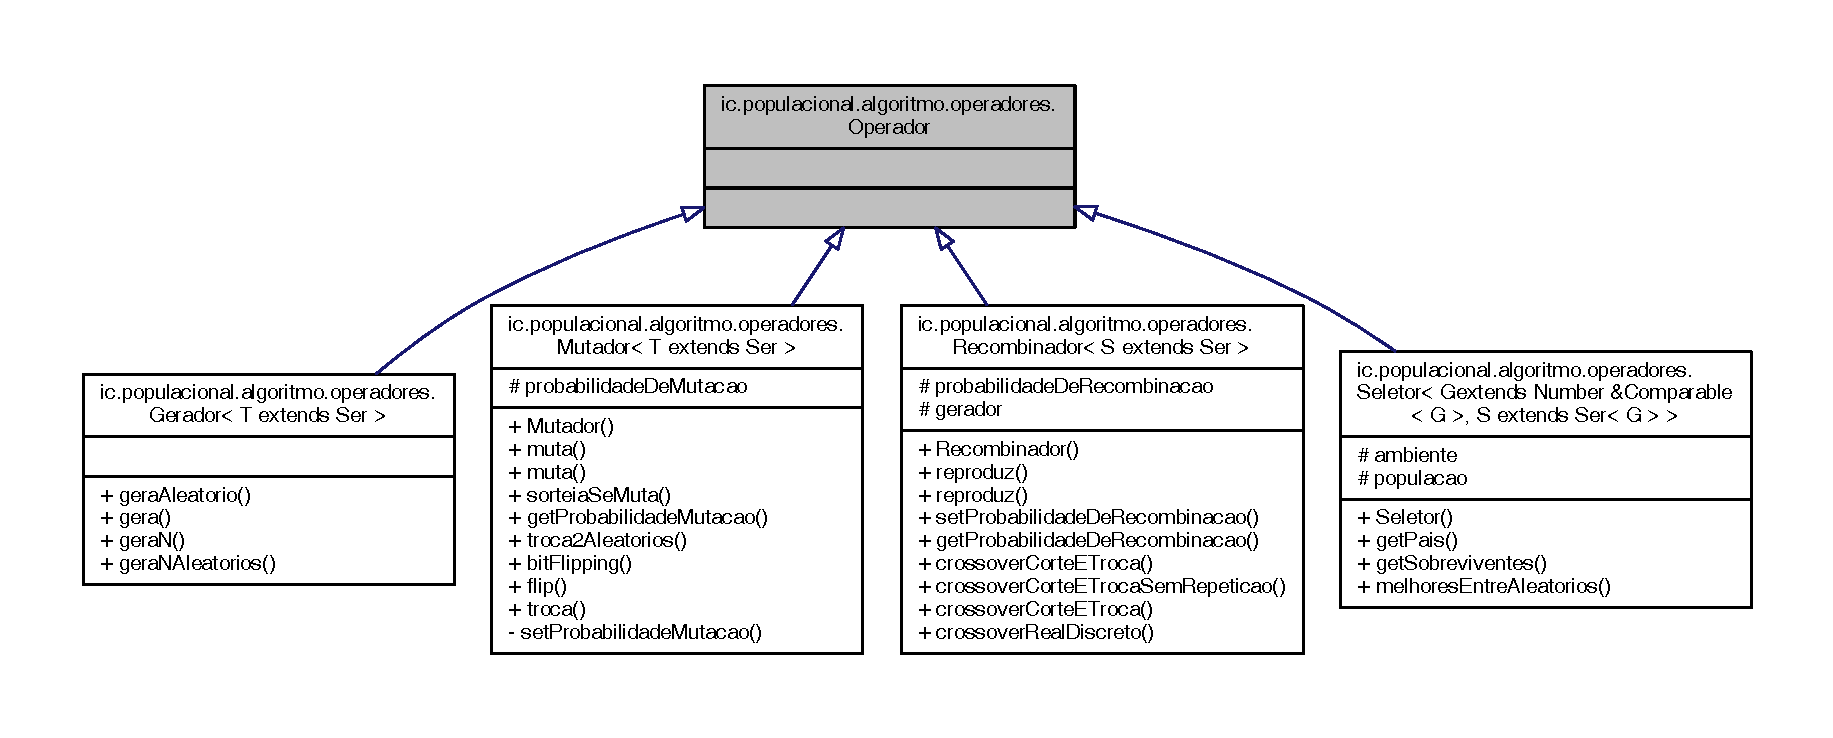
\includegraphics[width=350pt]{classic_1_1populacional_1_1algoritmo_1_1operadores_1_1_operador__inherit__graph}
\end{center}
\end{figure}


Diagrama de colaboração para ic.\-populacional.\-algoritmo.\-operadores.\-Operador\-:\nopagebreak
\begin{figure}[H]
\begin{center}
\leavevmode
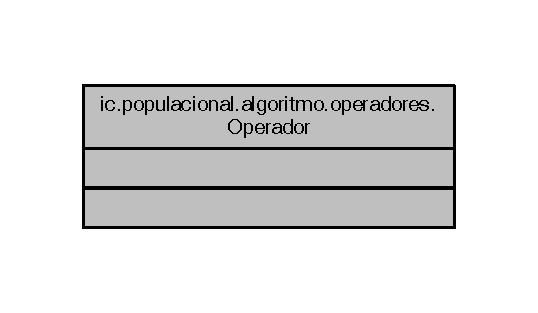
\includegraphics[width=258pt]{classic_1_1populacional_1_1algoritmo_1_1operadores_1_1_operador__coll__graph}
\end{center}
\end{figure}


\subsection{Descrição Detalhada}
\begin{DoxyAuthor}{Autor}
Victor de Lima Soares 
\end{DoxyAuthor}


A documentação para esta classe foi gerada a partir do seguinte arquivo\-:\begin{DoxyCompactItemize}
\item 
C\-:/\-Users/\-Victor/workplace/\-Net\-Beans\-Projects/\-Inteligencia Computacional/src/ic/populacional/algoritmo/operadores/\hyperlink{_operador_8java}{Operador.\-java}\end{DoxyCompactItemize}

\hypertarget{classic_1_1populacional_1_1algoritmo_1_1operadores_1_1recombinador_1_1_p_m_x_3_01_s_01extends_01_ser_01_4}{\section{Referência da Classe ic.\-populacional.\-algoritmo.\-operadores.\-recombinador.\-P\-M\-X$<$ S extends Ser $>$}
\label{classic_1_1populacional_1_1algoritmo_1_1operadores_1_1recombinador_1_1_p_m_x_3_01_s_01extends_01_ser_01_4}\index{ic.\-populacional.\-algoritmo.\-operadores.\-recombinador.\-P\-M\-X$<$ S extends Ser $>$@{ic.\-populacional.\-algoritmo.\-operadores.\-recombinador.\-P\-M\-X$<$ S extends Ser $>$}}
}


Partially Mapped Crossover (P\-X\-M).  




Diagrama de Hierarquia para ic.\-populacional.\-algoritmo.\-operadores.\-recombinador.\-P\-M\-X$<$ S extends Ser $>$\-:\nopagebreak
\begin{figure}[H]
\begin{center}
\leavevmode
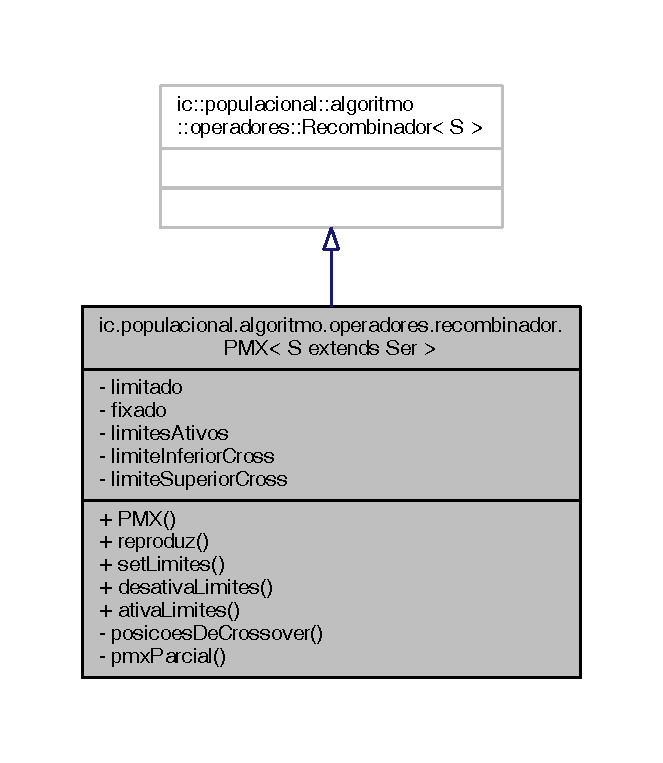
\includegraphics[width=318pt]{classic_1_1populacional_1_1algoritmo_1_1operadores_1_1recombinador_1_1_p_m_x_3_01_s_01extends_01_ser_01_4__inherit__graph}
\end{center}
\end{figure}


Diagrama de colaboração para ic.\-populacional.\-algoritmo.\-operadores.\-recombinador.\-P\-M\-X$<$ S extends Ser $>$\-:\nopagebreak
\begin{figure}[H]
\begin{center}
\leavevmode
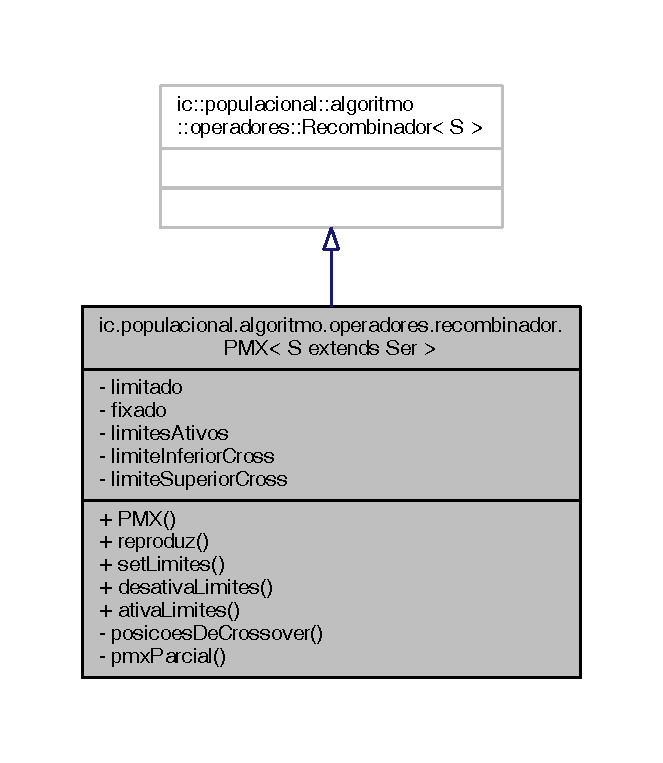
\includegraphics[width=318pt]{classic_1_1populacional_1_1algoritmo_1_1operadores_1_1recombinador_1_1_p_m_x_3_01_s_01extends_01_ser_01_4__coll__graph}
\end{center}
\end{figure}
\subsection*{Métodos Públicos}
\begin{DoxyCompactItemize}
\item 
\hyperlink{classic_1_1populacional_1_1algoritmo_1_1operadores_1_1recombinador_1_1_p_m_x_3_01_s_01extends_01_ser_01_4_ac4fad24a78c23a67d7073e52039c4424}{P\-M\-X} (Gerador$<$ S $>$ gerador, double probabilidade\-De\-Recombinacao)
\item 
List$<$ S $>$ \hyperlink{classic_1_1populacional_1_1algoritmo_1_1operadores_1_1recombinador_1_1_p_m_x_3_01_s_01extends_01_ser_01_4_a485bfc7d2615c87f8fbff6ae15092b89}{reproduz} (List$<$ S $>$ pares)
\item 
void \hyperlink{classic_1_1populacional_1_1algoritmo_1_1operadores_1_1recombinador_1_1_p_m_x_3_01_s_01extends_01_ser_01_4_aa8d1dcb410f1d9d49e4ab44b54f81c30}{set\-Limites} (int \hyperlink{classic_1_1populacional_1_1algoritmo_1_1operadores_1_1recombinador_1_1_p_m_x_3_01_s_01extends_01_ser_01_4_afa30d091104d7e520e3d1612a8453ee0}{limite\-Inferior\-Cross}, int \hyperlink{classic_1_1populacional_1_1algoritmo_1_1operadores_1_1recombinador_1_1_p_m_x_3_01_s_01extends_01_ser_01_4_ab3e6575836e6b19fa425076b30e90d70}{limite\-Superior\-Cross}, boolean fixa\-Posicoes)
\begin{DoxyCompactList}\small\item\em Atribui limites as posições de crossover, e os ativa. \end{DoxyCompactList}\item 
void \hyperlink{classic_1_1populacional_1_1algoritmo_1_1operadores_1_1recombinador_1_1_p_m_x_3_01_s_01extends_01_ser_01_4_a935e288b2dc08ad06437e92b96fcc0c9}{desativa\-Limites} ()
\begin{DoxyCompactList}\small\item\em Desativa, sem apagar, os limites impostos as posições de crossover. \end{DoxyCompactList}\item 
void \hyperlink{classic_1_1populacional_1_1algoritmo_1_1operadores_1_1recombinador_1_1_p_m_x_3_01_s_01extends_01_ser_01_4_a39c7f88521329ccd555468400d25d8b5}{ativa\-Limites} ()
\begin{DoxyCompactList}\small\item\em Ativa, os limites impostos as posições de crossover. \end{DoxyCompactList}\end{DoxyCompactItemize}
\subsection*{Métodos Privados}
\begin{DoxyCompactItemize}
\item 
List$<$ Integer $>$ \hyperlink{classic_1_1populacional_1_1algoritmo_1_1operadores_1_1recombinador_1_1_p_m_x_3_01_s_01extends_01_ser_01_4_ae728332ad4003249c953ea7e40fbc5f3}{posicoes\-De\-Crossover} (Ser par)
\begin{DoxyCompactList}\small\item\em Calcula as posições de crossover. \end{DoxyCompactList}\item 
S \hyperlink{classic_1_1populacional_1_1algoritmo_1_1operadores_1_1recombinador_1_1_p_m_x_3_01_s_01extends_01_ser_01_4_afd1da8537104869eca9569500487c041}{pmx\-Parcial} (S par1, S par2, int crossover1, int crossover2)
\begin{DoxyCompactList}\small\item\em Realiza cruzamento, gerando um filho. \end{DoxyCompactList}\end{DoxyCompactItemize}
\subsection*{Atributos Privados}
\begin{DoxyCompactItemize}
\item 
boolean \hyperlink{classic_1_1populacional_1_1algoritmo_1_1operadores_1_1recombinador_1_1_p_m_x_3_01_s_01extends_01_ser_01_4_abb460a5b5ce5c65297867a7284418498}{limitado} = false
\item 
boolean \hyperlink{classic_1_1populacional_1_1algoritmo_1_1operadores_1_1recombinador_1_1_p_m_x_3_01_s_01extends_01_ser_01_4_affd416ddea8d26b202849366ea345d2d}{fixado} = false
\item 
boolean \hyperlink{classic_1_1populacional_1_1algoritmo_1_1operadores_1_1recombinador_1_1_p_m_x_3_01_s_01extends_01_ser_01_4_a92c5e45dcd2dc819f0184277d563e018}{limites\-Ativos} = false
\item 
int \hyperlink{classic_1_1populacional_1_1algoritmo_1_1operadores_1_1recombinador_1_1_p_m_x_3_01_s_01extends_01_ser_01_4_afa30d091104d7e520e3d1612a8453ee0}{limite\-Inferior\-Cross}
\item 
int \hyperlink{classic_1_1populacional_1_1algoritmo_1_1operadores_1_1recombinador_1_1_p_m_x_3_01_s_01extends_01_ser_01_4_ab3e6575836e6b19fa425076b30e90d70}{limite\-Superior\-Cross}
\end{DoxyCompactItemize}


\subsection{Descrição Detalhada}
Partially Mapped Crossover (P\-X\-M). 

Recombinação para representações baseadas em permutações. 

\paragraph*{Passos\-:}


\begin{DoxyEnumerate}
\item Escolhe dois pontos de crossover aleatoriamente; 
\item Copia todos os elementos de P1 entre os pontos no filho, nas mesmas posições ocupadas em P1; 
\item Para cada elemento entre os pontos de crossover em P2 ainda não adicionado, adiciona-\/o ao filho, na posição ocupada pelo ponto proveniente de P1 em P2\-: 
\begin{DoxyItemize}
\item Para o elemento na posição {\itshape i} em P2, busca no filho o elemento que ocupa a mesma posição {\itshape i}, de valor {\itshape n};  
\item A posição do elemento com valor {\itshape n} será então {\itshape j}, definido pela posição {\itshape j} em P2, cujo valor também seja {\itshape n};  
\item Em caso de conflito, quando {\itshape j} indica uma posição já ocupada, repete-\/se o processo até que uma posição vazia seja encontrada.  
\end{DoxyItemize}
\item Copia-\/se o restante dos elementos provenientes de P2; 
\item Realiza-\/se o mesmo procedimento para a obtenção de um segundo filho, invertendo os papeis de P1 e P2. 
\end{DoxyEnumerate}

\begin{DoxyAuthor}{Autor}
Victor de Lima Soares 
\end{DoxyAuthor}
\begin{DoxyVersion}{Versão}
1.\-0
\end{DoxyVersion}

\begin{DoxyParams}{Parâmetros}
{\em $<$\-S$>$} & Classe dos Seres. \\
\hline
\end{DoxyParams}


\subsection{Construtores \& Destrutores}
\hypertarget{classic_1_1populacional_1_1algoritmo_1_1operadores_1_1recombinador_1_1_p_m_x_3_01_s_01extends_01_ser_01_4_ac4fad24a78c23a67d7073e52039c4424}{\index{ic\-::populacional\-::algoritmo\-::operadores\-::recombinador\-::\-P\-M\-X$<$ S extends Ser $>$@{ic\-::populacional\-::algoritmo\-::operadores\-::recombinador\-::\-P\-M\-X$<$ S extends Ser $>$}!P\-M\-X@{P\-M\-X}}
\index{P\-M\-X@{P\-M\-X}!ic::populacional::algoritmo::operadores::recombinador::PMX< S extends Ser >@{ic\-::populacional\-::algoritmo\-::operadores\-::recombinador\-::\-P\-M\-X$<$ S extends Ser $>$}}
\subsubsection[{P\-M\-X}]{\setlength{\rightskip}{0pt plus 5cm}ic.\-populacional.\-algoritmo.\-operadores.\-recombinador.\-P\-M\-X$<$ S extends Ser $>$.P\-M\-X (
\begin{DoxyParamCaption}
\item[{Gerador$<$ S $>$}]{gerador, }
\item[{double}]{probabilidade\-De\-Recombinacao}
\end{DoxyParamCaption}
)}}\label{classic_1_1populacional_1_1algoritmo_1_1operadores_1_1recombinador_1_1_p_m_x_3_01_s_01extends_01_ser_01_4_ac4fad24a78c23a67d7073e52039c4424}


\subsection{Métodos}
\hypertarget{classic_1_1populacional_1_1algoritmo_1_1operadores_1_1recombinador_1_1_p_m_x_3_01_s_01extends_01_ser_01_4_a39c7f88521329ccd555468400d25d8b5}{\index{ic\-::populacional\-::algoritmo\-::operadores\-::recombinador\-::\-P\-M\-X$<$ S extends Ser $>$@{ic\-::populacional\-::algoritmo\-::operadores\-::recombinador\-::\-P\-M\-X$<$ S extends Ser $>$}!ativa\-Limites@{ativa\-Limites}}
\index{ativa\-Limites@{ativa\-Limites}!ic::populacional::algoritmo::operadores::recombinador::PMX< S extends Ser >@{ic\-::populacional\-::algoritmo\-::operadores\-::recombinador\-::\-P\-M\-X$<$ S extends Ser $>$}}
\subsubsection[{ativa\-Limites}]{\setlength{\rightskip}{0pt plus 5cm}void ic.\-populacional.\-algoritmo.\-operadores.\-recombinador.\-P\-M\-X$<$ S extends Ser $>$.ativa\-Limites (
\begin{DoxyParamCaption}
{}
\end{DoxyParamCaption}
)}}\label{classic_1_1populacional_1_1algoritmo_1_1operadores_1_1recombinador_1_1_p_m_x_3_01_s_01extends_01_ser_01_4_a39c7f88521329ccd555468400d25d8b5}


Ativa, os limites impostos as posições de crossover. 

\begin{DoxySince}{Desde}
1.\-0
\end{DoxySince}

\begin{DoxyExceptions}{Exceções}
{\em Illegal\-State\-Exception} & Se 
\begin{DoxyItemize}
\item 
\end{DoxyItemize}não estiverem sido atribuídos.  \\
\hline
\end{DoxyExceptions}
\hypertarget{classic_1_1populacional_1_1algoritmo_1_1operadores_1_1recombinador_1_1_p_m_x_3_01_s_01extends_01_ser_01_4_a935e288b2dc08ad06437e92b96fcc0c9}{\index{ic\-::populacional\-::algoritmo\-::operadores\-::recombinador\-::\-P\-M\-X$<$ S extends Ser $>$@{ic\-::populacional\-::algoritmo\-::operadores\-::recombinador\-::\-P\-M\-X$<$ S extends Ser $>$}!desativa\-Limites@{desativa\-Limites}}
\index{desativa\-Limites@{desativa\-Limites}!ic::populacional::algoritmo::operadores::recombinador::PMX< S extends Ser >@{ic\-::populacional\-::algoritmo\-::operadores\-::recombinador\-::\-P\-M\-X$<$ S extends Ser $>$}}
\subsubsection[{desativa\-Limites}]{\setlength{\rightskip}{0pt plus 5cm}void ic.\-populacional.\-algoritmo.\-operadores.\-recombinador.\-P\-M\-X$<$ S extends Ser $>$.desativa\-Limites (
\begin{DoxyParamCaption}
{}
\end{DoxyParamCaption}
)}}\label{classic_1_1populacional_1_1algoritmo_1_1operadores_1_1recombinador_1_1_p_m_x_3_01_s_01extends_01_ser_01_4_a935e288b2dc08ad06437e92b96fcc0c9}


Desativa, sem apagar, os limites impostos as posições de crossover. 

\begin{DoxySince}{Desde}
1.\-0 
\end{DoxySince}
\hypertarget{classic_1_1populacional_1_1algoritmo_1_1operadores_1_1recombinador_1_1_p_m_x_3_01_s_01extends_01_ser_01_4_afd1da8537104869eca9569500487c041}{\index{ic\-::populacional\-::algoritmo\-::operadores\-::recombinador\-::\-P\-M\-X$<$ S extends Ser $>$@{ic\-::populacional\-::algoritmo\-::operadores\-::recombinador\-::\-P\-M\-X$<$ S extends Ser $>$}!pmx\-Parcial@{pmx\-Parcial}}
\index{pmx\-Parcial@{pmx\-Parcial}!ic::populacional::algoritmo::operadores::recombinador::PMX< S extends Ser >@{ic\-::populacional\-::algoritmo\-::operadores\-::recombinador\-::\-P\-M\-X$<$ S extends Ser $>$}}
\subsubsection[{pmx\-Parcial}]{\setlength{\rightskip}{0pt plus 5cm}S ic.\-populacional.\-algoritmo.\-operadores.\-recombinador.\-P\-M\-X$<$ S extends Ser $>$.pmx\-Parcial (
\begin{DoxyParamCaption}
\item[{S}]{par1, }
\item[{S}]{par2, }
\item[{int}]{crossover1, }
\item[{int}]{crossover2}
\end{DoxyParamCaption}
)\hspace{0.3cm}{\ttfamily [private]}}}\label{classic_1_1populacional_1_1algoritmo_1_1operadores_1_1recombinador_1_1_p_m_x_3_01_s_01extends_01_ser_01_4_afd1da8537104869eca9569500487c041}


Realiza cruzamento, gerando um filho. 

\paragraph*{Passos\-:}


\begin{DoxyEnumerate}
\item Escolhe dois pontos de crossover aleatoriamente; 
\item Copia todos os elementos de P1 entre os pontos no filho, nas mesmas posições ocupadas em P1; 
\item Para cada elemento entre os pontos de crossover em P2 ainda não adicionado, adiciona-\/o ao filho, na posição ocupada pelo ponto proveniente de P1 em P2\-: 
\begin{DoxyItemize}
\item Para o elemento na posição {\itshape i} em P2, busca no filho o elemento que ocupa a mesma posição {\itshape i}, de valor {\itshape n};  
\item A posição do elemento com valor {\itshape n} será então {\itshape j}, definido pela posição {\itshape j} em P2, cujo valor também seja {\itshape n};  
\item Em caso de conflito, quando {\itshape j} indica uma posição já ocupada, repete-\/se o processo até que uma posição vazia seja encontrada.  
\end{DoxyItemize}
\item Copia-\/se o restante dos elementos provenientes de P2. 
\end{DoxyEnumerate}

{\bfseries A ordem dos progenitores altera o resultado.}


\begin{DoxyParams}{Parâmetros}
{\em par1} & Primeiro progenitor. \\
\hline
{\em par2} & Segundo progenitor. \\
\hline
{\em crossover1} & Posição de corte\-: posição inicial. \\
\hline
{\em crossover2} & Posição de corte\-: posição final. \\
\hline
\end{DoxyParams}
\begin{DoxyReturn}{Retorna}
filho gerado. 
\end{DoxyReturn}
\hypertarget{classic_1_1populacional_1_1algoritmo_1_1operadores_1_1recombinador_1_1_p_m_x_3_01_s_01extends_01_ser_01_4_ae728332ad4003249c953ea7e40fbc5f3}{\index{ic\-::populacional\-::algoritmo\-::operadores\-::recombinador\-::\-P\-M\-X$<$ S extends Ser $>$@{ic\-::populacional\-::algoritmo\-::operadores\-::recombinador\-::\-P\-M\-X$<$ S extends Ser $>$}!posicoes\-De\-Crossover@{posicoes\-De\-Crossover}}
\index{posicoes\-De\-Crossover@{posicoes\-De\-Crossover}!ic::populacional::algoritmo::operadores::recombinador::PMX< S extends Ser >@{ic\-::populacional\-::algoritmo\-::operadores\-::recombinador\-::\-P\-M\-X$<$ S extends Ser $>$}}
\subsubsection[{posicoes\-De\-Crossover}]{\setlength{\rightskip}{0pt plus 5cm}List$<$Integer$>$ ic.\-populacional.\-algoritmo.\-operadores.\-recombinador.\-P\-M\-X$<$ S extends Ser $>$.posicoes\-De\-Crossover (
\begin{DoxyParamCaption}
\item[{Ser}]{par}
\end{DoxyParamCaption}
)\hspace{0.3cm}{\ttfamily [private]}}}\label{classic_1_1populacional_1_1algoritmo_1_1operadores_1_1recombinador_1_1_p_m_x_3_01_s_01extends_01_ser_01_4_ae728332ad4003249c953ea7e40fbc5f3}


Calcula as posições de crossover. 

\begin{DoxySince}{Desde}
1.\-0 
\end{DoxySince}

\begin{DoxyParams}{Parâmetros}
{\em par} & Ser base para cálculo dos índices\-: usado apenas para delimitar os limites de tamanho. \\
\hline
\end{DoxyParams}
\begin{DoxyReturn}{Retorna}
Lista com as posições de crossover. 
\end{DoxyReturn}
\hypertarget{classic_1_1populacional_1_1algoritmo_1_1operadores_1_1recombinador_1_1_p_m_x_3_01_s_01extends_01_ser_01_4_a485bfc7d2615c87f8fbff6ae15092b89}{\index{ic\-::populacional\-::algoritmo\-::operadores\-::recombinador\-::\-P\-M\-X$<$ S extends Ser $>$@{ic\-::populacional\-::algoritmo\-::operadores\-::recombinador\-::\-P\-M\-X$<$ S extends Ser $>$}!reproduz@{reproduz}}
\index{reproduz@{reproduz}!ic::populacional::algoritmo::operadores::recombinador::PMX< S extends Ser >@{ic\-::populacional\-::algoritmo\-::operadores\-::recombinador\-::\-P\-M\-X$<$ S extends Ser $>$}}
\subsubsection[{reproduz}]{\setlength{\rightskip}{0pt plus 5cm}List$<$S$>$ ic.\-populacional.\-algoritmo.\-operadores.\-recombinador.\-P\-M\-X$<$ S extends Ser $>$.reproduz (
\begin{DoxyParamCaption}
\item[{List$<$ S $>$}]{pares}
\end{DoxyParamCaption}
)}}\label{classic_1_1populacional_1_1algoritmo_1_1operadores_1_1recombinador_1_1_p_m_x_3_01_s_01extends_01_ser_01_4_a485bfc7d2615c87f8fbff6ae15092b89}
\begin{DoxySince}{Desde}
1.\-0 
\end{DoxySince}
\hypertarget{classic_1_1populacional_1_1algoritmo_1_1operadores_1_1recombinador_1_1_p_m_x_3_01_s_01extends_01_ser_01_4_aa8d1dcb410f1d9d49e4ab44b54f81c30}{\index{ic\-::populacional\-::algoritmo\-::operadores\-::recombinador\-::\-P\-M\-X$<$ S extends Ser $>$@{ic\-::populacional\-::algoritmo\-::operadores\-::recombinador\-::\-P\-M\-X$<$ S extends Ser $>$}!set\-Limites@{set\-Limites}}
\index{set\-Limites@{set\-Limites}!ic::populacional::algoritmo::operadores::recombinador::PMX< S extends Ser >@{ic\-::populacional\-::algoritmo\-::operadores\-::recombinador\-::\-P\-M\-X$<$ S extends Ser $>$}}
\subsubsection[{set\-Limites}]{\setlength{\rightskip}{0pt plus 5cm}void ic.\-populacional.\-algoritmo.\-operadores.\-recombinador.\-P\-M\-X$<$ S extends Ser $>$.set\-Limites (
\begin{DoxyParamCaption}
\item[{int}]{limite\-Inferior\-Cross, }
\item[{int}]{limite\-Superior\-Cross, }
\item[{boolean}]{fixa\-Posicoes}
\end{DoxyParamCaption}
)}}\label{classic_1_1populacional_1_1algoritmo_1_1operadores_1_1recombinador_1_1_p_m_x_3_01_s_01extends_01_ser_01_4_aa8d1dcb410f1d9d49e4ab44b54f81c30}


Atribui limites as posições de crossover, e os ativa. 

\begin{DoxySince}{Desde}
1.\-0 
\end{DoxySince}

\begin{DoxyParams}{Parâmetros}
{\em limite\-Inferior\-Cross} & Limite inferior, maior que zero. \\
\hline
{\em limite\-Superior\-Cross} & Limite superior, maior que zero. \\
\hline
{\em fixa\-Posicoes} & Define se as posições de corte devem ser aleatórias ou fixadas nos limites.\\
\hline
\end{DoxyParams}

\begin{DoxyExceptions}{Exceções}
{\em Illegal\-Argument\-Exception} & Se 
\begin{DoxyItemize}
\item Limite inferior for menor que zero;  
\item Limite superior for menor que o limite inferior;  
\end{DoxyItemize}\\
\hline
\end{DoxyExceptions}


\subsection{Atributos}
\hypertarget{classic_1_1populacional_1_1algoritmo_1_1operadores_1_1recombinador_1_1_p_m_x_3_01_s_01extends_01_ser_01_4_affd416ddea8d26b202849366ea345d2d}{\index{ic\-::populacional\-::algoritmo\-::operadores\-::recombinador\-::\-P\-M\-X$<$ S extends Ser $>$@{ic\-::populacional\-::algoritmo\-::operadores\-::recombinador\-::\-P\-M\-X$<$ S extends Ser $>$}!fixado@{fixado}}
\index{fixado@{fixado}!ic::populacional::algoritmo::operadores::recombinador::PMX< S extends Ser >@{ic\-::populacional\-::algoritmo\-::operadores\-::recombinador\-::\-P\-M\-X$<$ S extends Ser $>$}}
\subsubsection[{fixado}]{\setlength{\rightskip}{0pt plus 5cm}boolean ic.\-populacional.\-algoritmo.\-operadores.\-recombinador.\-P\-M\-X$<$ S extends Ser $>$.fixado = false\hspace{0.3cm}{\ttfamily [private]}}}\label{classic_1_1populacional_1_1algoritmo_1_1operadores_1_1recombinador_1_1_p_m_x_3_01_s_01extends_01_ser_01_4_affd416ddea8d26b202849366ea345d2d}
\hypertarget{classic_1_1populacional_1_1algoritmo_1_1operadores_1_1recombinador_1_1_p_m_x_3_01_s_01extends_01_ser_01_4_abb460a5b5ce5c65297867a7284418498}{\index{ic\-::populacional\-::algoritmo\-::operadores\-::recombinador\-::\-P\-M\-X$<$ S extends Ser $>$@{ic\-::populacional\-::algoritmo\-::operadores\-::recombinador\-::\-P\-M\-X$<$ S extends Ser $>$}!limitado@{limitado}}
\index{limitado@{limitado}!ic::populacional::algoritmo::operadores::recombinador::PMX< S extends Ser >@{ic\-::populacional\-::algoritmo\-::operadores\-::recombinador\-::\-P\-M\-X$<$ S extends Ser $>$}}
\subsubsection[{limitado}]{\setlength{\rightskip}{0pt plus 5cm}boolean ic.\-populacional.\-algoritmo.\-operadores.\-recombinador.\-P\-M\-X$<$ S extends Ser $>$.limitado = false\hspace{0.3cm}{\ttfamily [private]}}}\label{classic_1_1populacional_1_1algoritmo_1_1operadores_1_1recombinador_1_1_p_m_x_3_01_s_01extends_01_ser_01_4_abb460a5b5ce5c65297867a7284418498}
\hypertarget{classic_1_1populacional_1_1algoritmo_1_1operadores_1_1recombinador_1_1_p_m_x_3_01_s_01extends_01_ser_01_4_afa30d091104d7e520e3d1612a8453ee0}{\index{ic\-::populacional\-::algoritmo\-::operadores\-::recombinador\-::\-P\-M\-X$<$ S extends Ser $>$@{ic\-::populacional\-::algoritmo\-::operadores\-::recombinador\-::\-P\-M\-X$<$ S extends Ser $>$}!limite\-Inferior\-Cross@{limite\-Inferior\-Cross}}
\index{limite\-Inferior\-Cross@{limite\-Inferior\-Cross}!ic::populacional::algoritmo::operadores::recombinador::PMX< S extends Ser >@{ic\-::populacional\-::algoritmo\-::operadores\-::recombinador\-::\-P\-M\-X$<$ S extends Ser $>$}}
\subsubsection[{limite\-Inferior\-Cross}]{\setlength{\rightskip}{0pt plus 5cm}int ic.\-populacional.\-algoritmo.\-operadores.\-recombinador.\-P\-M\-X$<$ S extends Ser $>$.limite\-Inferior\-Cross\hspace{0.3cm}{\ttfamily [private]}}}\label{classic_1_1populacional_1_1algoritmo_1_1operadores_1_1recombinador_1_1_p_m_x_3_01_s_01extends_01_ser_01_4_afa30d091104d7e520e3d1612a8453ee0}
\hypertarget{classic_1_1populacional_1_1algoritmo_1_1operadores_1_1recombinador_1_1_p_m_x_3_01_s_01extends_01_ser_01_4_a92c5e45dcd2dc819f0184277d563e018}{\index{ic\-::populacional\-::algoritmo\-::operadores\-::recombinador\-::\-P\-M\-X$<$ S extends Ser $>$@{ic\-::populacional\-::algoritmo\-::operadores\-::recombinador\-::\-P\-M\-X$<$ S extends Ser $>$}!limites\-Ativos@{limites\-Ativos}}
\index{limites\-Ativos@{limites\-Ativos}!ic::populacional::algoritmo::operadores::recombinador::PMX< S extends Ser >@{ic\-::populacional\-::algoritmo\-::operadores\-::recombinador\-::\-P\-M\-X$<$ S extends Ser $>$}}
\subsubsection[{limites\-Ativos}]{\setlength{\rightskip}{0pt plus 5cm}boolean ic.\-populacional.\-algoritmo.\-operadores.\-recombinador.\-P\-M\-X$<$ S extends Ser $>$.limites\-Ativos = false\hspace{0.3cm}{\ttfamily [private]}}}\label{classic_1_1populacional_1_1algoritmo_1_1operadores_1_1recombinador_1_1_p_m_x_3_01_s_01extends_01_ser_01_4_a92c5e45dcd2dc819f0184277d563e018}
\hypertarget{classic_1_1populacional_1_1algoritmo_1_1operadores_1_1recombinador_1_1_p_m_x_3_01_s_01extends_01_ser_01_4_ab3e6575836e6b19fa425076b30e90d70}{\index{ic\-::populacional\-::algoritmo\-::operadores\-::recombinador\-::\-P\-M\-X$<$ S extends Ser $>$@{ic\-::populacional\-::algoritmo\-::operadores\-::recombinador\-::\-P\-M\-X$<$ S extends Ser $>$}!limite\-Superior\-Cross@{limite\-Superior\-Cross}}
\index{limite\-Superior\-Cross@{limite\-Superior\-Cross}!ic::populacional::algoritmo::operadores::recombinador::PMX< S extends Ser >@{ic\-::populacional\-::algoritmo\-::operadores\-::recombinador\-::\-P\-M\-X$<$ S extends Ser $>$}}
\subsubsection[{limite\-Superior\-Cross}]{\setlength{\rightskip}{0pt plus 5cm}int ic.\-populacional.\-algoritmo.\-operadores.\-recombinador.\-P\-M\-X$<$ S extends Ser $>$.limite\-Superior\-Cross\hspace{0.3cm}{\ttfamily [private]}}}\label{classic_1_1populacional_1_1algoritmo_1_1operadores_1_1recombinador_1_1_p_m_x_3_01_s_01extends_01_ser_01_4_ab3e6575836e6b19fa425076b30e90d70}


A documentação para esta classe foi gerada a partir do seguinte arquivo\-:\begin{DoxyCompactItemize}
\item 
C\-:/\-Users/\-Victor/workplace/\-Net\-Beans\-Projects/\-Inteligencia Computacional/src/ic/populacional/algoritmo/operadores/recombinador/\hyperlink{_p_m_x_8java}{P\-M\-X.\-java}\end{DoxyCompactItemize}

\hypertarget{classic_1_1populacional_1_1_populacao_3_01_g_01extends_01_number_01_6_comparable_3_01_g_01_4_00_506237fa66af7bbd01f529b68d4beaca}{\section{Referência da Classe ic.\-populacional.\-Populacao$<$ G extends Number \&Comparable$<$ G $>$, S extends Ser$<$ G $>$ $>$}
\label{classic_1_1populacional_1_1_populacao_3_01_g_01extends_01_number_01_6_comparable_3_01_g_01_4_00_506237fa66af7bbd01f529b68d4beaca}\index{ic.\-populacional.\-Populacao$<$ G extends Number \&\-Comparable$<$ G $>$, S extends Ser$<$ G $>$ $>$@{ic.\-populacional.\-Populacao$<$ G extends Number \&\-Comparable$<$ G $>$, S extends Ser$<$ G $>$ $>$}}
}


Abstração do conceito\-: “população”; conjunto de seres.  




Diagrama de Hierarquia para ic.\-populacional.\-Populacao$<$ G extends Number \&Comparable$<$ G $>$, S extends Ser$<$ G $>$ $>$\-:
\nopagebreak
\begin{figure}[H]
\begin{center}
\leavevmode
\includegraphics[width=248pt]{classic_1_1populacional_1_1_populacao_3_01_g_01extends_01_number_01_6_comparable_3_01_g_01_4_00_fe344a962d2d07afef79097d39aa7a37}
\end{center}
\end{figure}


Diagrama de colaboração para ic.\-populacional.\-Populacao$<$ G extends Number \&Comparable$<$ G $>$, S extends Ser$<$ G $>$ $>$\-:
\nopagebreak
\begin{figure}[H]
\begin{center}
\leavevmode
\includegraphics[width=350pt]{classic_1_1populacional_1_1_populacao_3_01_g_01extends_01_number_01_6_comparable_3_01_g_01_4_00_599b14e6302ec6435a84d6a33405323f}
\end{center}
\end{figure}
\subsection*{Métodos Públicos}
\begin{DoxyCompactItemize}
\item 
\hyperlink{classic_1_1populacional_1_1_populacao_3_01_g_01extends_01_number_01_6_comparable_3_01_g_01_4_00_506237fa66af7bbd01f529b68d4beaca_ac36f770357cb6c012dce49439b303034}{Populacao} (Ambiente$<$ G, S $>$ \hyperlink{classic_1_1populacional_1_1_populacao_3_01_g_01extends_01_number_01_6_comparable_3_01_g_01_4_00_506237fa66af7bbd01f529b68d4beaca_a12c7cdc6e608deccb84e397ec9dd43dc}{ambiente}, int \hyperlink{classic_1_1populacional_1_1_populacao_3_01_g_01extends_01_number_01_6_comparable_3_01_g_01_4_00_506237fa66af7bbd01f529b68d4beaca_afcdf79ace747a488138db50b05fb21b0}{max\-Individuos})
\begin{DoxyCompactList}\small\item\em Construtor. \end{DoxyCompactList}\item 
boolean \hyperlink{classic_1_1populacional_1_1_populacao_3_01_g_01extends_01_number_01_6_comparable_3_01_g_01_4_00_506237fa66af7bbd01f529b68d4beaca_a1dbf6d55d4479aa588fb085997190cc8}{set\-Individuos} (Collection$<$?extends S $>$ \hyperlink{classic_1_1populacional_1_1_populacao_3_01_g_01extends_01_number_01_6_comparable_3_01_g_01_4_00_506237fa66af7bbd01f529b68d4beaca_a95b7dbe0db4e648740672366ee01877f}{seres})
\begin{DoxyCompactList}\small\item\em Esvazia a população e adiciona a ela a coleção passada como parâmetro. \end{DoxyCompactList}\item 
boolean \hyperlink{classic_1_1populacional_1_1_populacao_3_01_g_01extends_01_number_01_6_comparable_3_01_g_01_4_00_506237fa66af7bbd01f529b68d4beaca_af252d7151066b5cf0b044c63c5ad2a34}{add\-All} (Collection$<$?extends S $>$ \hyperlink{classic_1_1populacional_1_1_populacao_3_01_g_01extends_01_number_01_6_comparable_3_01_g_01_4_00_506237fa66af7bbd01f529b68d4beaca_a95b7dbe0db4e648740672366ee01877f}{seres})
\begin{DoxyCompactList}\small\item\em Adiciona uma coleção de seres a população. \end{DoxyCompactList}\item 
boolean \hyperlink{classic_1_1populacional_1_1_populacao_3_01_g_01extends_01_number_01_6_comparable_3_01_g_01_4_00_506237fa66af7bbd01f529b68d4beaca_af3202776ab8e02e8f0f15a2e7ef3a2bd}{add} (S ser)
\begin{DoxyCompactList}\small\item\em Adiciona um ser a população. \end{DoxyCompactList}\item 
int \hyperlink{classic_1_1populacional_1_1_populacao_3_01_g_01extends_01_number_01_6_comparable_3_01_g_01_4_00_506237fa66af7bbd01f529b68d4beaca_a3c5abfad17ad8ea60283da169c385315}{get\-Max\-Individuos} ()
\begin{DoxyCompactList}\small\item\em Retorna o número máximo de seres nessa população. \end{DoxyCompactList}\item 
S \hyperlink{classic_1_1populacional_1_1_populacao_3_01_g_01extends_01_number_01_6_comparable_3_01_g_01_4_00_506237fa66af7bbd01f529b68d4beaca_acbcdb216574082cb970be119c590200d}{get} (int indice)
\begin{DoxyCompactList}\small\item\em Método para acessos baseado em índices. \end{DoxyCompactList}\item 
int \hyperlink{classic_1_1populacional_1_1_populacao_3_01_g_01extends_01_number_01_6_comparable_3_01_g_01_4_00_506237fa66af7bbd01f529b68d4beaca_a39f905ac398bd8ea00b8babb6d16c43a}{size} ()
\begin{DoxyCompactList}\small\item\em Retorna o número de seres na população. \end{DoxyCompactList}\item 
abstract S \hyperlink{classic_1_1populacional_1_1_populacao_3_01_g_01extends_01_number_01_6_comparable_3_01_g_01_4_00_506237fa66af7bbd01f529b68d4beaca_a1bbf2653a1ed8b5e5c1af9333767a033}{get\-Melhor} ()
\begin{DoxyCompactList}\small\item\em Retorna o ser mais adaptado da população. \end{DoxyCompactList}\item 
G \hyperlink{classic_1_1populacional_1_1_populacao_3_01_g_01extends_01_number_01_6_comparable_3_01_g_01_4_00_506237fa66af7bbd01f529b68d4beaca_a4ec654326f5d9a6cfec73dd55d4bd6b0}{get\-Melhor\-Grau} ()
\begin{DoxyCompactList}\small\item\em Retorna o grau de adaptação do ser mais adaptado na população. \end{DoxyCompactList}\item 
abstract List$<$ S $>$ \hyperlink{classic_1_1populacional_1_1_populacao_3_01_g_01extends_01_number_01_6_comparable_3_01_g_01_4_00_506237fa66af7bbd01f529b68d4beaca_acedbe86a5230401a6a6563af55ac94a0}{get\-N\-Melhores} (int n)
\begin{DoxyCompactList}\small\item\em Cria uma lista com os {\itshape n} melhores seres. \end{DoxyCompactList}\item 
boolean \hyperlink{classic_1_1populacional_1_1_populacao_3_01_g_01extends_01_number_01_6_comparable_3_01_g_01_4_00_506237fa66af7bbd01f529b68d4beaca_a1d96da8d70618b6af6bff59c1c5732d7}{is\-Empty} ()
\begin{DoxyCompactList}\small\item\em Verifica se a população está vazia. \end{DoxyCompactList}\item 
boolean \hyperlink{classic_1_1populacional_1_1_populacao_3_01_g_01extends_01_number_01_6_comparable_3_01_g_01_4_00_506237fa66af7bbd01f529b68d4beaca_aad5741e72c7f13742773db65e4632a6e}{contains} (Object ser)
\begin{DoxyCompactList}\small\item\em Verifica se o ser existe na população. \end{DoxyCompactList}\item 
boolean \hyperlink{classic_1_1populacional_1_1_populacao_3_01_g_01extends_01_number_01_6_comparable_3_01_g_01_4_00_506237fa66af7bbd01f529b68d4beaca_ab818a8582b19b47f32efce1943e2ddae}{contains\-All} (Collection$<$?$>$ \hyperlink{classic_1_1populacional_1_1_populacao_3_01_g_01extends_01_number_01_6_comparable_3_01_g_01_4_00_506237fa66af7bbd01f529b68d4beaca_a95b7dbe0db4e648740672366ee01877f}{seres})
\begin{DoxyCompactList}\small\item\em Verifica a existência de todos os elementos na coleção parâmetro. \end{DoxyCompactList}\item 
boolean \hyperlink{classic_1_1populacional_1_1_populacao_3_01_g_01extends_01_number_01_6_comparable_3_01_g_01_4_00_506237fa66af7bbd01f529b68d4beaca_ac71cb30ee867b21a7540e78547933b4b}{remove} (Object ser)
\begin{DoxyCompactList}\small\item\em Remove um elemento igual ao parâmetro da população. \end{DoxyCompactList}\item 
boolean \hyperlink{classic_1_1populacional_1_1_populacao_3_01_g_01extends_01_number_01_6_comparable_3_01_g_01_4_00_506237fa66af7bbd01f529b68d4beaca_a9d611c9b711c8cd04b2324efd551990e}{remove\-All} (Collection$<$?$>$ \hyperlink{classic_1_1populacional_1_1_populacao_3_01_g_01extends_01_number_01_6_comparable_3_01_g_01_4_00_506237fa66af7bbd01f529b68d4beaca_a95b7dbe0db4e648740672366ee01877f}{seres})
\begin{DoxyCompactList}\small\item\em Remove todos elementos iguais a algum elemento na coleção parâmetro. \end{DoxyCompactList}\item 
boolean \hyperlink{classic_1_1populacional_1_1_populacao_3_01_g_01extends_01_number_01_6_comparable_3_01_g_01_4_00_506237fa66af7bbd01f529b68d4beaca_ad25c10c70bddd4de2b54080903346a9b}{retain\-All} (Collection$<$?$>$ \hyperlink{classic_1_1populacional_1_1_populacao_3_01_g_01extends_01_number_01_6_comparable_3_01_g_01_4_00_506237fa66af7bbd01f529b68d4beaca_a95b7dbe0db4e648740672366ee01877f}{seres})
\begin{DoxyCompactList}\small\item\em Remove da população todos os elementos não pertencentes a coleção parâmetro. \end{DoxyCompactList}\item 
void \hyperlink{classic_1_1populacional_1_1_populacao_3_01_g_01extends_01_number_01_6_comparable_3_01_g_01_4_00_506237fa66af7bbd01f529b68d4beaca_a13c723f86e08b836040c27250e9468ee}{clear} ()
\begin{DoxyCompactList}\small\item\em Exclui todos os seres da população. \end{DoxyCompactList}\item 
Iterator$<$ S $>$ \hyperlink{classic_1_1populacional_1_1_populacao_3_01_g_01extends_01_number_01_6_comparable_3_01_g_01_4_00_506237fa66af7bbd01f529b68d4beaca_af42ba15859ae243a0692a55c8eae6df6}{iterator} ()
\begin{DoxyCompactList}\small\item\em Retorna um iterator para os seres na população. \end{DoxyCompactList}\item 
S\mbox{[}$\,$\mbox{]} \hyperlink{classic_1_1populacional_1_1_populacao_3_01_g_01extends_01_number_01_6_comparable_3_01_g_01_4_00_506237fa66af7bbd01f529b68d4beaca_af1b34b37800fbc016dc9b6ac9027213b}{to\-Array} ()
\begin{DoxyCompactList}\small\item\em Converte a população em um array. \end{DoxyCompactList}\item 
String \hyperlink{classic_1_1populacional_1_1_populacao_3_01_g_01extends_01_number_01_6_comparable_3_01_g_01_4_00_506237fa66af7bbd01f529b68d4beaca_a85526563471237b8ec1303cf219eb2f5}{to\-String} ()
\end{DoxyCompactItemize}
\subsection*{Atributos Protegidos}
\begin{DoxyCompactItemize}
\item 
Ambiente$<$ G, S $>$ \hyperlink{classic_1_1populacional_1_1_populacao_3_01_g_01extends_01_number_01_6_comparable_3_01_g_01_4_00_506237fa66af7bbd01f529b68d4beaca_a12c7cdc6e608deccb84e397ec9dd43dc}{ambiente}
\item 
Collection$<$ S $>$ \hyperlink{classic_1_1populacional_1_1_populacao_3_01_g_01extends_01_number_01_6_comparable_3_01_g_01_4_00_506237fa66af7bbd01f529b68d4beaca_a95b7dbe0db4e648740672366ee01877f}{seres}
\end{DoxyCompactItemize}
\subsection*{Métodos Privados}
\begin{DoxyCompactItemize}
\item 
void \hyperlink{classic_1_1populacional_1_1_populacao_3_01_g_01extends_01_number_01_6_comparable_3_01_g_01_4_00_506237fa66af7bbd01f529b68d4beaca_a7f44661087d1894747f7bc4c25cb47f6}{set\-Max\-Individuos} (int \hyperlink{classic_1_1populacional_1_1_populacao_3_01_g_01extends_01_number_01_6_comparable_3_01_g_01_4_00_506237fa66af7bbd01f529b68d4beaca_afcdf79ace747a488138db50b05fb21b0}{max\-Individuos})  throws Illegal\-Argument\-Exception 
\begin{DoxyCompactList}\small\item\em Registra o número máximo de indivíduos nessa população. \end{DoxyCompactList}\end{DoxyCompactItemize}
\subsection*{Atributos Privados}
\begin{DoxyCompactItemize}
\item 
int \hyperlink{classic_1_1populacional_1_1_populacao_3_01_g_01extends_01_number_01_6_comparable_3_01_g_01_4_00_506237fa66af7bbd01f529b68d4beaca_afcdf79ace747a488138db50b05fb21b0}{max\-Individuos}
\end{DoxyCompactItemize}


\subsection{Descrição Detalhada}
Abstração do conceito\-: “população”; conjunto de seres. 

Uma população agrupa um conjunto de seres que se relacionam entre si por manter características compatíveis para reprodução e competição (comparação), em um dado ambiente. No modelo proposto, uma população constitui-\/se de uma estrutura de dados que compõe um dos blocos fundamentais para composição de um algoritmo, que a mantém e evolui – em uma relação de agregação. 

Dessa forma, busca-\/se nessa classe uma abstração ao conceito de população como um conjunto de indivíduos de uma mesma espécie, derivada de Ser. Para tal objetivo, a classe abstrata população, derivada de {\ttfamily Collection$<$Ser$>$}, prove uma interface padrão para acesso e manipulação de seres. 

A classe foi concebida como abstrata pois constata-\/se que algoritmos diferentes possuem necessidades próprias em relação a estrutura de dados contendo os seres; v.\-g., algoritmos que requerem buscas frequentes pelos seres melhor qualificados podem ter um ganho de desempenho considerável ao utilizar uma população contida em um estrutura ordenada, i.\-e., árvores binárias. 

A classe foi implementada como genérica para garantir a existência de seres (instâncias de classes derivadas de {\ttfamily Ser}) de um único tipo; uma única classe, e suas derivadas, serão usadas em uma população. Deste modo, interpreta-\/se que seres de uma única espécie, e suas subespécies, conviverão em uma população. 

\paragraph*{Suposições básicas\-:}


\begin{DoxyItemize}
\item Seres de uma população pertencem a uma única família de classes derivadas hierarquicamente de {\ttfamily Ser}; mantendo, portanto, a característica de espécie.  
\item Uma {\ttfamily população} não pode se auto avaliar, bem como seus indivíduos. Uma vez que indivíduos terão um grau de adaptação variado, flutuante, em função do ambiente em que se encontrarão;  
\item O ambiente avaliará os seres ao inseri-\/los, no interior de cada método de inserção; 
\item {\bfseries Seres são imutáveis; uma vez avaliados o grau de adaptação não deve mudar.} Quando necessário, o ser deve ser removido e inserido novamente,facilitando a implementação de estruturas ordenadas; 
\item {\bfseries Trocas de ambiente devem requerer uma reavaliação dos seres.} 
\item {\bfseries Número máximo de seres é controlado pelo algoritmo, sendo a população encarregada de armazenar o valor – flexibilizando a atuação dos operadores. Suposição que pode ser removida em derivações mais rígidas, dada a estrutura de dados apropriada.} 
\end{DoxyItemize}

\begin{DoxyAuthor}{Autor}
Victor de Lima Soares 
\end{DoxyAuthor}
\begin{DoxyVersion}{Versão}
1.\-0
\end{DoxyVersion}

\begin{DoxyParams}{Parâmetros}
{\em $<$\-G$>$} & Classe do retorno da função objetivo (Grau de adaptação)\-: Atomic\-Integer, Atomic\-Long, Big\-Decimal, Big\-Integer, Byte, Double, Float, Integer, Long, Short. \\
\hline
{\em $<$\-S$>$} & Classe dos Seres.\\
\hline
\end{DoxyParams}
\begin{DoxySeeAlso}{Veja também}
Ser 

Ambiente 
\end{DoxySeeAlso}


\subsection{Construtores \& Destrutores}
\hypertarget{classic_1_1populacional_1_1_populacao_3_01_g_01extends_01_number_01_6_comparable_3_01_g_01_4_00_506237fa66af7bbd01f529b68d4beaca_ac36f770357cb6c012dce49439b303034}{\index{ic\-::populacional\-::\-Populacao$<$ G extends Number \&\-Comparable$<$ G $>$, S extends Ser$<$ G $>$ $>$@{ic\-::populacional\-::\-Populacao$<$ G extends Number \&\-Comparable$<$ G $>$, S extends Ser$<$ G $>$ $>$}!Populacao@{Populacao}}
\index{Populacao@{Populacao}!ic::populacional::Populacao< G extends Number &Comparable< G >, S extends Ser< G > >@{ic\-::populacional\-::\-Populacao$<$ G extends Number \&\-Comparable$<$ G $>$, S extends Ser$<$ G $>$ $>$}}
\subsubsection[{Populacao}]{\setlength{\rightskip}{0pt plus 5cm}ic.\-populacional.\-Populacao$<$ G extends Number \&Comparable$<$ G $>$, S extends Ser$<$ G $>$ $>$.Populacao (
\begin{DoxyParamCaption}
\item[{Ambiente$<$ G, S $>$}]{ambiente, }
\item[{int}]{max\-Individuos}
\end{DoxyParamCaption}
)}}\label{classic_1_1populacional_1_1_populacao_3_01_g_01extends_01_number_01_6_comparable_3_01_g_01_4_00_506237fa66af7bbd01f529b68d4beaca_ac36f770357cb6c012dce49439b303034}


Construtor. 

\begin{DoxySince}{Desde}
1.\-0
\end{DoxySince}

\begin{DoxyParams}{Parâmetros}
{\em ambiente} & Ambiente avaliador. \\
\hline
{\em max\-Individuos} & Número máximo de indivíduos na população. Esse parâmetro pode ser usado para controlar barreiras impostas por algoritmos com finalidade algorítmica ou por escassez de recursos. 
\begin{DoxyItemize}
\item Deve ser um número natural maior que zero; 
\item O valor zero indica a ausência de limite.  
\end{DoxyItemize}\\
\hline
\end{DoxyParams}

\begin{DoxyExceptions}{Exceções}
{\em Illegal\-Argument\-Exception} & 
\begin{DoxyItemize}
\item O ambiente for uma referência nula; 
\item Se o número máximo de indivíduos for menor que zero. 
\end{DoxyItemize}\\
\hline
\end{DoxyExceptions}
\begin{DoxySeeAlso}{Veja também}
\hyperlink{classic_1_1populacional_1_1_populacao_3_01_g_01extends_01_number_01_6_comparable_3_01_g_01_4_00_506237fa66af7bbd01f529b68d4beaca_a7f44661087d1894747f7bc4c25cb47f6}{set\-Max\-Individuos(int)} 
\end{DoxySeeAlso}


\subsection{Métodos}
\hypertarget{classic_1_1populacional_1_1_populacao_3_01_g_01extends_01_number_01_6_comparable_3_01_g_01_4_00_506237fa66af7bbd01f529b68d4beaca_af3202776ab8e02e8f0f15a2e7ef3a2bd}{\index{ic\-::populacional\-::\-Populacao$<$ G extends Number \&\-Comparable$<$ G $>$, S extends Ser$<$ G $>$ $>$@{ic\-::populacional\-::\-Populacao$<$ G extends Number \&\-Comparable$<$ G $>$, S extends Ser$<$ G $>$ $>$}!add@{add}}
\index{add@{add}!ic::populacional::Populacao< G extends Number &Comparable< G >, S extends Ser< G > >@{ic\-::populacional\-::\-Populacao$<$ G extends Number \&\-Comparable$<$ G $>$, S extends Ser$<$ G $>$ $>$}}
\subsubsection[{add}]{\setlength{\rightskip}{0pt plus 5cm}boolean ic.\-populacional.\-Populacao$<$ G extends Number \&Comparable$<$ G $>$, S extends Ser$<$ G $>$ $>$.add (
\begin{DoxyParamCaption}
\item[{S}]{ser}
\end{DoxyParamCaption}
)}}\label{classic_1_1populacional_1_1_populacao_3_01_g_01extends_01_number_01_6_comparable_3_01_g_01_4_00_506237fa66af7bbd01f529b68d4beaca_af3202776ab8e02e8f0f15a2e7ef3a2bd}


Adiciona um ser a população. 

O ser adicionado será avaliado pelo ambiente da população. 

\begin{DoxySince}{Desde}
1.\-0
\end{DoxySince}

\begin{DoxyParams}{Parâmetros}
{\em ser} & Novo ser a população. \\
\hline
\end{DoxyParams}
\begin{DoxyReturn}{Retorna}

\begin{DoxyItemize}
\item true\-: se a população foi modificada; 
\item false\-: caso contrário. 
\end{DoxyItemize}
\end{DoxyReturn}
\begin{DoxySeeAlso}{Veja também}
Ambiente\-::avalia(ic.\-populacional.\-Ser) 

Ambiente\-::avalia(java.\-util.\-Collection)
\end{DoxySeeAlso}

\begin{DoxyExceptions}{Exceções}
{\em Null\-Pointer\-Exception} & 
\begin{DoxyItemize}
\item Se o elemento for uma referência nula. 
\end{DoxyItemize}\\
\hline
{\em Illegal\-State\-Exception} & 
\begin{DoxyItemize}
\item Se o elemento não puder ser inserido por restrições da estrutura de dados\-: coleção. 
\end{DoxyItemize}\\
\hline
\end{DoxyExceptions}
\hypertarget{classic_1_1populacional_1_1_populacao_3_01_g_01extends_01_number_01_6_comparable_3_01_g_01_4_00_506237fa66af7bbd01f529b68d4beaca_af252d7151066b5cf0b044c63c5ad2a34}{\index{ic\-::populacional\-::\-Populacao$<$ G extends Number \&\-Comparable$<$ G $>$, S extends Ser$<$ G $>$ $>$@{ic\-::populacional\-::\-Populacao$<$ G extends Number \&\-Comparable$<$ G $>$, S extends Ser$<$ G $>$ $>$}!add\-All@{add\-All}}
\index{add\-All@{add\-All}!ic::populacional::Populacao< G extends Number &Comparable< G >, S extends Ser< G > >@{ic\-::populacional\-::\-Populacao$<$ G extends Number \&\-Comparable$<$ G $>$, S extends Ser$<$ G $>$ $>$}}
\subsubsection[{add\-All}]{\setlength{\rightskip}{0pt plus 5cm}boolean ic.\-populacional.\-Populacao$<$ G extends Number \&Comparable$<$ G $>$, S extends Ser$<$ G $>$ $>$.add\-All (
\begin{DoxyParamCaption}
\item[{Collection$<$?extends S $>$}]{seres}
\end{DoxyParamCaption}
)}}\label{classic_1_1populacional_1_1_populacao_3_01_g_01extends_01_number_01_6_comparable_3_01_g_01_4_00_506237fa66af7bbd01f529b68d4beaca_af252d7151066b5cf0b044c63c5ad2a34}


Adiciona uma coleção de seres a população. 

Cada ser adicionado será avaliado pelo ambiente da população. 

\begin{DoxySince}{Desde}
1.\-0 
\end{DoxySince}

\begin{DoxyParams}{Parâmetros}
{\em seres} & Novos seres a população. \\
\hline
\end{DoxyParams}
\begin{DoxyReturn}{Retorna}

\begin{DoxyItemize}
\item true\-: se a população foi modificada; 
\item false\-: caso contrário. 
\end{DoxyItemize}
\end{DoxyReturn}
\begin{DoxySeeAlso}{Veja também}
Ambiente\-::avalia(ic.\-populacional.\-Ser) 

Ambiente\-::avalia(java.\-util.\-Collection) 
\end{DoxySeeAlso}
\hypertarget{classic_1_1populacional_1_1_populacao_3_01_g_01extends_01_number_01_6_comparable_3_01_g_01_4_00_506237fa66af7bbd01f529b68d4beaca_a13c723f86e08b836040c27250e9468ee}{\index{ic\-::populacional\-::\-Populacao$<$ G extends Number \&\-Comparable$<$ G $>$, S extends Ser$<$ G $>$ $>$@{ic\-::populacional\-::\-Populacao$<$ G extends Number \&\-Comparable$<$ G $>$, S extends Ser$<$ G $>$ $>$}!clear@{clear}}
\index{clear@{clear}!ic::populacional::Populacao< G extends Number &Comparable< G >, S extends Ser< G > >@{ic\-::populacional\-::\-Populacao$<$ G extends Number \&\-Comparable$<$ G $>$, S extends Ser$<$ G $>$ $>$}}
\subsubsection[{clear}]{\setlength{\rightskip}{0pt plus 5cm}void ic.\-populacional.\-Populacao$<$ G extends Number \&Comparable$<$ G $>$, S extends Ser$<$ G $>$ $>$.clear (
\begin{DoxyParamCaption}
{}
\end{DoxyParamCaption}
)}}\label{classic_1_1populacional_1_1_populacao_3_01_g_01extends_01_number_01_6_comparable_3_01_g_01_4_00_506237fa66af7bbd01f529b68d4beaca_a13c723f86e08b836040c27250e9468ee}


Exclui todos os seres da população. 

\begin{DoxySince}{Desde}
1.\-0 
\end{DoxySince}

\begin{DoxyExceptions}{Exceções}
{\em Unsupported\-Operation\-Exception} & 
\begin{DoxyItemize}
\item Se a estrutura de dados da população não permitir tal operação. 
\end{DoxyItemize}\\
\hline
\end{DoxyExceptions}
\hypertarget{classic_1_1populacional_1_1_populacao_3_01_g_01extends_01_number_01_6_comparable_3_01_g_01_4_00_506237fa66af7bbd01f529b68d4beaca_aad5741e72c7f13742773db65e4632a6e}{\index{ic\-::populacional\-::\-Populacao$<$ G extends Number \&\-Comparable$<$ G $>$, S extends Ser$<$ G $>$ $>$@{ic\-::populacional\-::\-Populacao$<$ G extends Number \&\-Comparable$<$ G $>$, S extends Ser$<$ G $>$ $>$}!contains@{contains}}
\index{contains@{contains}!ic::populacional::Populacao< G extends Number &Comparable< G >, S extends Ser< G > >@{ic\-::populacional\-::\-Populacao$<$ G extends Number \&\-Comparable$<$ G $>$, S extends Ser$<$ G $>$ $>$}}
\subsubsection[{contains}]{\setlength{\rightskip}{0pt plus 5cm}boolean ic.\-populacional.\-Populacao$<$ G extends Number \&Comparable$<$ G $>$, S extends Ser$<$ G $>$ $>$.contains (
\begin{DoxyParamCaption}
\item[{Object}]{ser}
\end{DoxyParamCaption}
)}}\label{classic_1_1populacional_1_1_populacao_3_01_g_01extends_01_number_01_6_comparable_3_01_g_01_4_00_506237fa66af7bbd01f529b68d4beaca_aad5741e72c7f13742773db65e4632a6e}


Verifica se o ser existe na população. 

Lógica de casamento\-: (o==null ? e==null \-: o.\-equals(e)) 

\begin{DoxySince}{Desde}
1.\-0 
\end{DoxySince}

\begin{DoxyParams}{Parâmetros}
{\em ser} & Ser procurado. \\
\hline
\end{DoxyParams}
\begin{DoxyReturn}{Retorna}

\begin{DoxyItemize}
\item true\-: se o ser for encontrado; 
\item false\-: caso contrário; 
\end{DoxyItemize}
\end{DoxyReturn}

\begin{DoxyExceptions}{Exceções}
{\em Class\-Cast\-Exception} & 
\begin{DoxyItemize}
\item Se o objeto passado como parâmetro não for um ser compatível com a população. 
\end{DoxyItemize}\\
\hline
{\em Null\-Pointer\-Exception} & 
\begin{DoxyItemize}
\item Se a estrutura de dados da população não permitir elementos nulos e o objeto for nulo. 
\end{DoxyItemize}\\
\hline
\end{DoxyExceptions}
\begin{DoxySeeAlso}{Veja também}
Ser\-::equals(java.\-lang.\-Object) 

Collection\-::equals(java.\-lang.\-Object) 
\end{DoxySeeAlso}
\hypertarget{classic_1_1populacional_1_1_populacao_3_01_g_01extends_01_number_01_6_comparable_3_01_g_01_4_00_506237fa66af7bbd01f529b68d4beaca_ab818a8582b19b47f32efce1943e2ddae}{\index{ic\-::populacional\-::\-Populacao$<$ G extends Number \&\-Comparable$<$ G $>$, S extends Ser$<$ G $>$ $>$@{ic\-::populacional\-::\-Populacao$<$ G extends Number \&\-Comparable$<$ G $>$, S extends Ser$<$ G $>$ $>$}!contains\-All@{contains\-All}}
\index{contains\-All@{contains\-All}!ic::populacional::Populacao< G extends Number &Comparable< G >, S extends Ser< G > >@{ic\-::populacional\-::\-Populacao$<$ G extends Number \&\-Comparable$<$ G $>$, S extends Ser$<$ G $>$ $>$}}
\subsubsection[{contains\-All}]{\setlength{\rightskip}{0pt plus 5cm}boolean ic.\-populacional.\-Populacao$<$ G extends Number \&Comparable$<$ G $>$, S extends Ser$<$ G $>$ $>$.contains\-All (
\begin{DoxyParamCaption}
\item[{Collection$<$?$>$}]{seres}
\end{DoxyParamCaption}
)}}\label{classic_1_1populacional_1_1_populacao_3_01_g_01extends_01_number_01_6_comparable_3_01_g_01_4_00_506237fa66af7bbd01f529b68d4beaca_ab818a8582b19b47f32efce1943e2ddae}


Verifica a existência de todos os elementos na coleção parâmetro. 

Lógica de casamento\-: (o==null ? e==null \-: o.\-equals(e)) 

\begin{DoxySince}{Desde}
1.\-0
\end{DoxySince}

\begin{DoxyParams}{Parâmetros}
{\em seres} & Seres procurados. \\
\hline
\end{DoxyParams}
\begin{DoxyReturn}{Retorna}

\begin{DoxyItemize}
\item true\-: se todos os seres forem encontrados; 
\item false\-: caso contrário; 
\end{DoxyItemize}
\end{DoxyReturn}

\begin{DoxyExceptions}{Exceções}
{\em Class\-Cast\-Exception} & 
\begin{DoxyItemize}
\item Se os objetos passados como parâmetro,na coleção, não forem seres compatíveis com a população. 
\end{DoxyItemize}\\
\hline
{\em Null\-Pointer\-Exception} & 
\begin{DoxyItemize}
\item Se a estrutura de dados da população não permitir elementos nulos e algum objeto da coleção for nulo. 
\end{DoxyItemize}\\
\hline
\end{DoxyExceptions}
\begin{DoxySeeAlso}{Veja também}
Ser\-::equals(java.\-lang.\-Object) 

\hyperlink{classic_1_1populacional_1_1_populacao_3_01_g_01extends_01_number_01_6_comparable_3_01_g_01_4_00_506237fa66af7bbd01f529b68d4beaca_aad5741e72c7f13742773db65e4632a6e}{contains}(java.\-lang.\-Object) 
\end{DoxySeeAlso}
\hypertarget{classic_1_1populacional_1_1_populacao_3_01_g_01extends_01_number_01_6_comparable_3_01_g_01_4_00_506237fa66af7bbd01f529b68d4beaca_acbcdb216574082cb970be119c590200d}{\index{ic\-::populacional\-::\-Populacao$<$ G extends Number \&\-Comparable$<$ G $>$, S extends Ser$<$ G $>$ $>$@{ic\-::populacional\-::\-Populacao$<$ G extends Number \&\-Comparable$<$ G $>$, S extends Ser$<$ G $>$ $>$}!get@{get}}
\index{get@{get}!ic::populacional::Populacao< G extends Number &Comparable< G >, S extends Ser< G > >@{ic\-::populacional\-::\-Populacao$<$ G extends Number \&\-Comparable$<$ G $>$, S extends Ser$<$ G $>$ $>$}}
\subsubsection[{get}]{\setlength{\rightskip}{0pt plus 5cm}S ic.\-populacional.\-Populacao$<$ G extends Number \&Comparable$<$ G $>$, S extends Ser$<$ G $>$ $>$.get (
\begin{DoxyParamCaption}
\item[{int}]{indice}
\end{DoxyParamCaption}
)}}\label{classic_1_1populacional_1_1_populacao_3_01_g_01extends_01_number_01_6_comparable_3_01_g_01_4_00_506237fa66af7bbd01f529b68d4beaca_acbcdb216574082cb970be119c590200d}


Método para acessos baseado em índices. 

Esse método, foi implementado para permitir acesso baseado em índices. 

Esse método usa de {\itshape iterators} para percorrer a coleção até que o índice seja atingido. Dessa forma, ele prove uma forma de acesso sequencial, sem garantia de ordenação – baseando-\/se no retorno de \hyperlink{}{Collection\#iterator()}. 

A sequência de acesso, ordenada ou não, será baseada na ordem provida pelo iterator da estrutura de dados usada para implementação da coleção de seres. Assim, se o iterador prover um acesso de forma ordenada, o acesso baseado em índices também será. 

{\bfseries  Caso a estrutura de dados utilizada também forneça acesso randômico, recomenda-\/se sobrescrever esse método para ganho de desempenho, tirando proveito dessa característica. }

\begin{DoxySince}{Desde}
1.\-0 
\end{DoxySince}

\begin{DoxyParams}{Parâmetros}
{\em indice} & Posição de acesso. \\
\hline
\end{DoxyParams}
\begin{DoxyReturn}{Retorna}
Ser na posição \char`\"{}indice\char`\"{}.
\end{DoxyReturn}

\begin{DoxyExceptions}{Exceções}
{\em Index\-Out\-Of\-Bounds\-Exception} & 
\begin{DoxyItemize}
\item Se o índice for negativo; 
\item Se o índice ultrapassar o número de seres. 
\end{DoxyItemize}\\
\hline
\end{DoxyExceptions}
\hypertarget{classic_1_1populacional_1_1_populacao_3_01_g_01extends_01_number_01_6_comparable_3_01_g_01_4_00_506237fa66af7bbd01f529b68d4beaca_a3c5abfad17ad8ea60283da169c385315}{\index{ic\-::populacional\-::\-Populacao$<$ G extends Number \&\-Comparable$<$ G $>$, S extends Ser$<$ G $>$ $>$@{ic\-::populacional\-::\-Populacao$<$ G extends Number \&\-Comparable$<$ G $>$, S extends Ser$<$ G $>$ $>$}!get\-Max\-Individuos@{get\-Max\-Individuos}}
\index{get\-Max\-Individuos@{get\-Max\-Individuos}!ic::populacional::Populacao< G extends Number &Comparable< G >, S extends Ser< G > >@{ic\-::populacional\-::\-Populacao$<$ G extends Number \&\-Comparable$<$ G $>$, S extends Ser$<$ G $>$ $>$}}
\subsubsection[{get\-Max\-Individuos}]{\setlength{\rightskip}{0pt plus 5cm}int ic.\-populacional.\-Populacao$<$ G extends Number \&Comparable$<$ G $>$, S extends Ser$<$ G $>$ $>$.get\-Max\-Individuos (
\begin{DoxyParamCaption}
{}
\end{DoxyParamCaption}
)}}\label{classic_1_1populacional_1_1_populacao_3_01_g_01extends_01_number_01_6_comparable_3_01_g_01_4_00_506237fa66af7bbd01f529b68d4beaca_a3c5abfad17ad8ea60283da169c385315}


Retorna o número máximo de seres nessa população. 

Esse número pode ou não ser imposto pela estrutura de dados da população. Por padrão, esse limite não é imposto para permitir violações ocasionais em cada iteração, devendo o algoritmo impô-\/lo ao fim de cada ciclo – por meio da lógica dos operadores. Usa-\/se esse método para acesso ao valor. 

\begin{DoxySince}{Desde}
1.\-0
\end{DoxySince}
\begin{DoxyReturn}{Retorna}

\begin{DoxyItemize}
\item O número máximo de indivíduos, maior que zero; 
\item Zero significa ausência de limite. 
\end{DoxyItemize}
\end{DoxyReturn}
\hypertarget{classic_1_1populacional_1_1_populacao_3_01_g_01extends_01_number_01_6_comparable_3_01_g_01_4_00_506237fa66af7bbd01f529b68d4beaca_a1bbf2653a1ed8b5e5c1af9333767a033}{\index{ic\-::populacional\-::\-Populacao$<$ G extends Number \&\-Comparable$<$ G $>$, S extends Ser$<$ G $>$ $>$@{ic\-::populacional\-::\-Populacao$<$ G extends Number \&\-Comparable$<$ G $>$, S extends Ser$<$ G $>$ $>$}!get\-Melhor@{get\-Melhor}}
\index{get\-Melhor@{get\-Melhor}!ic::populacional::Populacao< G extends Number &Comparable< G >, S extends Ser< G > >@{ic\-::populacional\-::\-Populacao$<$ G extends Number \&\-Comparable$<$ G $>$, S extends Ser$<$ G $>$ $>$}}
\subsubsection[{get\-Melhor}]{\setlength{\rightskip}{0pt plus 5cm}abstract S ic.\-populacional.\-Populacao$<$ G extends Number \&Comparable$<$ G $>$, S extends Ser$<$ G $>$ $>$.get\-Melhor (
\begin{DoxyParamCaption}
{}
\end{DoxyParamCaption}
)\hspace{0.3cm}{\ttfamily [abstract]}}}\label{classic_1_1populacional_1_1_populacao_3_01_g_01extends_01_number_01_6_comparable_3_01_g_01_4_00_506237fa66af7bbd01f529b68d4beaca_a1bbf2653a1ed8b5e5c1af9333767a033}


Retorna o ser mais adaptado da população. 

Retorna um único ser com o maior grau de adaptação, ou menor grau caso o ambiente esteja em modo de minimização. 

\begin{DoxySince}{Desde}
1.\-0
\end{DoxySince}
\begin{DoxyReturn}{Retorna}
Ser mais apto. 
\end{DoxyReturn}
\hypertarget{classic_1_1populacional_1_1_populacao_3_01_g_01extends_01_number_01_6_comparable_3_01_g_01_4_00_506237fa66af7bbd01f529b68d4beaca_a4ec654326f5d9a6cfec73dd55d4bd6b0}{\index{ic\-::populacional\-::\-Populacao$<$ G extends Number \&\-Comparable$<$ G $>$, S extends Ser$<$ G $>$ $>$@{ic\-::populacional\-::\-Populacao$<$ G extends Number \&\-Comparable$<$ G $>$, S extends Ser$<$ G $>$ $>$}!get\-Melhor\-Grau@{get\-Melhor\-Grau}}
\index{get\-Melhor\-Grau@{get\-Melhor\-Grau}!ic::populacional::Populacao< G extends Number &Comparable< G >, S extends Ser< G > >@{ic\-::populacional\-::\-Populacao$<$ G extends Number \&\-Comparable$<$ G $>$, S extends Ser$<$ G $>$ $>$}}
\subsubsection[{get\-Melhor\-Grau}]{\setlength{\rightskip}{0pt plus 5cm}G ic.\-populacional.\-Populacao$<$ G extends Number \&Comparable$<$ G $>$, S extends Ser$<$ G $>$ $>$.get\-Melhor\-Grau (
\begin{DoxyParamCaption}
{}
\end{DoxyParamCaption}
)}}\label{classic_1_1populacional_1_1_populacao_3_01_g_01extends_01_number_01_6_comparable_3_01_g_01_4_00_506237fa66af7bbd01f529b68d4beaca_a4ec654326f5d9a6cfec73dd55d4bd6b0}


Retorna o grau de adaptação do ser mais adaptado na população. 

\begin{DoxySince}{Desde}
1.\-0
\end{DoxySince}
\begin{DoxyReturn}{Retorna}
Grau de adaptação do melhor ser. 
\end{DoxyReturn}
\hypertarget{classic_1_1populacional_1_1_populacao_3_01_g_01extends_01_number_01_6_comparable_3_01_g_01_4_00_506237fa66af7bbd01f529b68d4beaca_acedbe86a5230401a6a6563af55ac94a0}{\index{ic\-::populacional\-::\-Populacao$<$ G extends Number \&\-Comparable$<$ G $>$, S extends Ser$<$ G $>$ $>$@{ic\-::populacional\-::\-Populacao$<$ G extends Number \&\-Comparable$<$ G $>$, S extends Ser$<$ G $>$ $>$}!get\-N\-Melhores@{get\-N\-Melhores}}
\index{get\-N\-Melhores@{get\-N\-Melhores}!ic::populacional::Populacao< G extends Number &Comparable< G >, S extends Ser< G > >@{ic\-::populacional\-::\-Populacao$<$ G extends Number \&\-Comparable$<$ G $>$, S extends Ser$<$ G $>$ $>$}}
\subsubsection[{get\-N\-Melhores}]{\setlength{\rightskip}{0pt plus 5cm}abstract List$<$S$>$ ic.\-populacional.\-Populacao$<$ G extends Number \&Comparable$<$ G $>$, S extends Ser$<$ G $>$ $>$.get\-N\-Melhores (
\begin{DoxyParamCaption}
\item[{int}]{n}
\end{DoxyParamCaption}
)\hspace{0.3cm}{\ttfamily [abstract]}}}\label{classic_1_1populacional_1_1_populacao_3_01_g_01extends_01_number_01_6_comparable_3_01_g_01_4_00_506237fa66af7bbd01f529b68d4beaca_acedbe86a5230401a6a6563af55ac94a0}


Cria uma lista com os {\itshape n} melhores seres. 

Instancia uma nova lista contendo os {\itshape n} melhores seres, possuindo esses os melhores níveis de adaptação, maiores graus quando o ambiente estives em modo de maximização e menores em caso de minimização. 

\begin{DoxySince}{Desde}
1.\-0
\end{DoxySince}

\begin{DoxyParams}{Parâmetros}
{\em n} & Número de seres desejados. \\
\hline
\end{DoxyParams}
\begin{DoxyReturn}{Retorna}
Lista com os n melhores seres seres. 
\end{DoxyReturn}
\hypertarget{classic_1_1populacional_1_1_populacao_3_01_g_01extends_01_number_01_6_comparable_3_01_g_01_4_00_506237fa66af7bbd01f529b68d4beaca_a1d96da8d70618b6af6bff59c1c5732d7}{\index{ic\-::populacional\-::\-Populacao$<$ G extends Number \&\-Comparable$<$ G $>$, S extends Ser$<$ G $>$ $>$@{ic\-::populacional\-::\-Populacao$<$ G extends Number \&\-Comparable$<$ G $>$, S extends Ser$<$ G $>$ $>$}!is\-Empty@{is\-Empty}}
\index{is\-Empty@{is\-Empty}!ic::populacional::Populacao< G extends Number &Comparable< G >, S extends Ser< G > >@{ic\-::populacional\-::\-Populacao$<$ G extends Number \&\-Comparable$<$ G $>$, S extends Ser$<$ G $>$ $>$}}
\subsubsection[{is\-Empty}]{\setlength{\rightskip}{0pt plus 5cm}boolean ic.\-populacional.\-Populacao$<$ G extends Number \&Comparable$<$ G $>$, S extends Ser$<$ G $>$ $>$.is\-Empty (
\begin{DoxyParamCaption}
{}
\end{DoxyParamCaption}
)}}\label{classic_1_1populacional_1_1_populacao_3_01_g_01extends_01_number_01_6_comparable_3_01_g_01_4_00_506237fa66af7bbd01f529b68d4beaca_a1d96da8d70618b6af6bff59c1c5732d7}


Verifica se a população está vazia. 

\begin{DoxySince}{Desde}
1.\-0 
\end{DoxySince}
\begin{DoxyReturn}{Retorna}

\begin{DoxyItemize}
\item true\-: se a população estiver vazia\-: sem elementos; 
\item false\-: caso contrário; 
\end{DoxyItemize}
\end{DoxyReturn}
\hypertarget{classic_1_1populacional_1_1_populacao_3_01_g_01extends_01_number_01_6_comparable_3_01_g_01_4_00_506237fa66af7bbd01f529b68d4beaca_af42ba15859ae243a0692a55c8eae6df6}{\index{ic\-::populacional\-::\-Populacao$<$ G extends Number \&\-Comparable$<$ G $>$, S extends Ser$<$ G $>$ $>$@{ic\-::populacional\-::\-Populacao$<$ G extends Number \&\-Comparable$<$ G $>$, S extends Ser$<$ G $>$ $>$}!iterator@{iterator}}
\index{iterator@{iterator}!ic::populacional::Populacao< G extends Number &Comparable< G >, S extends Ser< G > >@{ic\-::populacional\-::\-Populacao$<$ G extends Number \&\-Comparable$<$ G $>$, S extends Ser$<$ G $>$ $>$}}
\subsubsection[{iterator}]{\setlength{\rightskip}{0pt plus 5cm}Iterator$<$S$>$ ic.\-populacional.\-Populacao$<$ G extends Number \&Comparable$<$ G $>$, S extends Ser$<$ G $>$ $>$.iterator (
\begin{DoxyParamCaption}
{}
\end{DoxyParamCaption}
)}}\label{classic_1_1populacional_1_1_populacao_3_01_g_01extends_01_number_01_6_comparable_3_01_g_01_4_00_506237fa66af7bbd01f529b68d4beaca_af42ba15859ae243a0692a55c8eae6df6}


Retorna um iterator para os seres na população. 

\begin{DoxySince}{Desde}
1.\-0 
\end{DoxySince}
A sequência de acesso, ordenada ou não, será baseada na ordem provida pelo iterator da estrutura de dados usada para implementação da coleção de seres. Assim, se a coleção prover um iterador para acesso de forma ordenada, esse método o proverá. 

\begin{DoxyReturn}{Retorna}
Iterator para os seres.
\end{DoxyReturn}
\begin{DoxySeeAlso}{Veja também}
Collection\-::iterator() 

\hyperlink{classic_1_1populacional_1_1_populacao_3_01_g_01extends_01_number_01_6_comparable_3_01_g_01_4_00_506237fa66af7bbd01f529b68d4beaca_acbcdb216574082cb970be119c590200d}{get(int)} 
\end{DoxySeeAlso}
\hypertarget{classic_1_1populacional_1_1_populacao_3_01_g_01extends_01_number_01_6_comparable_3_01_g_01_4_00_506237fa66af7bbd01f529b68d4beaca_ac71cb30ee867b21a7540e78547933b4b}{\index{ic\-::populacional\-::\-Populacao$<$ G extends Number \&\-Comparable$<$ G $>$, S extends Ser$<$ G $>$ $>$@{ic\-::populacional\-::\-Populacao$<$ G extends Number \&\-Comparable$<$ G $>$, S extends Ser$<$ G $>$ $>$}!remove@{remove}}
\index{remove@{remove}!ic::populacional::Populacao< G extends Number &Comparable< G >, S extends Ser< G > >@{ic\-::populacional\-::\-Populacao$<$ G extends Number \&\-Comparable$<$ G $>$, S extends Ser$<$ G $>$ $>$}}
\subsubsection[{remove}]{\setlength{\rightskip}{0pt plus 5cm}boolean ic.\-populacional.\-Populacao$<$ G extends Number \&Comparable$<$ G $>$, S extends Ser$<$ G $>$ $>$.remove (
\begin{DoxyParamCaption}
\item[{Object}]{ser}
\end{DoxyParamCaption}
)}}\label{classic_1_1populacional_1_1_populacao_3_01_g_01extends_01_number_01_6_comparable_3_01_g_01_4_00_506237fa66af7bbd01f529b68d4beaca_ac71cb30ee867b21a7540e78547933b4b}


Remove um elemento igual ao parâmetro da população. 

Lógica de casamento\-: (o==null ? e==null \-: o.\-equals(e)) 

\begin{DoxySince}{Desde}
1.\-0 
\end{DoxySince}

\begin{DoxyParams}{Parâmetros}
{\em ser} & Ser para remoção. \\
\hline
\end{DoxyParams}
\begin{DoxyReturn}{Retorna}

\begin{DoxyItemize}
\item true\-: se o ser for encontrado e removido; 
\item false\-: caso contrário; 
\end{DoxyItemize}
\end{DoxyReturn}

\begin{DoxyExceptions}{Exceções}
{\em Class\-Cast\-Exception} & 
\begin{DoxyItemize}
\item Se o objeto passado como parâmetro não for um ser compatível com a população. 
\end{DoxyItemize}\\
\hline
{\em Null\-Pointer\-Exception} & 
\begin{DoxyItemize}
\item Se a estrutura de dados da população não permitir elementos nulos e o objeto for nulo. 
\end{DoxyItemize}\\
\hline
{\em Unsupported\-Operation\-Exception} & 
\begin{DoxyItemize}
\item Se a estrutura de dados da população não permitir tal operação. 
\end{DoxyItemize}\\
\hline
\end{DoxyExceptions}
\begin{DoxySeeAlso}{Veja também}
Ser\-::equals(java.\-lang.\-Object) 
\end{DoxySeeAlso}
\hypertarget{classic_1_1populacional_1_1_populacao_3_01_g_01extends_01_number_01_6_comparable_3_01_g_01_4_00_506237fa66af7bbd01f529b68d4beaca_a9d611c9b711c8cd04b2324efd551990e}{\index{ic\-::populacional\-::\-Populacao$<$ G extends Number \&\-Comparable$<$ G $>$, S extends Ser$<$ G $>$ $>$@{ic\-::populacional\-::\-Populacao$<$ G extends Number \&\-Comparable$<$ G $>$, S extends Ser$<$ G $>$ $>$}!remove\-All@{remove\-All}}
\index{remove\-All@{remove\-All}!ic::populacional::Populacao< G extends Number &Comparable< G >, S extends Ser< G > >@{ic\-::populacional\-::\-Populacao$<$ G extends Number \&\-Comparable$<$ G $>$, S extends Ser$<$ G $>$ $>$}}
\subsubsection[{remove\-All}]{\setlength{\rightskip}{0pt plus 5cm}boolean ic.\-populacional.\-Populacao$<$ G extends Number \&Comparable$<$ G $>$, S extends Ser$<$ G $>$ $>$.remove\-All (
\begin{DoxyParamCaption}
\item[{Collection$<$?$>$}]{seres}
\end{DoxyParamCaption}
)}}\label{classic_1_1populacional_1_1_populacao_3_01_g_01extends_01_number_01_6_comparable_3_01_g_01_4_00_506237fa66af7bbd01f529b68d4beaca_a9d611c9b711c8cd04b2324efd551990e}


Remove todos elementos iguais a algum elemento na coleção parâmetro. 

Lógica de casamento\-: (o==null ? e==null \-: o.\-equals(e)) 

Todos os elementos iguais a algum elemento na coleção passada como parâmetro serão removidos da população, de modo que a coleção e a população não terão mais interseções. 

\begin{DoxySince}{Desde}
1.\-0 
\end{DoxySince}

\begin{DoxyParams}{Parâmetros}
{\em seres} & Seres para remoção. \\
\hline
\end{DoxyParams}
\begin{DoxyReturn}{Retorna}

\begin{DoxyItemize}
\item true\-: se algum ser for encontrado e removido; 
\item false\-: caso contrário; 
\end{DoxyItemize}
\end{DoxyReturn}

\begin{DoxyExceptions}{Exceções}
{\em Class\-Cast\-Exception} & 
\begin{DoxyItemize}
\item Se os objetos passados como parâmetro,na coleção, não forem seres compatíveis com a população. 
\end{DoxyItemize}\\
\hline
{\em Null\-Pointer\-Exception} & 
\begin{DoxyItemize}
\item Se a estrutura de dados da população não permitir elementos nulos e algum objeto da coleção for nulo. 
\end{DoxyItemize}\\
\hline
{\em Unsupported\-Operation\-Exception} & 
\begin{DoxyItemize}
\item Se a estrutura de dados da população não permitir tal operação. 
\end{DoxyItemize}\\
\hline
\end{DoxyExceptions}
\begin{DoxySeeAlso}{Veja também}
Ser\-::equals(java.\-lang.\-Object) 

\hyperlink{classic_1_1populacional_1_1_populacao_3_01_g_01extends_01_number_01_6_comparable_3_01_g_01_4_00_506237fa66af7bbd01f529b68d4beaca_ac71cb30ee867b21a7540e78547933b4b}{remove}(java.\-lang.\-Object) 
\end{DoxySeeAlso}
\hypertarget{classic_1_1populacional_1_1_populacao_3_01_g_01extends_01_number_01_6_comparable_3_01_g_01_4_00_506237fa66af7bbd01f529b68d4beaca_ad25c10c70bddd4de2b54080903346a9b}{\index{ic\-::populacional\-::\-Populacao$<$ G extends Number \&\-Comparable$<$ G $>$, S extends Ser$<$ G $>$ $>$@{ic\-::populacional\-::\-Populacao$<$ G extends Number \&\-Comparable$<$ G $>$, S extends Ser$<$ G $>$ $>$}!retain\-All@{retain\-All}}
\index{retain\-All@{retain\-All}!ic::populacional::Populacao< G extends Number &Comparable< G >, S extends Ser< G > >@{ic\-::populacional\-::\-Populacao$<$ G extends Number \&\-Comparable$<$ G $>$, S extends Ser$<$ G $>$ $>$}}
\subsubsection[{retain\-All}]{\setlength{\rightskip}{0pt plus 5cm}boolean ic.\-populacional.\-Populacao$<$ G extends Number \&Comparable$<$ G $>$, S extends Ser$<$ G $>$ $>$.retain\-All (
\begin{DoxyParamCaption}
\item[{Collection$<$?$>$}]{seres}
\end{DoxyParamCaption}
)}}\label{classic_1_1populacional_1_1_populacao_3_01_g_01extends_01_number_01_6_comparable_3_01_g_01_4_00_506237fa66af7bbd01f529b68d4beaca_ad25c10c70bddd4de2b54080903346a9b}


Remove da população todos os elementos não pertencentes a coleção parâmetro. 

Lógica de casamento\-: (o==null ? e==null \-: o.\-equals(e)) 

\begin{DoxySince}{Desde}
1.\-0 
\end{DoxySince}

\begin{DoxyParams}{Parâmetros}
{\em seres} & Seres excluídos da remoção. \\
\hline
\end{DoxyParams}
\begin{DoxyReturn}{Retorna}

\begin{DoxyItemize}
\item true\-: se a população for modificada; 
\item false\-: caso contrário; 
\end{DoxyItemize}
\end{DoxyReturn}

\begin{DoxyExceptions}{Exceções}
{\em Class\-Cast\-Exception} & 
\begin{DoxyItemize}
\item Se os objetos passados como parâmetro,na coleção, não forem seres compatíveis com a população. 
\end{DoxyItemize}\\
\hline
{\em Null\-Pointer\-Exception} & 
\begin{DoxyItemize}
\item Se a estrutura de dados da população não permitir elementos nulos e algum objeto da coleção for nulo. 
\end{DoxyItemize}\\
\hline
{\em Unsupported\-Operation\-Exception} & 
\begin{DoxyItemize}
\item Se a estrutura de dados da população não permitir tal operação. 
\end{DoxyItemize}\\
\hline
\end{DoxyExceptions}
\begin{DoxySeeAlso}{Veja também}
Ser\-::equals(java.\-lang.\-Object) 

\hyperlink{classic_1_1populacional_1_1_populacao_3_01_g_01extends_01_number_01_6_comparable_3_01_g_01_4_00_506237fa66af7bbd01f529b68d4beaca_ac71cb30ee867b21a7540e78547933b4b}{remove}(java.\-lang.\-Object) 
\end{DoxySeeAlso}
\hypertarget{classic_1_1populacional_1_1_populacao_3_01_g_01extends_01_number_01_6_comparable_3_01_g_01_4_00_506237fa66af7bbd01f529b68d4beaca_a1dbf6d55d4479aa588fb085997190cc8}{\index{ic\-::populacional\-::\-Populacao$<$ G extends Number \&\-Comparable$<$ G $>$, S extends Ser$<$ G $>$ $>$@{ic\-::populacional\-::\-Populacao$<$ G extends Number \&\-Comparable$<$ G $>$, S extends Ser$<$ G $>$ $>$}!set\-Individuos@{set\-Individuos}}
\index{set\-Individuos@{set\-Individuos}!ic::populacional::Populacao< G extends Number &Comparable< G >, S extends Ser< G > >@{ic\-::populacional\-::\-Populacao$<$ G extends Number \&\-Comparable$<$ G $>$, S extends Ser$<$ G $>$ $>$}}
\subsubsection[{set\-Individuos}]{\setlength{\rightskip}{0pt plus 5cm}boolean ic.\-populacional.\-Populacao$<$ G extends Number \&Comparable$<$ G $>$, S extends Ser$<$ G $>$ $>$.set\-Individuos (
\begin{DoxyParamCaption}
\item[{Collection$<$?extends S $>$}]{seres}
\end{DoxyParamCaption}
)}}\label{classic_1_1populacional_1_1_populacao_3_01_g_01extends_01_number_01_6_comparable_3_01_g_01_4_00_506237fa66af7bbd01f529b68d4beaca_a1dbf6d55d4479aa588fb085997190cc8}


Esvazia a população e adiciona a ela a coleção passada como parâmetro. 

Cada ser adicionado deve ser avaliado pelo ambiente da população. 

\begin{DoxySince}{Desde}
1.\-0 
\end{DoxySince}

\begin{DoxyParams}{Parâmetros}
{\em seres} & Novos seres da população. \\
\hline
\end{DoxyParams}
\begin{DoxyReturn}{Retorna}

\begin{DoxyItemize}
\item true\-: se a população foi modificada; 
\item false\-: caso contrário. 
\end{DoxyItemize}
\end{DoxyReturn}
\begin{DoxySeeAlso}{Veja também}
Ambiente\-::avalia(ic.\-populacional.\-Ser) 

Ambiente\-::avalia(java.\-util.\-Collection) 
\end{DoxySeeAlso}
\hypertarget{classic_1_1populacional_1_1_populacao_3_01_g_01extends_01_number_01_6_comparable_3_01_g_01_4_00_506237fa66af7bbd01f529b68d4beaca_a7f44661087d1894747f7bc4c25cb47f6}{\index{ic\-::populacional\-::\-Populacao$<$ G extends Number \&\-Comparable$<$ G $>$, S extends Ser$<$ G $>$ $>$@{ic\-::populacional\-::\-Populacao$<$ G extends Number \&\-Comparable$<$ G $>$, S extends Ser$<$ G $>$ $>$}!set\-Max\-Individuos@{set\-Max\-Individuos}}
\index{set\-Max\-Individuos@{set\-Max\-Individuos}!ic::populacional::Populacao< G extends Number &Comparable< G >, S extends Ser< G > >@{ic\-::populacional\-::\-Populacao$<$ G extends Number \&\-Comparable$<$ G $>$, S extends Ser$<$ G $>$ $>$}}
\subsubsection[{set\-Max\-Individuos}]{\setlength{\rightskip}{0pt plus 5cm}void ic.\-populacional.\-Populacao$<$ G extends Number \&Comparable$<$ G $>$, S extends Ser$<$ G $>$ $>$.set\-Max\-Individuos (
\begin{DoxyParamCaption}
\item[{int}]{max\-Individuos}
\end{DoxyParamCaption}
) throws Illegal\-Argument\-Exception\hspace{0.3cm}{\ttfamily [private]}}}\label{classic_1_1populacional_1_1_populacao_3_01_g_01extends_01_number_01_6_comparable_3_01_g_01_4_00_506237fa66af7bbd01f529b68d4beaca_a7f44661087d1894747f7bc4c25cb47f6}


Registra o número máximo de indivíduos nessa população. 

Esse parâmetro pode ser usado para controlar barreiras impostas a algoritmos com finalidade algorítmica ou por escassez de recursos. 

Admitem-\/se violações temporárias. 

{\bfseries O número máximo de seres é controlado pelo algoritmo, sendo a população encarregada de armazenar o valor – flexibilizando a atuação dos operadores. Suposição que pode ser removida em derivações mais rígidas, dada a estrutura de dados apropriada.} 


\begin{DoxyParams}{Parâmetros}
{\em max\-Individuos} & Número máximo de indivíduos na população. 
\begin{DoxyItemize}
\item Deve ser um número natural maior que zero; 
\item O valor zero indica a ausência de limite. 
\end{DoxyItemize}\\
\hline
\end{DoxyParams}

\begin{DoxyExceptions}{Exceções}
{\em Illegal\-Argument\-Exception} & 
\begin{DoxyItemize}
\item Se o número máximo de indivíduos for menor que zero. 
\end{DoxyItemize}\\
\hline
\end{DoxyExceptions}
\hypertarget{classic_1_1populacional_1_1_populacao_3_01_g_01extends_01_number_01_6_comparable_3_01_g_01_4_00_506237fa66af7bbd01f529b68d4beaca_a39f905ac398bd8ea00b8babb6d16c43a}{\index{ic\-::populacional\-::\-Populacao$<$ G extends Number \&\-Comparable$<$ G $>$, S extends Ser$<$ G $>$ $>$@{ic\-::populacional\-::\-Populacao$<$ G extends Number \&\-Comparable$<$ G $>$, S extends Ser$<$ G $>$ $>$}!size@{size}}
\index{size@{size}!ic::populacional::Populacao< G extends Number &Comparable< G >, S extends Ser< G > >@{ic\-::populacional\-::\-Populacao$<$ G extends Number \&\-Comparable$<$ G $>$, S extends Ser$<$ G $>$ $>$}}
\subsubsection[{size}]{\setlength{\rightskip}{0pt plus 5cm}int ic.\-populacional.\-Populacao$<$ G extends Number \&Comparable$<$ G $>$, S extends Ser$<$ G $>$ $>$.size (
\begin{DoxyParamCaption}
{}
\end{DoxyParamCaption}
)}}\label{classic_1_1populacional_1_1_populacao_3_01_g_01extends_01_number_01_6_comparable_3_01_g_01_4_00_506237fa66af7bbd01f529b68d4beaca_a39f905ac398bd8ea00b8babb6d16c43a}


Retorna o número de seres na população. 

Algumas coleções diferenciam o número de elementos da capacidade delas, esse método retorna o número de elementos e deve ser sobrescrito em caso de diferenciação do método \hyperlink{}{Collection\#size()} 

\begin{DoxySince}{Desde}
1.\-0
\end{DoxySince}
\begin{DoxyReturn}{Retorna}
O número de indivíduos. 
\end{DoxyReturn}
\hypertarget{classic_1_1populacional_1_1_populacao_3_01_g_01extends_01_number_01_6_comparable_3_01_g_01_4_00_506237fa66af7bbd01f529b68d4beaca_af1b34b37800fbc016dc9b6ac9027213b}{\index{ic\-::populacional\-::\-Populacao$<$ G extends Number \&\-Comparable$<$ G $>$, S extends Ser$<$ G $>$ $>$@{ic\-::populacional\-::\-Populacao$<$ G extends Number \&\-Comparable$<$ G $>$, S extends Ser$<$ G $>$ $>$}!to\-Array@{to\-Array}}
\index{to\-Array@{to\-Array}!ic::populacional::Populacao< G extends Number &Comparable< G >, S extends Ser< G > >@{ic\-::populacional\-::\-Populacao$<$ G extends Number \&\-Comparable$<$ G $>$, S extends Ser$<$ G $>$ $>$}}
\subsubsection[{to\-Array}]{\setlength{\rightskip}{0pt plus 5cm}S \mbox{[}$\,$\mbox{]} ic.\-populacional.\-Populacao$<$ G extends Number \&Comparable$<$ G $>$, S extends Ser$<$ G $>$ $>$.to\-Array (
\begin{DoxyParamCaption}
{}
\end{DoxyParamCaption}
)}}\label{classic_1_1populacional_1_1_populacao_3_01_g_01extends_01_number_01_6_comparable_3_01_g_01_4_00_506237fa66af7bbd01f529b68d4beaca_af1b34b37800fbc016dc9b6ac9027213b}


Converte a população em um array. 

Realiza a instanciação de um novo array contendo os seres da população. 

A ordem é determinada pelo iterator provido pela população. 

\begin{DoxySince}{Desde}
1.\-0 
\end{DoxySince}
\begin{DoxyReturn}{Retorna}
Array contendo os seres da população.
\end{DoxyReturn}
\begin{DoxySeeAlso}{Veja também}
\hyperlink{classic_1_1populacional_1_1_populacao_3_01_g_01extends_01_number_01_6_comparable_3_01_g_01_4_00_506237fa66af7bbd01f529b68d4beaca_af42ba15859ae243a0692a55c8eae6df6}{iterator()} 

\#to\-Array(\-S\mbox{[}$\,$\mbox{]}) 
\end{DoxySeeAlso}
\hypertarget{classic_1_1populacional_1_1_populacao_3_01_g_01extends_01_number_01_6_comparable_3_01_g_01_4_00_506237fa66af7bbd01f529b68d4beaca_a85526563471237b8ec1303cf219eb2f5}{\index{ic\-::populacional\-::\-Populacao$<$ G extends Number \&\-Comparable$<$ G $>$, S extends Ser$<$ G $>$ $>$@{ic\-::populacional\-::\-Populacao$<$ G extends Number \&\-Comparable$<$ G $>$, S extends Ser$<$ G $>$ $>$}!to\-String@{to\-String}}
\index{to\-String@{to\-String}!ic::populacional::Populacao< G extends Number &Comparable< G >, S extends Ser< G > >@{ic\-::populacional\-::\-Populacao$<$ G extends Number \&\-Comparable$<$ G $>$, S extends Ser$<$ G $>$ $>$}}
\subsubsection[{to\-String}]{\setlength{\rightskip}{0pt plus 5cm}String ic.\-populacional.\-Populacao$<$ G extends Number \&Comparable$<$ G $>$, S extends Ser$<$ G $>$ $>$.to\-String (
\begin{DoxyParamCaption}
{}
\end{DoxyParamCaption}
)}}\label{classic_1_1populacional_1_1_populacao_3_01_g_01extends_01_number_01_6_comparable_3_01_g_01_4_00_506237fa66af7bbd01f529b68d4beaca_a85526563471237b8ec1303cf219eb2f5}


\subsection{Atributos}
\hypertarget{classic_1_1populacional_1_1_populacao_3_01_g_01extends_01_number_01_6_comparable_3_01_g_01_4_00_506237fa66af7bbd01f529b68d4beaca_a12c7cdc6e608deccb84e397ec9dd43dc}{\index{ic\-::populacional\-::\-Populacao$<$ G extends Number \&\-Comparable$<$ G $>$, S extends Ser$<$ G $>$ $>$@{ic\-::populacional\-::\-Populacao$<$ G extends Number \&\-Comparable$<$ G $>$, S extends Ser$<$ G $>$ $>$}!ambiente@{ambiente}}
\index{ambiente@{ambiente}!ic::populacional::Populacao< G extends Number &Comparable< G >, S extends Ser< G > >@{ic\-::populacional\-::\-Populacao$<$ G extends Number \&\-Comparable$<$ G $>$, S extends Ser$<$ G $>$ $>$}}
\subsubsection[{ambiente}]{\setlength{\rightskip}{0pt plus 5cm}Ambiente$<$G, S$>$ ic.\-populacional.\-Populacao$<$ G extends Number \&Comparable$<$ G $>$, S extends Ser$<$ G $>$ $>$.ambiente\hspace{0.3cm}{\ttfamily [protected]}}}\label{classic_1_1populacional_1_1_populacao_3_01_g_01extends_01_number_01_6_comparable_3_01_g_01_4_00_506237fa66af7bbd01f529b68d4beaca_a12c7cdc6e608deccb84e397ec9dd43dc}
\hypertarget{classic_1_1populacional_1_1_populacao_3_01_g_01extends_01_number_01_6_comparable_3_01_g_01_4_00_506237fa66af7bbd01f529b68d4beaca_afcdf79ace747a488138db50b05fb21b0}{\index{ic\-::populacional\-::\-Populacao$<$ G extends Number \&\-Comparable$<$ G $>$, S extends Ser$<$ G $>$ $>$@{ic\-::populacional\-::\-Populacao$<$ G extends Number \&\-Comparable$<$ G $>$, S extends Ser$<$ G $>$ $>$}!max\-Individuos@{max\-Individuos}}
\index{max\-Individuos@{max\-Individuos}!ic::populacional::Populacao< G extends Number &Comparable< G >, S extends Ser< G > >@{ic\-::populacional\-::\-Populacao$<$ G extends Number \&\-Comparable$<$ G $>$, S extends Ser$<$ G $>$ $>$}}
\subsubsection[{max\-Individuos}]{\setlength{\rightskip}{0pt plus 5cm}int ic.\-populacional.\-Populacao$<$ G extends Number \&Comparable$<$ G $>$, S extends Ser$<$ G $>$ $>$.max\-Individuos\hspace{0.3cm}{\ttfamily [private]}}}\label{classic_1_1populacional_1_1_populacao_3_01_g_01extends_01_number_01_6_comparable_3_01_g_01_4_00_506237fa66af7bbd01f529b68d4beaca_afcdf79ace747a488138db50b05fb21b0}
\hypertarget{classic_1_1populacional_1_1_populacao_3_01_g_01extends_01_number_01_6_comparable_3_01_g_01_4_00_506237fa66af7bbd01f529b68d4beaca_a95b7dbe0db4e648740672366ee01877f}{\index{ic\-::populacional\-::\-Populacao$<$ G extends Number \&\-Comparable$<$ G $>$, S extends Ser$<$ G $>$ $>$@{ic\-::populacional\-::\-Populacao$<$ G extends Number \&\-Comparable$<$ G $>$, S extends Ser$<$ G $>$ $>$}!seres@{seres}}
\index{seres@{seres}!ic::populacional::Populacao< G extends Number &Comparable< G >, S extends Ser< G > >@{ic\-::populacional\-::\-Populacao$<$ G extends Number \&\-Comparable$<$ G $>$, S extends Ser$<$ G $>$ $>$}}
\subsubsection[{seres}]{\setlength{\rightskip}{0pt plus 5cm}Collection$<$S$>$ ic.\-populacional.\-Populacao$<$ G extends Number \&Comparable$<$ G $>$, S extends Ser$<$ G $>$ $>$.seres\hspace{0.3cm}{\ttfamily [protected]}}}\label{classic_1_1populacional_1_1_populacao_3_01_g_01extends_01_number_01_6_comparable_3_01_g_01_4_00_506237fa66af7bbd01f529b68d4beaca_a95b7dbe0db4e648740672366ee01877f}


A documentação para esta classe foi gerada a partir do seguinte arquivo\-:\begin{DoxyCompactItemize}
\item 
C\-:/\-Users/\-Victor/workplace/\-Net\-Beans\-Projects/\-Inteligencia Computacional/src/ic/populacional/\hyperlink{_populacao_8java}{Populacao.\-java}\end{DoxyCompactItemize}

\hypertarget{classic_1_1populacional_1_1_populacao_ordenada_3_01_g_01extends_01_number_01_6_comparable_3_01_gcbbf91bc78c3435d640426d27f204196}{\section{Referência da Classe ic.\-populacional.\-Populacao\-Ordenada$<$ G extends Number \&Comparable$<$ G $>$, S extends Ser$<$ G $>$ $>$}
\label{classic_1_1populacional_1_1_populacao_ordenada_3_01_g_01extends_01_number_01_6_comparable_3_01_gcbbf91bc78c3435d640426d27f204196}\index{ic.\-populacional.\-Populacao\-Ordenada$<$ G extends Number \&\-Comparable$<$ G $>$, S extends Ser$<$ G $>$ $>$@{ic.\-populacional.\-Populacao\-Ordenada$<$ G extends Number \&\-Comparable$<$ G $>$, S extends Ser$<$ G $>$ $>$}}
}


População ordenada.  




Diagrama de Hierarquia para ic.\-populacional.\-Populacao\-Ordenada$<$ G extends Number \&Comparable$<$ G $>$, S extends Ser$<$ G $>$ $>$\-:
\nopagebreak
\begin{figure}[H]
\begin{center}
\leavevmode
\includegraphics[width=234pt]{classic_1_1populacional_1_1_populacao_ordenada_3_01_g_01extends_01_number_01_6_comparable_3_01_g6847f4c43a52b51b0753a311aa2d5352}
\end{center}
\end{figure}


Diagrama de colaboração para ic.\-populacional.\-Populacao\-Ordenada$<$ G extends Number \&Comparable$<$ G $>$, S extends Ser$<$ G $>$ $>$\-:
\nopagebreak
\begin{figure}[H]
\begin{center}
\leavevmode
\includegraphics[width=234pt]{classic_1_1populacional_1_1_populacao_ordenada_3_01_g_01extends_01_number_01_6_comparable_3_01_g4c93cb978e06771b490602238b7b41f3}
\end{center}
\end{figure}
\subsection*{Métodos Públicos}
\begin{DoxyCompactItemize}
\item 
\hyperlink{classic_1_1populacional_1_1_populacao_ordenada_3_01_g_01extends_01_number_01_6_comparable_3_01_gcbbf91bc78c3435d640426d27f204196_a3fdb0c7389415490f8875de85ff76bae}{Populacao\-Ordenada} (Ambiente$<$ G, S $>$ ambiente, int max\-Individuos)
\begin{DoxyCompactList}\small\item\em Construtor. \end{DoxyCompactList}\item 
S \hyperlink{classic_1_1populacional_1_1_populacao_ordenada_3_01_g_01extends_01_number_01_6_comparable_3_01_gcbbf91bc78c3435d640426d27f204196_a085922551f8405b616638ab84756f28e}{get\-Melhor} ()
\item 
List$<$ S $>$ \hyperlink{classic_1_1populacional_1_1_populacao_ordenada_3_01_g_01extends_01_number_01_6_comparable_3_01_gcbbf91bc78c3435d640426d27f204196_a59006c0b3b86fd64b7d7f9527dbf3518}{get\-N\-Melhores} (int n)
\end{DoxyCompactItemize}


\subsection{Descrição Detalhada}
População ordenada. 

População mantém os seres ordenados de acordo com o ambiente usado para construção. 

\begin{DoxyAuthor}{Autor}
Victor de Lima Soares 
\end{DoxyAuthor}
\begin{DoxyVersion}{Versão}
1.\-0
\end{DoxyVersion}

\begin{DoxyParams}{Parâmetros}
{\em $<$\-G$>$} & Classe do retorno da função objetivo (Grau de adaptação)\-: Atomic\-Integer, Atomic\-Long, Big\-Decimal, Big\-Integer, Byte, Double, Float, Integer, Long, Short. \\
\hline
{\em $<$\-S$>$} & Classe dos Seres.\\
\hline
\end{DoxyParams}
\begin{DoxySeeAlso}{Veja também}
Populacao 
\end{DoxySeeAlso}


\subsection{Construtores \& Destrutores}
\hypertarget{classic_1_1populacional_1_1_populacao_ordenada_3_01_g_01extends_01_number_01_6_comparable_3_01_gcbbf91bc78c3435d640426d27f204196_a3fdb0c7389415490f8875de85ff76bae}{\index{ic\-::populacional\-::\-Populacao\-Ordenada$<$ G extends Number \&\-Comparable$<$ G $>$, S extends Ser$<$ G $>$ $>$@{ic\-::populacional\-::\-Populacao\-Ordenada$<$ G extends Number \&\-Comparable$<$ G $>$, S extends Ser$<$ G $>$ $>$}!Populacao\-Ordenada@{Populacao\-Ordenada}}
\index{Populacao\-Ordenada@{Populacao\-Ordenada}!ic::populacional::PopulacaoOrdenada< G extends Number &Comparable< G >, S extends Ser< G > >@{ic\-::populacional\-::\-Populacao\-Ordenada$<$ G extends Number \&\-Comparable$<$ G $>$, S extends Ser$<$ G $>$ $>$}}
\subsubsection[{Populacao\-Ordenada}]{\setlength{\rightskip}{0pt plus 5cm}ic.\-populacional.\-Populacao\-Ordenada$<$ G extends Number \&Comparable$<$ G $>$, S extends Ser$<$ G $>$ $>$.Populacao\-Ordenada (
\begin{DoxyParamCaption}
\item[{Ambiente$<$ G, S $>$}]{ambiente, }
\item[{int}]{max\-Individuos}
\end{DoxyParamCaption}
)}}\label{classic_1_1populacional_1_1_populacao_ordenada_3_01_g_01extends_01_number_01_6_comparable_3_01_gcbbf91bc78c3435d640426d27f204196_a3fdb0c7389415490f8875de85ff76bae}


Construtor. 

\begin{DoxySince}{Desde}
1.\-0
\end{DoxySince}

\begin{DoxyParams}{Parâmetros}
{\em ambiente} & Ambiente avaliador. \\
\hline
{\em max\-Individuos} & Número máximo de indivíduos na população. Esse parâmetro pode ser usado para controlar barreiras impostas por algoritmos com finalidade algorítmica ou por escassez de recursos. 
\begin{DoxyItemize}
\item Deve ser um número natural maior que zero; 
\item O valor zero indica a ausência de limite.  
\end{DoxyItemize}\\
\hline
\end{DoxyParams}

\begin{DoxyExceptions}{Exceções}
{\em Illegal\-Argument\-Exception} & 
\begin{DoxyItemize}
\item O ambiente for uma referência nula; 
\item Se o número máximo de indivíduos for menor que zero. 
\end{DoxyItemize}\\
\hline
\end{DoxyExceptions}
\begin{DoxySeeAlso}{Veja também}
Populacao\-::set\-Max\-Individuos(int) 
\end{DoxySeeAlso}


\subsection{Métodos}
\hypertarget{classic_1_1populacional_1_1_populacao_ordenada_3_01_g_01extends_01_number_01_6_comparable_3_01_gcbbf91bc78c3435d640426d27f204196_a085922551f8405b616638ab84756f28e}{\index{ic\-::populacional\-::\-Populacao\-Ordenada$<$ G extends Number \&\-Comparable$<$ G $>$, S extends Ser$<$ G $>$ $>$@{ic\-::populacional\-::\-Populacao\-Ordenada$<$ G extends Number \&\-Comparable$<$ G $>$, S extends Ser$<$ G $>$ $>$}!get\-Melhor@{get\-Melhor}}
\index{get\-Melhor@{get\-Melhor}!ic::populacional::PopulacaoOrdenada< G extends Number &Comparable< G >, S extends Ser< G > >@{ic\-::populacional\-::\-Populacao\-Ordenada$<$ G extends Number \&\-Comparable$<$ G $>$, S extends Ser$<$ G $>$ $>$}}
\subsubsection[{get\-Melhor}]{\setlength{\rightskip}{0pt plus 5cm}S ic.\-populacional.\-Populacao\-Ordenada$<$ G extends Number \&Comparable$<$ G $>$, S extends Ser$<$ G $>$ $>$.get\-Melhor (
\begin{DoxyParamCaption}
{}
\end{DoxyParamCaption}
)}}\label{classic_1_1populacional_1_1_populacao_ordenada_3_01_g_01extends_01_number_01_6_comparable_3_01_gcbbf91bc78c3435d640426d27f204196_a085922551f8405b616638ab84756f28e}
\hypertarget{classic_1_1populacional_1_1_populacao_ordenada_3_01_g_01extends_01_number_01_6_comparable_3_01_gcbbf91bc78c3435d640426d27f204196_a59006c0b3b86fd64b7d7f9527dbf3518}{\index{ic\-::populacional\-::\-Populacao\-Ordenada$<$ G extends Number \&\-Comparable$<$ G $>$, S extends Ser$<$ G $>$ $>$@{ic\-::populacional\-::\-Populacao\-Ordenada$<$ G extends Number \&\-Comparable$<$ G $>$, S extends Ser$<$ G $>$ $>$}!get\-N\-Melhores@{get\-N\-Melhores}}
\index{get\-N\-Melhores@{get\-N\-Melhores}!ic::populacional::PopulacaoOrdenada< G extends Number &Comparable< G >, S extends Ser< G > >@{ic\-::populacional\-::\-Populacao\-Ordenada$<$ G extends Number \&\-Comparable$<$ G $>$, S extends Ser$<$ G $>$ $>$}}
\subsubsection[{get\-N\-Melhores}]{\setlength{\rightskip}{0pt plus 5cm}List$<$S$>$ ic.\-populacional.\-Populacao\-Ordenada$<$ G extends Number \&Comparable$<$ G $>$, S extends Ser$<$ G $>$ $>$.get\-N\-Melhores (
\begin{DoxyParamCaption}
\item[{int}]{n}
\end{DoxyParamCaption}
)}}\label{classic_1_1populacional_1_1_populacao_ordenada_3_01_g_01extends_01_number_01_6_comparable_3_01_gcbbf91bc78c3435d640426d27f204196_a59006c0b3b86fd64b7d7f9527dbf3518}


A documentação para esta classe foi gerada a partir do seguinte arquivo\-:\begin{DoxyCompactItemize}
\item 
C\-:/\-Users/\-Victor/workplace/\-Net\-Beans\-Projects/\-Inteligencia Computacional/src/ic/populacional/\hyperlink{_populacao_ordenada_8java}{Populacao\-Ordenada.\-java}\end{DoxyCompactItemize}

\hypertarget{classic_1_1populacional_1_1algoritmo_1_1_programacao_evolucionaria_3_01_gextends_01_number_01_6_8364919866d606ef485dd5624b0253b0}{\section{Referência da Classe ic.\-populacional.\-algoritmo.\-Programacao\-Evolucionaria$<$ Gextends Number \&Comparable$<$ G $>$, S extends Ser$<$ G $>$ $>$}
\label{classic_1_1populacional_1_1algoritmo_1_1_programacao_evolucionaria_3_01_gextends_01_number_01_6_8364919866d606ef485dd5624b0253b0}\index{ic.\-populacional.\-algoritmo.\-Programacao\-Evolucionaria$<$ Gextends Number \&\-Comparable$<$ G $>$, S extends Ser$<$ G $>$ $>$@{ic.\-populacional.\-algoritmo.\-Programacao\-Evolucionaria$<$ Gextends Number \&\-Comparable$<$ G $>$, S extends Ser$<$ G $>$ $>$}}
}


Programação Evolucionária (P\-E).  




Diagrama de Hierarquia para ic.\-populacional.\-algoritmo.\-Programacao\-Evolucionaria$<$ Gextends Number \&Comparable$<$ G $>$, S extends Ser$<$ G $>$ $>$\-:\nopagebreak
\begin{figure}[H]
\begin{center}
\leavevmode
\includegraphics[width=246pt]{classic_1_1populacional_1_1algoritmo_1_1_programacao_evolucionaria_3_01_gextends_01_number_01_6_e51e5c2168ed902e3f14bd8d6a778a3b}
\end{center}
\end{figure}


Diagrama de colaboração para ic.\-populacional.\-algoritmo.\-Programacao\-Evolucionaria$<$ Gextends Number \&Comparable$<$ G $>$, S extends Ser$<$ G $>$ $>$\-:\nopagebreak
\begin{figure}[H]
\begin{center}
\leavevmode
\includegraphics[width=246pt]{classic_1_1populacional_1_1algoritmo_1_1_programacao_evolucionaria_3_01_gextends_01_number_01_6_0ad178c0f64e5dfe40b6a5cbf5b5ac60}
\end{center}
\end{figure}
\subsection*{Métodos Públicos}
\begin{DoxyCompactItemize}
\item 
abstract boolean \hyperlink{classic_1_1populacional_1_1algoritmo_1_1_programacao_evolucionaria_3_01_gextends_01_number_01_6_8364919866d606ef485dd5624b0253b0_aff5f3fa8e90ae9ebc93af1c97b93f34a}{terminou} ()
\item 
abstract void \hyperlink{classic_1_1populacional_1_1algoritmo_1_1_programacao_evolucionaria_3_01_gextends_01_number_01_6_8364919866d606ef485dd5624b0253b0_a557795593db3933d9f07b6be229704d3}{iteracao} ()
\end{DoxyCompactItemize}


\subsection{Descrição Detalhada}
Programação Evolucionária (P\-E). 

{\itshape Programacao\-Evolucionaria(\-E\-P)}. \par
 \paragraph*{Características\-:}


\begin{DoxyItemize}
\item Forma de Representação\-: Codificação real; 
\end{DoxyItemize}

\begin{DoxyAuthor}{Autor}
Victor de Lima Soares 
\end{DoxyAuthor}
\begin{DoxyVersion}{Versão}
1.\-0 
\end{DoxyVersion}

\begin{DoxyParams}{Parâmetros}
{\em $<$\-G$>$} & Classe do retorno da função objetivo (Grau de adaptação)\-: Atomic\-Integer, Atomic\-Long, Big\-Decimal, Big\-Integer, Byte, Double, Float, Integer, Long, Short. \\
\hline
{\em $<$\-S$>$} & Classe dos Seres\\
\hline
\end{DoxyParams}
\#\-T\-O\-D\-O implementar P\-E 

\subsection{Métodos}
\hypertarget{classic_1_1populacional_1_1algoritmo_1_1_programacao_evolucionaria_3_01_gextends_01_number_01_6_8364919866d606ef485dd5624b0253b0_a557795593db3933d9f07b6be229704d3}{\index{ic\-::populacional\-::algoritmo\-::\-Programacao\-Evolucionaria$<$ Gextends Number \&\-Comparable$<$ G $>$, S extends Ser$<$ G $>$ $>$@{ic\-::populacional\-::algoritmo\-::\-Programacao\-Evolucionaria$<$ Gextends Number \&\-Comparable$<$ G $>$, S extends Ser$<$ G $>$ $>$}!iteracao@{iteracao}}
\index{iteracao@{iteracao}!ic::populacional::algoritmo::ProgramacaoEvolucionaria< Gextends Number &Comparable< G >, S extends Ser< G > >@{ic\-::populacional\-::algoritmo\-::\-Programacao\-Evolucionaria$<$ Gextends Number \&\-Comparable$<$ G $>$, S extends Ser$<$ G $>$ $>$}}
\subsubsection[{iteracao}]{\setlength{\rightskip}{0pt plus 5cm}abstract void ic.\-populacional.\-algoritmo.\-Programacao\-Evolucionaria$<$ Gextends Number \&Comparable$<$ G $>$, S extends Ser$<$ G $>$ $>$.iteracao (
\begin{DoxyParamCaption}
{}
\end{DoxyParamCaption}
)\hspace{0.3cm}{\ttfamily [abstract]}}}\label{classic_1_1populacional_1_1algoritmo_1_1_programacao_evolucionaria_3_01_gextends_01_number_01_6_8364919866d606ef485dd5624b0253b0_a557795593db3933d9f07b6be229704d3}
\hypertarget{classic_1_1populacional_1_1algoritmo_1_1_programacao_evolucionaria_3_01_gextends_01_number_01_6_8364919866d606ef485dd5624b0253b0_aff5f3fa8e90ae9ebc93af1c97b93f34a}{\index{ic\-::populacional\-::algoritmo\-::\-Programacao\-Evolucionaria$<$ Gextends Number \&\-Comparable$<$ G $>$, S extends Ser$<$ G $>$ $>$@{ic\-::populacional\-::algoritmo\-::\-Programacao\-Evolucionaria$<$ Gextends Number \&\-Comparable$<$ G $>$, S extends Ser$<$ G $>$ $>$}!terminou@{terminou}}
\index{terminou@{terminou}!ic::populacional::algoritmo::ProgramacaoEvolucionaria< Gextends Number &Comparable< G >, S extends Ser< G > >@{ic\-::populacional\-::algoritmo\-::\-Programacao\-Evolucionaria$<$ Gextends Number \&\-Comparable$<$ G $>$, S extends Ser$<$ G $>$ $>$}}
\subsubsection[{terminou}]{\setlength{\rightskip}{0pt plus 5cm}abstract boolean ic.\-populacional.\-algoritmo.\-Programacao\-Evolucionaria$<$ Gextends Number \&Comparable$<$ G $>$, S extends Ser$<$ G $>$ $>$.terminou (
\begin{DoxyParamCaption}
{}
\end{DoxyParamCaption}
)\hspace{0.3cm}{\ttfamily [abstract]}}}\label{classic_1_1populacional_1_1algoritmo_1_1_programacao_evolucionaria_3_01_gextends_01_number_01_6_8364919866d606ef485dd5624b0253b0_aff5f3fa8e90ae9ebc93af1c97b93f34a}


A documentação para esta classe foi gerada a partir do seguinte arquivo\-:\begin{DoxyCompactItemize}
\item 
C\-:/\-Users/\-Victor/workplace/\-Net\-Beans\-Projects/\-Inteligencia Computacional/src/ic/populacional/algoritmo/\hyperlink{_programacao_evolucionaria_8java}{Programacao\-Evolucionaria.\-java}\end{DoxyCompactItemize}

\hypertarget{classic_1_1populacional_1_1algoritmo_1_1operadores_1_1_recombinador_3_01_s_01extends_01_ser_01_4}{\section{Referência da Classe ic.\-populacional.\-algoritmo.\-operadores.\-Recombinador$<$ S extends Ser $>$}
\label{classic_1_1populacional_1_1algoritmo_1_1operadores_1_1_recombinador_3_01_s_01extends_01_ser_01_4}\index{ic.\-populacional.\-algoritmo.\-operadores.\-Recombinador$<$ S extends Ser $>$@{ic.\-populacional.\-algoritmo.\-operadores.\-Recombinador$<$ S extends Ser $>$}}
}


\hyperlink{classic_1_1populacional_1_1algoritmo_1_1operadores_1_1_operador}{Operador} de recombinação.  




Diagrama de Hierarquia para ic.\-populacional.\-algoritmo.\-operadores.\-Recombinador$<$ S extends Ser $>$\-:\nopagebreak
\begin{figure}[H]
\begin{center}
\leavevmode
\includegraphics[width=272pt]{classic_1_1populacional_1_1algoritmo_1_1operadores_1_1_recombinador_3_01_s_01extends_01_ser_01_4__inherit__graph}
\end{center}
\end{figure}


Diagrama de colaboração para ic.\-populacional.\-algoritmo.\-operadores.\-Recombinador$<$ S extends Ser $>$\-:\nopagebreak
\begin{figure}[H]
\begin{center}
\leavevmode
\includegraphics[width=350pt]{classic_1_1populacional_1_1algoritmo_1_1operadores_1_1_recombinador_3_01_s_01extends_01_ser_01_4__coll__graph}
\end{center}
\end{figure}
\subsection*{Métodos Públicos}
\begin{DoxyCompactItemize}
\item 
\hyperlink{classic_1_1populacional_1_1algoritmo_1_1operadores_1_1_recombinador_3_01_s_01extends_01_ser_01_4_ab45afc026c2af010a783404dc2df73c2}{Recombinador} (Gerador$<$ S $>$ \hyperlink{classic_1_1populacional_1_1algoritmo_1_1operadores_1_1_recombinador_3_01_s_01extends_01_ser_01_4_ab5240079f1ed131d203c9bba3c5fdddd}{gerador}, double \hyperlink{classic_1_1populacional_1_1algoritmo_1_1operadores_1_1_recombinador_3_01_s_01extends_01_ser_01_4_a2d53817f5d1454f1c428074bc6c82715}{probabilidade\-De\-Recombinacao})
\begin{DoxyCompactList}\small\item\em Construtor. \end{DoxyCompactList}\item 
List$<$ S $>$ \hyperlink{classic_1_1populacional_1_1algoritmo_1_1operadores_1_1_recombinador_3_01_s_01extends_01_ser_01_4_a6755dbbff58cfa791f0b267a43c97cf4}{reproduz} (S...\-pares)
\begin{DoxyCompactList}\small\item\em Define como será feita a reprodução (Método alternativo). \end{DoxyCompactList}\item 
abstract List$<$ S $>$ \hyperlink{classic_1_1populacional_1_1algoritmo_1_1operadores_1_1_recombinador_3_01_s_01extends_01_ser_01_4_a683ed63902d2eae7320da5c273035893}{reproduz} (List$<$ S $>$ pares)
\begin{DoxyCompactList}\small\item\em Define como será feita a reprodução. \end{DoxyCompactList}\item 
final void \hyperlink{classic_1_1populacional_1_1algoritmo_1_1operadores_1_1_recombinador_3_01_s_01extends_01_ser_01_4_ab74675adc30f50f94dcdeefcb7cc4a9c}{set\-Probabilidade\-De\-Recombinacao} (double \hyperlink{classic_1_1populacional_1_1algoritmo_1_1operadores_1_1_recombinador_3_01_s_01extends_01_ser_01_4_a2d53817f5d1454f1c428074bc6c82715}{probabilidade\-De\-Recombinacao})  throws Illegal\-Argument\-Exception 
\begin{DoxyCompactList}\small\item\em Atribui a probabilidade de reprodução. \end{DoxyCompactList}\item 
final double \hyperlink{classic_1_1populacional_1_1algoritmo_1_1operadores_1_1_recombinador_3_01_s_01extends_01_ser_01_4_ad9e5eef2dc81c197263e6e93da70e900}{get\-Probabilidade\-De\-Recombinacao} ()
\begin{DoxyCompactList}\small\item\em Retorna a probabilidade de cruzamento. \end{DoxyCompactList}\item 
List$<$ S $>$ \hyperlink{classic_1_1populacional_1_1algoritmo_1_1operadores_1_1_recombinador_3_01_s_01extends_01_ser_01_4_af5e6723bcda7ad9276963004e2c89851}{crossover\-Corte\-E\-Troca} (S par1, S par2)
\begin{DoxyCompactList}\small\item\em Realiza a operação de crossover\-:Corte e Troca. \end{DoxyCompactList}\item 
Array\-List$<$ S $>$ \hyperlink{classic_1_1populacional_1_1algoritmo_1_1operadores_1_1_recombinador_3_01_s_01extends_01_ser_01_4_a2eff0b9e55e26ffde90db1674ed31c75}{crossover\-Corte\-E\-Troca\-Sem\-Repeticao} (S par1, S par2)
\begin{DoxyCompactList}\small\item\em Realiza a operação de crossover\-:Corte e Troca. \end{DoxyCompactList}\item 
Array\-List$<$ Array\-List\\*
$<$ Caracteristica $>$ $>$ \hyperlink{classic_1_1populacional_1_1algoritmo_1_1operadores_1_1_recombinador_3_01_s_01extends_01_ser_01_4_a3a335623e11c7ad7f6c013fe57f0f892}{crossover\-Corte\-E\-Troca} (List$<$ Caracteristica $>$ par1, List$<$ Caracteristica $>$ par2)
\begin{DoxyCompactList}\small\item\em Realiza a operação de crossover\-:Corte e Troca. \end{DoxyCompactList}\item 
Array\-List$<$ S $>$ \hyperlink{classic_1_1populacional_1_1algoritmo_1_1operadores_1_1_recombinador_3_01_s_01extends_01_ser_01_4_ad3672036d51fad19ce2f0873508d6a7e}{crossover\-Real\-Discreto} (S par1, S par2)
\end{DoxyCompactItemize}
\subsection*{Atributos Protegidos}
\begin{DoxyCompactItemize}
\item 
double \hyperlink{classic_1_1populacional_1_1algoritmo_1_1operadores_1_1_recombinador_3_01_s_01extends_01_ser_01_4_a2d53817f5d1454f1c428074bc6c82715}{probabilidade\-De\-Recombinacao}
\item 
Gerador$<$ S $>$ \hyperlink{classic_1_1populacional_1_1algoritmo_1_1operadores_1_1_recombinador_3_01_s_01extends_01_ser_01_4_ab5240079f1ed131d203c9bba3c5fdddd}{gerador}
\end{DoxyCompactItemize}


\subsection{Descrição Detalhada}
\hyperlink{classic_1_1populacional_1_1algoritmo_1_1operadores_1_1_operador}{Operador} de recombinação. 

Classe base para todos os operadores de recombinação. 

Por meio deste operador, será realizada a recombinação de seres no decorrer das iterações dos algoritmos evolucionários. Devendo, em suas derivações, prover meios de reprodução para listas de seres, tendo uma lista de filhos como retorno. 

O uso de geradores é aconselhado para instanciação de novos seres, mesmo que ainda sem características. 

\begin{DoxyAuthor}{Autor}
Victor de Lima Soares 
\end{DoxyAuthor}
\begin{DoxyVersion}{Versão}
1.\-0
\end{DoxyVersion}

\begin{DoxyParams}{Parâmetros}
{\em $<$\-S$>$} & Classe dos Seres. \\
\hline
\end{DoxyParams}


\subsection{Construtores \& Destrutores}
\hypertarget{classic_1_1populacional_1_1algoritmo_1_1operadores_1_1_recombinador_3_01_s_01extends_01_ser_01_4_ab45afc026c2af010a783404dc2df73c2}{\index{ic\-::populacional\-::algoritmo\-::operadores\-::\-Recombinador$<$ S extends Ser $>$@{ic\-::populacional\-::algoritmo\-::operadores\-::\-Recombinador$<$ S extends Ser $>$}!Recombinador@{Recombinador}}
\index{Recombinador@{Recombinador}!ic::populacional::algoritmo::operadores::Recombinador< S extends Ser >@{ic\-::populacional\-::algoritmo\-::operadores\-::\-Recombinador$<$ S extends Ser $>$}}
\subsubsection[{Recombinador}]{\setlength{\rightskip}{0pt plus 5cm}ic.\-populacional.\-algoritmo.\-operadores.\-Recombinador$<$ S extends Ser $>$.Recombinador (
\begin{DoxyParamCaption}
\item[{Gerador$<$ S $>$}]{gerador, }
\item[{double}]{probabilidade\-De\-Recombinacao}
\end{DoxyParamCaption}
)}}\label{classic_1_1populacional_1_1algoritmo_1_1operadores_1_1_recombinador_3_01_s_01extends_01_ser_01_4_ab45afc026c2af010a783404dc2df73c2}


Construtor. 

\begin{DoxySince}{Desde}
1.\-0 
\end{DoxySince}

\begin{DoxyParams}{Parâmetros}
{\em gerador} & Gerador para instanciação de novos seres. \\
\hline
{\em probabilidade\-De\-Recombinacao} & Probabilidade de recombinação, entre \mbox{[}0-\/1\mbox{]}. \\
\hline
\end{DoxyParams}


\subsection{Métodos}
\hypertarget{classic_1_1populacional_1_1algoritmo_1_1operadores_1_1_recombinador_3_01_s_01extends_01_ser_01_4_af5e6723bcda7ad9276963004e2c89851}{\index{ic\-::populacional\-::algoritmo\-::operadores\-::\-Recombinador$<$ S extends Ser $>$@{ic\-::populacional\-::algoritmo\-::operadores\-::\-Recombinador$<$ S extends Ser $>$}!crossover\-Corte\-E\-Troca@{crossover\-Corte\-E\-Troca}}
\index{crossover\-Corte\-E\-Troca@{crossover\-Corte\-E\-Troca}!ic::populacional::algoritmo::operadores::Recombinador< S extends Ser >@{ic\-::populacional\-::algoritmo\-::operadores\-::\-Recombinador$<$ S extends Ser $>$}}
\subsubsection[{crossover\-Corte\-E\-Troca}]{\setlength{\rightskip}{0pt plus 5cm}List$<$S$>$ ic.\-populacional.\-algoritmo.\-operadores.\-Recombinador$<$ S extends Ser $>$.crossover\-Corte\-E\-Troca (
\begin{DoxyParamCaption}
\item[{S}]{par1, }
\item[{S}]{par2}
\end{DoxyParamCaption}
)}}\label{classic_1_1populacional_1_1algoritmo_1_1operadores_1_1_recombinador_3_01_s_01extends_01_ser_01_4_af5e6723bcda7ad9276963004e2c89851}


Realiza a operação de crossover\-:Corte e Troca. 


\begin{DoxyItemize}
\item Seleciona aleatoriamente a posição do crossover. 
\item Copia o 1o segmento do par1 para o filho1 e o 1o segmento do par2 para o filho2. 
\item A partir da posição do crossover, escaneia o par2 da esquerda para a direita e preenche o 2o segmento do filho1 com os valores do par2, pulando os valores repetidos. Repete processo envolvendo par2 e filho2.  
\item Completa os genes faltantes dos filhos com genes não-\/repetidos do pais originais. 
\end{DoxyItemize}

{\bfseries Assume a existência de um construtor padrão.}


\begin{DoxyParams}{Parâmetros}
{\em par1} & Parceiros para cruzamento. \\
\hline
{\em par2} & Parceiros para cruzamento. \\
\hline
\end{DoxyParams}
\begin{DoxyReturn}{Retorna}
Lista contendo os dois elementos filhos. 
\end{DoxyReturn}
\hypertarget{classic_1_1populacional_1_1algoritmo_1_1operadores_1_1_recombinador_3_01_s_01extends_01_ser_01_4_a3a335623e11c7ad7f6c013fe57f0f892}{\index{ic\-::populacional\-::algoritmo\-::operadores\-::\-Recombinador$<$ S extends Ser $>$@{ic\-::populacional\-::algoritmo\-::operadores\-::\-Recombinador$<$ S extends Ser $>$}!crossover\-Corte\-E\-Troca@{crossover\-Corte\-E\-Troca}}
\index{crossover\-Corte\-E\-Troca@{crossover\-Corte\-E\-Troca}!ic::populacional::algoritmo::operadores::Recombinador< S extends Ser >@{ic\-::populacional\-::algoritmo\-::operadores\-::\-Recombinador$<$ S extends Ser $>$}}
\subsubsection[{crossover\-Corte\-E\-Troca}]{\setlength{\rightskip}{0pt plus 5cm}Array\-List$<$Array\-List$<$Caracteristica$>$ $>$ ic.\-populacional.\-algoritmo.\-operadores.\-Recombinador$<$ S extends Ser $>$.crossover\-Corte\-E\-Troca (
\begin{DoxyParamCaption}
\item[{List$<$ Caracteristica $>$}]{par1, }
\item[{List$<$ Caracteristica $>$}]{par2}
\end{DoxyParamCaption}
)}}\label{classic_1_1populacional_1_1algoritmo_1_1operadores_1_1_recombinador_3_01_s_01extends_01_ser_01_4_a3a335623e11c7ad7f6c013fe57f0f892}


Realiza a operação de crossover\-:Corte e Troca. 


\begin{DoxyItemize}
\item Seleciona aleatoriamente a posição do crossover. 
\item Copia o 1o segmento do par1 para o filho1 e o 1o segmento do par2 para o filho2. 
\item A partir da posição do crossover, escaneia o par2 da esquerda para a direita e preenche o 2o segmento do filho1 com os valores do par2, pulando os valores repetidos. Repete processo envolvendo par2 e filho2.  
\item Completa os genes faltantes dos filhos com genes não-\/repetidos do pais originais. 
\end{DoxyItemize}

{\bfseries Assume a existência de um construtor padrão.}


\begin{DoxyParams}{Parâmetros}
{\em par1} & Parceiros para cruzamento. \\
\hline
{\em par2} & Parceiros para cruzamento. \\
\hline
\end{DoxyParams}
\begin{DoxyReturn}{Retorna}
Lista contendo os dois elementos filhos. 
\end{DoxyReturn}
\hypertarget{classic_1_1populacional_1_1algoritmo_1_1operadores_1_1_recombinador_3_01_s_01extends_01_ser_01_4_a2eff0b9e55e26ffde90db1674ed31c75}{\index{ic\-::populacional\-::algoritmo\-::operadores\-::\-Recombinador$<$ S extends Ser $>$@{ic\-::populacional\-::algoritmo\-::operadores\-::\-Recombinador$<$ S extends Ser $>$}!crossover\-Corte\-E\-Troca\-Sem\-Repeticao@{crossover\-Corte\-E\-Troca\-Sem\-Repeticao}}
\index{crossover\-Corte\-E\-Troca\-Sem\-Repeticao@{crossover\-Corte\-E\-Troca\-Sem\-Repeticao}!ic::populacional::algoritmo::operadores::Recombinador< S extends Ser >@{ic\-::populacional\-::algoritmo\-::operadores\-::\-Recombinador$<$ S extends Ser $>$}}
\subsubsection[{crossover\-Corte\-E\-Troca\-Sem\-Repeticao}]{\setlength{\rightskip}{0pt plus 5cm}Array\-List$<$S$>$ ic.\-populacional.\-algoritmo.\-operadores.\-Recombinador$<$ S extends Ser $>$.crossover\-Corte\-E\-Troca\-Sem\-Repeticao (
\begin{DoxyParamCaption}
\item[{S}]{par1, }
\item[{S}]{par2}
\end{DoxyParamCaption}
)}}\label{classic_1_1populacional_1_1algoritmo_1_1operadores_1_1_recombinador_3_01_s_01extends_01_ser_01_4_a2eff0b9e55e26ffde90db1674ed31c75}


Realiza a operação de crossover\-:Corte e Troca. 


\begin{DoxyItemize}
\item Seleciona aleatoriamente a posição do crossover. 
\item Copia o 1o segmento do par1 para o filho1 e o 1o segmento do par2 para o filho2. 
\item A partir da posição do crossover, escaneia o par2 da esquerda para a direita e preenche o 2o segmento do filho1 com os valores do par2, pulando os valores repetidos. Repete processo envolvendo par2 e filho2.  
\item Completa os genes faltantes dos filhos com genes não-\/repetidos do pais originais. 
\end{DoxyItemize}

{\bfseries Assume a existência de um construtor padrão.}


\begin{DoxyExceptions}{Exceções}
{\em Runtime\-Exception} & se um construtor sem argumentos não for definido para o ser. \\
\hline
\end{DoxyExceptions}

\begin{DoxyParams}{Parâmetros}
{\em par1} & Parceiros para cruzamento. \\
\hline
{\em par2} & Parceiros para cruzamento. \\
\hline
\end{DoxyParams}
\begin{DoxyReturn}{Retorna}
Lista contendo os dois elementos filhos. 
\end{DoxyReturn}
\hypertarget{classic_1_1populacional_1_1algoritmo_1_1operadores_1_1_recombinador_3_01_s_01extends_01_ser_01_4_ad3672036d51fad19ce2f0873508d6a7e}{\index{ic\-::populacional\-::algoritmo\-::operadores\-::\-Recombinador$<$ S extends Ser $>$@{ic\-::populacional\-::algoritmo\-::operadores\-::\-Recombinador$<$ S extends Ser $>$}!crossover\-Real\-Discreto@{crossover\-Real\-Discreto}}
\index{crossover\-Real\-Discreto@{crossover\-Real\-Discreto}!ic::populacional::algoritmo::operadores::Recombinador< S extends Ser >@{ic\-::populacional\-::algoritmo\-::operadores\-::\-Recombinador$<$ S extends Ser $>$}}
\subsubsection[{crossover\-Real\-Discreto}]{\setlength{\rightskip}{0pt plus 5cm}Array\-List$<$S$>$ ic.\-populacional.\-algoritmo.\-operadores.\-Recombinador$<$ S extends Ser $>$.crossover\-Real\-Discreto (
\begin{DoxyParamCaption}
\item[{S}]{par1, }
\item[{S}]{par2}
\end{DoxyParamCaption}
)}}\label{classic_1_1populacional_1_1algoritmo_1_1operadores_1_1_recombinador_3_01_s_01extends_01_ser_01_4_ad3672036d51fad19ce2f0873508d6a7e}
\hypertarget{classic_1_1populacional_1_1algoritmo_1_1operadores_1_1_recombinador_3_01_s_01extends_01_ser_01_4_ad9e5eef2dc81c197263e6e93da70e900}{\index{ic\-::populacional\-::algoritmo\-::operadores\-::\-Recombinador$<$ S extends Ser $>$@{ic\-::populacional\-::algoritmo\-::operadores\-::\-Recombinador$<$ S extends Ser $>$}!get\-Probabilidade\-De\-Recombinacao@{get\-Probabilidade\-De\-Recombinacao}}
\index{get\-Probabilidade\-De\-Recombinacao@{get\-Probabilidade\-De\-Recombinacao}!ic::populacional::algoritmo::operadores::Recombinador< S extends Ser >@{ic\-::populacional\-::algoritmo\-::operadores\-::\-Recombinador$<$ S extends Ser $>$}}
\subsubsection[{get\-Probabilidade\-De\-Recombinacao}]{\setlength{\rightskip}{0pt plus 5cm}final double ic.\-populacional.\-algoritmo.\-operadores.\-Recombinador$<$ S extends Ser $>$.get\-Probabilidade\-De\-Recombinacao (
\begin{DoxyParamCaption}
{}
\end{DoxyParamCaption}
)}}\label{classic_1_1populacional_1_1algoritmo_1_1operadores_1_1_recombinador_3_01_s_01extends_01_ser_01_4_ad9e5eef2dc81c197263e6e93da70e900}


Retorna a probabilidade de cruzamento. 

\begin{DoxySince}{Desde}
1.\-0 
\end{DoxySince}
\begin{DoxyReturn}{Retorna}
a probabilidade de cruzamento. 
\end{DoxyReturn}
\hypertarget{classic_1_1populacional_1_1algoritmo_1_1operadores_1_1_recombinador_3_01_s_01extends_01_ser_01_4_a6755dbbff58cfa791f0b267a43c97cf4}{\index{ic\-::populacional\-::algoritmo\-::operadores\-::\-Recombinador$<$ S extends Ser $>$@{ic\-::populacional\-::algoritmo\-::operadores\-::\-Recombinador$<$ S extends Ser $>$}!reproduz@{reproduz}}
\index{reproduz@{reproduz}!ic::populacional::algoritmo::operadores::Recombinador< S extends Ser >@{ic\-::populacional\-::algoritmo\-::operadores\-::\-Recombinador$<$ S extends Ser $>$}}
\subsubsection[{reproduz}]{\setlength{\rightskip}{0pt plus 5cm}List$<$S$>$ ic.\-populacional.\-algoritmo.\-operadores.\-Recombinador$<$ S extends Ser $>$.reproduz (
\begin{DoxyParamCaption}
\item[{S...}]{pares}
\end{DoxyParamCaption}
)}}\label{classic_1_1populacional_1_1algoritmo_1_1operadores_1_1_recombinador_3_01_s_01extends_01_ser_01_4_a6755dbbff58cfa791f0b267a43c97cf4}


Define como será feita a reprodução (Método alternativo). 

Método alternativo a \hyperlink{}{reproduz(java.\-util.\-List)}. 

Não é necessária uma nova implementação, uma vez que esse método apenas realiza uma chamada do método \hyperlink{}{reproduz(java.\-util.\-List)}, tendo seus parâmetros convertidos a uma lista para a chamada. 

\begin{DoxySince}{Desde}
1.\-0 
\end{DoxySince}

\begin{DoxyParams}{Parâmetros}
{\em pares} & Parceiros para cruzamento, separados por vírgulas. \\
\hline
\end{DoxyParams}
\begin{DoxyReturn}{Retorna}
Novos seres. 
\end{DoxyReturn}
\hypertarget{classic_1_1populacional_1_1algoritmo_1_1operadores_1_1_recombinador_3_01_s_01extends_01_ser_01_4_a683ed63902d2eae7320da5c273035893}{\index{ic\-::populacional\-::algoritmo\-::operadores\-::\-Recombinador$<$ S extends Ser $>$@{ic\-::populacional\-::algoritmo\-::operadores\-::\-Recombinador$<$ S extends Ser $>$}!reproduz@{reproduz}}
\index{reproduz@{reproduz}!ic::populacional::algoritmo::operadores::Recombinador< S extends Ser >@{ic\-::populacional\-::algoritmo\-::operadores\-::\-Recombinador$<$ S extends Ser $>$}}
\subsubsection[{reproduz}]{\setlength{\rightskip}{0pt plus 5cm}abstract List$<$S$>$ ic.\-populacional.\-algoritmo.\-operadores.\-Recombinador$<$ S extends Ser $>$.reproduz (
\begin{DoxyParamCaption}
\item[{List$<$ S $>$}]{pares}
\end{DoxyParamCaption}
)\hspace{0.3cm}{\ttfamily [abstract]}}}\label{classic_1_1populacional_1_1algoritmo_1_1operadores_1_1_recombinador_3_01_s_01extends_01_ser_01_4_a683ed63902d2eae7320da5c273035893}


Define como será feita a reprodução. 

Implementa uma política de reprodução para um grupo de seres {\ttfamily seres}. Com ou sem limitação no tamanho do grupo e {\bfseries retornando uma lista de seres}. 

\begin{DoxySince}{Desde}
1.\-0 
\end{DoxySince}

\begin{DoxyParams}{Parâmetros}
{\em pares} & Parceiros para cruzamento. \\
\hline
\end{DoxyParams}
\begin{DoxyReturn}{Retorna}
Novos seres. 
\end{DoxyReturn}
\hypertarget{classic_1_1populacional_1_1algoritmo_1_1operadores_1_1_recombinador_3_01_s_01extends_01_ser_01_4_ab74675adc30f50f94dcdeefcb7cc4a9c}{\index{ic\-::populacional\-::algoritmo\-::operadores\-::\-Recombinador$<$ S extends Ser $>$@{ic\-::populacional\-::algoritmo\-::operadores\-::\-Recombinador$<$ S extends Ser $>$}!set\-Probabilidade\-De\-Recombinacao@{set\-Probabilidade\-De\-Recombinacao}}
\index{set\-Probabilidade\-De\-Recombinacao@{set\-Probabilidade\-De\-Recombinacao}!ic::populacional::algoritmo::operadores::Recombinador< S extends Ser >@{ic\-::populacional\-::algoritmo\-::operadores\-::\-Recombinador$<$ S extends Ser $>$}}
\subsubsection[{set\-Probabilidade\-De\-Recombinacao}]{\setlength{\rightskip}{0pt plus 5cm}final void ic.\-populacional.\-algoritmo.\-operadores.\-Recombinador$<$ S extends Ser $>$.set\-Probabilidade\-De\-Recombinacao (
\begin{DoxyParamCaption}
\item[{double}]{probabilidade\-De\-Recombinacao}
\end{DoxyParamCaption}
) throws Illegal\-Argument\-Exception}}\label{classic_1_1populacional_1_1algoritmo_1_1operadores_1_1_recombinador_3_01_s_01extends_01_ser_01_4_ab74675adc30f50f94dcdeefcb7cc4a9c}


Atribui a probabilidade de reprodução. 

\begin{DoxySince}{Desde}
1.\-0 
\end{DoxySince}

\begin{DoxyParams}{Parâmetros}
{\em probabilidade\-De\-Recombinacao} & Probabilidade de recombinação, entre \mbox{[}0-\/1\mbox{]}.\\
\hline
\end{DoxyParams}

\begin{DoxyExceptions}{Exceções}
{\em Illegal\-Argument\-Exception} & Caso a probabilidade de recombinação não esteja em \mbox{[}0,1\mbox{]}. \\
\hline
\end{DoxyExceptions}


\subsection{Atributos}
\hypertarget{classic_1_1populacional_1_1algoritmo_1_1operadores_1_1_recombinador_3_01_s_01extends_01_ser_01_4_ab5240079f1ed131d203c9bba3c5fdddd}{\index{ic\-::populacional\-::algoritmo\-::operadores\-::\-Recombinador$<$ S extends Ser $>$@{ic\-::populacional\-::algoritmo\-::operadores\-::\-Recombinador$<$ S extends Ser $>$}!gerador@{gerador}}
\index{gerador@{gerador}!ic::populacional::algoritmo::operadores::Recombinador< S extends Ser >@{ic\-::populacional\-::algoritmo\-::operadores\-::\-Recombinador$<$ S extends Ser $>$}}
\subsubsection[{gerador}]{\setlength{\rightskip}{0pt plus 5cm}Gerador$<$S$>$ ic.\-populacional.\-algoritmo.\-operadores.\-Recombinador$<$ S extends Ser $>$.gerador\hspace{0.3cm}{\ttfamily [protected]}}}\label{classic_1_1populacional_1_1algoritmo_1_1operadores_1_1_recombinador_3_01_s_01extends_01_ser_01_4_ab5240079f1ed131d203c9bba3c5fdddd}
\hypertarget{classic_1_1populacional_1_1algoritmo_1_1operadores_1_1_recombinador_3_01_s_01extends_01_ser_01_4_a2d53817f5d1454f1c428074bc6c82715}{\index{ic\-::populacional\-::algoritmo\-::operadores\-::\-Recombinador$<$ S extends Ser $>$@{ic\-::populacional\-::algoritmo\-::operadores\-::\-Recombinador$<$ S extends Ser $>$}!probabilidade\-De\-Recombinacao@{probabilidade\-De\-Recombinacao}}
\index{probabilidade\-De\-Recombinacao@{probabilidade\-De\-Recombinacao}!ic::populacional::algoritmo::operadores::Recombinador< S extends Ser >@{ic\-::populacional\-::algoritmo\-::operadores\-::\-Recombinador$<$ S extends Ser $>$}}
\subsubsection[{probabilidade\-De\-Recombinacao}]{\setlength{\rightskip}{0pt plus 5cm}double ic.\-populacional.\-algoritmo.\-operadores.\-Recombinador$<$ S extends Ser $>$.probabilidade\-De\-Recombinacao\hspace{0.3cm}{\ttfamily [protected]}}}\label{classic_1_1populacional_1_1algoritmo_1_1operadores_1_1_recombinador_3_01_s_01extends_01_ser_01_4_a2d53817f5d1454f1c428074bc6c82715}


A documentação para esta classe foi gerada a partir do seguinte arquivo\-:\begin{DoxyCompactItemize}
\item 
C\-:/\-Users/\-Victor/workplace/\-Net\-Beans\-Projects/\-Inteligencia Computacional/src/ic/populacional/algoritmo/operadores/\hyperlink{_recombinador_8java}{Recombinador.\-java}\end{DoxyCompactItemize}

\hypertarget{classic_1_1populacional_1_1algoritmo_1_1operadores_1_1_seletor_3_01_gextends_01_number_01_6_comp1cb45fdcf61805e0533898ec8098c80d}{\section{Referência da Classe ic.\-populacional.\-algoritmo.\-operadores.\-Seletor$<$ Gextends Number \&Comparable$<$ G $>$, S extends Ser$<$ G $>$ $>$}
\label{classic_1_1populacional_1_1algoritmo_1_1operadores_1_1_seletor_3_01_gextends_01_number_01_6_comp1cb45fdcf61805e0533898ec8098c80d}\index{ic.\-populacional.\-algoritmo.\-operadores.\-Seletor$<$ Gextends Number \&\-Comparable$<$ G $>$, S extends Ser$<$ G $>$ $>$@{ic.\-populacional.\-algoritmo.\-operadores.\-Seletor$<$ Gextends Number \&\-Comparable$<$ G $>$, S extends Ser$<$ G $>$ $>$}}
}


Diagrama de Hierarquia para ic.\-populacional.\-algoritmo.\-operadores.\-Seletor$<$ Gextends Number \&Comparable$<$ G $>$, S extends Ser$<$ G $>$ $>$\-:\nopagebreak
\begin{figure}[H]
\begin{center}
\leavevmode
\includegraphics[width=276pt]{classic_1_1populacional_1_1algoritmo_1_1operadores_1_1_seletor_3_01_gextends_01_number_01_6_compec09d7b83b15971dfa64d597afa771eb}
\end{center}
\end{figure}


Diagrama de colaboração para ic.\-populacional.\-algoritmo.\-operadores.\-Seletor$<$ Gextends Number \&Comparable$<$ G $>$, S extends Ser$<$ G $>$ $>$\-:\nopagebreak
\begin{figure}[H]
\begin{center}
\leavevmode
\includegraphics[width=350pt]{classic_1_1populacional_1_1algoritmo_1_1operadores_1_1_seletor_3_01_gextends_01_number_01_6_compe368e97dd18dca8fab284e777d22d00c}
\end{center}
\end{figure}
\subsection*{Métodos Públicos}
\begin{DoxyCompactItemize}
\item 
\hyperlink{classic_1_1populacional_1_1algoritmo_1_1operadores_1_1_seletor_3_01_gextends_01_number_01_6_comp1cb45fdcf61805e0533898ec8098c80d_a7c9bcb3b417d075c1b4deb3dfd7f8c6a}{Seletor} (Ambiente \hyperlink{classic_1_1populacional_1_1algoritmo_1_1operadores_1_1_seletor_3_01_gextends_01_number_01_6_comp1cb45fdcf61805e0533898ec8098c80d_ae37847f40473f702dbee3d27875daf10}{ambiente}, Populacao \hyperlink{classic_1_1populacional_1_1algoritmo_1_1operadores_1_1_seletor_3_01_gextends_01_number_01_6_comp1cb45fdcf61805e0533898ec8098c80d_adcfe10d9432643be21b2f9e605a6338c}{populacao})
\item 
abstract List$<$ S $>$ \hyperlink{classic_1_1populacional_1_1algoritmo_1_1operadores_1_1_seletor_3_01_gextends_01_number_01_6_comp1cb45fdcf61805e0533898ec8098c80d_a78e607afcfe6b3819a1818d05a34c420}{get\-Pais} ()
\item 
abstract List$<$ S $>$ \hyperlink{classic_1_1populacional_1_1algoritmo_1_1operadores_1_1_seletor_3_01_gextends_01_number_01_6_comp1cb45fdcf61805e0533898ec8098c80d_aacfd4141a6bd4050bc88097f2ff73c7b}{get\-Sobreviventes} ()
\item 
List$<$ S $>$ \hyperlink{classic_1_1populacional_1_1algoritmo_1_1operadores_1_1_seletor_3_01_gextends_01_number_01_6_comp1cb45fdcf61805e0533898ec8098c80d_a2eb06a387793a6190c98b2fdc4888b10}{melhores\-Entre\-Aleatorios} (int n\-Melhores, int n\-Aleatorios)
\begin{DoxyCompactList}\small\item\em Retorna os melhores indivíduos entre os escolhidos aleatoriamente. \end{DoxyCompactList}\end{DoxyCompactItemize}
\subsection*{Atributos Protegidos}
\begin{DoxyCompactItemize}
\item 
Ambiente \hyperlink{classic_1_1populacional_1_1algoritmo_1_1operadores_1_1_seletor_3_01_gextends_01_number_01_6_comp1cb45fdcf61805e0533898ec8098c80d_ae37847f40473f702dbee3d27875daf10}{ambiente}
\item 
Populacao \hyperlink{classic_1_1populacional_1_1algoritmo_1_1operadores_1_1_seletor_3_01_gextends_01_number_01_6_comp1cb45fdcf61805e0533898ec8098c80d_adcfe10d9432643be21b2f9e605a6338c}{populacao}
\end{DoxyCompactItemize}


\subsection{Descrição Detalhada}
\begin{DoxyAuthor}{Autor}
Victor de Lima Soares 
\end{DoxyAuthor}


\subsection{Construtores \& Destrutores}
\hypertarget{classic_1_1populacional_1_1algoritmo_1_1operadores_1_1_seletor_3_01_gextends_01_number_01_6_comp1cb45fdcf61805e0533898ec8098c80d_a7c9bcb3b417d075c1b4deb3dfd7f8c6a}{\index{ic\-::populacional\-::algoritmo\-::operadores\-::\-Seletor$<$ Gextends Number \&\-Comparable$<$ G $>$, S extends Ser$<$ G $>$ $>$@{ic\-::populacional\-::algoritmo\-::operadores\-::\-Seletor$<$ Gextends Number \&\-Comparable$<$ G $>$, S extends Ser$<$ G $>$ $>$}!Seletor@{Seletor}}
\index{Seletor@{Seletor}!ic::populacional::algoritmo::operadores::Seletor< Gextends Number &Comparable< G >, S extends Ser< G > >@{ic\-::populacional\-::algoritmo\-::operadores\-::\-Seletor$<$ Gextends Number \&\-Comparable$<$ G $>$, S extends Ser$<$ G $>$ $>$}}
\subsubsection[{Seletor}]{\setlength{\rightskip}{0pt plus 5cm}ic.\-populacional.\-algoritmo.\-operadores.\-Seletor$<$ Gextends Number \&Comparable$<$ G $>$, S extends Ser$<$ G $>$ $>$.Seletor (
\begin{DoxyParamCaption}
\item[{Ambiente}]{ambiente, }
\item[{Populacao}]{populacao}
\end{DoxyParamCaption}
)}}\label{classic_1_1populacional_1_1algoritmo_1_1operadores_1_1_seletor_3_01_gextends_01_number_01_6_comp1cb45fdcf61805e0533898ec8098c80d_a7c9bcb3b417d075c1b4deb3dfd7f8c6a}


\subsection{Métodos}
\hypertarget{classic_1_1populacional_1_1algoritmo_1_1operadores_1_1_seletor_3_01_gextends_01_number_01_6_comp1cb45fdcf61805e0533898ec8098c80d_a78e607afcfe6b3819a1818d05a34c420}{\index{ic\-::populacional\-::algoritmo\-::operadores\-::\-Seletor$<$ Gextends Number \&\-Comparable$<$ G $>$, S extends Ser$<$ G $>$ $>$@{ic\-::populacional\-::algoritmo\-::operadores\-::\-Seletor$<$ Gextends Number \&\-Comparable$<$ G $>$, S extends Ser$<$ G $>$ $>$}!get\-Pais@{get\-Pais}}
\index{get\-Pais@{get\-Pais}!ic::populacional::algoritmo::operadores::Seletor< Gextends Number &Comparable< G >, S extends Ser< G > >@{ic\-::populacional\-::algoritmo\-::operadores\-::\-Seletor$<$ Gextends Number \&\-Comparable$<$ G $>$, S extends Ser$<$ G $>$ $>$}}
\subsubsection[{get\-Pais}]{\setlength{\rightskip}{0pt plus 5cm}abstract List$<$S$>$ ic.\-populacional.\-algoritmo.\-operadores.\-Seletor$<$ Gextends Number \&Comparable$<$ G $>$, S extends Ser$<$ G $>$ $>$.get\-Pais (
\begin{DoxyParamCaption}
{}
\end{DoxyParamCaption}
)\hspace{0.3cm}{\ttfamily [abstract]}}}\label{classic_1_1populacional_1_1algoritmo_1_1operadores_1_1_seletor_3_01_gextends_01_number_01_6_comp1cb45fdcf61805e0533898ec8098c80d_a78e607afcfe6b3819a1818d05a34c420}
\hypertarget{classic_1_1populacional_1_1algoritmo_1_1operadores_1_1_seletor_3_01_gextends_01_number_01_6_comp1cb45fdcf61805e0533898ec8098c80d_aacfd4141a6bd4050bc88097f2ff73c7b}{\index{ic\-::populacional\-::algoritmo\-::operadores\-::\-Seletor$<$ Gextends Number \&\-Comparable$<$ G $>$, S extends Ser$<$ G $>$ $>$@{ic\-::populacional\-::algoritmo\-::operadores\-::\-Seletor$<$ Gextends Number \&\-Comparable$<$ G $>$, S extends Ser$<$ G $>$ $>$}!get\-Sobreviventes@{get\-Sobreviventes}}
\index{get\-Sobreviventes@{get\-Sobreviventes}!ic::populacional::algoritmo::operadores::Seletor< Gextends Number &Comparable< G >, S extends Ser< G > >@{ic\-::populacional\-::algoritmo\-::operadores\-::\-Seletor$<$ Gextends Number \&\-Comparable$<$ G $>$, S extends Ser$<$ G $>$ $>$}}
\subsubsection[{get\-Sobreviventes}]{\setlength{\rightskip}{0pt plus 5cm}abstract List$<$S$>$ ic.\-populacional.\-algoritmo.\-operadores.\-Seletor$<$ Gextends Number \&Comparable$<$ G $>$, S extends Ser$<$ G $>$ $>$.get\-Sobreviventes (
\begin{DoxyParamCaption}
{}
\end{DoxyParamCaption}
)\hspace{0.3cm}{\ttfamily [abstract]}}}\label{classic_1_1populacional_1_1algoritmo_1_1operadores_1_1_seletor_3_01_gextends_01_number_01_6_comp1cb45fdcf61805e0533898ec8098c80d_aacfd4141a6bd4050bc88097f2ff73c7b}
\hypertarget{classic_1_1populacional_1_1algoritmo_1_1operadores_1_1_seletor_3_01_gextends_01_number_01_6_comp1cb45fdcf61805e0533898ec8098c80d_a2eb06a387793a6190c98b2fdc4888b10}{\index{ic\-::populacional\-::algoritmo\-::operadores\-::\-Seletor$<$ Gextends Number \&\-Comparable$<$ G $>$, S extends Ser$<$ G $>$ $>$@{ic\-::populacional\-::algoritmo\-::operadores\-::\-Seletor$<$ Gextends Number \&\-Comparable$<$ G $>$, S extends Ser$<$ G $>$ $>$}!melhores\-Entre\-Aleatorios@{melhores\-Entre\-Aleatorios}}
\index{melhores\-Entre\-Aleatorios@{melhores\-Entre\-Aleatorios}!ic::populacional::algoritmo::operadores::Seletor< Gextends Number &Comparable< G >, S extends Ser< G > >@{ic\-::populacional\-::algoritmo\-::operadores\-::\-Seletor$<$ Gextends Number \&\-Comparable$<$ G $>$, S extends Ser$<$ G $>$ $>$}}
\subsubsection[{melhores\-Entre\-Aleatorios}]{\setlength{\rightskip}{0pt plus 5cm}List$<$S$>$ ic.\-populacional.\-algoritmo.\-operadores.\-Seletor$<$ Gextends Number \&Comparable$<$ G $>$, S extends Ser$<$ G $>$ $>$.melhores\-Entre\-Aleatorios (
\begin{DoxyParamCaption}
\item[{int}]{n\-Melhores, }
\item[{int}]{n\-Aleatorios}
\end{DoxyParamCaption}
)}}\label{classic_1_1populacional_1_1algoritmo_1_1operadores_1_1_seletor_3_01_gextends_01_number_01_6_comp1cb45fdcf61805e0533898ec8098c80d_a2eb06a387793a6190c98b2fdc4888b10}


Retorna os melhores indivíduos entre os escolhidos aleatoriamente. 


\begin{DoxyParams}{Parâmetros}
{\em n\-Melhores} & Número de indivíduos a serem retornados (os melhores). \\
\hline
{\em n\-Aleatorios} & Número de indivíduos a serem coletados -\/ amostra para seleção. \\
\hline
\end{DoxyParams}
\begin{DoxyReturn}{Retorna}

\end{DoxyReturn}


\subsection{Atributos}
\hypertarget{classic_1_1populacional_1_1algoritmo_1_1operadores_1_1_seletor_3_01_gextends_01_number_01_6_comp1cb45fdcf61805e0533898ec8098c80d_ae37847f40473f702dbee3d27875daf10}{\index{ic\-::populacional\-::algoritmo\-::operadores\-::\-Seletor$<$ Gextends Number \&\-Comparable$<$ G $>$, S extends Ser$<$ G $>$ $>$@{ic\-::populacional\-::algoritmo\-::operadores\-::\-Seletor$<$ Gextends Number \&\-Comparable$<$ G $>$, S extends Ser$<$ G $>$ $>$}!ambiente@{ambiente}}
\index{ambiente@{ambiente}!ic::populacional::algoritmo::operadores::Seletor< Gextends Number &Comparable< G >, S extends Ser< G > >@{ic\-::populacional\-::algoritmo\-::operadores\-::\-Seletor$<$ Gextends Number \&\-Comparable$<$ G $>$, S extends Ser$<$ G $>$ $>$}}
\subsubsection[{ambiente}]{\setlength{\rightskip}{0pt plus 5cm}Ambiente ic.\-populacional.\-algoritmo.\-operadores.\-Seletor$<$ Gextends Number \&Comparable$<$ G $>$, S extends Ser$<$ G $>$ $>$.ambiente\hspace{0.3cm}{\ttfamily [protected]}}}\label{classic_1_1populacional_1_1algoritmo_1_1operadores_1_1_seletor_3_01_gextends_01_number_01_6_comp1cb45fdcf61805e0533898ec8098c80d_ae37847f40473f702dbee3d27875daf10}
\hypertarget{classic_1_1populacional_1_1algoritmo_1_1operadores_1_1_seletor_3_01_gextends_01_number_01_6_comp1cb45fdcf61805e0533898ec8098c80d_adcfe10d9432643be21b2f9e605a6338c}{\index{ic\-::populacional\-::algoritmo\-::operadores\-::\-Seletor$<$ Gextends Number \&\-Comparable$<$ G $>$, S extends Ser$<$ G $>$ $>$@{ic\-::populacional\-::algoritmo\-::operadores\-::\-Seletor$<$ Gextends Number \&\-Comparable$<$ G $>$, S extends Ser$<$ G $>$ $>$}!populacao@{populacao}}
\index{populacao@{populacao}!ic::populacional::algoritmo::operadores::Seletor< Gextends Number &Comparable< G >, S extends Ser< G > >@{ic\-::populacional\-::algoritmo\-::operadores\-::\-Seletor$<$ Gextends Number \&\-Comparable$<$ G $>$, S extends Ser$<$ G $>$ $>$}}
\subsubsection[{populacao}]{\setlength{\rightskip}{0pt plus 5cm}Populacao ic.\-populacional.\-algoritmo.\-operadores.\-Seletor$<$ Gextends Number \&Comparable$<$ G $>$, S extends Ser$<$ G $>$ $>$.populacao\hspace{0.3cm}{\ttfamily [protected]}}}\label{classic_1_1populacional_1_1algoritmo_1_1operadores_1_1_seletor_3_01_gextends_01_number_01_6_comp1cb45fdcf61805e0533898ec8098c80d_adcfe10d9432643be21b2f9e605a6338c}


A documentação para esta classe foi gerada a partir do seguinte arquivo\-:\begin{DoxyCompactItemize}
\item 
C\-:/\-Users/\-Victor/workplace/\-Net\-Beans\-Projects/\-Inteligencia Computacional/src/ic/populacional/algoritmo/operadores/\hyperlink{_seletor_8java}{Seletor.\-java}\end{DoxyCompactItemize}

\hypertarget{classic_1_1populacional_1_1_ser_3_01_g_01extends_01_number_01_6_comparable_3_01_g_01_4_01_4}{\section{Referência da Classe ic.\-populacional.\-Ser$<$ G extends Number \&Comparable$<$ G $>$ $>$}
\label{classic_1_1populacional_1_1_ser_3_01_g_01extends_01_number_01_6_comparable_3_01_g_01_4_01_4}\index{ic.\-populacional.\-Ser$<$ G extends Number \&\-Comparable$<$ G $>$ $>$@{ic.\-populacional.\-Ser$<$ G extends Number \&\-Comparable$<$ G $>$ $>$}}
}


Abstração do conceito\-: “ser vivo”.  




Diagrama de Hierarquia para ic.\-populacional.\-Ser$<$ G extends Number \&Comparable$<$ G $>$ $>$\-:
\nopagebreak
\begin{figure}[H]
\begin{center}
\leavevmode
\includegraphics[width=248pt]{classic_1_1populacional_1_1_ser_3_01_g_01extends_01_number_01_6_comparable_3_01_g_01_4_01_4__inherit__graph}
\end{center}
\end{figure}


Diagrama de colaboração para ic.\-populacional.\-Ser$<$ G extends Number \&Comparable$<$ G $>$ $>$\-:
\nopagebreak
\begin{figure}[H]
\begin{center}
\leavevmode
\includegraphics[width=339pt]{classic_1_1populacional_1_1_ser_3_01_g_01extends_01_number_01_6_comparable_3_01_g_01_4_01_4__coll__graph}
\end{center}
\end{figure}
\subsection*{Métodos Públicos}
\begin{DoxyCompactItemize}
\item 
\hyperlink{classic_1_1populacional_1_1_ser_3_01_g_01extends_01_number_01_6_comparable_3_01_g_01_4_01_4_ae72fa111fcce2c22172418ee5d1d8b29}{Ser} ()
\begin{DoxyCompactList}\small\item\em Construtor padrão. \end{DoxyCompactList}\item 
final void \hyperlink{classic_1_1populacional_1_1_ser_3_01_g_01extends_01_number_01_6_comparable_3_01_g_01_4_01_4_ad7fd5259dec5570a2bcfc659bd9395af}{set\-Caracteristicas} (List$<$?extends Caracteristica $>$ \hyperlink{classic_1_1populacional_1_1_ser_3_01_g_01extends_01_number_01_6_comparable_3_01_g_01_4_01_4_af3bf3cd92507f965583db83b92f010ef}{caracteristicas})
\begin{DoxyCompactList}\small\item\em Realiza a atribuição das características do ao ser. \end{DoxyCompactList}\item 
final void \hyperlink{classic_1_1populacional_1_1_ser_3_01_g_01extends_01_number_01_6_comparable_3_01_g_01_4_01_4_a556c6ac4e96ba9a4c39f190711c4619c}{set\-Caracteristica} (int indice, Caracteristica caracteristica)
\begin{DoxyCompactList}\small\item\em Realiza a atribuição de uma característica ao ser, por índice. \end{DoxyCompactList}\item 
final void \hyperlink{classic_1_1populacional_1_1_ser_3_01_g_01extends_01_number_01_6_comparable_3_01_g_01_4_01_4_a93b9c89200b2a1914bacebcfe5ae67b5}{set\-Caracteristica\-Copia} (int indice, Caracteristica origem)
\begin{DoxyCompactList}\small\item\em Realiza a atribuição de uma característica ao ser, por índice. \end{DoxyCompactList}\item 
final void \hyperlink{classic_1_1populacional_1_1_ser_3_01_g_01extends_01_number_01_6_comparable_3_01_g_01_4_01_4_ab6b2a5d4fc091d83ce27f51d4f1ff3a8}{set\-Caracteristicas} (int indice, List$<$?extends Caracteristica $>$ origem)
\begin{DoxyCompactList}\small\item\em Realiza a atribuição de características ao ser, por intervalos e por referência. \end{DoxyCompactList}\item 
final void \hyperlink{classic_1_1populacional_1_1_ser_3_01_g_01extends_01_number_01_6_comparable_3_01_g_01_4_01_4_ae03b3388fc7a96862ef28019d0aa289c}{set\-Caracteristicas\-Copia} (int indice, List$<$?extends Caracteristica $>$ origem, int inicio, int fim)
\begin{DoxyCompactList}\small\item\em Realiza a atribuição de características ao ser, por intervalos e por copia. \end{DoxyCompactList}\item 
final List$<$ Caracteristica $>$ \hyperlink{classic_1_1populacional_1_1_ser_3_01_g_01extends_01_number_01_6_comparable_3_01_g_01_4_01_4_a2396ecb15e7d2ac392b4c8c5708e22a5}{get\-Caracteristicas} ()
\begin{DoxyCompactList}\small\item\em Método de acesso às características. \end{DoxyCompactList}\item 
final List$<$ Caracteristica $>$ \hyperlink{classic_1_1populacional_1_1_ser_3_01_g_01extends_01_number_01_6_comparable_3_01_g_01_4_01_4_a601394f99633fca7aeaee5c5d653b264}{get\-Caracteristicas\-Copia} ()
\begin{DoxyCompactList}\small\item\em Método de acesso às características\-: uma copia será criada. \end{DoxyCompactList}\item 
final Caracteristica \hyperlink{classic_1_1populacional_1_1_ser_3_01_g_01extends_01_number_01_6_comparable_3_01_g_01_4_01_4_aa0212e5e11509ffa429727f17facc7dc}{get\-Caracteristica} (int indice)
\begin{DoxyCompactList}\small\item\em Método de acesso às características. \end{DoxyCompactList}\item 
final int \hyperlink{classic_1_1populacional_1_1_ser_3_01_g_01extends_01_number_01_6_comparable_3_01_g_01_4_01_4_a6651bf6d25d2c78439c449fdcd1b4fce}{get\-Tamanho} ()
\begin{DoxyCompactList}\small\item\em Retorna o tamanho do conjunto de características. \end{DoxyCompactList}\item 
final boolean \hyperlink{classic_1_1populacional_1_1_ser_3_01_g_01extends_01_number_01_6_comparable_3_01_g_01_4_01_4_a3e6ef446cadb169f4eb589a4b568ae96}{is\-Compativel} (\hyperlink{classic_1_1populacional_1_1_ser_3_01_g_01extends_01_number_01_6_comparable_3_01_g_01_4_01_4_ae72fa111fcce2c22172418ee5d1d8b29}{Ser} par)
\begin{DoxyCompactList}\small\item\em Verifica se dois seres são compatíveis para reprodução. \end{DoxyCompactList}\item 
final boolean \hyperlink{classic_1_1populacional_1_1_ser_3_01_g_01extends_01_number_01_6_comparable_3_01_g_01_4_01_4_a42d457dae7f57ee3c4f94bcdd09cdfe8}{is\-Compativel} (Ser...\-pares)
\begin{DoxyCompactList}\small\item\em Verifica se dois ou mais seres são compatíveis para reprodução. \end{DoxyCompactList}\item 
final void \hyperlink{classic_1_1populacional_1_1_ser_3_01_g_01extends_01_number_01_6_comparable_3_01_g_01_4_01_4_a890693a6828f0b7f79d649f7241c84dc}{set\-Grau\-De\-Adaptacao} (G \hyperlink{classic_1_1populacional_1_1_ser_3_01_g_01extends_01_number_01_6_comparable_3_01_g_01_4_01_4_ae66080e68d6274384056823b7868be0f}{grau\-De\-Adaptacao})
\begin{DoxyCompactList}\small\item\em Atribui um grau de adaptação ao ser. \end{DoxyCompactList}\item 
final G \hyperlink{classic_1_1populacional_1_1_ser_3_01_g_01extends_01_number_01_6_comparable_3_01_g_01_4_01_4_a7db0948d261f1751da314e8edd8ec802}{get\-Grau\-De\-Adaptacao} ()
\begin{DoxyCompactList}\small\item\em Método de acesso ao grau de adaptação do ser. \end{DoxyCompactList}\item 
final String \hyperlink{classic_1_1populacional_1_1_ser_3_01_g_01extends_01_number_01_6_comparable_3_01_g_01_4_01_4_a03bb12b5fc4807d967517345c1de7a7a}{get\-Especie} ()
\begin{DoxyCompactList}\small\item\em Verifica o nome da espécie de um ser. \end{DoxyCompactList}\item 
String \hyperlink{classic_1_1populacional_1_1_ser_3_01_g_01extends_01_number_01_6_comparable_3_01_g_01_4_01_4_a75df7056a0c87d6f32cf15fb6c0d6dc7}{to\-String} ()
\item 
final Iterator$<$ Caracteristica $>$ \hyperlink{classic_1_1populacional_1_1_ser_3_01_g_01extends_01_number_01_6_comparable_3_01_g_01_4_01_4_aeff99d4537187fb5f405a6c466bcaef7}{iterator} ()
\item 
boolean \hyperlink{classic_1_1populacional_1_1_ser_3_01_g_01extends_01_number_01_6_comparable_3_01_g_01_4_01_4_a8843fc4580c79bd13eb9fab5d8a6caf9}{equals} (Object o)
\item 
int \hyperlink{classic_1_1populacional_1_1_ser_3_01_g_01extends_01_number_01_6_comparable_3_01_g_01_4_01_4_a8ea5f714aa0906b42735c7a58ea7e119}{hash\-Code} ()
\end{DoxyCompactItemize}
\subsection*{Atributos Protegidos}
\begin{DoxyCompactItemize}
\item 
G \hyperlink{classic_1_1populacional_1_1_ser_3_01_g_01extends_01_number_01_6_comparable_3_01_g_01_4_01_4_ae66080e68d6274384056823b7868be0f}{grau\-De\-Adaptacao}
\begin{DoxyCompactList}\small\item\em Grau de adaptação a um ambiente. \end{DoxyCompactList}\item 
List$<$ Caracteristica $>$ \hyperlink{classic_1_1populacional_1_1_ser_3_01_g_01extends_01_number_01_6_comparable_3_01_g_01_4_01_4_af3bf3cd92507f965583db83b92f010ef}{caracteristicas}
\begin{DoxyCompactList}\small\item\em Vetor de características (genoma). \end{DoxyCompactList}\end{DoxyCompactItemize}


\subsection{Descrição Detalhada}
Abstração do conceito\-: “ser vivo”. 

Essa classe provê uma interface padronizada para tratamento de seres, constituindo a base de uma hierarquia que pode ser interpretada pela noção de espécie, e suas subespécies. 

Uma classe que estende {\ttfamily Ser} conterá um vetor de tamanho variado, ou não, de características que serão usadas por políticas de adaptação, reprodução e avaliação. 

Cada característica poderá ser de qualquer tipo que compõem o conjunto formado pelas implementações da interface {\ttfamily Característica}, essa podendo conter informações passíveis de compilação em representação numérica. 

Possibilitando-\/se dessa forma a composição de seres com características binárias, reais ou mescladas, uma vez que armazena-\/se um vetor de características; sendo obrigatória apenas a implementação dessa interface para cada classe de seus elementos (explorando-\/se o polimorfismo como mecanismo de flexibilidade e diversidade). 

\paragraph*{Sinônimos de Ser\-: }


\begin{DoxyItemize}
\item Genótipo; 
\item Individuo; 
\item Cromossomo; 
\item Elemento do espaço de busca. 
\end{DoxyItemize}

\paragraph*{Suposições básicas\-:}


\begin{DoxyItemize}
\item {\bfseries Seres são imutáveis}; uma vez avaliados o grau de adaptação e suas características não devem mudar. Quando necessário, o ser deve ser removido da população,se em uma estiver, e inserido novamente; 
\item Por padrão, seres serão considerados iguais se tiverem um mesmo grau de adaptação\-: comparáveis entre si. 
\end{DoxyItemize}

\begin{DoxyAuthor}{Autor}
Victor de Lima Soares 
\end{DoxyAuthor}
\begin{DoxyVersion}{Versão}
1.\-0
\end{DoxyVersion}

\begin{DoxyParams}{Parâmetros}
{\em $<$\-G$>$} & Classe do retorno da função objetivo (Grau de adaptação)\-: Atomic\-Integer, Atomic\-Long, Big\-Decimal, Big\-Integer, Byte, Double, Float, Integer, Long, Short. \\
\hline
\end{DoxyParams}


\subsection{Construtores \& Destrutores}
\hypertarget{classic_1_1populacional_1_1_ser_3_01_g_01extends_01_number_01_6_comparable_3_01_g_01_4_01_4_ae72fa111fcce2c22172418ee5d1d8b29}{\index{ic\-::populacional\-::\-Ser$<$ G extends Number \&\-Comparable$<$ G $>$ $>$@{ic\-::populacional\-::\-Ser$<$ G extends Number \&\-Comparable$<$ G $>$ $>$}!Ser@{Ser}}
\index{Ser@{Ser}!ic::populacional::Ser< G extends Number &Comparable< G > >@{ic\-::populacional\-::\-Ser$<$ G extends Number \&\-Comparable$<$ G $>$ $>$}}
\subsubsection[{Ser}]{\setlength{\rightskip}{0pt plus 5cm}ic.\-populacional.\-Ser$<$ G extends Number \&Comparable$<$ G $>$ $>$.Ser (
\begin{DoxyParamCaption}
{}
\end{DoxyParamCaption}
)}}\label{classic_1_1populacional_1_1_ser_3_01_g_01extends_01_number_01_6_comparable_3_01_g_01_4_01_4_ae72fa111fcce2c22172418ee5d1d8b29}


Construtor padrão. 

Atribui o valor {\itshape null} ao grau de avaliação. Indicando que o ser ainda esta em formação e não foi avaliado. Uma vez finalizado, um ser não deve ser modificado. 

\begin{DoxySince}{Desde}
1.\-0 
\end{DoxySince}


\subsection{Métodos}
\hypertarget{classic_1_1populacional_1_1_ser_3_01_g_01extends_01_number_01_6_comparable_3_01_g_01_4_01_4_a8843fc4580c79bd13eb9fab5d8a6caf9}{\index{ic\-::populacional\-::\-Ser$<$ G extends Number \&\-Comparable$<$ G $>$ $>$@{ic\-::populacional\-::\-Ser$<$ G extends Number \&\-Comparable$<$ G $>$ $>$}!equals@{equals}}
\index{equals@{equals}!ic::populacional::Ser< G extends Number &Comparable< G > >@{ic\-::populacional\-::\-Ser$<$ G extends Number \&\-Comparable$<$ G $>$ $>$}}
\subsubsection[{equals}]{\setlength{\rightskip}{0pt plus 5cm}boolean ic.\-populacional.\-Ser$<$ G extends Number \&Comparable$<$ G $>$ $>$.equals (
\begin{DoxyParamCaption}
\item[{Object}]{o}
\end{DoxyParamCaption}
)}}\label{classic_1_1populacional_1_1_ser_3_01_g_01extends_01_number_01_6_comparable_3_01_g_01_4_01_4_a8843fc4580c79bd13eb9fab5d8a6caf9}
\hypertarget{classic_1_1populacional_1_1_ser_3_01_g_01extends_01_number_01_6_comparable_3_01_g_01_4_01_4_aa0212e5e11509ffa429727f17facc7dc}{\index{ic\-::populacional\-::\-Ser$<$ G extends Number \&\-Comparable$<$ G $>$ $>$@{ic\-::populacional\-::\-Ser$<$ G extends Number \&\-Comparable$<$ G $>$ $>$}!get\-Caracteristica@{get\-Caracteristica}}
\index{get\-Caracteristica@{get\-Caracteristica}!ic::populacional::Ser< G extends Number &Comparable< G > >@{ic\-::populacional\-::\-Ser$<$ G extends Number \&\-Comparable$<$ G $>$ $>$}}
\subsubsection[{get\-Caracteristica}]{\setlength{\rightskip}{0pt plus 5cm}final Caracteristica ic.\-populacional.\-Ser$<$ G extends Number \&Comparable$<$ G $>$ $>$.get\-Caracteristica (
\begin{DoxyParamCaption}
\item[{int}]{indice}
\end{DoxyParamCaption}
)}}\label{classic_1_1populacional_1_1_ser_3_01_g_01extends_01_number_01_6_comparable_3_01_g_01_4_01_4_aa0212e5e11509ffa429727f17facc7dc}


Método de acesso às características. 

{\bfseries Referência à instância na lista de referências \-: usar com cuidado -\/ qualquer modificação feita afetará o ser}.


\begin{DoxyParams}{Parâmetros}
{\em indice} & Índice para acesso. \\
\hline
\end{DoxyParams}
\begin{DoxyReturn}{Retorna}
A característica na posição \char`\"{}indice\char`\"{} na coleção de características deste objeto. 
\end{DoxyReturn}
\begin{DoxySince}{Desde}
1.\-0 
\end{DoxySince}
\hypertarget{classic_1_1populacional_1_1_ser_3_01_g_01extends_01_number_01_6_comparable_3_01_g_01_4_01_4_a2396ecb15e7d2ac392b4c8c5708e22a5}{\index{ic\-::populacional\-::\-Ser$<$ G extends Number \&\-Comparable$<$ G $>$ $>$@{ic\-::populacional\-::\-Ser$<$ G extends Number \&\-Comparable$<$ G $>$ $>$}!get\-Caracteristicas@{get\-Caracteristicas}}
\index{get\-Caracteristicas@{get\-Caracteristicas}!ic::populacional::Ser< G extends Number &Comparable< G > >@{ic\-::populacional\-::\-Ser$<$ G extends Number \&\-Comparable$<$ G $>$ $>$}}
\subsubsection[{get\-Caracteristicas}]{\setlength{\rightskip}{0pt plus 5cm}final List$<$Caracteristica$>$ ic.\-populacional.\-Ser$<$ G extends Number \&Comparable$<$ G $>$ $>$.get\-Caracteristicas (
\begin{DoxyParamCaption}
{}
\end{DoxyParamCaption}
)}}\label{classic_1_1populacional_1_1_ser_3_01_g_01extends_01_number_01_6_comparable_3_01_g_01_4_01_4_a2396ecb15e7d2ac392b4c8c5708e22a5}


Método de acesso às características. 

{\bfseries Referência à instância da lista de referências\-: usar com cuidado -\/ qualquer modificação feita afetará o ser}.

\begin{DoxyReturn}{Retorna}
O vetor de características deste objeto. 
\end{DoxyReturn}
\begin{DoxySince}{Desde}
1.\-0 
\end{DoxySince}
\hypertarget{classic_1_1populacional_1_1_ser_3_01_g_01extends_01_number_01_6_comparable_3_01_g_01_4_01_4_a601394f99633fca7aeaee5c5d653b264}{\index{ic\-::populacional\-::\-Ser$<$ G extends Number \&\-Comparable$<$ G $>$ $>$@{ic\-::populacional\-::\-Ser$<$ G extends Number \&\-Comparable$<$ G $>$ $>$}!get\-Caracteristicas\-Copia@{get\-Caracteristicas\-Copia}}
\index{get\-Caracteristicas\-Copia@{get\-Caracteristicas\-Copia}!ic::populacional::Ser< G extends Number &Comparable< G > >@{ic\-::populacional\-::\-Ser$<$ G extends Number \&\-Comparable$<$ G $>$ $>$}}
\subsubsection[{get\-Caracteristicas\-Copia}]{\setlength{\rightskip}{0pt plus 5cm}final List$<$Caracteristica$>$ ic.\-populacional.\-Ser$<$ G extends Number \&Comparable$<$ G $>$ $>$.get\-Caracteristicas\-Copia (
\begin{DoxyParamCaption}
{}
\end{DoxyParamCaption}
)}}\label{classic_1_1populacional_1_1_ser_3_01_g_01extends_01_number_01_6_comparable_3_01_g_01_4_01_4_a601394f99633fca7aeaee5c5d653b264}


Método de acesso às características\-: uma copia será criada. 

Caso a característica tenha sido implementada com cuidado para que o método de copia fosse seguro, esse método também o será.

\begin{DoxyReturn}{Retorna}
O vetor de características deste ser. 
\end{DoxyReturn}
\begin{DoxySince}{Desde}
1.\-0
\end{DoxySince}
\begin{DoxySeeAlso}{Veja também}
Caracteristica\-::copia() 
\end{DoxySeeAlso}
\hypertarget{classic_1_1populacional_1_1_ser_3_01_g_01extends_01_number_01_6_comparable_3_01_g_01_4_01_4_a03bb12b5fc4807d967517345c1de7a7a}{\index{ic\-::populacional\-::\-Ser$<$ G extends Number \&\-Comparable$<$ G $>$ $>$@{ic\-::populacional\-::\-Ser$<$ G extends Number \&\-Comparable$<$ G $>$ $>$}!get\-Especie@{get\-Especie}}
\index{get\-Especie@{get\-Especie}!ic::populacional::Ser< G extends Number &Comparable< G > >@{ic\-::populacional\-::\-Ser$<$ G extends Number \&\-Comparable$<$ G $>$ $>$}}
\subsubsection[{get\-Especie}]{\setlength{\rightskip}{0pt plus 5cm}final String ic.\-populacional.\-Ser$<$ G extends Number \&Comparable$<$ G $>$ $>$.get\-Especie (
\begin{DoxyParamCaption}
{}
\end{DoxyParamCaption}
)}}\label{classic_1_1populacional_1_1_ser_3_01_g_01extends_01_number_01_6_comparable_3_01_g_01_4_01_4_a03bb12b5fc4807d967517345c1de7a7a}


Verifica o nome da espécie de um ser. 

Busca na hierarquia qual classe que deriva {\bfseries diretamente} de Ser. 

\begin{DoxyReturn}{Retorna}
Nome da espécie. 
\end{DoxyReturn}
\hypertarget{classic_1_1populacional_1_1_ser_3_01_g_01extends_01_number_01_6_comparable_3_01_g_01_4_01_4_a7db0948d261f1751da314e8edd8ec802}{\index{ic\-::populacional\-::\-Ser$<$ G extends Number \&\-Comparable$<$ G $>$ $>$@{ic\-::populacional\-::\-Ser$<$ G extends Number \&\-Comparable$<$ G $>$ $>$}!get\-Grau\-De\-Adaptacao@{get\-Grau\-De\-Adaptacao}}
\index{get\-Grau\-De\-Adaptacao@{get\-Grau\-De\-Adaptacao}!ic::populacional::Ser< G extends Number &Comparable< G > >@{ic\-::populacional\-::\-Ser$<$ G extends Number \&\-Comparable$<$ G $>$ $>$}}
\subsubsection[{get\-Grau\-De\-Adaptacao}]{\setlength{\rightskip}{0pt plus 5cm}final G ic.\-populacional.\-Ser$<$ G extends Number \&Comparable$<$ G $>$ $>$.get\-Grau\-De\-Adaptacao (
\begin{DoxyParamCaption}
{}
\end{DoxyParamCaption}
)}}\label{classic_1_1populacional_1_1_ser_3_01_g_01extends_01_number_01_6_comparable_3_01_g_01_4_01_4_a7db0948d261f1751da314e8edd8ec802}


Método de acesso ao grau de adaptação do ser. 

\begin{DoxyReturn}{Retorna}
O grau de adaptação. 
\end{DoxyReturn}
\begin{DoxySince}{Desde}
1.\-0 
\end{DoxySince}
\hypertarget{classic_1_1populacional_1_1_ser_3_01_g_01extends_01_number_01_6_comparable_3_01_g_01_4_01_4_a6651bf6d25d2c78439c449fdcd1b4fce}{\index{ic\-::populacional\-::\-Ser$<$ G extends Number \&\-Comparable$<$ G $>$ $>$@{ic\-::populacional\-::\-Ser$<$ G extends Number \&\-Comparable$<$ G $>$ $>$}!get\-Tamanho@{get\-Tamanho}}
\index{get\-Tamanho@{get\-Tamanho}!ic::populacional::Ser< G extends Number &Comparable< G > >@{ic\-::populacional\-::\-Ser$<$ G extends Number \&\-Comparable$<$ G $>$ $>$}}
\subsubsection[{get\-Tamanho}]{\setlength{\rightskip}{0pt plus 5cm}final int ic.\-populacional.\-Ser$<$ G extends Number \&Comparable$<$ G $>$ $>$.get\-Tamanho (
\begin{DoxyParamCaption}
{}
\end{DoxyParamCaption}
)}}\label{classic_1_1populacional_1_1_ser_3_01_g_01extends_01_number_01_6_comparable_3_01_g_01_4_01_4_a6651bf6d25d2c78439c449fdcd1b4fce}


Retorna o tamanho do conjunto de características. 

\begin{DoxyReturn}{Retorna}
O tamanho do conjunto de características. 
\end{DoxyReturn}
\hypertarget{classic_1_1populacional_1_1_ser_3_01_g_01extends_01_number_01_6_comparable_3_01_g_01_4_01_4_a8ea5f714aa0906b42735c7a58ea7e119}{\index{ic\-::populacional\-::\-Ser$<$ G extends Number \&\-Comparable$<$ G $>$ $>$@{ic\-::populacional\-::\-Ser$<$ G extends Number \&\-Comparable$<$ G $>$ $>$}!hash\-Code@{hash\-Code}}
\index{hash\-Code@{hash\-Code}!ic::populacional::Ser< G extends Number &Comparable< G > >@{ic\-::populacional\-::\-Ser$<$ G extends Number \&\-Comparable$<$ G $>$ $>$}}
\subsubsection[{hash\-Code}]{\setlength{\rightskip}{0pt plus 5cm}int ic.\-populacional.\-Ser$<$ G extends Number \&Comparable$<$ G $>$ $>$.hash\-Code (
\begin{DoxyParamCaption}
{}
\end{DoxyParamCaption}
)}}\label{classic_1_1populacional_1_1_ser_3_01_g_01extends_01_number_01_6_comparable_3_01_g_01_4_01_4_a8ea5f714aa0906b42735c7a58ea7e119}
\hypertarget{classic_1_1populacional_1_1_ser_3_01_g_01extends_01_number_01_6_comparable_3_01_g_01_4_01_4_a3e6ef446cadb169f4eb589a4b568ae96}{\index{ic\-::populacional\-::\-Ser$<$ G extends Number \&\-Comparable$<$ G $>$ $>$@{ic\-::populacional\-::\-Ser$<$ G extends Number \&\-Comparable$<$ G $>$ $>$}!is\-Compativel@{is\-Compativel}}
\index{is\-Compativel@{is\-Compativel}!ic::populacional::Ser< G extends Number &Comparable< G > >@{ic\-::populacional\-::\-Ser$<$ G extends Number \&\-Comparable$<$ G $>$ $>$}}
\subsubsection[{is\-Compativel}]{\setlength{\rightskip}{0pt plus 5cm}final boolean ic.\-populacional.\-Ser$<$ G extends Number \&Comparable$<$ G $>$ $>$.is\-Compativel (
\begin{DoxyParamCaption}
\item[{{\bf Ser}$<$ G extends Number \&Comparable$<$ G $>$ $>$}]{par}
\end{DoxyParamCaption}
)}}\label{classic_1_1populacional_1_1_ser_3_01_g_01extends_01_number_01_6_comparable_3_01_g_01_4_01_4_a3e6ef446cadb169f4eb589a4b568ae96}


Verifica se dois seres são compatíveis para reprodução. 


\begin{DoxyParams}{Parâmetros}
{\em par} & \\
\hline
\end{DoxyParams}
\begin{DoxyReturn}{Retorna}

\begin{DoxyItemize}
\item True\-: Se pertencerem a uma mesma espécie. 
\item False\-: Se não pertencerem a uma mesma espécie. 
\end{DoxyItemize}
\end{DoxyReturn}
\hypertarget{classic_1_1populacional_1_1_ser_3_01_g_01extends_01_number_01_6_comparable_3_01_g_01_4_01_4_a42d457dae7f57ee3c4f94bcdd09cdfe8}{\index{ic\-::populacional\-::\-Ser$<$ G extends Number \&\-Comparable$<$ G $>$ $>$@{ic\-::populacional\-::\-Ser$<$ G extends Number \&\-Comparable$<$ G $>$ $>$}!is\-Compativel@{is\-Compativel}}
\index{is\-Compativel@{is\-Compativel}!ic::populacional::Ser< G extends Number &Comparable< G > >@{ic\-::populacional\-::\-Ser$<$ G extends Number \&\-Comparable$<$ G $>$ $>$}}
\subsubsection[{is\-Compativel}]{\setlength{\rightskip}{0pt plus 5cm}final boolean ic.\-populacional.\-Ser$<$ G extends Number \&Comparable$<$ G $>$ $>$.is\-Compativel (
\begin{DoxyParamCaption}
\item[{{\bf Ser}$<$ G extends Number \&Comparable$<$ G $>$ $>$...}]{pares}
\end{DoxyParamCaption}
)}}\label{classic_1_1populacional_1_1_ser_3_01_g_01extends_01_number_01_6_comparable_3_01_g_01_4_01_4_a42d457dae7f57ee3c4f94bcdd09cdfe8}


Verifica se dois ou mais seres são compatíveis para reprodução. 


\begin{DoxyParams}{Parâmetros}
{\em pares} & Pares para teste de compatibilidade. \\
\hline
\end{DoxyParams}
\begin{DoxyReturn}{Retorna}

\begin{DoxyItemize}
\item True\-: Se pertencerem a uma mesma espécie. 
\item False\-: Se não pertencerem a uma mesma espécie. 
\end{DoxyItemize}
\end{DoxyReturn}
\hypertarget{classic_1_1populacional_1_1_ser_3_01_g_01extends_01_number_01_6_comparable_3_01_g_01_4_01_4_aeff99d4537187fb5f405a6c466bcaef7}{\index{ic\-::populacional\-::\-Ser$<$ G extends Number \&\-Comparable$<$ G $>$ $>$@{ic\-::populacional\-::\-Ser$<$ G extends Number \&\-Comparable$<$ G $>$ $>$}!iterator@{iterator}}
\index{iterator@{iterator}!ic::populacional::Ser< G extends Number &Comparable< G > >@{ic\-::populacional\-::\-Ser$<$ G extends Number \&\-Comparable$<$ G $>$ $>$}}
\subsubsection[{iterator}]{\setlength{\rightskip}{0pt plus 5cm}final Iterator$<$Caracteristica$>$ ic.\-populacional.\-Ser$<$ G extends Number \&Comparable$<$ G $>$ $>$.iterator (
\begin{DoxyParamCaption}
{}
\end{DoxyParamCaption}
)}}\label{classic_1_1populacional_1_1_ser_3_01_g_01extends_01_number_01_6_comparable_3_01_g_01_4_01_4_aeff99d4537187fb5f405a6c466bcaef7}
\hypertarget{classic_1_1populacional_1_1_ser_3_01_g_01extends_01_number_01_6_comparable_3_01_g_01_4_01_4_a556c6ac4e96ba9a4c39f190711c4619c}{\index{ic\-::populacional\-::\-Ser$<$ G extends Number \&\-Comparable$<$ G $>$ $>$@{ic\-::populacional\-::\-Ser$<$ G extends Number \&\-Comparable$<$ G $>$ $>$}!set\-Caracteristica@{set\-Caracteristica}}
\index{set\-Caracteristica@{set\-Caracteristica}!ic::populacional::Ser< G extends Number &Comparable< G > >@{ic\-::populacional\-::\-Ser$<$ G extends Number \&\-Comparable$<$ G $>$ $>$}}
\subsubsection[{set\-Caracteristica}]{\setlength{\rightskip}{0pt plus 5cm}final void ic.\-populacional.\-Ser$<$ G extends Number \&Comparable$<$ G $>$ $>$.set\-Caracteristica (
\begin{DoxyParamCaption}
\item[{int}]{indice, }
\item[{Caracteristica}]{caracteristica}
\end{DoxyParamCaption}
)}}\label{classic_1_1populacional_1_1_ser_3_01_g_01extends_01_number_01_6_comparable_3_01_g_01_4_01_4_a556c6ac4e96ba9a4c39f190711c4619c}


Realiza a atribuição de uma característica ao ser, por índice. 

Características não serão copiadas de forma a criar novas instâncias. 


\begin{DoxyParams}{Parâmetros}
{\em indice} & A posição de atribuição. \\
\hline
{\em caracteristica} & A característica a ser atribuída ao ser.\\
\hline
\end{DoxyParams}
\begin{DoxySince}{Desde}
1.\-0 
\end{DoxySince}
\hypertarget{classic_1_1populacional_1_1_ser_3_01_g_01extends_01_number_01_6_comparable_3_01_g_01_4_01_4_a93b9c89200b2a1914bacebcfe5ae67b5}{\index{ic\-::populacional\-::\-Ser$<$ G extends Number \&\-Comparable$<$ G $>$ $>$@{ic\-::populacional\-::\-Ser$<$ G extends Number \&\-Comparable$<$ G $>$ $>$}!set\-Caracteristica\-Copia@{set\-Caracteristica\-Copia}}
\index{set\-Caracteristica\-Copia@{set\-Caracteristica\-Copia}!ic::populacional::Ser< G extends Number &Comparable< G > >@{ic\-::populacional\-::\-Ser$<$ G extends Number \&\-Comparable$<$ G $>$ $>$}}
\subsubsection[{set\-Caracteristica\-Copia}]{\setlength{\rightskip}{0pt plus 5cm}final void ic.\-populacional.\-Ser$<$ G extends Number \&Comparable$<$ G $>$ $>$.set\-Caracteristica\-Copia (
\begin{DoxyParamCaption}
\item[{int}]{indice, }
\item[{Caracteristica}]{origem}
\end{DoxyParamCaption}
)}}\label{classic_1_1populacional_1_1_ser_3_01_g_01extends_01_number_01_6_comparable_3_01_g_01_4_01_4_a93b9c89200b2a1914bacebcfe5ae67b5}


Realiza a atribuição de uma característica ao ser, por índice. 

Características serão copiadas de forma a criar novas instâncias. 


\begin{DoxyParams}{Parâmetros}
{\em indice} & A posição de atribuição. \\
\hline
{\em origem} & A característica a ser atribuída ao ser.\\
\hline
\end{DoxyParams}
\begin{DoxySince}{Desde}
1.\-0
\end{DoxySince}
\begin{DoxySeeAlso}{Veja também}
Caracteristica\-::copia() 
\end{DoxySeeAlso}
\hypertarget{classic_1_1populacional_1_1_ser_3_01_g_01extends_01_number_01_6_comparable_3_01_g_01_4_01_4_ad7fd5259dec5570a2bcfc659bd9395af}{\index{ic\-::populacional\-::\-Ser$<$ G extends Number \&\-Comparable$<$ G $>$ $>$@{ic\-::populacional\-::\-Ser$<$ G extends Number \&\-Comparable$<$ G $>$ $>$}!set\-Caracteristicas@{set\-Caracteristicas}}
\index{set\-Caracteristicas@{set\-Caracteristicas}!ic::populacional::Ser< G extends Number &Comparable< G > >@{ic\-::populacional\-::\-Ser$<$ G extends Number \&\-Comparable$<$ G $>$ $>$}}
\subsubsection[{set\-Caracteristicas}]{\setlength{\rightskip}{0pt plus 5cm}final void ic.\-populacional.\-Ser$<$ G extends Number \&Comparable$<$ G $>$ $>$.set\-Caracteristicas (
\begin{DoxyParamCaption}
\item[{List$<$?extends Caracteristica $>$}]{caracteristicas}
\end{DoxyParamCaption}
)}}\label{classic_1_1populacional_1_1_ser_3_01_g_01extends_01_number_01_6_comparable_3_01_g_01_4_01_4_ad7fd5259dec5570a2bcfc659bd9395af}


Realiza a atribuição das características do ao ser. 

Características não serão copiadas de forma a criar novas instâncias. 


\begin{DoxyParams}{Parâmetros}
{\em caracteristicas} & As características a serem atribuídas ao ser.\\
\hline
\end{DoxyParams}
\begin{DoxySince}{Desde}
1.\-0 
\end{DoxySince}
\hypertarget{classic_1_1populacional_1_1_ser_3_01_g_01extends_01_number_01_6_comparable_3_01_g_01_4_01_4_ab6b2a5d4fc091d83ce27f51d4f1ff3a8}{\index{ic\-::populacional\-::\-Ser$<$ G extends Number \&\-Comparable$<$ G $>$ $>$@{ic\-::populacional\-::\-Ser$<$ G extends Number \&\-Comparable$<$ G $>$ $>$}!set\-Caracteristicas@{set\-Caracteristicas}}
\index{set\-Caracteristicas@{set\-Caracteristicas}!ic::populacional::Ser< G extends Number &Comparable< G > >@{ic\-::populacional\-::\-Ser$<$ G extends Number \&\-Comparable$<$ G $>$ $>$}}
\subsubsection[{set\-Caracteristicas}]{\setlength{\rightskip}{0pt plus 5cm}final void ic.\-populacional.\-Ser$<$ G extends Number \&Comparable$<$ G $>$ $>$.set\-Caracteristicas (
\begin{DoxyParamCaption}
\item[{int}]{indice, }
\item[{List$<$?extends Caracteristica $>$}]{origem}
\end{DoxyParamCaption}
)}}\label{classic_1_1populacional_1_1_ser_3_01_g_01extends_01_number_01_6_comparable_3_01_g_01_4_01_4_ab6b2a5d4fc091d83ce27f51d4f1ff3a8}


Realiza a atribuição de características ao ser, por intervalos e por referência. 

Características não serão copiadas de forma a criar novas instâncias. 


\begin{DoxyParams}{Parâmetros}
{\em origem} & Lista de características de origem. \\
\hline
{\em indice} & Posição de inserção. \\
\hline
\end{DoxyParams}
\hypertarget{classic_1_1populacional_1_1_ser_3_01_g_01extends_01_number_01_6_comparable_3_01_g_01_4_01_4_ae03b3388fc7a96862ef28019d0aa289c}{\index{ic\-::populacional\-::\-Ser$<$ G extends Number \&\-Comparable$<$ G $>$ $>$@{ic\-::populacional\-::\-Ser$<$ G extends Number \&\-Comparable$<$ G $>$ $>$}!set\-Caracteristicas\-Copia@{set\-Caracteristicas\-Copia}}
\index{set\-Caracteristicas\-Copia@{set\-Caracteristicas\-Copia}!ic::populacional::Ser< G extends Number &Comparable< G > >@{ic\-::populacional\-::\-Ser$<$ G extends Number \&\-Comparable$<$ G $>$ $>$}}
\subsubsection[{set\-Caracteristicas\-Copia}]{\setlength{\rightskip}{0pt plus 5cm}final void ic.\-populacional.\-Ser$<$ G extends Number \&Comparable$<$ G $>$ $>$.set\-Caracteristicas\-Copia (
\begin{DoxyParamCaption}
\item[{int}]{indice, }
\item[{List$<$?extends Caracteristica $>$}]{origem, }
\item[{int}]{inicio, }
\item[{int}]{fim}
\end{DoxyParamCaption}
)}}\label{classic_1_1populacional_1_1_ser_3_01_g_01extends_01_number_01_6_comparable_3_01_g_01_4_01_4_ae03b3388fc7a96862ef28019d0aa289c}


Realiza a atribuição de características ao ser, por intervalos e por copia. 


\begin{DoxyParams}{Parâmetros}
{\em origem} & Lista de características de origem. \\
\hline
{\em inicio} & Índice da lista de origem para o início da copia. \\
\hline
{\em fim} & Índice da lista de origem para o fim da copia, {\bfseries exclusivo}. \\
\hline
{\em indice} & Posição de inserção.\\
\hline
\end{DoxyParams}
\begin{DoxySeeAlso}{Veja também}
Caracteristica\-::copia() 
\end{DoxySeeAlso}
\hypertarget{classic_1_1populacional_1_1_ser_3_01_g_01extends_01_number_01_6_comparable_3_01_g_01_4_01_4_a890693a6828f0b7f79d649f7241c84dc}{\index{ic\-::populacional\-::\-Ser$<$ G extends Number \&\-Comparable$<$ G $>$ $>$@{ic\-::populacional\-::\-Ser$<$ G extends Number \&\-Comparable$<$ G $>$ $>$}!set\-Grau\-De\-Adaptacao@{set\-Grau\-De\-Adaptacao}}
\index{set\-Grau\-De\-Adaptacao@{set\-Grau\-De\-Adaptacao}!ic::populacional::Ser< G extends Number &Comparable< G > >@{ic\-::populacional\-::\-Ser$<$ G extends Number \&\-Comparable$<$ G $>$ $>$}}
\subsubsection[{set\-Grau\-De\-Adaptacao}]{\setlength{\rightskip}{0pt plus 5cm}final void ic.\-populacional.\-Ser$<$ G extends Number \&Comparable$<$ G $>$ $>$.set\-Grau\-De\-Adaptacao (
\begin{DoxyParamCaption}
\item[{G}]{grau\-De\-Adaptacao}
\end{DoxyParamCaption}
)}}\label{classic_1_1populacional_1_1_ser_3_01_g_01extends_01_number_01_6_comparable_3_01_g_01_4_01_4_a890693a6828f0b7f79d649f7241c84dc}


Atribui um grau de adaptação ao ser. 


\begin{DoxyParams}{Parâmetros}
{\em grau\-De\-Adaptacao} & O grau de adaptação para atribuição. \\
\hline
\end{DoxyParams}
\begin{DoxySince}{Desde}
1.\-0
\end{DoxySince}
\begin{DoxySeeAlso}{Veja também}
Ambiente\-::avalia(ic.\-populacional.\-Ser) 
\end{DoxySeeAlso}
\hypertarget{classic_1_1populacional_1_1_ser_3_01_g_01extends_01_number_01_6_comparable_3_01_g_01_4_01_4_a75df7056a0c87d6f32cf15fb6c0d6dc7}{\index{ic\-::populacional\-::\-Ser$<$ G extends Number \&\-Comparable$<$ G $>$ $>$@{ic\-::populacional\-::\-Ser$<$ G extends Number \&\-Comparable$<$ G $>$ $>$}!to\-String@{to\-String}}
\index{to\-String@{to\-String}!ic::populacional::Ser< G extends Number &Comparable< G > >@{ic\-::populacional\-::\-Ser$<$ G extends Number \&\-Comparable$<$ G $>$ $>$}}
\subsubsection[{to\-String}]{\setlength{\rightskip}{0pt plus 5cm}String ic.\-populacional.\-Ser$<$ G extends Number \&Comparable$<$ G $>$ $>$.to\-String (
\begin{DoxyParamCaption}
{}
\end{DoxyParamCaption}
)}}\label{classic_1_1populacional_1_1_ser_3_01_g_01extends_01_number_01_6_comparable_3_01_g_01_4_01_4_a75df7056a0c87d6f32cf15fb6c0d6dc7}


\subsection{Atributos}
\hypertarget{classic_1_1populacional_1_1_ser_3_01_g_01extends_01_number_01_6_comparable_3_01_g_01_4_01_4_af3bf3cd92507f965583db83b92f010ef}{\index{ic\-::populacional\-::\-Ser$<$ G extends Number \&\-Comparable$<$ G $>$ $>$@{ic\-::populacional\-::\-Ser$<$ G extends Number \&\-Comparable$<$ G $>$ $>$}!caracteristicas@{caracteristicas}}
\index{caracteristicas@{caracteristicas}!ic::populacional::Ser< G extends Number &Comparable< G > >@{ic\-::populacional\-::\-Ser$<$ G extends Number \&\-Comparable$<$ G $>$ $>$}}
\subsubsection[{caracteristicas}]{\setlength{\rightskip}{0pt plus 5cm}List$<$Caracteristica$>$ ic.\-populacional.\-Ser$<$ G extends Number \&Comparable$<$ G $>$ $>$.caracteristicas\hspace{0.3cm}{\ttfamily [protected]}}}\label{classic_1_1populacional_1_1_ser_3_01_g_01extends_01_number_01_6_comparable_3_01_g_01_4_01_4_af3bf3cd92507f965583db83b92f010ef}


Vetor de características (genoma). 

Lista de características que compõem o ser, não necessariamente do mesmo tipo.

\begin{DoxySince}{Desde}
1.\-0 
\end{DoxySince}
\hypertarget{classic_1_1populacional_1_1_ser_3_01_g_01extends_01_number_01_6_comparable_3_01_g_01_4_01_4_ae66080e68d6274384056823b7868be0f}{\index{ic\-::populacional\-::\-Ser$<$ G extends Number \&\-Comparable$<$ G $>$ $>$@{ic\-::populacional\-::\-Ser$<$ G extends Number \&\-Comparable$<$ G $>$ $>$}!grau\-De\-Adaptacao@{grau\-De\-Adaptacao}}
\index{grau\-De\-Adaptacao@{grau\-De\-Adaptacao}!ic::populacional::Ser< G extends Number &Comparable< G > >@{ic\-::populacional\-::\-Ser$<$ G extends Number \&\-Comparable$<$ G $>$ $>$}}
\subsubsection[{grau\-De\-Adaptacao}]{\setlength{\rightskip}{0pt plus 5cm}G ic.\-populacional.\-Ser$<$ G extends Number \&Comparable$<$ G $>$ $>$.grau\-De\-Adaptacao\hspace{0.3cm}{\ttfamily [protected]}}}\label{classic_1_1populacional_1_1_ser_3_01_g_01extends_01_number_01_6_comparable_3_01_g_01_4_01_4_ae66080e68d6274384056823b7868be0f}


Grau de adaptação a um ambiente. 

Um valor numérico atribuído ao ser por um ambiente uma vez avaliado por ele.

\begin{DoxySince}{Desde}
1.\-0
\end{DoxySince}
\begin{DoxySeeAlso}{Veja também}
Ambiente\-::avalia(ic.\-populacional.\-Ser) 
\end{DoxySeeAlso}


A documentação para esta classe foi gerada a partir do seguinte arquivo\-:\begin{DoxyCompactItemize}
\item 
C\-:/\-Users/\-Victor/workplace/\-Net\-Beans\-Projects/\-Inteligencia Computacional/src/ic/populacional/\hyperlink{_ser_8java}{Ser.\-java}\end{DoxyCompactItemize}

\hypertarget{classic_1_1populacional_1_1seres_1_1_ser_fixo_3_01_gextends_01_number_01_6_comparable_3_01_g_01_4_01_4}{\section{Referência da Classe ic.\-populacional.\-seres.\-Ser\-Fixo$<$ Gextends Number \&Comparable$<$ G $>$ $>$}
\label{classic_1_1populacional_1_1seres_1_1_ser_fixo_3_01_gextends_01_number_01_6_comparable_3_01_g_01_4_01_4}\index{ic.\-populacional.\-seres.\-Ser\-Fixo$<$ Gextends Number \&\-Comparable$<$ G $>$ $>$@{ic.\-populacional.\-seres.\-Ser\-Fixo$<$ Gextends Number \&\-Comparable$<$ G $>$ $>$}}
}


Diagrama de Hierarquia para ic.\-populacional.\-seres.\-Ser\-Fixo$<$ Gextends Number \&Comparable$<$ G $>$ $>$\-:\nopagebreak
\begin{figure}[H]
\begin{center}
\leavevmode
\includegraphics[width=298pt]{classic_1_1populacional_1_1seres_1_1_ser_fixo_3_01_gextends_01_number_01_6_comparable_3_01_g_01_4_01_4__inherit__graph}
\end{center}
\end{figure}


Diagrama de colaboração para ic.\-populacional.\-seres.\-Ser\-Fixo$<$ Gextends Number \&Comparable$<$ G $>$ $>$\-:\nopagebreak
\begin{figure}[H]
\begin{center}
\leavevmode
\includegraphics[width=298pt]{classic_1_1populacional_1_1seres_1_1_ser_fixo_3_01_gextends_01_number_01_6_comparable_3_01_g_01_4_01_4__coll__graph}
\end{center}
\end{figure}
\subsection*{Métodos Públicos}
\begin{DoxyCompactItemize}
\item 
\hyperlink{classic_1_1populacional_1_1seres_1_1_ser_fixo_3_01_gextends_01_number_01_6_comparable_3_01_g_01_4_01_4_a84cbd706695e3ff2fa47483980226cf0}{Ser\-Fixo} (int ncaracteristicas)
\begin{DoxyCompactList}\small\item\em Construtor. \end{DoxyCompactList}\item 
\hyperlink{classic_1_1populacional_1_1seres_1_1_ser_fixo_3_01_gextends_01_number_01_6_comparable_3_01_g_01_4_01_4_a58c480b999876c71e8c968df9c9063ca}{Ser\-Fixo} (int ncaracteristicas, List$<$?extends Caracteristica $>$ caracteristicas)
\begin{DoxyCompactList}\small\item\em Construtor. \end{DoxyCompactList}\end{DoxyCompactItemize}


\subsection{Descrição Detalhada}
\begin{DoxyAuthor}{Autor}
Victor de Lima Soares 
\end{DoxyAuthor}


\subsection{Construtores \& Destrutores}
\hypertarget{classic_1_1populacional_1_1seres_1_1_ser_fixo_3_01_gextends_01_number_01_6_comparable_3_01_g_01_4_01_4_a84cbd706695e3ff2fa47483980226cf0}{\index{ic\-::populacional\-::seres\-::\-Ser\-Fixo$<$ Gextends Number \&\-Comparable$<$ G $>$ $>$@{ic\-::populacional\-::seres\-::\-Ser\-Fixo$<$ Gextends Number \&\-Comparable$<$ G $>$ $>$}!Ser\-Fixo@{Ser\-Fixo}}
\index{Ser\-Fixo@{Ser\-Fixo}!ic::populacional::seres::SerFixo< Gextends Number &Comparable< G > >@{ic\-::populacional\-::seres\-::\-Ser\-Fixo$<$ Gextends Number \&\-Comparable$<$ G $>$ $>$}}
\subsubsection[{Ser\-Fixo}]{\setlength{\rightskip}{0pt plus 5cm}ic.\-populacional.\-seres.\-Ser\-Fixo$<$ Gextends Number \&Comparable$<$ G $>$ $>$.Ser\-Fixo (
\begin{DoxyParamCaption}
\item[{int}]{ncaracteristicas}
\end{DoxyParamCaption}
)}}\label{classic_1_1populacional_1_1seres_1_1_ser_fixo_3_01_gextends_01_number_01_6_comparable_3_01_g_01_4_01_4_a84cbd706695e3ff2fa47483980226cf0}


Construtor. 

Características não serão atribuídas. 

\begin{DoxySince}{Desde}
1.\-0 
\end{DoxySince}

\begin{DoxyParams}{Parâmetros}
{\em ncaracteristicas} & Número inicial de características. \\
\hline
\end{DoxyParams}
\hypertarget{classic_1_1populacional_1_1seres_1_1_ser_fixo_3_01_gextends_01_number_01_6_comparable_3_01_g_01_4_01_4_a58c480b999876c71e8c968df9c9063ca}{\index{ic\-::populacional\-::seres\-::\-Ser\-Fixo$<$ Gextends Number \&\-Comparable$<$ G $>$ $>$@{ic\-::populacional\-::seres\-::\-Ser\-Fixo$<$ Gextends Number \&\-Comparable$<$ G $>$ $>$}!Ser\-Fixo@{Ser\-Fixo}}
\index{Ser\-Fixo@{Ser\-Fixo}!ic::populacional::seres::SerFixo< Gextends Number &Comparable< G > >@{ic\-::populacional\-::seres\-::\-Ser\-Fixo$<$ Gextends Number \&\-Comparable$<$ G $>$ $>$}}
\subsubsection[{Ser\-Fixo}]{\setlength{\rightskip}{0pt plus 5cm}ic.\-populacional.\-seres.\-Ser\-Fixo$<$ Gextends Number \&Comparable$<$ G $>$ $>$.Ser\-Fixo (
\begin{DoxyParamCaption}
\item[{int}]{ncaracteristicas, }
\item[{List$<$?extends Caracteristica $>$}]{caracteristicas}
\end{DoxyParamCaption}
)}}\label{classic_1_1populacional_1_1seres_1_1_ser_fixo_3_01_gextends_01_number_01_6_comparable_3_01_g_01_4_01_4_a58c480b999876c71e8c968df9c9063ca}


Construtor. 

Por padrão, seres criados por esse método terão tamanho fixo. 

{\ttfamily Características} não serão copiadas de forma a criar novas instâncias. 


\begin{DoxyParams}{Parâmetros}
{\em caracteristicas} & Lista de características a serem atribuídas ao ser. \\
\hline
\end{DoxyParams}
\begin{DoxySince}{Desde}
1.\-0 
\end{DoxySince}


A documentação para esta classe foi gerada a partir do seguinte arquivo\-:\begin{DoxyCompactItemize}
\item 
C\-:/\-Users/\-Victor/workplace/\-Net\-Beans\-Projects/\-Inteligencia Computacional/src/ic/populacional/seres/\hyperlink{_ser_fixo_8java}{Ser\-Fixo.\-java}\end{DoxyCompactItemize}

\hypertarget{classic_1_1populacional_1_1seres_1_1permutacoes_1_1_ser_permutacao_3_01_gextends_01_number_01_6_comparable_3_01_g_01_4_01_4}{\section{Referência da Classe ic.\-populacional.\-seres.\-permutacoes.\-Ser\-Permutacao$<$ Gextends Number \&Comparable$<$ G $>$ $>$}
\label{classic_1_1populacional_1_1seres_1_1permutacoes_1_1_ser_permutacao_3_01_gextends_01_number_01_6_comparable_3_01_g_01_4_01_4}\index{ic.\-populacional.\-seres.\-permutacoes.\-Ser\-Permutacao$<$ Gextends Number \&\-Comparable$<$ G $>$ $>$@{ic.\-populacional.\-seres.\-permutacoes.\-Ser\-Permutacao$<$ Gextends Number \&\-Comparable$<$ G $>$ $>$}}
}


Diagrama de Hierarquia para ic.\-populacional.\-seres.\-permutacoes.\-Ser\-Permutacao$<$ Gextends Number \&Comparable$<$ G $>$ $>$\-:
\nopagebreak
\begin{figure}[H]
\begin{center}
\leavevmode
\includegraphics[width=252pt]{classic_1_1populacional_1_1seres_1_1permutacoes_1_1_ser_permutacao_3_01_gextends_01_number_01_6_0319bd69d5b3a31fc188d324ef164e1e}
\end{center}
\end{figure}


Diagrama de colaboração para ic.\-populacional.\-seres.\-permutacoes.\-Ser\-Permutacao$<$ Gextends Number \&Comparable$<$ G $>$ $>$\-:
\nopagebreak
\begin{figure}[H]
\begin{center}
\leavevmode
\includegraphics[width=252pt]{classic_1_1populacional_1_1seres_1_1permutacoes_1_1_ser_permutacao_3_01_gextends_01_number_01_6_33afe6f7f48b31c59f200363d269b55f}
\end{center}
\end{figure}
\subsection*{Métodos Públicos}
\begin{DoxyCompactItemize}
\item 
\hyperlink{classic_1_1populacional_1_1seres_1_1permutacoes_1_1_ser_permutacao_3_01_gextends_01_number_01_6_comparable_3_01_g_01_4_01_4_a42d4a7c8d5b7b4c45e4ab6a42d54da8b}{Ser\-Permutacao} (int n\-Carateristicas)
\item 
\hyperlink{classic_1_1populacional_1_1seres_1_1permutacoes_1_1_ser_permutacao_3_01_gextends_01_number_01_6_comparable_3_01_g_01_4_01_4_a8499e717fb33b65f1f121ea8e82817e1}{Ser\-Permutacao} (List$<$ Integer $>$ caracteristicas)
\end{DoxyCompactItemize}
\subsection*{Métodos Públicos Estáticos}
\begin{DoxyCompactItemize}
\item 
static List$<$ Caracteristica\\*
$<$ Integer $>$ $>$ \hyperlink{classic_1_1populacional_1_1seres_1_1permutacoes_1_1_ser_permutacao_3_01_gextends_01_number_01_6_comparable_3_01_g_01_4_01_4_ad9d44a3ff50b54b535609995f2e25720}{integer\-List\-To\-Locus\-List} (List$<$ Integer $>$ caracteristicas)
\end{DoxyCompactItemize}


\subsection{Descrição Detalhada}
\begin{DoxyAuthor}{Autor}
Victor de Lima Soares 
\end{DoxyAuthor}


\subsection{Construtores \& Destrutores}
\hypertarget{classic_1_1populacional_1_1seres_1_1permutacoes_1_1_ser_permutacao_3_01_gextends_01_number_01_6_comparable_3_01_g_01_4_01_4_a42d4a7c8d5b7b4c45e4ab6a42d54da8b}{\index{ic\-::populacional\-::seres\-::permutacoes\-::\-Ser\-Permutacao$<$ Gextends Number \&\-Comparable$<$ G $>$ $>$@{ic\-::populacional\-::seres\-::permutacoes\-::\-Ser\-Permutacao$<$ Gextends Number \&\-Comparable$<$ G $>$ $>$}!Ser\-Permutacao@{Ser\-Permutacao}}
\index{Ser\-Permutacao@{Ser\-Permutacao}!ic::populacional::seres::permutacoes::SerPermutacao< Gextends Number &Comparable< G > >@{ic\-::populacional\-::seres\-::permutacoes\-::\-Ser\-Permutacao$<$ Gextends Number \&\-Comparable$<$ G $>$ $>$}}
\subsubsection[{Ser\-Permutacao}]{\setlength{\rightskip}{0pt plus 5cm}ic.\-populacional.\-seres.\-permutacoes.\-Ser\-Permutacao$<$ Gextends Number \&Comparable$<$ G $>$ $>$.Ser\-Permutacao (
\begin{DoxyParamCaption}
\item[{int}]{n\-Carateristicas}
\end{DoxyParamCaption}
)}}\label{classic_1_1populacional_1_1seres_1_1permutacoes_1_1_ser_permutacao_3_01_gextends_01_number_01_6_comparable_3_01_g_01_4_01_4_a42d4a7c8d5b7b4c45e4ab6a42d54da8b}
\hypertarget{classic_1_1populacional_1_1seres_1_1permutacoes_1_1_ser_permutacao_3_01_gextends_01_number_01_6_comparable_3_01_g_01_4_01_4_a8499e717fb33b65f1f121ea8e82817e1}{\index{ic\-::populacional\-::seres\-::permutacoes\-::\-Ser\-Permutacao$<$ Gextends Number \&\-Comparable$<$ G $>$ $>$@{ic\-::populacional\-::seres\-::permutacoes\-::\-Ser\-Permutacao$<$ Gextends Number \&\-Comparable$<$ G $>$ $>$}!Ser\-Permutacao@{Ser\-Permutacao}}
\index{Ser\-Permutacao@{Ser\-Permutacao}!ic::populacional::seres::permutacoes::SerPermutacao< Gextends Number &Comparable< G > >@{ic\-::populacional\-::seres\-::permutacoes\-::\-Ser\-Permutacao$<$ Gextends Number \&\-Comparable$<$ G $>$ $>$}}
\subsubsection[{Ser\-Permutacao}]{\setlength{\rightskip}{0pt plus 5cm}ic.\-populacional.\-seres.\-permutacoes.\-Ser\-Permutacao$<$ Gextends Number \&Comparable$<$ G $>$ $>$.Ser\-Permutacao (
\begin{DoxyParamCaption}
\item[{List$<$ Integer $>$}]{caracteristicas}
\end{DoxyParamCaption}
)}}\label{classic_1_1populacional_1_1seres_1_1permutacoes_1_1_ser_permutacao_3_01_gextends_01_number_01_6_comparable_3_01_g_01_4_01_4_a8499e717fb33b65f1f121ea8e82817e1}


\subsection{Métodos}
\hypertarget{classic_1_1populacional_1_1seres_1_1permutacoes_1_1_ser_permutacao_3_01_gextends_01_number_01_6_comparable_3_01_g_01_4_01_4_ad9d44a3ff50b54b535609995f2e25720}{\index{ic\-::populacional\-::seres\-::permutacoes\-::\-Ser\-Permutacao$<$ Gextends Number \&\-Comparable$<$ G $>$ $>$@{ic\-::populacional\-::seres\-::permutacoes\-::\-Ser\-Permutacao$<$ Gextends Number \&\-Comparable$<$ G $>$ $>$}!integer\-List\-To\-Locus\-List@{integer\-List\-To\-Locus\-List}}
\index{integer\-List\-To\-Locus\-List@{integer\-List\-To\-Locus\-List}!ic::populacional::seres::permutacoes::SerPermutacao< Gextends Number &Comparable< G > >@{ic\-::populacional\-::seres\-::permutacoes\-::\-Ser\-Permutacao$<$ Gextends Number \&\-Comparable$<$ G $>$ $>$}}
\subsubsection[{integer\-List\-To\-Locus\-List}]{\setlength{\rightskip}{0pt plus 5cm}static List$<$Caracteristica$<$Integer$>$ $>$ ic.\-populacional.\-seres.\-permutacoes.\-Ser\-Permutacao$<$ Gextends Number \&Comparable$<$ G $>$ $>$.integer\-List\-To\-Locus\-List (
\begin{DoxyParamCaption}
\item[{List$<$ Integer $>$}]{caracteristicas}
\end{DoxyParamCaption}
)\hspace{0.3cm}{\ttfamily [static]}}}\label{classic_1_1populacional_1_1seres_1_1permutacoes_1_1_ser_permutacao_3_01_gextends_01_number_01_6_comparable_3_01_g_01_4_01_4_ad9d44a3ff50b54b535609995f2e25720}


A documentação para esta classe foi gerada a partir do seguinte arquivo\-:\begin{DoxyCompactItemize}
\item 
C\-:/\-Users/\-Victor/workplace/\-Net\-Beans\-Projects/\-Inteligencia Computacional/src/ic/populacional/seres/permutacoes/\hyperlink{_ser_permutacao_8java}{Ser\-Permutacao.\-java}\end{DoxyCompactItemize}

\hypertarget{classic_1_1populacional_1_1seres_1_1reais_1_1_ser_real_3_01_gextends_01_number_01_6_comparable_3_01_g_01_4_01_4}{\section{Referência da Classe ic.\-populacional.\-seres.\-reais.\-Ser\-Real$<$ Gextends Number \&Comparable$<$ G $>$ $>$}
\label{classic_1_1populacional_1_1seres_1_1reais_1_1_ser_real_3_01_gextends_01_number_01_6_comparable_3_01_g_01_4_01_4}\index{ic.\-populacional.\-seres.\-reais.\-Ser\-Real$<$ Gextends Number \&\-Comparable$<$ G $>$ $>$@{ic.\-populacional.\-seres.\-reais.\-Ser\-Real$<$ Gextends Number \&\-Comparable$<$ G $>$ $>$}}
}


Diagrama de Hierarquia para ic.\-populacional.\-seres.\-reais.\-Ser\-Real$<$ Gextends Number \&Comparable$<$ G $>$ $>$\-:
\nopagebreak
\begin{figure}[H]
\begin{center}
\leavevmode
\includegraphics[width=218pt]{classic_1_1populacional_1_1seres_1_1reais_1_1_ser_real_3_01_gextends_01_number_01_6_comparable_3_01_g_01_4_01_4__inherit__graph}
\end{center}
\end{figure}


Diagrama de colaboração para ic.\-populacional.\-seres.\-reais.\-Ser\-Real$<$ Gextends Number \&Comparable$<$ G $>$ $>$\-:
\nopagebreak
\begin{figure}[H]
\begin{center}
\leavevmode
\includegraphics[width=218pt]{classic_1_1populacional_1_1seres_1_1reais_1_1_ser_real_3_01_gextends_01_number_01_6_comparable_3_01_g_01_4_01_4__coll__graph}
\end{center}
\end{figure}
\subsection*{Métodos Públicos}
\begin{DoxyCompactItemize}
\item 
\hyperlink{classic_1_1populacional_1_1seres_1_1reais_1_1_ser_real_3_01_gextends_01_number_01_6_comparable_3_01_g_01_4_01_4_ad4bc50ed5b2105a76400496f1cac7a7b}{Ser\-Real} (int n\-Carateristicas)
\item 
\hyperlink{classic_1_1populacional_1_1seres_1_1reais_1_1_ser_real_3_01_gextends_01_number_01_6_comparable_3_01_g_01_4_01_4_ad46b7553c53c69f1a5b7897a8764c74b}{Ser\-Real} (List$<$ Double $>$ caracteristicas)
\end{DoxyCompactItemize}
\subsection*{Métodos Públicos Estáticos}
\begin{DoxyCompactItemize}
\item 
static List$<$ Caracteristica\\*
$<$ Double $>$ $>$ \hyperlink{classic_1_1populacional_1_1seres_1_1reais_1_1_ser_real_3_01_gextends_01_number_01_6_comparable_3_01_g_01_4_01_4_a32633bd064a00981e82f0ddaf8569408}{double\-List\-To\-Locus\-List} (List$<$ Double $>$ caracteristicas)
\end{DoxyCompactItemize}


\subsection{Descrição Detalhada}
\begin{DoxyAuthor}{Autor}
Victor de Lima Soares 
\end{DoxyAuthor}


\subsection{Construtores \& Destrutores}
\hypertarget{classic_1_1populacional_1_1seres_1_1reais_1_1_ser_real_3_01_gextends_01_number_01_6_comparable_3_01_g_01_4_01_4_ad4bc50ed5b2105a76400496f1cac7a7b}{\index{ic\-::populacional\-::seres\-::reais\-::\-Ser\-Real$<$ Gextends Number \&\-Comparable$<$ G $>$ $>$@{ic\-::populacional\-::seres\-::reais\-::\-Ser\-Real$<$ Gextends Number \&\-Comparable$<$ G $>$ $>$}!Ser\-Real@{Ser\-Real}}
\index{Ser\-Real@{Ser\-Real}!ic::populacional::seres::reais::SerReal< Gextends Number &Comparable< G > >@{ic\-::populacional\-::seres\-::reais\-::\-Ser\-Real$<$ Gextends Number \&\-Comparable$<$ G $>$ $>$}}
\subsubsection[{Ser\-Real}]{\setlength{\rightskip}{0pt plus 5cm}ic.\-populacional.\-seres.\-reais.\-Ser\-Real$<$ Gextends Number \&Comparable$<$ G $>$ $>$.Ser\-Real (
\begin{DoxyParamCaption}
\item[{int}]{n\-Carateristicas}
\end{DoxyParamCaption}
)}}\label{classic_1_1populacional_1_1seres_1_1reais_1_1_ser_real_3_01_gextends_01_number_01_6_comparable_3_01_g_01_4_01_4_ad4bc50ed5b2105a76400496f1cac7a7b}
\hypertarget{classic_1_1populacional_1_1seres_1_1reais_1_1_ser_real_3_01_gextends_01_number_01_6_comparable_3_01_g_01_4_01_4_ad46b7553c53c69f1a5b7897a8764c74b}{\index{ic\-::populacional\-::seres\-::reais\-::\-Ser\-Real$<$ Gextends Number \&\-Comparable$<$ G $>$ $>$@{ic\-::populacional\-::seres\-::reais\-::\-Ser\-Real$<$ Gextends Number \&\-Comparable$<$ G $>$ $>$}!Ser\-Real@{Ser\-Real}}
\index{Ser\-Real@{Ser\-Real}!ic::populacional::seres::reais::SerReal< Gextends Number &Comparable< G > >@{ic\-::populacional\-::seres\-::reais\-::\-Ser\-Real$<$ Gextends Number \&\-Comparable$<$ G $>$ $>$}}
\subsubsection[{Ser\-Real}]{\setlength{\rightskip}{0pt plus 5cm}ic.\-populacional.\-seres.\-reais.\-Ser\-Real$<$ Gextends Number \&Comparable$<$ G $>$ $>$.Ser\-Real (
\begin{DoxyParamCaption}
\item[{List$<$ Double $>$}]{caracteristicas}
\end{DoxyParamCaption}
)}}\label{classic_1_1populacional_1_1seres_1_1reais_1_1_ser_real_3_01_gextends_01_number_01_6_comparable_3_01_g_01_4_01_4_ad46b7553c53c69f1a5b7897a8764c74b}


\subsection{Métodos}
\hypertarget{classic_1_1populacional_1_1seres_1_1reais_1_1_ser_real_3_01_gextends_01_number_01_6_comparable_3_01_g_01_4_01_4_a32633bd064a00981e82f0ddaf8569408}{\index{ic\-::populacional\-::seres\-::reais\-::\-Ser\-Real$<$ Gextends Number \&\-Comparable$<$ G $>$ $>$@{ic\-::populacional\-::seres\-::reais\-::\-Ser\-Real$<$ Gextends Number \&\-Comparable$<$ G $>$ $>$}!double\-List\-To\-Locus\-List@{double\-List\-To\-Locus\-List}}
\index{double\-List\-To\-Locus\-List@{double\-List\-To\-Locus\-List}!ic::populacional::seres::reais::SerReal< Gextends Number &Comparable< G > >@{ic\-::populacional\-::seres\-::reais\-::\-Ser\-Real$<$ Gextends Number \&\-Comparable$<$ G $>$ $>$}}
\subsubsection[{double\-List\-To\-Locus\-List}]{\setlength{\rightskip}{0pt plus 5cm}static List$<$Caracteristica$<$Double$>$ $>$ ic.\-populacional.\-seres.\-reais.\-Ser\-Real$<$ Gextends Number \&Comparable$<$ G $>$ $>$.double\-List\-To\-Locus\-List (
\begin{DoxyParamCaption}
\item[{List$<$ Double $>$}]{caracteristicas}
\end{DoxyParamCaption}
)\hspace{0.3cm}{\ttfamily [static]}}}\label{classic_1_1populacional_1_1seres_1_1reais_1_1_ser_real_3_01_gextends_01_number_01_6_comparable_3_01_g_01_4_01_4_a32633bd064a00981e82f0ddaf8569408}


A documentação para esta classe foi gerada a partir do seguinte arquivo\-:\begin{DoxyCompactItemize}
\item 
C\-:/\-Users/\-Victor/workplace/\-Net\-Beans\-Projects/\-Inteligencia Computacional/src/ic/populacional/seres/reais/\hyperlink{_ser_real_8java}{Ser\-Real.\-java}\end{DoxyCompactItemize}

\chapter{Arquivos}
\hypertarget{_a_g_simples_8java}{\section{Referência do Arquivo C\-:/\-Users/\-Victor/workplace/\-Net\-Beans\-Projects/\-Inteligencia Computacional/src/ic/populacional/algoritmo/\-A\-G\-Simples.java}
\label{_a_g_simples_8java}\index{C\-:/\-Users/\-Victor/workplace/\-Net\-Beans\-Projects/\-Inteligencia Computacional/src/ic/populacional/algoritmo/\-A\-G\-Simples.\-java@{C\-:/\-Users/\-Victor/workplace/\-Net\-Beans\-Projects/\-Inteligencia Computacional/src/ic/populacional/algoritmo/\-A\-G\-Simples.\-java}}
}
\subsection*{Componentes}
\begin{DoxyCompactItemize}
\item 
class \hyperlink{classic_1_1populacional_1_1algoritmo_1_1_a_g_simples_3_01_gextends_01_number_01_6_comparable_3_0be0ec9d5f7dd5a82100acb38215a761d}{ic.\-populacional.\-algoritmo.\-A\-G\-Simples$<$ Gextends Number \&\-Comparable$<$ G $>$, S extends Ser$<$ G $>$ $>$}
\begin{DoxyCompactList}\small\item\em A\-G simples (S\-G\-A) ou canônico. \end{DoxyCompactList}\end{DoxyCompactItemize}
\subsection*{Pacotes}
\begin{DoxyCompactItemize}
\item 
package \hyperlink{namespaceic_1_1populacional_1_1algoritmo}{ic.\-populacional.\-algoritmo}
\end{DoxyCompactItemize}

\hypertarget{_algoritmo_evolucionario_8java}{\section{Referência do Arquivo C\-:/\-Users/\-Victor/workplace/\-Net\-Beans\-Projects/\-Inteligencia Computacional/src/ic/populacional/algoritmo/\-Algoritmo\-Evolucionario.java}
\label{_algoritmo_evolucionario_8java}\index{C\-:/\-Users/\-Victor/workplace/\-Net\-Beans\-Projects/\-Inteligencia Computacional/src/ic/populacional/algoritmo/\-Algoritmo\-Evolucionario.\-java@{C\-:/\-Users/\-Victor/workplace/\-Net\-Beans\-Projects/\-Inteligencia Computacional/src/ic/populacional/algoritmo/\-Algoritmo\-Evolucionario.\-java}}
}
\subsection*{Componentes}
\begin{DoxyCompactItemize}
\item 
class \hyperlink{classic_1_1populacional_1_1algoritmo_1_1_algoritmo_evolucionario_3_01_gextends_01_number_01_6_co1efdb05fe19a950b8d1e9e15f7d06254}{ic.\-populacional.\-algoritmo.\-Algoritmo\-Evolucionario$<$ Gextends Number \&\-Comparable$<$ G $>$, S extends Ser$<$ G $>$ $>$}
\begin{DoxyCompactList}\small\item\em Classe base para os Algoritmo Evolucionários. \end{DoxyCompactList}\end{DoxyCompactItemize}
\subsection*{Pacotes}
\begin{DoxyCompactItemize}
\item 
package \hyperlink{namespaceic_1_1populacional_1_1algoritmo}{ic.\-populacional.\-algoritmo}
\end{DoxyCompactItemize}

\hypertarget{_gerador_8java}{\section{Referência do Arquivo C\-:/\-Users/\-Victor/workplace/\-Net\-Beans\-Projects/\-Inteligencia Computacional/src/ic/populacional/algoritmo/operadores/\-Gerador.java}
\label{_gerador_8java}\index{C\-:/\-Users/\-Victor/workplace/\-Net\-Beans\-Projects/\-Inteligencia Computacional/src/ic/populacional/algoritmo/operadores/\-Gerador.\-java@{C\-:/\-Users/\-Victor/workplace/\-Net\-Beans\-Projects/\-Inteligencia Computacional/src/ic/populacional/algoritmo/operadores/\-Gerador.\-java}}
}
\subsection*{Componentes}
\begin{DoxyCompactItemize}
\item 
class \hyperlink{classic_1_1populacional_1_1algoritmo_1_1operadores_1_1_gerador_3_01_t_01extends_01_ser_01_4}{ic.\-populacional.\-algoritmo.\-operadores.\-Gerador$<$ T extends Ser $>$}
\end{DoxyCompactItemize}
\subsection*{Pacotes}
\begin{DoxyCompactItemize}
\item 
package \hyperlink{namespaceic_1_1populacional_1_1algoritmo_1_1operadores}{ic.\-populacional.\-algoritmo.\-operadores}
\end{DoxyCompactItemize}

\hypertarget{_mutador_8java}{\section{Referência do Arquivo C\-:/\-Users/\-Victor/workplace/\-Net\-Beans\-Projects/\-Inteligencia Computacional/src/ic/populacional/algoritmo/operadores/\-Mutador.java}
\label{_mutador_8java}\index{C\-:/\-Users/\-Victor/workplace/\-Net\-Beans\-Projects/\-Inteligencia Computacional/src/ic/populacional/algoritmo/operadores/\-Mutador.\-java@{C\-:/\-Users/\-Victor/workplace/\-Net\-Beans\-Projects/\-Inteligencia Computacional/src/ic/populacional/algoritmo/operadores/\-Mutador.\-java}}
}
\subsection*{Componentes}
\begin{DoxyCompactItemize}
\item 
class \hyperlink{classic_1_1populacional_1_1algoritmo_1_1operadores_1_1_mutador_3_01_t_01extends_01_ser_01_4}{ic.\-populacional.\-algoritmo.\-operadores.\-Mutador$<$ T extends Ser $>$}
\end{DoxyCompactItemize}
\subsection*{Pacotes}
\begin{DoxyCompactItemize}
\item 
package \hyperlink{namespaceic_1_1populacional_1_1algoritmo_1_1operadores}{ic.\-populacional.\-algoritmo.\-operadores}
\end{DoxyCompactItemize}

\hypertarget{_operador_8java}{\section{Referência do Arquivo C\-:/\-Users/\-Victor/workplace/\-Net\-Beans\-Projects/\-Inteligencia Computacional/src/ic/populacional/algoritmo/operadores/\-Operador.java}
\label{_operador_8java}\index{C\-:/\-Users/\-Victor/workplace/\-Net\-Beans\-Projects/\-Inteligencia Computacional/src/ic/populacional/algoritmo/operadores/\-Operador.\-java@{C\-:/\-Users/\-Victor/workplace/\-Net\-Beans\-Projects/\-Inteligencia Computacional/src/ic/populacional/algoritmo/operadores/\-Operador.\-java}}
}
\subsection*{Componentes}
\begin{DoxyCompactItemize}
\item 
class \hyperlink{classic_1_1populacional_1_1algoritmo_1_1operadores_1_1_operador}{ic.\-populacional.\-algoritmo.\-operadores.\-Operador}
\end{DoxyCompactItemize}
\subsection*{Pacotes}
\begin{DoxyCompactItemize}
\item 
package \hyperlink{namespaceic_1_1populacional_1_1algoritmo_1_1operadores}{ic.\-populacional.\-algoritmo.\-operadores}
\end{DoxyCompactItemize}

\hypertarget{_recombinador_8java}{\section{Referência do Arquivo C\-:/\-Users/\-Victor/workplace/\-Net\-Beans\-Projects/\-Inteligencia Computacional/src/ic/populacional/algoritmo/operadores/\-Recombinador.java}
\label{_recombinador_8java}\index{C\-:/\-Users/\-Victor/workplace/\-Net\-Beans\-Projects/\-Inteligencia Computacional/src/ic/populacional/algoritmo/operadores/\-Recombinador.\-java@{C\-:/\-Users/\-Victor/workplace/\-Net\-Beans\-Projects/\-Inteligencia Computacional/src/ic/populacional/algoritmo/operadores/\-Recombinador.\-java}}
}
\subsection*{Componentes}
\begin{DoxyCompactItemize}
\item 
class \hyperlink{classic_1_1populacional_1_1algoritmo_1_1operadores_1_1_recombinador_3_01_s_01extends_01_ser_01_4}{ic.\-populacional.\-algoritmo.\-operadores.\-Recombinador$<$ S extends Ser $>$}
\begin{DoxyCompactList}\small\item\em \hyperlink{classic_1_1populacional_1_1algoritmo_1_1operadores_1_1_operador}{Operador} de recombinação. \end{DoxyCompactList}\end{DoxyCompactItemize}
\subsection*{Pacotes}
\begin{DoxyCompactItemize}
\item 
package \hyperlink{namespaceic_1_1populacional_1_1algoritmo_1_1operadores}{ic.\-populacional.\-algoritmo.\-operadores}
\end{DoxyCompactItemize}

\hypertarget{_p_m_x_8java}{\section{Referência do Arquivo C\-:/\-Users/\-Victor/workplace/\-Net\-Beans\-Projects/\-Inteligencia Computacional/src/ic/populacional/algoritmo/operadores/recombinador/\-P\-M\-X.java}
\label{_p_m_x_8java}\index{C\-:/\-Users/\-Victor/workplace/\-Net\-Beans\-Projects/\-Inteligencia Computacional/src/ic/populacional/algoritmo/operadores/recombinador/\-P\-M\-X.\-java@{C\-:/\-Users/\-Victor/workplace/\-Net\-Beans\-Projects/\-Inteligencia Computacional/src/ic/populacional/algoritmo/operadores/recombinador/\-P\-M\-X.\-java}}
}
\subsection*{Componentes}
\begin{DoxyCompactItemize}
\item 
class \hyperlink{classic_1_1populacional_1_1algoritmo_1_1operadores_1_1recombinador_1_1_p_m_x_3_01_s_01extends_01_ser_01_4}{ic.\-populacional.\-algoritmo.\-operadores.\-recombinador.\-P\-M\-X$<$ S extends Ser $>$}
\begin{DoxyCompactList}\small\item\em Partially Mapped Crossover (P\-X\-M). \end{DoxyCompactList}\end{DoxyCompactItemize}
\subsection*{Pacotes}
\begin{DoxyCompactItemize}
\item 
package \hyperlink{namespaceic_1_1populacional_1_1algoritmo_1_1operadores_1_1recombinador}{ic.\-populacional.\-algoritmo.\-operadores.\-recombinador}
\end{DoxyCompactItemize}

\hypertarget{_seletor_8java}{\section{Referência do Arquivo C\-:/\-Users/\-Victor/workplace/\-Net\-Beans\-Projects/\-Inteligencia Computacional/src/ic/populacional/algoritmo/operadores/\-Seletor.java}
\label{_seletor_8java}\index{C\-:/\-Users/\-Victor/workplace/\-Net\-Beans\-Projects/\-Inteligencia Computacional/src/ic/populacional/algoritmo/operadores/\-Seletor.\-java@{C\-:/\-Users/\-Victor/workplace/\-Net\-Beans\-Projects/\-Inteligencia Computacional/src/ic/populacional/algoritmo/operadores/\-Seletor.\-java}}
}
\subsection*{Componentes}
\begin{DoxyCompactItemize}
\item 
class \hyperlink{classic_1_1populacional_1_1algoritmo_1_1operadores_1_1_seletor_3_01_gextends_01_number_01_6_comp1cb45fdcf61805e0533898ec8098c80d}{ic.\-populacional.\-algoritmo.\-operadores.\-Seletor$<$ Gextends Number \&\-Comparable$<$ G $>$, S extends Ser$<$ G $>$ $>$}
\end{DoxyCompactItemize}
\subsection*{Pacotes}
\begin{DoxyCompactItemize}
\item 
package \hyperlink{namespaceic_1_1populacional_1_1algoritmo_1_1operadores}{ic.\-populacional.\-algoritmo.\-operadores}
\end{DoxyCompactItemize}

\hypertarget{_programacao_evolucionaria_8java}{\section{Referência do Arquivo C\-:/\-Users/\-Victor/workplace/\-Net\-Beans\-Projects/\-Inteligencia Computacional/src/ic/populacional/algoritmo/\-Programacao\-Evolucionaria.java}
\label{_programacao_evolucionaria_8java}\index{C\-:/\-Users/\-Victor/workplace/\-Net\-Beans\-Projects/\-Inteligencia Computacional/src/ic/populacional/algoritmo/\-Programacao\-Evolucionaria.\-java@{C\-:/\-Users/\-Victor/workplace/\-Net\-Beans\-Projects/\-Inteligencia Computacional/src/ic/populacional/algoritmo/\-Programacao\-Evolucionaria.\-java}}
}
\subsection*{Componentes}
\begin{DoxyCompactItemize}
\item 
class \hyperlink{classic_1_1populacional_1_1algoritmo_1_1_programacao_evolucionaria_3_01_gextends_01_number_01_6_8364919866d606ef485dd5624b0253b0}{ic.\-populacional.\-algoritmo.\-Programacao\-Evolucionaria$<$ Gextends Number \&\-Comparable$<$ G $>$, S extends Ser$<$ G $>$ $>$}
\begin{DoxyCompactList}\small\item\em Programação Evolucionária (P\-E). \end{DoxyCompactList}\end{DoxyCompactItemize}
\subsection*{Pacotes}
\begin{DoxyCompactItemize}
\item 
package \hyperlink{namespaceic_1_1populacional_1_1algoritmo}{ic.\-populacional.\-algoritmo}
\end{DoxyCompactItemize}

\hypertarget{_ambiente_8java}{\section{Referência do Arquivo C\-:/\-Users/\-Victor/workplace/\-Net\-Beans\-Projects/\-Inteligencia Computacional/src/ic/populacional/\-Ambiente.java}
\label{_ambiente_8java}\index{C\-:/\-Users/\-Victor/workplace/\-Net\-Beans\-Projects/\-Inteligencia Computacional/src/ic/populacional/\-Ambiente.\-java@{C\-:/\-Users/\-Victor/workplace/\-Net\-Beans\-Projects/\-Inteligencia Computacional/src/ic/populacional/\-Ambiente.\-java}}
}
\subsection*{Componentes}
\begin{DoxyCompactItemize}
\item 
class \hyperlink{classic_1_1populacional_1_1_ambiente_3_01_g_01extends_01_number_01_6_comparable_3_01_g_01_4_00_01a5eb548f12ccc7dbff4cf5c498ddc51}{ic.\-populacional.\-Ambiente$<$ G extends Number \&\-Comparable$<$ G $>$, S extends Ser$<$ G $>$ $>$}
\item 
enum \hyperlink{enumic_1_1populacional_1_1_ambiente_3_01_g_01extends_01_number_01_6_comparable_3_01_g_01_4_00_0156fb2ffb0f78f5b655aaee5b0df471a7}{ic.\-populacional.\-Ambiente$<$ G extends Number \&\-Comparable$<$ G $>$, S extends Ser$<$ G $>$ $>$.\-Modo}
\begin{DoxyCompactList}\small\item\em Defini o modo de comparação entre os seres. \end{DoxyCompactList}\end{DoxyCompactItemize}
\subsection*{Pacotes}
\begin{DoxyCompactItemize}
\item 
package \hyperlink{namespaceic_1_1populacional}{ic.\-populacional}
\end{DoxyCompactItemize}

\hypertarget{_caracteristica_8java}{\section{Referência do Arquivo C\-:/\-Users/\-Victor/workplace/\-Net\-Beans\-Projects/\-Inteligencia Computacional/src/ic/populacional/\-Caracteristica.java}
\label{_caracteristica_8java}\index{C\-:/\-Users/\-Victor/workplace/\-Net\-Beans\-Projects/\-Inteligencia Computacional/src/ic/populacional/\-Caracteristica.\-java@{C\-:/\-Users/\-Victor/workplace/\-Net\-Beans\-Projects/\-Inteligencia Computacional/src/ic/populacional/\-Caracteristica.\-java}}
}
\subsection*{Componentes}
\begin{DoxyCompactItemize}
\item 
interface \hyperlink{interfaceic_1_1populacional_1_1_caracteristica_3_01_v_01extends_01_number_01_4}{ic.\-populacional.\-Caracteristica$<$ V extends Number $>$}
\end{DoxyCompactItemize}
\subsection*{Pacotes}
\begin{DoxyCompactItemize}
\item 
package \hyperlink{namespaceic_1_1populacional}{ic.\-populacional}
\end{DoxyCompactItemize}

\hypertarget{_populacao_8java}{\section{Referência do Arquivo C\-:/\-Users/\-Victor/workplace/\-Net\-Beans\-Projects/\-Inteligencia Computacional/src/ic/populacional/\-Populacao.java}
\label{_populacao_8java}\index{C\-:/\-Users/\-Victor/workplace/\-Net\-Beans\-Projects/\-Inteligencia Computacional/src/ic/populacional/\-Populacao.\-java@{C\-:/\-Users/\-Victor/workplace/\-Net\-Beans\-Projects/\-Inteligencia Computacional/src/ic/populacional/\-Populacao.\-java}}
}
\subsection*{Componentes}
\begin{DoxyCompactItemize}
\item 
class \hyperlink{classic_1_1populacional_1_1_populacao_3_01_g_01extends_01_number_01_6_comparable_3_01_g_01_4_00_506237fa66af7bbd01f529b68d4beaca}{ic.\-populacional.\-Populacao$<$ G extends Number \&\-Comparable$<$ G $>$, S extends Ser$<$ G $>$ $>$}
\begin{DoxyCompactList}\small\item\em Abstração do conceito\-: “população”; conjunto de seres. \end{DoxyCompactList}\end{DoxyCompactItemize}
\subsection*{Pacotes}
\begin{DoxyCompactItemize}
\item 
package \hyperlink{namespaceic_1_1populacional}{ic.\-populacional}
\end{DoxyCompactItemize}

\hypertarget{_populacao_ordenada_8java}{\section{Referência do Arquivo C\-:/\-Users/\-Victor/workplace/\-Net\-Beans\-Projects/\-Inteligencia Computacional/src/ic/populacional/\-Populacao\-Ordenada.java}
\label{_populacao_ordenada_8java}\index{C\-:/\-Users/\-Victor/workplace/\-Net\-Beans\-Projects/\-Inteligencia Computacional/src/ic/populacional/\-Populacao\-Ordenada.\-java@{C\-:/\-Users/\-Victor/workplace/\-Net\-Beans\-Projects/\-Inteligencia Computacional/src/ic/populacional/\-Populacao\-Ordenada.\-java}}
}
\subsection*{Componentes}
\begin{DoxyCompactItemize}
\item 
class \hyperlink{classic_1_1populacional_1_1_populacao_ordenada_3_01_g_01extends_01_number_01_6_comparable_3_01_gcbbf91bc78c3435d640426d27f204196}{ic.\-populacional.\-Populacao\-Ordenada$<$ G extends Number \&\-Comparable$<$ G $>$, S extends Ser$<$ G $>$ $>$}
\begin{DoxyCompactList}\small\item\em População ordenada. \end{DoxyCompactList}\end{DoxyCompactItemize}
\subsection*{Pacotes}
\begin{DoxyCompactItemize}
\item 
package \hyperlink{namespaceic_1_1populacional}{ic.\-populacional}
\end{DoxyCompactItemize}

\hypertarget{_ser_8java}{\section{Referência do Arquivo C\-:/\-Users/\-Victor/workplace/\-Net\-Beans\-Projects/\-Inteligencia Computacional/src/ic/populacional/\-Ser.java}
\label{_ser_8java}\index{C\-:/\-Users/\-Victor/workplace/\-Net\-Beans\-Projects/\-Inteligencia Computacional/src/ic/populacional/\-Ser.\-java@{C\-:/\-Users/\-Victor/workplace/\-Net\-Beans\-Projects/\-Inteligencia Computacional/src/ic/populacional/\-Ser.\-java}}
}
\subsection*{Componentes}
\begin{DoxyCompactItemize}
\item 
class \hyperlink{classic_1_1populacional_1_1_ser_3_01_g_01extends_01_number_01_6_comparable_3_01_g_01_4_01_4}{ic.\-populacional.\-Ser$<$ G extends Number \&\-Comparable$<$ G $>$ $>$}
\begin{DoxyCompactList}\small\item\em Abstração do conceito\-: “ser vivo”. \end{DoxyCompactList}\end{DoxyCompactItemize}
\subsection*{Pacotes}
\begin{DoxyCompactItemize}
\item 
package \hyperlink{namespaceic_1_1populacional}{ic.\-populacional}
\end{DoxyCompactItemize}

\hypertarget{_caracteristica_binaria_8java}{\section{Referência do Arquivo C\-:/\-Users/\-Victor/workplace/\-Net\-Beans\-Projects/\-Inteligencia Computacional/src/ic/populacional/seres/binarios/\-Caracteristica\-Binaria.java}
\label{_caracteristica_binaria_8java}\index{C\-:/\-Users/\-Victor/workplace/\-Net\-Beans\-Projects/\-Inteligencia Computacional/src/ic/populacional/seres/binarios/\-Caracteristica\-Binaria.\-java@{C\-:/\-Users/\-Victor/workplace/\-Net\-Beans\-Projects/\-Inteligencia Computacional/src/ic/populacional/seres/binarios/\-Caracteristica\-Binaria.\-java}}
}
\subsection*{Componentes}
\begin{DoxyCompactItemize}
\item 
class \hyperlink{classic_1_1populacional_1_1seres_1_1binarios_1_1_caracteristica_binaria}{ic.\-populacional.\-seres.\-binarios.\-Caracteristica\-Binaria}
\end{DoxyCompactItemize}
\subsection*{Pacotes}
\begin{DoxyCompactItemize}
\item 
package \hyperlink{namespaceic_1_1populacional_1_1seres_1_1binarios}{ic.\-populacional.\-seres.\-binarios}
\end{DoxyCompactItemize}

\hypertarget{_locus_binario_8java}{\section{Referência do Arquivo C\-:/\-Users/\-Victor/workplace/\-Net\-Beans\-Projects/\-Inteligencia Computacional/src/ic/populacional/seres/binarios/\-Locus\-Binario.java}
\label{_locus_binario_8java}\index{C\-:/\-Users/\-Victor/workplace/\-Net\-Beans\-Projects/\-Inteligencia Computacional/src/ic/populacional/seres/binarios/\-Locus\-Binario.\-java@{C\-:/\-Users/\-Victor/workplace/\-Net\-Beans\-Projects/\-Inteligencia Computacional/src/ic/populacional/seres/binarios/\-Locus\-Binario.\-java}}
}
\subsection*{Componentes}
\begin{DoxyCompactItemize}
\item 
class \hyperlink{classic_1_1populacional_1_1seres_1_1binarios_1_1_locus_binario}{ic.\-populacional.\-seres.\-binarios.\-Locus\-Binario}
\end{DoxyCompactItemize}
\subsection*{Pacotes}
\begin{DoxyCompactItemize}
\item 
package \hyperlink{namespaceic_1_1populacional_1_1seres_1_1binarios}{ic.\-populacional.\-seres.\-binarios}
\end{DoxyCompactItemize}

\hypertarget{_gerador_permutacoes_8java}{\section{Referência do Arquivo C\-:/\-Users/\-Victor/workplace/\-Net\-Beans\-Projects/\-Inteligencia Computacional/src/ic/populacional/seres/permutacoes/\-Gerador\-Permutacoes.java}
\label{_gerador_permutacoes_8java}\index{C\-:/\-Users/\-Victor/workplace/\-Net\-Beans\-Projects/\-Inteligencia Computacional/src/ic/populacional/seres/permutacoes/\-Gerador\-Permutacoes.\-java@{C\-:/\-Users/\-Victor/workplace/\-Net\-Beans\-Projects/\-Inteligencia Computacional/src/ic/populacional/seres/permutacoes/\-Gerador\-Permutacoes.\-java}}
}
\subsection*{Componentes}
\begin{DoxyCompactItemize}
\item 
class \hyperlink{classic_1_1populacional_1_1seres_1_1permutacoes_1_1_gerador_permutacoes}{ic.\-populacional.\-seres.\-permutacoes.\-Gerador\-Permutacoes}
\end{DoxyCompactItemize}
\subsection*{Pacotes}
\begin{DoxyCompactItemize}
\item 
package \hyperlink{namespaceic_1_1populacional_1_1seres_1_1permutacoes}{ic.\-populacional.\-seres.\-permutacoes}
\end{DoxyCompactItemize}

\hypertarget{_locus_permutacao_8java}{\section{Referência do Arquivo C\-:/\-Users/\-Victor/workplace/\-Net\-Beans\-Projects/\-Inteligencia Computacional/src/ic/populacional/seres/permutacoes/\-Locus\-Permutacao.java}
\label{_locus_permutacao_8java}\index{C\-:/\-Users/\-Victor/workplace/\-Net\-Beans\-Projects/\-Inteligencia Computacional/src/ic/populacional/seres/permutacoes/\-Locus\-Permutacao.\-java@{C\-:/\-Users/\-Victor/workplace/\-Net\-Beans\-Projects/\-Inteligencia Computacional/src/ic/populacional/seres/permutacoes/\-Locus\-Permutacao.\-java}}
}
\subsection*{Componentes}
\begin{DoxyCompactItemize}
\item 
class \hyperlink{classic_1_1populacional_1_1seres_1_1permutacoes_1_1_locus_permutacao}{ic.\-populacional.\-seres.\-permutacoes.\-Locus\-Permutacao}
\end{DoxyCompactItemize}
\subsection*{Pacotes}
\begin{DoxyCompactItemize}
\item 
package \hyperlink{namespaceic_1_1populacional_1_1seres_1_1permutacoes}{ic.\-populacional.\-seres.\-permutacoes}
\end{DoxyCompactItemize}

\hypertarget{_ser_permutacao_8java}{\section{Referência do Arquivo C\-:/\-Users/\-Victor/workplace/\-Net\-Beans\-Projects/\-Inteligencia Computacional/src/ic/populacional/seres/permutacoes/\-Ser\-Permutacao.java}
\label{_ser_permutacao_8java}\index{C\-:/\-Users/\-Victor/workplace/\-Net\-Beans\-Projects/\-Inteligencia Computacional/src/ic/populacional/seres/permutacoes/\-Ser\-Permutacao.\-java@{C\-:/\-Users/\-Victor/workplace/\-Net\-Beans\-Projects/\-Inteligencia Computacional/src/ic/populacional/seres/permutacoes/\-Ser\-Permutacao.\-java}}
}
\subsection*{Componentes}
\begin{DoxyCompactItemize}
\item 
class \hyperlink{classic_1_1populacional_1_1seres_1_1permutacoes_1_1_ser_permutacao_3_01_gextends_01_number_01_6_comparable_3_01_g_01_4_01_4}{ic.\-populacional.\-seres.\-permutacoes.\-Ser\-Permutacao$<$ Gextends Number \&\-Comparable$<$ G $>$ $>$}
\end{DoxyCompactItemize}
\subsection*{Pacotes}
\begin{DoxyCompactItemize}
\item 
package \hyperlink{namespaceic_1_1populacional_1_1seres_1_1permutacoes}{ic.\-populacional.\-seres.\-permutacoes}
\end{DoxyCompactItemize}

\hypertarget{_locus_real_8java}{\section{Referência do Arquivo C\-:/\-Users/\-Victor/workplace/\-Net\-Beans\-Projects/\-Inteligencia Computacional/src/ic/populacional/seres/reais/\-Locus\-Real.java}
\label{_locus_real_8java}\index{C\-:/\-Users/\-Victor/workplace/\-Net\-Beans\-Projects/\-Inteligencia Computacional/src/ic/populacional/seres/reais/\-Locus\-Real.\-java@{C\-:/\-Users/\-Victor/workplace/\-Net\-Beans\-Projects/\-Inteligencia Computacional/src/ic/populacional/seres/reais/\-Locus\-Real.\-java}}
}
\subsection*{Componentes}
\begin{DoxyCompactItemize}
\item 
class \hyperlink{classic_1_1populacional_1_1seres_1_1reais_1_1_locus_real}{ic.\-populacional.\-seres.\-reais.\-Locus\-Real}
\end{DoxyCompactItemize}
\subsection*{Pacotes}
\begin{DoxyCompactItemize}
\item 
package \hyperlink{namespaceic_1_1populacional_1_1seres_1_1reais}{ic.\-populacional.\-seres.\-reais}
\end{DoxyCompactItemize}

\hypertarget{_ser_real_8java}{\section{Referência do Arquivo C\-:/\-Users/\-Victor/workplace/\-Net\-Beans\-Projects/\-Inteligencia Computacional/src/ic/populacional/seres/reais/\-Ser\-Real.java}
\label{_ser_real_8java}\index{C\-:/\-Users/\-Victor/workplace/\-Net\-Beans\-Projects/\-Inteligencia Computacional/src/ic/populacional/seres/reais/\-Ser\-Real.\-java@{C\-:/\-Users/\-Victor/workplace/\-Net\-Beans\-Projects/\-Inteligencia Computacional/src/ic/populacional/seres/reais/\-Ser\-Real.\-java}}
}
\subsection*{Componentes}
\begin{DoxyCompactItemize}
\item 
class \hyperlink{classic_1_1populacional_1_1seres_1_1reais_1_1_ser_real_3_01_gextends_01_number_01_6_comparable_3_01_g_01_4_01_4}{ic.\-populacional.\-seres.\-reais.\-Ser\-Real$<$ Gextends Number \&\-Comparable$<$ G $>$ $>$}
\end{DoxyCompactItemize}
\subsection*{Pacotes}
\begin{DoxyCompactItemize}
\item 
package \hyperlink{namespaceic_1_1populacional_1_1seres_1_1reais}{ic.\-populacional.\-seres.\-reais}
\end{DoxyCompactItemize}

\hypertarget{_ser_fixo_8java}{\section{Referência do Arquivo C\-:/\-Users/\-Victor/workplace/\-Net\-Beans\-Projects/\-Inteligencia Computacional/src/ic/populacional/seres/\-Ser\-Fixo.java}
\label{_ser_fixo_8java}\index{C\-:/\-Users/\-Victor/workplace/\-Net\-Beans\-Projects/\-Inteligencia Computacional/src/ic/populacional/seres/\-Ser\-Fixo.\-java@{C\-:/\-Users/\-Victor/workplace/\-Net\-Beans\-Projects/\-Inteligencia Computacional/src/ic/populacional/seres/\-Ser\-Fixo.\-java}}
}
\subsection*{Componentes}
\begin{DoxyCompactItemize}
\item 
class \hyperlink{classic_1_1populacional_1_1seres_1_1_ser_fixo_3_01_gextends_01_number_01_6_comparable_3_01_g_01_4_01_4}{ic.\-populacional.\-seres.\-Ser\-Fixo$<$ Gextends Number \&\-Comparable$<$ G $>$ $>$}
\end{DoxyCompactItemize}
\subsection*{Pacotes}
\begin{DoxyCompactItemize}
\item 
package \hyperlink{namespaceic_1_1populacional_1_1seres}{ic.\-populacional.\-seres}
\end{DoxyCompactItemize}

\hypertarget{_aleatorios_8java}{\section{Referência do Arquivo C\-:/\-Users/\-Victor/workplace/\-Net\-Beans\-Projects/\-Inteligencia Computacional/src/ic/populacional/utilidades/\-Aleatorios.java}
\label{_aleatorios_8java}\index{C\-:/\-Users/\-Victor/workplace/\-Net\-Beans\-Projects/\-Inteligencia Computacional/src/ic/populacional/utilidades/\-Aleatorios.\-java@{C\-:/\-Users/\-Victor/workplace/\-Net\-Beans\-Projects/\-Inteligencia Computacional/src/ic/populacional/utilidades/\-Aleatorios.\-java}}
}
\subsection*{Componentes}
\begin{DoxyCompactItemize}
\item 
class \hyperlink{classic_1_1populacional_1_1utilidades_1_1_aleatorios}{ic.\-populacional.\-utilidades.\-Aleatorios}
\end{DoxyCompactItemize}
\subsection*{Pacotes}
\begin{DoxyCompactItemize}
\item 
package \hyperlink{namespaceic_1_1populacional_1_1utilidades}{ic.\-populacional.\-utilidades}
\end{DoxyCompactItemize}

\hypertarget{_binario_8java}{\section{Referência do Arquivo C\-:/\-Users/\-Victor/workplace/\-Net\-Beans\-Projects/\-Inteligencia Computacional/src/ic/populacional/utilidades/\-Binario.java}
\label{_binario_8java}\index{C\-:/\-Users/\-Victor/workplace/\-Net\-Beans\-Projects/\-Inteligencia Computacional/src/ic/populacional/utilidades/\-Binario.\-java@{C\-:/\-Users/\-Victor/workplace/\-Net\-Beans\-Projects/\-Inteligencia Computacional/src/ic/populacional/utilidades/\-Binario.\-java}}
}
\subsection*{Componentes}
\begin{DoxyCompactItemize}
\item 
class \hyperlink{classic_1_1populacional_1_1utilidades_1_1_binario}{ic.\-populacional.\-utilidades.\-Binario}
\end{DoxyCompactItemize}
\subsection*{Pacotes}
\begin{DoxyCompactItemize}
\item 
package \hyperlink{namespaceic_1_1populacional_1_1utilidades}{ic.\-populacional.\-utilidades}
\end{DoxyCompactItemize}

\hypertarget{_indice_aleatorio_8java}{\section{Referência do Arquivo C\-:/\-Users/\-Victor/workplace/\-Net\-Beans\-Projects/\-Inteligencia Computacional/src/ic/populacional/utilidades/\-Indice\-Aleatorio.java}
\label{_indice_aleatorio_8java}\index{C\-:/\-Users/\-Victor/workplace/\-Net\-Beans\-Projects/\-Inteligencia Computacional/src/ic/populacional/utilidades/\-Indice\-Aleatorio.\-java@{C\-:/\-Users/\-Victor/workplace/\-Net\-Beans\-Projects/\-Inteligencia Computacional/src/ic/populacional/utilidades/\-Indice\-Aleatorio.\-java}}
}
\subsection*{Componentes}
\begin{DoxyCompactItemize}
\item 
class \hyperlink{classic_1_1populacional_1_1utilidades_1_1_indice_aleatorio}{ic.\-populacional.\-utilidades.\-Indice\-Aleatorio}
\begin{DoxyCompactList}\small\item\em Classe auxiliar para a recuperação de índices em listas de características ou em seres. \end{DoxyCompactList}\end{DoxyCompactItemize}
\subsection*{Pacotes}
\begin{DoxyCompactItemize}
\item 
package \hyperlink{namespaceic_1_1populacional_1_1utilidades}{ic.\-populacional.\-utilidades}
\end{DoxyCompactItemize}

%--- End generated contents ---

% Index
\newpage
\phantomsection
\addcontentsline{toc}{chapter}{Índice}
\printindex

\end{document}
